

%%% Paper content

\chapter{
	\centering{Learn the Time to Learn: Replay Scheduling in Continual Learning}
}\label{paperC}
\chaptermark{Replay Scheduling in Continual Learning}
\vspace{-5mm}
\begin{center}
	\large{\textbf{Marcus Klasson$^{*}$, Hedvig Kjellström$^{* \ddagger}$, Cheng Zhang$^{\dagger}$}} \\[2mm]
	\small{$^{*}$KTH Royal Institute of Technology, Stockholm, Sweden} \\
	\small{$^{\ddagger}$Silo AI} \\
	\small{$^{\dagger}$Microsoft Research, Cambridge, United Kingdom} \\
\end{center}


%%%%%%%%%%%%%%%%%%%%%%%%%%%%%%%%%%%%%%%%%%%%%%%%%%%%%%%%%%%%%%%%%%%%%%%%%%%%%%%%
%%%%%%%%%%%%%%%%%%%%%%%%%%%%%%%%%%%%%%%%%%%%%%%%%%%%%%%%%%%%%%%%%%%%%%%%%%%%%%%%
\begin{abstract}
	%\printinunitsof{in}\prntlen{\linewidth}
\noindent Replay-based continual learning have shown to be successful in mitigating catastrophic forgetting despite having limited access to historical data. However, storing historical data is cheap in many real-world applications, yet replaying all seen data would be prohibited due to processing time constraints. In such settings, we propose learning the time to learn for a continual learning system, in which we learn replay schedules over which tasks to replay at different time steps. To demonstrate the importance of learning the time to learn, we use Monte Carlo tree search in an ideal continual learning scenario to find the proper replay schedule. We perform extensive evaluations to show the benefits of replay scheduling in various memory settings and in combination with different replay methods. Moreover, the results indicate that the found schedules are consistent with human learning insights. Our findings opens up for new research directions that can bring current continual learning research closer to real-world needs. 
\end{abstract}


%%% Contents

\section{Introduction}\label{paperC:sec:introduction}

Many organizations deploying machine learning systems receive large volumes of data daily~\citeC{C:bailis2017macrobase, C:hazelwood2018applied}. Although all historical data are stored in the cloud in practice, retraining machine learning systems on a daily basis is prohibitive both in time and cost. In this setting, the systems often need to continuously adapt to new tasks while retaining the previously learned abilities. Continual learning (CL) methods~\citeC{C:delange2021continual, parisi2019continual} address this challenge where, in particular, replay methods~\citeC{C:chaudhry2019tiny, C:hayes2020remind} have shown to be very effective in achieving great prediction performance. 
Replay methods mitigate catastrophic forgetting by revisiting a small set of samples, which is feasible to process compared to the size of the historical data. In the traditional CL literature, replay memories are limited due to the assumption that historical data are not available. In the real-world setting where historical data are in fact always available, the requirement of small memory remains due to processing time and cost issues. 

%Many organizations deploying machine learning systems receive large volumes of data daily where these new data are often associated with new tasks. Although all historical data are stored in the cloud in practice, retraining machine learning systems on a daily basis is prohibitive both in time and cost. In this setting, the systems must continuously adapt to new tasks without forgetting the previously learned abilities. Continual learning (CL) methods~\citeC{C:de2019continual, C:parisi2019continual} address this challenge where, in particular, replay-based methods~\citeC{C:chaudhry2019tiny, C:hayes2020remind} have shown to be very effective in achieving great prediction performance and retaining knowledge of old tasks. Replay-based methods mitigate catastrophic forgetting by revisiting a small set of samples, which is feasible to process compared to the size of the historical data. In the traditional CL literature, the replay memory is limited due to the assumption that historical data are not available. In the real-world setting where historical data are in fact always available, the requirement of small memory remains due to processing time and cost issues. % 

Recent research on replay-based CL has focused on the quality of memory samples
~\citeC{C:aljundi2019gradient, C:borsos2020coresets, C:chaudhry2019tiny, C:chrysakis2020online, C:nguyen2017variational, C:rebuffi2017icarl, C:yoon2021online} 
or data compression to increase the memory capacity~\citeC{C:hayes2020remind, C:iscen2020memory, C:pellegrini2019latent}. 
Most previous methods allocate equal memory storage space for samples from old tasks, and replay the whole memory to mitigate catastrophic forgetting.
However, in life-long learning settings, this simple strategy would be inefficient as the memory must store a large number of tasks.
Furthermore, uniform selection policy of samples to revisit is commonly used which ignores the time of which tasks to learn again. This stands in contrast to human learning where education methods focus on scheduling of learning and rehearsal of previous learned knowledge. For example, spaced repetition~\citeC{dempster1989spacing, ebbinghaus2013memory, landauer1978optimum}, where the time interval between rehearsal increases, has been shown to enhance memory retention. 

%Most research on replay-based CL has been focused on the sample quality in the memory~\citeC{C:aljundi2019gradient, C:borsos2020coresets, C:chaudhry2019tiny, C:chrysakis2020online, C:nguyen2017variational, C:rebuffi2017icarl, C:yoon2021online} or data compression to increase the memory capacity~\citeC{C:hayes2020remind, C:iscen2020memory, C:pellegrini2019latent}. Common for these methods is that the memory allocates an equal amount of space for storing samples from old tasks. When learning new tasks, the whole memory is replayed to mitigate catastrophic forgetting. However, in life-long learning settings, this simple strategy would be inefficient as the memory must store a large number of tasks. Furthermore, these methods ignore the time to learn old tasks again which is important in human learning. Humans are CL systems, and different methods have been developed to enhance memory retention, such as spaced repetition~\citeC{C:dempster1989spacing, C:ebbinghaus2013memory, C:landauer1978optimum} which is often used in education. These education methods focus on the scheduling of learning and rehearsal of previous learned knowledge.  

\begin{figure}[t]
\centering
\setlength{\figwidth}{.25\textwidth}
\setlength{\figheight}{.15\textheight}
% This file was created by tikzplotlib v0.9.8.
\pgfplotsset{every axis title/.append style={at={(0.5,0.83)}}}
\pgfplotsset{every axis x label/.append style={at={(0.5,-0.30)}}}
\pgfplotsset{every major tick/.append style={major tick length=2pt}}
\pgfplotsset{every minor tick/.append style={minor tick length=1pt}}
\pgfplotsset{every tick label/.append style={font=\scriptsize}}
\begin{tikzpicture}
\tikzstyle{every node}=[font=\scriptsize]
\definecolor{color0}{rgb}{0.12156862745098,0.466666666666667,0.705882352941177}
\definecolor{color1}{rgb}{1,0.498039215686275,0.0549019607843137}
\definecolor{color2}{rgb}{0.172549019607843,0.627450980392157,0.172549019607843}
\definecolor{color3}{rgb}{0.83921568627451,0.152941176470588,0.156862745098039}
\definecolor{color4}{rgb}{0.580392156862745,0.403921568627451,0.741176470588235}

\begin{groupplot}[group style={group size=4 by 1, horizontal sep=1.0cm,}]
\nextgroupplot[title={ACC: 89.66\%},
legend cell align={left},
%legend columns=-1,
%legend style={
%  nodes={scale=0.9},
%  fill opacity=0.8,
%  draw opacity=1,
%  text opacity=1,
%  at={(0.03,1.27)},
%  anchor=south west,
%  draw=white!80!black
%},
height=\figheight,
minor xtick={},
minor ytick={0.65,0.75,0.85,0.95,1,1.1},
tick align=outside,
tick pos=left,
width=\figwidth,
x grid style={white!69.0196078431373!black},
xlabel={Task},
xmajorgrids,
xmin=0.8, xmax=5.2,
xtick style={color=black},
xtick={1,2,3,4,5},
xticklabels={1,2,3,4,5},
y grid style={white!69.0196078431373!black},
ylabel={Accuracy(\%)},
ymajorgrids,
yminorgrids,
ymin=0.7, ymax=1.01,
ytick style={color=black},
ytick={0.6,0.7,0.8,0.9,1,1.1},
yticklabels={60,70,80,90,100,110}
]
\addplot [line width=1.5pt, color0, mark=*, mark size=1, mark options={solid}]
table {%
1 0.999527156352997
2 0.997730553150177
3 0.882458686828613
4 0.794799029827118
5 0.841323971748352
};
%\addlegendentry{Task 1}
\addplot [line width=1.5pt, color1, mark=*, mark size=1, mark options={solid}]
table {%
2 0.995984375476837
3 0.963858962059021
4 0.868658185005188
5 0.76601368188858
};
%\addlegendentry{Task 2}
\addplot [line width=1.5pt, color2, mark=*, mark size=1, mark options={solid}]
table {%
3 0.998612582683563
4 0.950907111167908
5 0.886979699134827
};
%\addlegendentry{Task 3}
\addplot [line width=1.5pt, color3, mark=*, mark size=1, mark options={solid}]
table {%
4 0.999194324016571
5 0.993353486061096
};
%\addlegendentry{Task 4}
\addplot [line width=1.5pt, color4, mark=*, mark size=1, mark options={solid}]
table {%
5 0.995259761810303
};
%\addlegendentry{Task 5}
\addplot [line width=1.5pt, black, dashed]
table {%
2 0
2 1.05
};
%\addlegendentry{Replay}

\nextgroupplot[title={ACC: 93.85\%},
height=\figheight,
minor xtick={},
minor ytick={0.65,0.75,0.85,0.95,1,1.1},
tick align=outside,
tick pos=left,
width=\figwidth,
x grid style={white!69.0196078431373!black},
xlabel={Task},
xmajorgrids,
xmin=0.8, xmax=5.2,
xtick style={color=black},
xtick={1,2,3,4,5},
xticklabels={1,2,3,4,5},
y grid style={white!69.0196078431373!black},
%ylabel={Accuracy},
ymajorgrids,
yminorgrids,
ymin=0.7, ymax=1.01,
ytick style={color=black},
ytick={0.6,0.7,0.8,0.9,1,1.1},
yticklabels={60,70,80,90,100,110}
]
\addplot [line width=1.5pt, color0, mark=*, mark size=1, mark options={solid}]
table {%
1 0.999527156352997
2 0.990638375282288
3 0.998770713806152
4 0.954420864582062
5 0.953191578388214
};
%\addlegendentry{Task 1}
\addplot [line width=1.5pt, color1, mark=*, mark size=1, mark options={solid}]
table {%
2 0.995102763175964
3 0.970029354095459
4 0.915377020835876
5 0.799706101417542
};
%\addlegendentry{Task 2}
\addplot [line width=1.5pt, color2, mark=*, mark size=1, mark options={solid}]
table {%
3 0.998505890369415
4 0.964674472808838
5 0.954108893871307
};
%\addlegendentry{Task 3}
\addplot [line width=1.5pt, color3, mark=*, mark size=1, mark options={solid}]
table {%
4 0.999395728111267
5 0.990936577320099
};
%\addlegendentry{Task 4}
\addplot [line width=1.5pt, color4, mark=*, mark size=1, mark options={solid}]
table {%
5 0.994755387306213
};
%\addlegendentry{Task 5}
\addplot [line width=1.5pt, black, dashed]
table ,
height=\figheight,
minor xtick={},
minor ytick={0.65,0.75,0.85,0.95,1,1.1},
tick align=outside,
tick pos=left,
width=\figwidth,
x grid style={white!69.0196078431373!black},
xlabel={Task},
xmajorgrids,
xmin=0.8, xmax=5.2,
xtick style={color=black},
xtick={1,2,3,4,5},
xticklabels={1,2,3,4,5},
y grid style={white!69.0196078431373!black},
%ylabel={Accuracy},
ymajorgrids,
yminorgrids,
ymin=0.7, ymax=1.01,
ytick style={color=black},
ytick={0.6,0.7,0.8,0.9,1,1.1},
yticklabels={60,70,80,90,100,110}
]
\addplot [line width=1.5pt, color0, mark=*, mark size=1, mark options={solid}]
table {%
1 0.999527156352997
2 0.990638375282288
3 0.784302592277527
4 0.994799017906189
5 0.979763627052307
};
%\addlegendentry{Task 1}
\addplot [line width=1.5pt, color1, mark=*, mark size=1, mark options={solid}]
table {%
2 0.995102763175964
3 0.967384934425354
4 0.902546525001526
5 0.736434817314148
};
%\addlegendentry{Task 2}
\addplot [line width=1.5pt, color2, mark=*, mark size=1, mark options={solid}]
table {%
3 0.998185753822327
4 0.962860226631165
5 0.960298895835876
};
%\addlegendentry{Task 3}
\addplot [line width=1.5pt, color3, mark=*, mark size=1, mark options={solid}]
table {%
4 0.998892307281494
5 0.988116860389709
};
%\addlegendentry{Task 4}
\addplot [line width=1.5pt, color4, mark=*, mark size=1, mark options={solid}]
table {%
5 0.994049429893494
};
%\addlegendentry{Task 5}
\addplot [line width=1.5pt, black, dashed]
table ,
height=\figheight,
legend columns=1,
legend style={
  nodes={scale=0.75},
  fill opacity=0.8,
  draw opacity=1,
  text opacity=1,
  at={(1.13,-0.3)},
  anchor=south west,
  draw=white!80!black
},
minor xtick={},
minor ytick={0.65,0.75,0.85,0.95,1,1.1},
tick align=outside,
tick pos=left,
width=\figwidth,
x grid style={white!69.0196078431373!black},
xlabel={Task},
xmajorgrids,
xmin=0.8, xmax=5.2,
xtick style={color=black},
xtick={1,2,3,4,5},
xticklabels={1,2,3,4,5},
y grid style={white!69.0196078431373!black},
%ylabel={Accuracy},
ymajorgrids,
yminorgrids,
ymin=0.7, ymax=1.01,
ytick style={color=black},
ytick={0.6,0.7,0.8,0.9,1,1.1},
yticklabels={60,70,80,90,100,110}
]
\addplot [line width=1.5pt, color0, mark=*, mark size=1, mark options={solid}]
table {%
1 0.999527156352997
2 0.990638375282288
3 0.784302592277527
4 0.645106375217438
5 0.995650112628937
};
\addlegendentry{Task 1}
\addplot [line width=1.5pt, color1, mark=*, mark size=1, mark options={solid}]
table {%
2 0.995102763175964
3 0.967384934425354
4 0.905876517295837
5 0.780019640922546
};
\addlegendentry{Task 2}
\addplot [line width=1.5pt, color2, mark=*, mark size=1, mark options={solid}]
table {%
3 0.998185753822327
4 0.969583809375763
5 0.966808974742889
};
\addlegendentry{Task 3}
\addplot [line width=1.5pt, color3, mark=*, mark size=1, mark options={solid}]
table {%
4 0.999295055866241
5 0.987814724445343
};
\addlegendentry{Task 4}
\addplot [line width=1.5pt, color4, mark=*, mark size=1, mark options={solid}]
table {%
5 0.994452834129333
};
\addlegendentry{Task 5}
\addplot [line width=1.5pt, black, dashed]
table {%
5 0
5 1.05
};
\addlegendentry{Replay}
\end{groupplot}

\end{tikzpicture}

\vspace{-3mm}
\caption{Task accuracies on Split MNIST~\cite{C:zenke2017continual} when replaying only 10 samples of classes $0/1$ at a single time step. The black vertical line indicates when replay is used. ACC denotes the average accuracy over all tasks after learning Task 5. Results are averaged over 5 seeds. These results show that the time to replay the previous task is critical for the final performance.}
%This shows the time to learn the previous task again with memory is critical for the performance.
%}%\vspace{-4mm}
\label{fig:single_task_replay_with_M10}
\vspace{-2mm}
\end{figure}

We 
%In this work, we 
argue that finding the proper schedule of which tasks to replay in the fixed memory setting is critical for CL. To demonstrate our claim, we perform a simple experiment on the Split MNIST~\citeC{C:zenke2017continual} dataset where each task consists of learning the digits 0/1, 2/3, etc.\ arriving in sequence.
The replay memory contains data from task 1 and can only be replayed at one point in time.
Figure \ref{fig:single_task_replay_with_M10} shows how the task performances progress over time when the memory is replayed at different time steps. In this example, the best final performance is achieved when the memory is used when learning task 5.
Note that choosing different time points to replay the same memory leads to noticeably different results in the final performance. 
These results indicate that scheduling the time when to apply replay can influence the final performance significantly of a CL system.  

To this end, we propose learning the time to learn, in which we learn replay schedules of which tasks to replay at different times inspired from human learning~\citeC{C:dempster1989spacing}. 
To show the importance of replay scheduling, we take an episodic-learning approach where a policy is learned from multiple trials selecting which tasks to replay in a CL scenario. 
In particular, we illustrate in single CL environments by using Monte Carlo tree search (MCTS)~\citeC{C:coulom2006efficient} as an example method that searches for good replay schedules. %policies for replay. 
The replay schedules from MCTS are evaluated by measuring the final performance of a network trained on a sequence of CL tasks where the scheduled replay samples have been used for mitigating catastrophic forgetting. 
We use this way to show the importance of replay scheduling given an ideal environment to highlight the need for learning replay schedules in real-world large scale CL tasks. 
In summary, our contributions are:
\begin{itemize}[topsep=1pt,] %noitemsep,]
	\setlength\itemsep{0.1mm}
	\item We propose a new CL setting where historical data is available while the processing time is limited, in order to adjust current CL research closer to real-world needs (Section \ref{paperC:sec:problem_setting}). In this new setting, we introduce replay scheduling where we learn the time of which tasks to replay (Section \ref{paperC:sec:replay_scheduling_in_continual_learning}).

	\item We argue that learning the time to learn is essential for CL performance. We use MCTS as an example method to illustrate the benefits of replay scheduling in CL, where MCTS searches over finite sets of replay memory compositions at every task (Section \ref{paperC:sec:mcts_for_replay_scheduling}). 

	\item We demonstrate with six benchmark datasets that learned scheduling can improve the CL performance significantly in the fixed size memory setting (Section \ref{paperC:sec:results_with_mcts} and \ref{paperC:sec:results_with_varying_replay_memory_size}). 
	Moreover, we show that replay scheduling %our method 
	can be combined with any memory selection technique and replay-based method (Section \ref{paperC:sec:alternative_memory_selection_methods} and \ref{paperC:sec:applying_scheduling_to_recent_replay_methods}), as well as being efficient in situations where the 
	memory size is %even 
	smaller than the number of classes (Section \ref{paperC:sec:efficiency_of_replay_scheduling}). 
\end{itemize}







\section{Related Work}\label{paperC:sec:related_work}
In this section, we give a brief overview of CL methods, essentially replay-based methods, as well as spaced repetition techniques for human CL.

\vspace{-3mm}
\paragraph{Continual Learning.} Traditional CL can be divided into three main areas, namely regularization-based, architecture-based, and replay-based approaches. Regularization-based methods aim to mitigate catastrophic forgetting by protecting parameters influencing the predictive performance on known tasks from wide changes and use the rest of the parameters for learning new tasks~\citeC{C:adel2019continual, C:chaudhry2018riemannian, C:kirkpatrick2017overcoming, C:li2017learning, C:nguyen2017variational, C:rannen2017encoder, C:schwarz2018progress, zenke2017continual}. Architecture-based methods isolate task-specific parameters by either increasing network capacity~\citeC{C:rusu2016progressive, C:yoon2019scalable, C:yoon2017lifelong} or freezing parts of the network~\citeC{C:mallya2018packnet, C:serra2018overcoming} to maintain good performance on previous tasks. 
Replay-based methods mix samples from old tasks with the current dataset to mitigate catastrophic forgetting, where the replay samples are either stored in an external memory~\citeC{C:chaudhry2019tiny, C:hayes2020remind, C:isele2018selective, C:lopez2017gradient} or generated using a generative model~\citeC{C:shin2017continual, C:van2018generative}. 
%Replay-based methods store examples from previous tasks in an external memory~\citep{chaudhry2019tiny, hayes2020remind, isele2018selective, lopez2017gradient}, or uses a generative model to generate pseudo-samples from a distribution over tasks~\citep{shin2017continual, van2018generative}, that are mixed with the current task dataset to mitigate catastrophic forgetting. 
Regularization-based approaches and dynamic architectures have been combined with replay-based approaches to methods to overcome their limitations~\citeC{C:buzzega2020dark, C:chaudhry2018riemannian, C:chaudhry2018efficient, C:chaudhry2021using, C:douillard2020podnet, C:ebrahimi2020adversarial, C:joseph2020meta, C:mirzadeh2020linear, C:nguyen2017variational, C:pan2020continual, C:pellegrini2019latent, C:rolnick2018experience, C:von2019continual}. Our work relates most to replay-based methods with external memory which we spend more time on describing in the next paragraph.



\vspace{-3mm}
\paragraph{Replay-based Continual Learning.} A commonly used memory selection strategy of replay samples is random selection. 
%The simplest selection strategy is random selection of examples to store in the memory for replay. 
Much research effort has focused on selecting higher quality samples to store in memory~\citeC{C:aljundi2019gradient, C:borsos2020coresets, C:chaudhry2019tiny, C:chrysakis2020online, C:hayes2019memory, C:isele2018selective, C:lopez2017gradient, C:nguyen2017variational, C:rebuffi2017icarl, C:yoon2021online}. Chaudhry \etal~\citeC{C:chaudhry2019tiny} reviews several selection strategies in scenarios with tiny memory capacity, e.g., reservoir sampling~\citeC{C:vitter1985random}, first-in first-out buffer~\citeC{C:lopez2017gradient}, k-Means, and Mean-of-Features~\citeC{C:rebuffi2017icarl}. However, more elaborate selection strategies have been shown to give little benefit over random selection for image classification problems~\citeC{C:chaudhry2018riemannian, C:hayes2020remind}. More recently, there has been work on compressing raw images to feature representations to increase the number of memory examples for replay~\citeC{C:hayes2020remind, C:iscen2020memory, C:pellegrini2019latent}. 
Our approach differs from the above mentioned works since we focus on learning to select which tasks to replay at the current task rather than improving memory selection or compression quality of the memory samples. %samples in the memory. 
%Our approach differs from the above mentioned works since we focus on which memory examples to choose for training at the current task rather than which examples to store in the memory. 
Replay scheduling can however be combined with any selection strategy and feature compression method. %as well as storing features. %feature representations. 

%\CZ{Then start with the tradtionion random memory (your last two sentence. And then say what research has been focused on. E.g. Selection higher quility samples. e.g. VCL, Chauhry etc. Memory representations to store more data etc..... Then in the end say, we are focusing the scheduling and focus on learning when to learn. } Research has focused on various selection strategies, e.g. reservoir sampling and online k-means, for which samples to store in memory~\citep{chaudhry2019tiny, hayes2019memory, rebuffi2017icarl}. Chaudhry \etal~\citep{chaudhry2019tiny} reviews several selection strategies \CZ{What are these trategies?} in scenarios with tiny memory capacity, and Hayes\etal~\citep{hayes2019memory} develops a strategy based on online k-means. However, most commonly the replay samples are selected uniformly at random depending on the experimental setting. Another line of work focuses on increasing the memory capacity by storing past examples a feature representations instead of raw format~\citep{hayes2020remind}. 

%Another important aspect of memory-based methods is how to adjust the memory size when storing old examples from the most recent task. There exist two popular approaches for setting the memory size that maintain an equal distribution of past examples in the memory, which is important when the memory size is small. In the first strategy, a constant number of samples per class $M_{per}$ are stored, so that the total memory size grows with the number of classes~\citep{douillard2020podnet, hou2019learning}. The second strategy sets a fixed size capacity on the memory meaning that we are only allowed to store a total of $M_{total}$ number of samples from all previously seen classes/tasks~\citep{chaudhry2019tiny, lopez2017gradient}. For our task, we assume that we can easily access historical data and focus on which tasks to select for replay. In Section \ref{sec:replay_scheduling_for_continual_learning}, we describe our memory setting for learning policies to select replay schedules.


\vspace{-3mm}
\paragraph{Human Continual Learning.} Humans are CL systems in the sense of learning tasks and concepts sequentially. Furthermore, humans have the ability to memorize experiences but forgets learned knowledge gradually rather than catastrophically~\citeC{C:french1999catastrophic}. Different learning techniques have been suggested for humans to memorize better~\citeC{C:dunlovsky2013improving, C:willis2007review}. 
An example is spaced repetition where time intervals between rehearsal are gradually increased to improve long-term memory retention~\citeC{C:dempster1989spacing}, where the earliest documented works are from Ebbinghaus~\citeC{C:ebbinghaus2013memory}. %An example is spaced repetition which gradually increases time-intervals between rehearsals for retaining long-term memory~\citep{dempster1989spacing}, where the earliest documented works are from \citet{ebbinghaus2013memory}. 
Further studies have shown that memory training schedules with adjusted spaced repetition are better at preserving memory than using uniformly spaced rehearsal times~\citeC{C:hawley2008comparison, C:landauer1978optimum}. 
%An example is spaced repetition which gradually increases time-intervals between rehearsals for retaining long-term memory~\citep{dempster1989spacing}. 
%This technique has been studied frequently and was inspired from the works of \citet{ebbinghaus2013memory} on memory retention. 
%For example, \citet{landauer1978optimum} demonstrated that memory training schedules using adjusted spaced repetition were better at preserving memory than uniformly spaced training. 
%\citet{hawley2008comparison} studies the efficacy of spaced repetition on adults with probable Alzheimer's disease for learning face-name association.  
Several works in CL with neural networks are inspired by %or have connections to 
human learning techniques, including spaced repetition~\citeC{C:amiri2017repeat, C:feng2019spaced, C:smolen2016right}, %~\citep{amiri2017repeat, amiri2019neural, feng2019spaced, smolen2016right}, 
sleep mechanisms~\citeC{C:ball2020study, C:mallya2018packnet, C:schwarz2018progress}, %mechanisms of sleep~\citep{ball2020study, mallya2018packnet, schwarz2018progress}, 
and memory reactivation~\citeC{C:hayes2020remind, C:van2020brain}. % reactivation of memories~\citep{hayes2020remind, van2020brain}. 
Replay scheduling is also inspired by spaced repetition, where %Our replay scheduling method is inspired by spaced repetition; %where 
we learn schedules of which tasks to replay at different times. % steps. %memory samples to use for replay at different time steps. 



\section{Method}\label{paperC:sec:method}


In this section, we describe our new problem setting in CL where historical data are available while the processing time is limited when learning new tasks. To this end, we present our method for learning replay schedules in CL where the idea is to learn schedules of which tasks the network should replay at different times. 
%In this section, we describe our method for learning replay schedules in CL. The idea is to learn schedules of which tasks %memory examples 
%the network should replay at different times. 
We use Monte Carlo tree search (MCTS)~\citeC{C:coulom2006efficient} to learn a scheduling policy by encouraging searches for promising replay schedules based on the classification accuracy. 


\subsection{Problem Setting}\label{paperC:sec:problem_setting}

We focus on a slightly new setting, considering the needs for CL in the real-world where all historical data can be available since data storage is cheap. 
However, as this data volume is typically huge, we are often prohibited from replaying all historical data due to processing time constraints. 
Therefore, the goal is to determine which historical tasks to revisit and sample a small replay memory from the selected tasks to mitigate catastrophic forgetting as efficiently as possible. 

\setlength{\abovedisplayskip}{0pt}
\setlength{\belowdisplayskip}{0pt}
\setlength{\abovedisplayshortskip}{0pt}
\setlength{\belowdisplayshortskip}{0pt}

Here, we introduce the notation of our problem setting which resembles the traditional CL setting for image classification. We let a neural network $f_{\vtheta}$, parameterized by $\vtheta$, learn $T$ tasks sequentially from the datasets $\gD_1, \dots, \gD_T$ arriving one at a time. 
The $t$-th dataset $\gD_t = \{(\vx_{t}^{(i)}, y_{t}^{(i)})\}_{i=1}^{N_{t}}$ consists of $N_t$ samples where $\vx_{t}^{(i)}$ and $y_{t}^{(i)}$ are the $i$-th data point and class label respectively. The training objective at task $t$ is given by 
\begin{align}
	\underset{\vtheta}{\text{min}} \sum_{i=1}^{N_t} \ell(f_{\vtheta}(\vx_t^{(i)}), y_{t}^{(i)}),
\end{align}
where $\ell(\cdot)$ is the loss function, e.g., cross-entropy loss in our case. 
When learning task $t$, the network $f_{\vtheta}$ is at risk of catastrophically forgetting the previous $t-1$ tasks. Next, we describe our method for constructing this replay memory.  

We assume that historical data from old tasks are accessible at any time step $t$. 
However, due to processing time constraints, we can only fill a small replay memory $\gM$ with $M$ historical samples for replay. 
The challenge then becomes how to select the $M$ replay samples to efficiently retain knowledge of old tasks. We focus on selecting the samples on task-level by deciding on the task proportion $(p_1, \dots, p_{t-1})$ of samples to fetch from each task, where $p_{i} \geq 0$ is the proportion of $M$ samples from task $i$ to place in $\gM$ and $\sum_{i=1}^{t-1} p_i = 1$. To simplify the selection of which tasks to replay, we construct a discrete set of possible task proportions that can be used for constructing $\gM$.



 %%% RS-MCTS EXAMPLE FIGURE 
\begin{figure*}[t]
\centering 
\setlength{\figwidth}{.77\textwidth}
\setlength{\figheight}{.3\textheight}
\definecolor{color0}{rgb}{0.945098039215686,0.435294117647059,0.125490196078431}
\definecolor{color1}{rgb}{0.843137254901961,0.6,0.133333333333333}
\definecolor{color2}{rgb}{0.250980392156863,0.337254901960784,0.631372549019608}
\definecolor{color3}{rgb}{1,0.498039215686275,0}
\definecolor{color4}{rgb}{0.94509803921,0.23529411764,0.12549019607}
\definecolor{color5}{rgb}{0.94509803921,0.23529411764,0.12549019607}

\resizebox{0.95\textwidth}{!}{
\begin{tikzpicture}[
    roundnode/.style={circle, draw=color3, text=color3, very thick, minimum size=7mm},
    squarednode/.style={rectangle, draw=black, fill=white, text=black, very thick, minimum size=7mm, align=center, rounded corners},
    %tasknode/.style={rectangle, draw=blue!50, fill=blue!10, text=black, very thick, minimum size=7mm, align=center, depth=2cm, rounded corners},
    %task/.style={rectangle, rounded corners, thick,inner sep=3pt},
    ]
    %%% Task 1 level
    \draw[draw=blue!50, fill=blue!10, very thick, rounded corners] (0,0) rectangle (16,-2);
    \node[squarednode] (dataset1) at (1.,-1) { \textbf{Task 1} \\ 
\includegraphics[width=0.08\textwidth]{PaperC/figures/mcts_tikz/dataset_two_images/dataset1.eps}};
    \node[squarednode] (v1) at (9,-1) {\large $\emptyset$};
    
    %%% Task 2 level
    \draw[draw=red!50, fill=red!10, very thick, rounded corners] (0,-2) rectangle (16,-4);
    
    \node[squarednode] (dataset2) at (1.,-3) { \textbf{Task 2} \\ 
\includegraphics[width=0.08\textwidth]{PaperC/figures/mcts_tikz/dataset_two_images/dataset2.eps}};
    \node[squarednode, text=color3] (v2) at (9,-3) {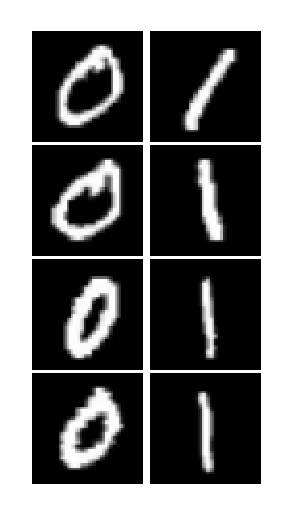
\includegraphics[width=0.045\textwidth]{PaperC/figures/mcts_tikz/vertical_rs/task1_only.eps}};
    \draw[<-] (v2) -- (v1);
    
    %%% Task 3 level
    \draw[draw=color3!50, fill=color3!10, very thick, rounded corners] (0,-4) rectangle (16,-6);
    \node[squarednode] (dataset3) at (1.,-5) { \textbf{Task 3} \\ 
\includegraphics[width=0.08\textwidth]{PaperC/figures/mcts_tikz/dataset_two_images/dataset3.eps}};
    \node[squarednode, text=color3] (v3_beg) at (5,-5) {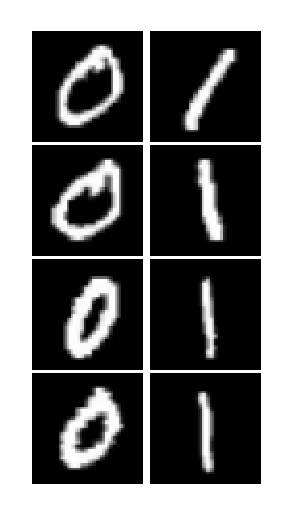
\includegraphics[width=0.045\textwidth]{PaperC/figures/mcts_tikz/vertical_rs/task1_only.eps}};
    \draw[<-, blue, very thick] (v3_beg) -- (v2);
    
    \node[squarednode, text=color3] (v3_mid) at (9,-5) {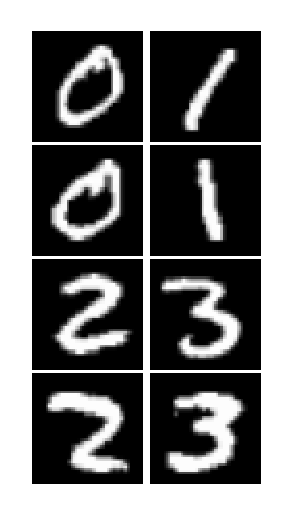
\includegraphics[width=0.045\textwidth]{PaperC/figures/mcts_tikz/vertical_rs/equal_task3.eps}};
    \draw[<-, red, very thick] (v3_mid) -- (v2);
    
    \node[squarednode, text=color3] (v3_end) at (13,-5) {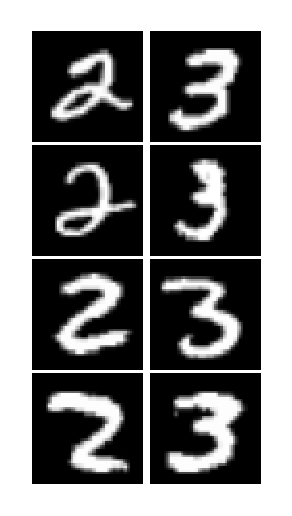
\includegraphics[width=0.045\textwidth]{PaperC/figures/mcts_tikz/vertical_rs/task2_only.eps}};
    \draw[<-, purple, very thick] (v3_end) -- (v2);
    
    %%% Task 4 level
    \draw[draw=magenta!50, fill=magenta!10, very thick, rounded corners] (0,-6) rectangle (16,-8);
    
    \node[squarednode] (dataset4) at (1.,-7) { \textbf{Task 4} \\ 
\includegraphics[width=0.08\textwidth]{PaperC/figures/mcts_tikz/dataset_two_images/dataset4.eps}};
    
    \node[squarednode, text=color3] (v41_beg) at (4,-7) {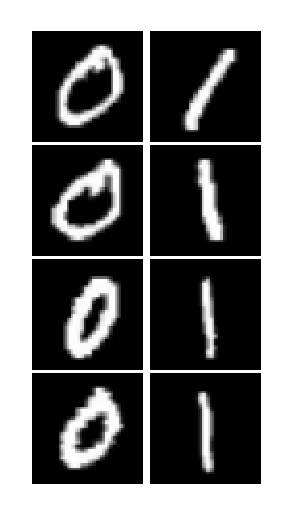
\includegraphics[width=0.045\textwidth]{PaperC/figures/mcts_tikz/vertical_rs/task1_only.eps}};
    \draw[<-, blue, very thick] (v41_beg) -- (v3_beg);
    %\draw[<-] (v4_beg) -- (v3_mid);
    %\draw[<-] (v4_beg) -- (v3_end);
    
    \node[] (v41_dots) at (5,-7) {\large $\cdots$};
    %\draw[<-] (v4_dots1) -- (v3_beg);%\draw[<-, dashed] (v4_dots1) -- (v3_beg);
    %\draw[<-] (v4_dots1) -- (v3_mid);
    %\draw[<-] (v4_dots1) -- (v3_end);
    
    \node[squarednode, text=color3] (v41_end) at (6,-7) {\includegraphics[width=0.045\textwidth]{PaperC/figures/mcts_tikz/vertical_rs/task3_only.eps}};
    \draw[<-] (v41_end) -- (v3_beg);
    
    \node[squarednode, text=color3] (v42_beg) at (7.1,-7) {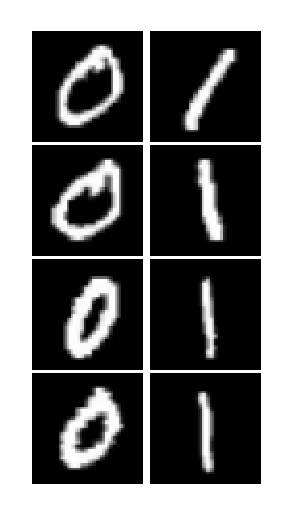
\includegraphics[width=0.045\textwidth]{PaperC/figures/mcts_tikz/vertical_rs/task1_only.eps}};
    \draw[<-] (v42_beg) -- (v3_mid);
    
    \node[] (v42_dots1) at (8,-7) {\large $\cdots$};
    
    \node[squarednode, text=color3] (v42_mid) at (9,-7) {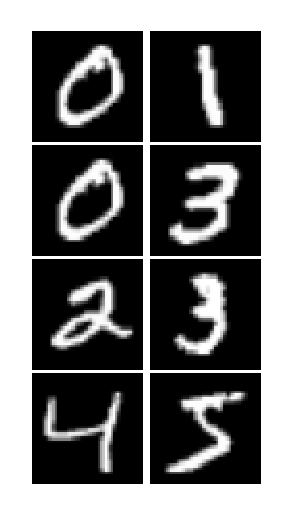
\includegraphics[width=0.045\textwidth]{PaperC/figures/mcts_tikz/vertical_rs/equal_task4.eps}};
    \draw[<-, red, very thick] (v42_mid) -- (v3_mid);
    
    \node[] (v42_dots2) at (10,-7) {\large $\cdots$};
    
    \node[squarednode, text=color3] (v42_end) at (11,-7) {\includegraphics[width=0.045\textwidth]{PaperC/figures/mcts_tikz/vertical_rs/task3_only.eps}};
    \draw[<-] (v42_end) -- (v3_mid);
    %\node[squarednode, text=color3] (v4_end1) at (6.5,-7) {\includegraphics[width=0.08\textwidth]{PaperC/figures/mcts_tikz/replay_batches/task3_only.eps}};
    %\draw[<-] (v4_end1) -- (v3_beg);
    
    \node[squarednode, text=color3] (v43_beg) at (12.1,-7) {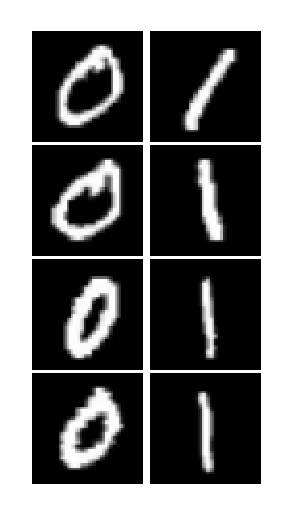
\includegraphics[width=0.045\textwidth]{PaperC/figures/mcts_tikz/vertical_rs/task1_only.eps}};
    \draw[<-] (v43_beg) -- (v3_end);
    
    \node[] (v43_dots) at (13,-7) {\large $\cdots$};
    %\draw[<-] (v4_dots2) -- (v3_beg);
    %\draw[<-] (v4_dots2) -- (v3_mid);
    %\draw[<-] (v4_dots2) -- (v3_end);
    
    \node[squarednode, text=color3] (v43_end) at (14,-7) {\includegraphics[width=0.045\textwidth]{PaperC/figures/mcts_tikz/vertical_rs/task3_only.eps}};
    \draw[<-, purple, very thick] (v43_end) -- (v3_end);
    %\draw[<-] (v4_end) -- (v3_mid);
    %\draw[<-, purple, very thick] (v4_end) -- (v3_end);


    %%% Task 5 level
    \draw[draw=green!50, fill=green!10, very thick, rounded corners] (0,-8) rectangle (16,-10);
    \node[squarednode] (dataset5) at (1.,-9) { \textbf{Task 5} \\ 
\includegraphics[width=0.08\textwidth]{PaperC/figures/mcts_tikz/dataset_two_images/dataset5.eps}};
    
    \node[squarednode, text=color3] (v51_beg) at (3,-9) {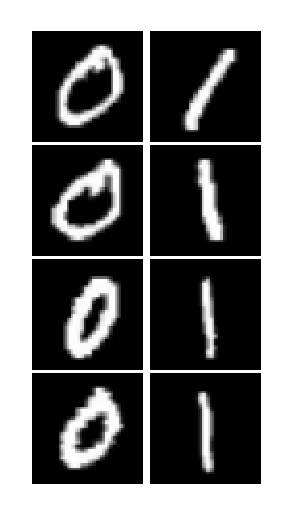
\includegraphics[width=0.045\textwidth]{PaperC/figures/mcts_tikz/vertical_rs/task1_only.eps}};
    \draw[<-, blue, very thick] (v51_beg) -- (v41_beg);
    %\draw[<-] (v5_beg) -- (v4_dots1);
    %\draw[<-] (v5_beg) -- (v4_mid);
    %\draw[<-] (v5_beg) -- (v4_dots2);
    %\draw[<-] (v5_beg) -- (v4_end);
    
    \node[] (v51_dots) at (4,-9) {\large $\cdots$};
    %\draw[<-] (v5_dots1) -- (v4_beg1);
    %\draw[<-] (v5_dots1) -- (v4_dots1);
    %\draw[<-] (v5_dots1) -- (v4_mid);
    %\draw[<-] (v5_dots1) -- (v4_dots2);
    %\draw[<-] (v5_dots1) -- (v4_end);
    
    \node[squarednode, text=color3] (v51_end) at (5,-9) {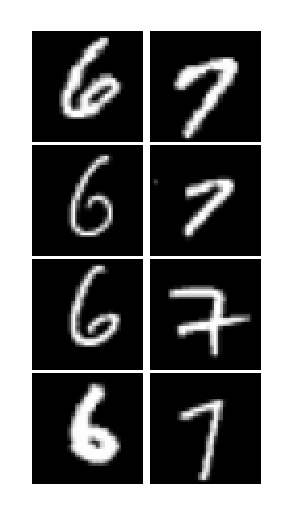
\includegraphics[width=0.045\textwidth]{PaperC/figures/mcts_tikz/vertical_rs/task4_only.eps}};
    \draw[<-] (v51_end) -- (v41_beg);
    
    %\node[squarednode, text=color3] (v52_beg) at (5,-9) {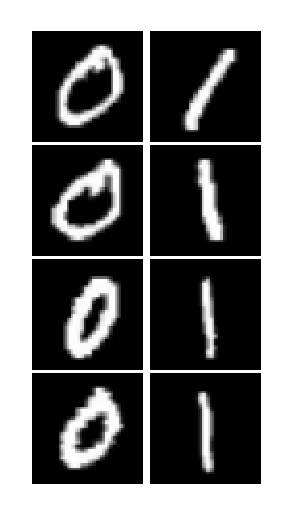
\includegraphics[width=0.045\textwidth]{PaperC/figures/mcts_tikz/vertical_rs/task1_only.eps}};
    
    %\node[squarednode, text=color3] (v5_mid_low) at (6,-9) {\includegraphics[width=0.06\textwidth]{PaperC/figures/mcts_tikz/replay_batches/task5_middle0.eps}};
    %\draw[<-] (v5_mid_low) -- (v4_beg);
    %\draw[<-] (v5_mid_low) -- (v4_dots1);
    %\draw[<-] (v5_mid_low) -- (v4_mid);
    %\draw[<-] (v5_mid_low) -- (v4_dots2);
    %\draw[<-] (v5_mid_low) -- (v4_end);
    
    \node[] (v52_dots) at (6,-9) {\large $\cdots$};
    \draw[<-, dashed] (v52_dots) -- (v41_end);
    
    \node[] (v53_dots) at (7.1,-9) {\large $\cdots$};
    \draw[<-, dashed] (v53_dots) -- (v42_beg);
    
     \node[] (v54_dots) at (8,-9) {\large $\cdots$};
    %\draw[<-] (v5_dots2) -- (v4_beg);
    %\draw[<-] (v5_dots2) -- (v4_dots1);
    %\draw[<-] (v5_dots2) -- (v4_mid);
    %\draw[<-] (v5_dots2) -- (v4_dots2);
    %\draw[<-] (v5_dots2) -- (v4_end);
    
    \node[squarednode, text=color3] (v52_mid) at (9,-9) {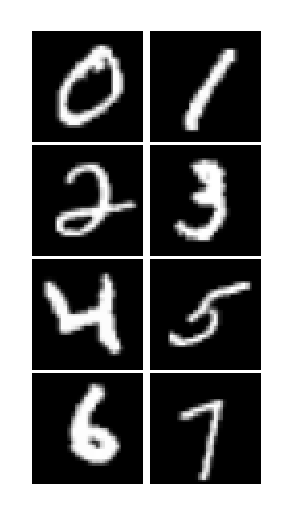
\includegraphics[width=0.045\textwidth]{PaperC/figures/mcts_tikz/vertical_rs/equal_task5.eps}};
    \draw[<-, red, very thick] (v52_mid) -- (v42_mid);
    %\draw[<-] (v5_mid) -- (v4_beg);
    %\draw[<-] (v5_mid) -- (v4_dots1);
    %\draw[<-, red, very thick] (v5_mid) -- (v4_mid);
    %\draw[<-] (v5_mid) -- (v4_dots2);
    %\draw[<-] (v5_mid) -- (v4_end);
    
    \node[] (v55_dots) at (10,-9) {\large $\cdots$};
    
    \node[] (v56_dots) at (11,-9) {\large $\cdots$};
    \draw[<-, dashed] (v56_dots) -- (v42_end);
    
    \node[] (v57_dots) at (12.1,-9) {\large $\cdots$};
    \draw[<-, dashed] (v57_dots) -- (v43_beg);
    %\draw[<-] (v5_dots3) -- (v4_beg);
    %\draw[<-] (v5_dots3) -- (v4_dots1);
    %\draw[<-] (v5_dots3) -- (v4_mid);
    %\draw[<-] (v5_dots3) -- (v4_dots2);
    %\draw[<-] (v5_dots3) -- (v4_end);
    
    %\node[squarednode, text=color3] (v5_mid_high) at (12,-9) {\includegraphics[width=0.06\textwidth]{PaperC/figures/mcts_tikz/replay_batches/task5_middle1.eps}};
    %\draw[<-] (v5_mid_high) -- (v4_beg);
    %\draw[<-] (v5_mid_high) -- (v4_dots1);
    %\draw[<-] (v5_mid_high) -- (v4_mid);
    %\draw[<-] (v5_mid_high) -- (v4_dots2);
    %\draw[<-] (v5_mid_high) -- (v4_end);
    
    \node[squarednode, text=color3] (v53_beg) at (13,-9) {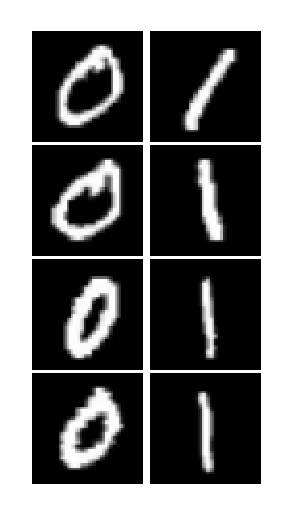
\includegraphics[width=0.045\textwidth]{PaperC/figures/mcts_tikz/vertical_rs/task1_only.eps}};
    \draw[<-] (v53_beg) -- (v43_end);
    
    \node[black] (v58_dots) at (14,-9) {\large $\cdots$};
    
    %\draw[--, dashed] (v5_dots4) -- (v43_dots);
    %\draw[<-] (v5_dots4) -- (v4_mid);
    %\draw[<-] (v5_dots4) -- (v4_dots2);
    %\draw[<-] (v5_dots4) -- (v4_end);
    
    \node[squarednode, text=color3] (v53_end) at (15,-9) {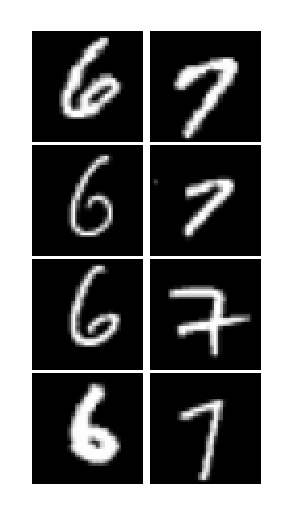
\includegraphics[width=0.045\textwidth]{PaperC/figures/mcts_tikz/vertical_rs/task4_only.eps}};
    \draw[<-, purple, very thick] (v53_end) -- (v43_end);
    %\draw[<-] (v5_end) -- (v4_beg);
    %\draw[<-] (v5_end) -- (v4_dots1);
    %\draw[<-] (v5_end) -- (v4_mid);
    %\draw[<-] (v5_end) -- (v4_dots2);
    %\draw[<-, purple, very thick] (v5_end) -- (v4_end);
\end{tikzpicture}
}
  % \tikzexternalenable
  % \vspace{-15pt}
  % \includegraphics[width=0.95\linewidth]{pixeldag.png}
  % \vspace{-15pt}

\vspace{-2mm}
\caption{An exemplar tree of replay memory compositions from the proposed discretization method described in Section \ref{sec:replay_scheduling_in_continual_learning} for Split MNIST. The replay memories from one replay schedule are found by traversing from task 1-5 through the tree on the right hand side. The replay memory compositions have been structured according to the task where they can be used for replay. Note that the replay memory at task 1 is the empty set, i.e., $\gM = \emptyset$. Example images for each task are shown on the left.
}
\vspace{-3mm}
\label{fig:replay_scheduling_mcts_tree_example}
\end{figure*}



\subsection{Replay Scheduling in Continual Learning}\label{sec:replay_scheduling_in_continual_learning}

In this section, 
we describe our replay scheduling method for selecting the replay memory at different time steps. We define a replay schedule as a sequence $S = (\va_1, \dots, \va_{T-1})$, where $\va_i = (a_1, \dots, a_{T-1})$ for $1 \leq i \leq T-1$ is the sequence of task proportions used for determining how many samples per task to fill the replay memory with at task $i$. To make the selection of task proportions tractable, we construct an action space with a discrete number of choices for %the 
task proportions from old tasks. 
We use the following method to construct this action space: At the time to learn task $t$, we have $t-1$ historical tasks that we can choose from. We create $t-1$ bins $\vb_t = [b_1, \dots, b_{t-1}]$ and choose a task index to sample for each bin $b_i \in \{1, \dots, t-1 \}$. We treat the bins as interchangeable and only keep the unique choices. 
For example, at task 3, we have seen task 1 and 2, so the unique choices of vectors are $[1,1], [1,2], [2,2]$, where $[1,1]$ indicates that all memory samples are from task 1, $[1,2]$ indicates that half memory is from task 1 and the other half are from task etc. The task proportions are then computed by counting the number of occurrences of each task index in $\vb_t$ and dividing by $t-1$, such that $\va_t = \texttt{bincount}(\vb_t) / (t-1)$. 
If the memory size $M$ is not divisible by the task proportion value for task $i$, we round the number of replay samples from task $i$, i.e., $a_i \cdot M$, up or down accordingly while keeping the memory size fixed.
From this specification, we can build a tree of different replay schedules to evaluate with the network.


Figure \ref{fig:replay_scheduling_mcts_tree_example} shows an example of a replay schedule tree with Split MNIST~\citep{zenke2017continual} 
where the memory size is $M=8$. %where the memory size has been set to $M=8$. 
The figure shows the current tasks with example images of the task classes on the left, and the right side shows examples of possible replay memories that can be evaluated. The memory starts as the empty set, i.e. $\gM_1 = \emptyset$, at task 1. Before learning task 2, $\gM_2$ is filled with $M$ task 1 examples since this is the only task seen so far. At task 3, the memory compositions we can choose from are $M$ examples from either task 1 or 2, as well as equally filling $\gM_3$ with four examples each from both tasks. 
A replay schedule is represented as a path traversal of different replay memory compositions from task 1 to task 5. We have color-coded three examples of possible schedules in Figure \ref{fig:replay_scheduling_mcts_tree_example} to use for illustration: the \textcolor{blue}{blue} path represents a replay schedule where only task 1 examples are replayed. %at all future tasks. 
The \textcolor{red}{red} path represents using an equally distributed amount of memory samples per task in the memory, and the \textcolor{purple}{purple} path represents a schedule where the memory is filled $M$ examples from the previously visited task. Note that all other possible paths in the tree are also valid replay schedules. 






\subsection{Monte Carlo Tree Search for Replay Schedules}
\label{paperC:sec:mcts_for_replay_scheduling}

In this section, we describe how we enable using MCTS for studying the benefits of replay scheduling in CL scenarios.
The tree-shaped action space of task proportions described in Section \ref{paperC:sec:replay_scheduling_in_continual_learning} grows fast with the number of tasks, which complicates studying replay scheduling in datasets with longer task-horizons. Since the search space is too big for using exhaustive searches, 
we need a scalable method that enables tree searches in large action spaces.
To this end, we propose to use MCTS since it has been successful in applications with large action spaces~\citeC{C:browne2012survey, C:chaudhry2018feature, C:gelly2006modification, C:silver2016mastering}. In our case, MCTS concentrates the search for replay schedules in directions with promising CL performance in the environment. We use MCTS in an ideal CL setting, wherein multiple episodes are allowed, for demonstration purposes to show that replay scheduling can be critical for the CL performance. 

Each memory composition in the action space corresponds to a node that can be visited by MCTS. For example, in Figure \ref{fig:replay_scheduling_mcts_tree_example}, the nodes correspond to the possible memory examples which can be visited during the MCTS rollouts.
At task $t$, the node $v_t$ is related to a task proportions $\va_{t}$ used for retrieving a replay memory from the historical data. 
We store the related task proportion $\va_t$ from every visited node $v_t$ in the replay schedule $S$. 
The final replay schedule is then used for constructing the replay memories at each task during the CL training.  
Next, we briefly outline the MCTS steps for performing the replay schedule search (more details in Appendix \ref{app:rs_mcts_algorithm}):

\vspace{-1mm}
\begin{itemize}[leftmargin=*, topsep=0pt, noitemsep, label={}]
	\item {\bf Selection.} During a rollout, the current node $v_t$ either moves randomly to unvisited children, or selects the next node by evaluating the Upper Confidence Tree (UCT)~\citeC{C:kocsis2006bandit} if all children has been visited earlier.
	The child $v_{t+1}$ with the highest UCT score is selected using the function from \cite{chaudhry2018feature}:
	\begin{align}\label{eq:uct}
		UCT(v_t, v_{t+1}) = \text{max}(q(v_{t+1})) + C \sqrt{\frac{2 \log(n(v_{t}))}{n(v_{t+1})}},
	\end{align}
	where $q(\cdot)$ is the reward function, $C$ the exploration constant, and $n(\cdot)$ the number of node visits. 
	
	\item {\bf Expansion.} Whenever the current node $v_t$ has unvisited child nodes, the search tree is expanded with one of the unvisited child nodes $v_{t+1}$ selected with uniform sampling. 
	
	\item {\bf Simulation and Reward.} After expansion, the succeeding nodes are selected randomly until reaching a terminal node $v_T$. The task proportions from the visited nodes in the rollout constitutes the replay schedule $S$. After training the network using $S$ for replay, we calculate the reward for the rollout is given by $r = \frac{1}{T} \sum_{i=1}^T A_{T, i}^{(val)}$, where $A_{T, i}^{(val)}$ is the validation accuracy of task $i$ at task $T$.  
	
	\item {\bf Backpropagation.} Reward $r$ is backpropagated from the expanded node $v_t$ to the root $v_1$, where the reward function $q(\cdot)$ and number of visits $n(\cdot)$ are updated at each node. 
\end{itemize}













\begin{figure}[t]
  \centering
  \setlength{\figwidth}{0.23\textwidth}
  \setlength{\figheight}{.13\textheight}
  


\pgfplotsset{every axis title/.append style={at={(0.5,0.79)}}}
\pgfplotsset{every tick label/.append style={font=\tiny}}
\pgfplotsset{every major tick/.append style={major tick length=2pt}}
\pgfplotsset{every minor tick/.append style={minor tick length=1pt}}
\pgfplotsset{every axis x label/.append style={at={(0.5,-0.34)}}}
\pgfplotsset{every axis y label/.append style={at={(-0.32,0.5)}}}
\begin{tikzpicture}
\tikzstyle{every node}=[font=\scriptsize]
\definecolor{color0}{rgb}{0.12156862745098,0.466666666666667,0.705882352941177}
\definecolor{color1}{rgb}{1,0.498039215686275,0.0549019607843137}
\definecolor{color2}{rgb}{0.172549019607843,0.627450980392157,0.172549019607843}
\definecolor{color3}{rgb}{0.83921568627451,0.152941176470588,0.156862745098039}
\definecolor{color4}{rgb}{0.580392156862745,0.403921568627451,0.741176470588235}

\begin{groupplot}[group style={group size= 6 by 1, horizontal sep=0.69cm, vertical sep=0.85cm}]

\input{PaperC/figures/mcts_rewards_comparison/MNIST_rewards}

\input{PaperC/figures/mcts_rewards_comparison/FashionMNIST_rewards}

\input{PaperC/figures/mcts_rewards_comparison/notMNIST_rewards}

\input{PaperC/figures/mcts_rewards_comparison/PermutedMNIST_rewards}

\input{PaperC/figures/mcts_rewards_comparison/CIFAR100_rewards}

\input{PaperC/figures/mcts_rewards_comparison/miniImagenet_rewards}

\end{groupplot}

\end{tikzpicture}
  \vspace{-3mm}
  \caption{ Average test accuracies over tasks after learning the final task (ACC) over the MCTS simulations for all datasets, where 'S' and 'P' are used as short for 'Split' and 'Permuted'. We compare performance for RS-MCTS (Ours) against random replay schedules (Random), Equal Task Schedule (ETS), and Heuristic Scheduling (Heuristic) baselines. 
  For the first three datasets, we show the best ACC found from a breadth-first search (BFS) as an upper bound. All results have been averaged over 5 seeds. These results show that replay scheduling can improve over ETS and outperform or perform on par with Heuristic across different datasets and network architectures. 
  }
  \label{fig:mcts_best_rewards}
  \vspace{-3mm}
\end{figure}




\section{Experiments}\label{paperC:sec:experiments}

We evaluated our replay scheduling method empirically on six common benchmark datasets for CL. 
%We show that scheduling of the replay memory improves significantly over replaying equal proportions across the tasks. 
%Furthermore, we demonstrate that replay scheduling can be as efficient as replaying all available memory samples in settings where only 1 example per class can be stored for replay. 
We denote our method as Replay Scheduling MCTS (RS-MCTS) and select the result on the held-out test sets from the replay schedule that yielded the best reward on the validation set during the search.
%We perform experiments using 5 different seeds on all datasets. 
%Our code is available as part of the supplementary material.
%Next, we briefly describe the experimental settings. 
Full details on experimental settings are in Appendix \ref{paperC:app:experimental_settings} and additional results are in Appendix \ref{paperC:app:additional_experimental_results}. %Additional information on experimental settings and results can be found in Appendix \ref{app:experimental_settings} and \ref{app:additional_experimental_results} respectively. 
Our code is available in the supplementary material. %as part of the supplementary material.

\vspace{-3mm}
\paragraph{Datasets.} We conduct experiments on six datasets commonly used as benchmarks in the CL literature: Split MNIST~\citeC{C:lecun1998gradient, C:zenke2017continual}, Fashion-MNIST~\citeC{C:xiao2017fashion}, Split notMNIST~\citeC{C:bulatov2011notMNIST}, Permuted MNIST~\citeC{C:goodfellow2013empirical}, Split CIFAR-100~\citeC{C:krizhevsky2009learning}, and Split miniImagenet~\citeC{C:vinyals2016matching}. We randomly sample 15\% of the training data from each task to use for validation when computing the reward for the MCTS simulations. 

\vspace{-3mm}
\paragraph{Baselines.} We compare RS-MCTS to using 1) random replay schedules (Random), 2) equal task schedules (ETS), and 3) a heuristic scheduling method (Heuristic). The ETS baseline uses equal task proportions, such that $M/(t-1)$ samples per task are replayed during learning of task $t$,and use both training and validations sets for training such that ETS use the same amount of data as RS-MCTS. %such that $M/(t-1)$ samples per task are replayed during learning of task $t$, and use both training and validations sets for training such that they use the same amount of data as RS-MCTS. 
The Heuristic baseline replays the tasks which accuracy on the validation set is below a certain threshold proportional to the best achieved validation accuracy on the task. Here, the replay memory is filled with $M/k$ samples per task where $k$ is the number of selected tasks. If $k=0$, then we skip applying replay at the current task.  
See Appendix \ref{paperC:app:heuristic_scheduling_baseline} for more details on the Heuristic baseline. 

%%% Table 1, put it here for placement

\begin{table}[t]
\footnotesize
\centering
\caption{
Performance comparison with ACC between RS-MCTS (Ours), Random scheduling (Random), Equal Task Schedule (ETS), and Heuristic Scheduling (Heuristic) with various memory selection methods evaluated across all datasets. 
%We use 'S' and 'P' as short for 'Split' and 'Permuted' for the datasets. 
Replay memory sizes are $M=10$ and $M=100$ for the 5-task and 10/20-task datasets respectively. We report the mean and standard deviation averaged over 5 seeds. Ours performs better or on par with the baselines on most datasets and selection methods, where MoF yields the best results %performance 
in general.
}
\vspace{-3mm}
%\setlength{\tabcolsep}{5pt}
\resizebox{\textwidth}{!}{ %\scalebox{0.87}{
\begin{tabular}{l l c c c c c c}
    \toprule
     & & \multicolumn{3}{c}{{\bf 5-task Datasets}} & \multicolumn{3}{c}{{\bf 10- and 20-task Datasets}} \\
    \cmidrule(lr){3-5} \cmidrule(lr){6-8}
    {\bf Selection} & {\bf Method} & S-MNIST & S-FashionMNIST & S-notMNIST & P-MNIST & S-CIFAR-100 & S-miniImagenet \\
    \midrule 
    \multirow{4}{*}{Uniform} & Random & 95.91 {\scriptsize ($\pm$ 1.56)}  & 95.82 {\scriptsize ($\pm$ 1.45)} & 92.39 {\scriptsize ($\pm$ 1.29)} & 72.44 {\scriptsize ($\pm$ 1.15)} & 53.99 {\scriptsize ($\pm$ 0.51)} & 48.08 {\scriptsize ($\pm$ 1.36)} \\
     & ETS  & 94.02 {\scriptsize ($\pm$ 4.25)} &  95.81 {\scriptsize ($\pm$ 3.53)} & 91.01 {\scriptsize ($\pm$ 1.39)} & 71.09 {\scriptsize ($\pm$ 2.31)} & 47.70 {\scriptsize ($\pm$ 2.16)} & 46.97 {\scriptsize ($\pm$ 1.24)} \\
     & Heuristic &  96.02 {\scriptsize ($\pm$ 2.32)} &  97.09 {\scriptsize ($\pm$ 0.62)} & 91.26 {\scriptsize ($\pm$ 3.99)} & {\bf 76.68} {\scriptsize ($\pm$ 2.13)} & {\bf 57.31} {\scriptsize ($\pm$ 1.21)} & 49.66 {\scriptsize ($\pm$ 1.10)} \\
     & Ours &  {\bf 97.93} {\scriptsize ($\pm$ 0.56)} &  {\bf 98.27} {\scriptsize ($\pm$ 0.17)} & {\bf 94.64} {\scriptsize ($\pm$ 0.39)} & 76.34 {\scriptsize ($\pm$ 0.98)} & 56.60 {\scriptsize ($\pm$ 1.13)} & {\bf 50.20} {\scriptsize ($\pm$ 0.72)} \\
    \midrule 
    \multirow{4}{*}{$k$-means} & Random & 94.24 {\scriptsize ($\pm$ 3.20)} & 96.30 {\scriptsize ($\pm$ 1.62)} & 91.64 {\scriptsize ($\pm$ 1.39)} & 74.30 {\scriptsize ($\pm$ 1.43)} & 53.18 {\scriptsize ($\pm$ 1.66)} & 49.47 {\scriptsize ($\pm$ 2.70)}  \\ 
     & ETS  & 92.89 {\scriptsize ($\pm$ 3.53)} & 96.47 {\scriptsize ($\pm$ 0.85)} & {\bf 93.80} {\scriptsize ($\pm$ 0.82)} & 69.40 {\scriptsize ($\pm$ 1.32)} & 47.51 {\scriptsize ($\pm$ 1.14)} & 45.82 {\scriptsize ($\pm$ 0.92)} \\
     & Heuristic &  96.28 {\scriptsize ($\pm$ 1.68)} &  95.78 {\scriptsize ($\pm$ 1.50)}  & 91.75 {\scriptsize ($\pm$ 0.94)} & 75.57 {\scriptsize ($\pm$ 1.18)} & 54.31 {\scriptsize ($\pm$  3.94)} & 49.25 {\scriptsize ($\pm$ 1.00)} \\
    & Ours & {\bf 98.20} {\scriptsize ($\pm$ 0.16)} & {\bf 98.48} {\scriptsize ($\pm$ 0.26)} &  93.61 {\scriptsize ($\pm$ 0.71)} & {\bf 77.74} {\scriptsize ($\pm$ 0.80)} & {\bf 56.95} {\scriptsize ($\pm$ 0.92)} & {\bf 50.47} {\scriptsize ($\pm$ 0.85)} \\  
    \midrule 
    \multirow{4}{*}{$k$-center} & Random & 96.40 {\scriptsize ($\pm$ 0.68)} & 95.57 {\scriptsize ($\pm$ 3.16)}  & 92.61 {\scriptsize ($\pm$ 1.70)} & 71.41 {\scriptsize ($\pm$ 2.75)} & 48.46 {\scriptsize ($\pm$ 0.31)} & 44.76 {\scriptsize ($\pm$ 0.96)} \\ 
     & ETS  & 94.84 {\scriptsize ($\pm$ 1.40)} & 97.28 {\scriptsize ($\pm$ 0.50)} & 91.08 {\scriptsize ($\pm$ 2.48)} & 69.11 {\scriptsize ($\pm$ 1.69)} & 44.13 {\scriptsize ($\pm$ 1.06)} & 41.35 {\scriptsize ($\pm$ 1.23)} \\
     & Heuristic & 94.55 {\scriptsize ($\pm$ 2.79)} & 94.08 {\scriptsize ($\pm$ 3.72)} & 92.06 {\scriptsize ($\pm$ 1.20)} & 74.33 {\scriptsize ($\pm$ 2.00)} & 50.32 {\scriptsize ($\pm$ 1.97)} & 44.13 {\scriptsize ($\pm$ 0.95)} \\
     & Ours & {\bf 98.24} {\scriptsize ($\pm$ 0.36)} & {\bf 98.06} {\scriptsize ($\pm$ 0.35)} & {\bf 94.26} {\scriptsize ($\pm$ 0.37)} & {\bf 76.55} {\scriptsize ($\pm$ 1.16)} & {\bf 51.37} {\scriptsize ($\pm$ 1.63)} & {\bf 46.76} {\scriptsize ($\pm$ 0.96)}  \\  
    \midrule 
    \multirow{4}{*}{MoF} & Random & 95.18 {\scriptsize ($\pm$ 3.18)} & 95.76 {\scriptsize ($\pm$ 1.41)}  & 91.33 {\scriptsize ($\pm$ 1.75)} & 77.96 {\scriptsize ($\pm$ 1.84)} & 61.93 {\scriptsize ($\pm$ 1.05)} & 54.50 {\scriptsize ($\pm$ 1.33)} \\ 
     & ETS & 97.04 {\scriptsize ($\pm$ 1.23)} & 96.48 {\scriptsize ($\pm$ 1.33)} & 92.64 {\scriptsize ($\pm$ 0.87)} & 77.62 {\scriptsize ($\pm$ 1.12)} & 60.43 {\scriptsize ($\pm$ 1.17)} & 56.12 {\scriptsize ($\pm$ 1.12)} \\
     & Heuristic & 96.46 {\scriptsize ($\pm$ 2.41)} &  95.84 {\scriptsize ($\pm$ 0.89)} & 93.24 {\scriptsize ($\pm$ 0.77)} & 77.27 {\scriptsize ($\pm$ 1.45)} & 55.60 {\scriptsize ($\pm$ 2.70)} & 52.30 {\scriptsize ($\pm$ 0.59)} \\
     & Ours & {\bf 98.37} {\scriptsize ($\pm$ 0.24)} & {\bf 97.84} {\scriptsize ($\pm$ 0.32)} & {\bf 94.62} {\scriptsize ($\pm$ 0.42)} & {\bf 81.58} {\scriptsize ($\pm$ 0.75)} & {\bf 64.22} {\scriptsize ($\pm$ 0.65)} & {\bf 57.70} {\scriptsize ($\pm$ 0.51)} \\
    \bottomrule
\end{tabular}
}
\vspace{-3mm}
\label{tab:results_memory_selection_methods}
\end{table}

\begin{comment}
\begin{table*}[t]
\footnotesize
\centering
\caption{
Performance comparison between RS-MCTS (Ours), Random scheduling (Random), Equal Task Schedule (ETS), and Heuristic Scheduling (Heuristic) with various memory selection methods evaluated across all datasets. 
%We use 'S' and 'P' as short for 'Split' and 'Permuted' for the datasets. 
The replay memory size is $M=10$ and $M=100$ for the 5-task and 10/20-task datasets respectively. We report the mean and standard deviation averaged over 5 seeds. RS-MCTS performs better or on par than the baselines on most datasets and selection methods, where MoF yields the best results %performance 
in general.
}
%\vspace{-3mm}
%\setlength{\tabcolsep}{5pt}
\scalebox{0.87}{
\begin{tabular}{l l c c c c c c}
    \toprule
     & & \multicolumn{3}{c}{{\bf 5-task Datasets}} & \multicolumn{3}{c}{{\bf 10- and 20-task Datasets}} \\
    \cmidrule(lr){3-5} \cmidrule(lr){6-8}
    {\bf Selection} & {\bf Method} & S-MNIST & S-FashionMNIST & S-notMNIST & P-MNIST & S-CIFAR-100 & S-miniImagenet \\
    \midrule 
    \multirow{4}{*}{Uniform} & Random & 95.91 {\scriptsize ($\pm$ 1.56)}  & 95.82 {\scriptsize ($\pm$ 1.45)} & 92.39 {\scriptsize ($\pm$ 1.29)} & 72.44 {\scriptsize ($\pm$ 1.15)} & 53.99 {\scriptsize ($\pm$ 0.51)} & 48.08 {\scriptsize ($\pm$ 1.36)} \\
     & ETS  & 94.02 {\scriptsize ($\pm$ 4.25)} &  95.81 {\scriptsize ($\pm$ 3.53)} & 91.01 {\scriptsize ($\pm$ 1.39)} & 71.09 {\scriptsize ($\pm$ 2.31)} & 47.70 {\scriptsize ($\pm$ 2.16)} & 46.97 {\scriptsize ($\pm$ 1.24)} \\
     & Heuristic &  96.02 {\scriptsize ($\pm$ 2.32)} &  97.09 {\scriptsize ($\pm$ 0.62)} & 91.26 {\scriptsize ($\pm$ 3.99)} & 76.68 {\scriptsize ($\pm$ 2.13)} & 57.31 {\scriptsize ($\pm$ 1.21)} & 49.66 {\scriptsize ($\pm$ 1.10)} \\
     & Ours &  97.93 {\scriptsize ($\pm$ 0.56)} &  98.27 {\scriptsize ($\pm$ 0.17)} & 94.64 {\scriptsize ($\pm$ 0.39)} & 76.34 {\scriptsize ($\pm$ 0.98)} & 56.60 {\scriptsize ($\pm$ 1.13)} & 50.20 {\scriptsize ($\pm$ 0.72)} \\
    \midrule 
    \multirow{4}{*}{$k$-means} & Random & 94.24 {\scriptsize ($\pm$ 3.20)} & 96.30 {\scriptsize ($\pm$ 1.62)} & 91.64 {\scriptsize ($\pm$ 1.39)} & 74.30 {\scriptsize ($\pm$ 1.43)} & 53.18 {\scriptsize ($\pm$ 1.66)} & 49.47 {\scriptsize ($\pm$ 2.70)}  \\ 
     & ETS  & 92.89 {\scriptsize ($\pm$ 3.53)} & 96.47 {\scriptsize ($\pm$ 0.85)} & 93.80 {\scriptsize ($\pm$ 0.82)} & 69.40 {\scriptsize ($\pm$ 1.32)} & 47.51 {\scriptsize ($\pm$ 1.14)} & 45.82 {\scriptsize ($\pm$ 0.92)} \\
     & Heuristic &  96.28 {\scriptsize ($\pm$ 1.68)} &  95.78 {\scriptsize ($\pm$ 1.50)}  & 91.75 {\scriptsize ($\pm$ 0.94)} & 75.57 {\scriptsize ($\pm$ 1.18)} & 54.31 {\scriptsize ($\pm$  3.94)} & 49.25 {\scriptsize ($\pm$ 1.00)} \\
    & Ours & 98.20 {\scriptsize ($\pm$ 0.16)} & 98.48 {\scriptsize ($\pm$ 0.26)} &  93.61 {\scriptsize ($\pm$ 0.71)} & 77.74 {\scriptsize ($\pm$ 0.80)} & 56.95 {\scriptsize ($\pm$ 0.92)} & 50.47 {\scriptsize ($\pm$ 0.85)} \\  
    \midrule 
    \multirow{4}{*}{$k$-center} & Random & 96.40 {\scriptsize ($\pm$ 0.68)} & 95.57 {\scriptsize ($\pm$ 3.16)}  & 92.61 {\scriptsize ($\pm$ 1.70)} & 71.41 {\scriptsize ($\pm$ 2.75)} & 48.46 {\scriptsize ($\pm$ 0.31)} & 44.76 {\scriptsize ($\pm$ 0.96)} \\ 
     & ETS  & 94.84 {\scriptsize ($\pm$ 1.40)} & 97.28 {\scriptsize ($\pm$ 0.50)} & 91.08 {\scriptsize ($\pm$ 2.48)} & 69.11 {\scriptsize ($\pm$ 1.69)} & 44.13 {\scriptsize ($\pm$ 1.06)} & 41.35 {\scriptsize ($\pm$ 1.23)} \\
     & Heuristic & 94.55 {\scriptsize ($\pm$ 2.79)} & 94.08 {\scriptsize ($\pm$ 3.72)} & 92.06 {\scriptsize ($\pm$ 1.20)} & 74.33 {\scriptsize ($\pm$ 2.00)} & 50.32 {\scriptsize ($\pm$ 1.97)} & 44.13 {\scriptsize ($\pm$ 0.95)} \\
     & Ours & 98.24 {\scriptsize ($\pm$ 0.36)} & 98.06 {\scriptsize ($\pm$ 0.35)} & 94.26 {\scriptsize ($\pm$ 0.37)} & 76.55 {\scriptsize ($\pm$ 1.16)} & 51.37 {\scriptsize ($\pm$ 1.63)} & 46.76 {\scriptsize ($\pm$ 0.96)}  \\  
    \midrule 
    \multirow{4}{*}{MoF} & Random & 95.18 {\scriptsize ($\pm$ 3.18)} & 95.76 {\scriptsize ($\pm$ 1.41)}  & 91.33 {\scriptsize ($\pm$ 1.75)} & 77.96 {\scriptsize ($\pm$ 1.84)} & 61.93 {\scriptsize ($\pm$ 1.05)} & 54.50 {\scriptsize ($\pm$ 1.33)} \\ 
     & ETS & 97.04 {\scriptsize ($\pm$ 1.23)} & 96.48 {\scriptsize ($\pm$ 1.33)} & 92.64 {\scriptsize ($\pm$ 0.87)} & 77.62 {\scriptsize ($\pm$ 1.12)} & 60.43 {\scriptsize ($\pm$ 1.17)} & 56.12 {\scriptsize ($\pm$ 1.12)} \\
     & Heuristic & 96.46 {\scriptsize ($\pm$ 2.41)} &  95.84 {\scriptsize ($\pm$ 0.89)} & 93.24 {\scriptsize ($\pm$ 0.77)} & 77.27 {\scriptsize ($\pm$ 1.45)} & 55.60 {\scriptsize ($\pm$ 2.70)} & 52.30 {\scriptsize ($\pm$ 0.59)} \\
     & Ours & 98.37 {\scriptsize ($\pm$ 0.24)} & 97.84 {\scriptsize ($\pm$ 0.32)} & 94.62 {\scriptsize ($\pm$ 0.42)} & 81.58 {\scriptsize ($\pm$ 0.75)} & 64.22 {\scriptsize ($\pm$ 0.65)} & 57.70 {\scriptsize ($\pm$ 0.51)} \\
    \bottomrule
\end{tabular}
}
\vspace{-3mm}
\label{tab:results_memory_selection_methods}
\end{table*}
\end{comment}


\begin{comment}
\begin{table*}[t]
\footnotesize
\centering
\caption{
Accuracy comparison between RS-MCTS (Ours), Random choice scheduling (Random), Heuristic Scheduling (Heuristic), and Equal Task Schedule (ETS) with various memory selection methods evaluated across all datasets. We use 'S' and 'P' as short for 'Split' and 'Permuted' for the datasets. The replay memory size is $M=10$ and $M=100$ for the 5-task and 10/20-task datasets respectively. We report the mean and standard deviation averaged over 5 seeds. RS-MCTS performs better or on par than the baselines on most datasets and selection methods, where MoF yields the best performance in general.
}
%\vspace{-3mm}
\setlength{\tabcolsep}{5pt}
\begin{tabular}{l l c c c c c c}
    \toprule
     & & \multicolumn{3}{c}{{\bf 5-task Datasets}} & \multicolumn{3}{c}{{\bf 10- and 20-task Datasets}} \\
    \cmidrule(lr){3-5} \cmidrule(lr){6-8}
    {\bf Selection} & {\bf Method} & S-MNIST & S-FashionMNIST & S-notMNIST & P-MNIST & S-CIFAR-100 & S-miniImagenet \\
    \midrule 
    \multirow{4}{*}{Uniform} & Random & 95.91 $\pm$ 1.56  & 95.82 $\pm$ 1.45 & 92.39 $\pm$ 1.29 & 72.44 $\pm$ 1.15 & 53.99 $\pm$ 0.51 & 48.08 $\pm$ 1.36 \\
     & ETS  & 94.02 $\pm$ 4.25 &  95.81 $\pm$ 3.53 & 91.01 $\pm$ 1.39 & 71.09 $\pm$ 2.31 & 47.70 $\pm$ 2.16 & 46.97 $\pm$ 1.24 \\
     & Heuristic &  96.02 $\pm$ 2.32 &  97.09 $\pm$ 0.62 & 91.26 $\pm$ 3.99 & 76.68 $\pm$ 2.13 & 57.31 $\pm$ 1.21 & 49.66 $\pm$ 1.10 \\
     & Ours &  97.93 $\pm$ 0.56 &  98.27 $\pm$ 0.17 & 94.64 $\pm$ 0.39 & 76.34 $\pm$ 0.98 & 56.60 $\pm$ 1.13 & 50.20 $\pm$ 0.72 \\
    \midrule 
    \multirow{4}{*}{$k$-means} & Random & 94.24 $\pm$ 3.20 & 96.30 $\pm$ 1.62 & 91.64 $\pm$ 1.39 & 74.30 $\pm$ 1.43 & 53.18 $\pm$ 1.66 & 49.47 $\pm$ 2.70  \\ 
     & ETS  & 92.89 $\pm$ 3.53 & 96.47 $\pm$ 0.85 & 93.80 $\pm$ 0.82 & 69.40 $\pm$ 1.32 & 47.51 $\pm$ 1.14 & 45.82 $\pm$ 0.92 \\
     & Heuristic &  96.28 $\pm$ 1.68 &  95.78 $\pm$ 1.50  & 91.75 $\pm$ 0.94 & 75.57 $\pm$ 1.18 & 54.31 $\pm$  3.94 & 49.25 $\pm$ 1.00 \\
    & Ours & 98.20 $\pm$ 0.16 & 98.48 $\pm$ 0.26 &  93.61 $\pm$ 0.71 & 77.74 $\pm$ 0.80 & 56.95 $\pm$ 0.92 & 50.47 $\pm$ 0.85 \\  
    \midrule 
    \multirow{4}{*}{$k$-center} & Random & 96.40 $\pm$ 0.68 & 95.57 $\pm$ 3.16  & 92.61 $\pm$ 1.70 & 71.41 $\pm$ 2.75 & 48.46 $\pm$ 0.31 & 44.76 $\pm$ 0.96 \\ 
     & ETS  & 94.84 $\pm$ 1.40 & 97.28 $\pm$ 0.50 & 91.08 $\pm$ 2.48 & 69.11 $\pm$ 1.69 & 44.13 $\pm$ 1.06 & 41.35 $\pm$ 1.23 \\
     & Heuristic & 94.55 $\pm$ 2.79 & 94.08 $\pm$ 3.72 & 92.06 $\pm$ 1.20 & 74.33 $\pm$ 2.00 & 50.32 $\pm$ 1.97 & 44.13 $\pm$ 0.95 \\
     & Ours & {98.24 $\pm$ 0.36} & 98.06 $\pm$ 0.35 & 94.26 $\pm$ 0.37 & 76.55 $\pm$ 1.16 & {51.37 $\pm$ 1.63} & { 46.76 $\pm$ 0.96}  \\  
    \midrule 
    \multirow{4}{*}{MoF} & Random & 95.18 $\pm$ 3.18 & 95.76 $\pm$ 1.41  & 91.33 $\pm$ 1.75 & 77.96 $\pm$ 1.84 & 61.93 $\pm$ 1.05 & 54.50 $\pm$ 1.33 \\ 
     & ETS & 97.04 $\pm$ 1.23 & 96.48 $\pm$ 1.33 & 92.64 $\pm$ 0.87 & 77.62 $\pm$ 1.12 & 60.43 $\pm$ 1.17 & 56.12 $\pm$ 1.12 \\
     & Heuristic & 96.46 $\pm$ 2.41 &  95.84 $\pm$ 0.89 & 93.24 $\pm$ 0.77 & 77.27 $\pm$ 1.45 & 55.60 $\pm$ 2.70 & 52.30 $\pm$ 0.59 \\
     & Ours & { 98.37 $\pm$ 0.24} & { 97.84 $\pm$ 0.32} & {94.62 $\pm$ 0.42} & {81.58 $\pm$ 0.75} & {64.22 $\pm$ 0.65} & { 57.70 $\pm$ 0.51} \\
    \bottomrule
\end{tabular}
\vspace{-3mm}
\label{tab:results_memory_selection_methods}
\end{table*}
\end{comment}




\vspace{-3mm}
\paragraph{Architectures.} We use a multi-head output layer for all datasets except for Permuted MNIST where the network uses single-head output. We use a 2-layer MLP with 256 hidden units for Split MNIST, Split FashionMNIST, Split notMNIST, and Permuted MNIST. For Split CIFAR-100, we use the CNN architecture used in Vinyals \etal~\citeC{C:vinyals2016matching} and Schwartz \etal~\citeC{C:schwarz2018progress}. For Split miniImagenet, we apply the reduced ResNet-18 from \citeC{C:lopez2017gradient}. 

\vspace{-3mm}
\paragraph{Evaluation Metric.} We use the average test accuracy over all tasks after learning the final task, i.e., $\text{ACC} = \frac{1}{T} \sum_{i=1}^{T} A_{T, i}$ where $A_{T, i}$ is the test accuracy of task $i$ after learning task $T$. We report means and standard deviations of ACC using 5 different seeds on all datasets. 



%%% MCTS Results

%

\begin{figure}[t]
  \centering
  \setlength{\figwidth}{0.23\textwidth}
  \setlength{\figheight}{.13\textheight}
  \input{PaperC/figures/mcts_rewards_comparison/mcts_rewards_groupplot_single_row}
  \vspace{-3mm}
  \caption{ Average test accuracies over tasks after learning the final task (ACC) over the MCTS simulations for all datasets, where 'S' and 'P' are used as short for 'Split' and 'Permuted'. We compare performance for RS-MCTS (Ours) against random replay schedules (Random), Equal Task Schedule (ETS), and Heuristic Scheduling (Heuristic) baselines. 
  For the first three datasets, we show the best ACC found from a breadth-first search (BFS) as an upper bound. All results have been averaged over 5 seeds. These results show that replay scheduling can improve over ETS and outperform or perform on par with Heuristic across different datasets and network architectures. 
  }
  \label{fig:mcts_best_rewards}
  \vspace{-3mm}
\end{figure}




\subsection{Performance Progress of RS-MCTS}\label{paperC:sec:results_with_mcts}

In the first experiments, we show that the replay schedules from RS-MCTS yield better performance than replaying an equal amount of samples per task. 
The replay memory size is fixed to $M=10$ for Split MNIST, FashionMNIST, and notMNIST, and $M=100$ for Permuted MNIST, Split CIFAR-100, and Split miniImagenet. Uniform sampling is used as the memory selection method for all methods in this experiment.
For the 5-task datasets, we provide the optimal replay schedule found from a breadth-first search (BFS) over all 1050 possible replay schedules in our action space (which corresponds to a tree with depth of 4) as an upper bound for RS-MCTS. As the search space grows fast with the number of tasks, BFS becomes computationally infeasible when we have 10 or more tasks.


Figure \ref{fig:mcts_best_rewards} shows the progress of ACC over %the MCTS
iterations by RS-MCTS for all datasets. We also show the best ACC metrics for Random, ETS, Heuristic, and BFS (where appropriate) as straight lines. 
Furthermore, we include the ACC achieved by training on all seen datasets jointly at every task (Joint) for the 5-task datasets.
We observe that RS-MCTS outperforms Random and ETS successively with more iterations. Furthermore, RS-MCTS approaches the upper limit of BFS on the 5-task datasets. For Permuted MNIST and Split CIFAR-100, the Heuristic baseline and RS-MCTS perform on par after 50 iterations. This shows that Heuristic with careful tuning of the validation accuracy threshold can be a strong baseline when comparing replay scheduling methods. Table \ref{tab:results_memory_selection_methods} at the rows for Uniform selection shows the ACC for each method in this experiment. We note that RS-MCTS outperforms ETS significantly on most datasets and performs on par with Heuristic. 





%%% Table 2, put it here for placement

\begin{table}[t]
\footnotesize
\centering
\caption{
    Performance comparison with ACC between scheduling methods RS-MCTS (Ours), Random, ETS, and Heuristic combined with replay-based methods HAL, MER, DER, and DER++. %such as Hindsight Anchor Learning (HAL), Meta Experience Replay (MER), Dark Experience Replay (DER), and DER++. 
    Replay memory sizes are $M=10$ and $M=100$ for the 5-task and 10/20-task datasets respectively. We report the mean and standard deviation averaged over 5 seeds. Results on Heuristic where some seed did not converge is denoted by $^{*}$. Applying RS-MCTS to each method can enhance the performance compared to using the baseline schedules. 
}
%\vspace{-3mm}
%\setlength{\tabcolsep}{5pt}
\scalebox{0.87}{
\begin{tabular}{l l c c c c c c}
    \toprule
     & & \multicolumn{3}{c}{{\bf 5-task Datasets}} & \multicolumn{3}{c}{{\bf 10- and 20-task Datasets}} \\
    \cmidrule(lr){3-5} \cmidrule(lr){6-8}
    {\bf Method} & {\bf Schedule}  & S-MNIST & S-FashionMNIST & S-notMNIST & P-MNIST & S-CIFAR-100 & S-miniImagenet \\
    \midrule
    \multirow{4}{*}{HAL} & Random & 97.24 {\scriptsize ($\pm$ 0.70)}  & 86.74 {\scriptsize ($\pm$ 6.05)} & 93.61 {\scriptsize($\pm$ 1.31)}  & 88.49 {\scriptsize ($\pm$ 0.99)}  & 36.09 {\scriptsize ($\pm$ 1.77)} & 38.51 {\scriptsize ($\pm$ 2.22)} \\
     & ETS  & 94.02 {\scriptsize ($\pm$ 4.25)} &  95.81 {\scriptsize ($\pm$ 3.53)} & 91.01 {\scriptsize ($\pm$ 1.39)} & 88.46 {\scriptsize ($\pm$ 0.86)}  & 34.90 {\scriptsize ($\pm$ 2.02)} & 38.13 {\scriptsize ($\pm$ 1.18)} \\
    & Heuristic & 97.69 {\scriptsize ($\pm$ 0.19)} & $^{*}$74.16 {\scriptsize ($\pm$ 11.19)} & 93.64 {\scriptsize ($\pm$ 0.93)} & $^{*}$66.63 {\scriptsize ($\pm$ 28.50)} & 35.07 {\scriptsize($\pm$ 1.29)} & 39.51 {\scriptsize($\pm$ 1.49)} \\
     & Ours &  {\bf 97.93} {\scriptsize ($\pm$ 0.56)} &  {\bf 98.27} {\scriptsize ($\pm$ 0.17)} & {\bf 94.64} {\scriptsize ($\pm$ 0.39)} & {\bf 89.14} {\scriptsize ($\pm$ 0.74)}  & {\bf 40.22} {\scriptsize ($\pm$ 1.57)} & {\bf 41.39} {\scriptsize ($\pm$ 1.15)} \\
    \midrule 
    \multirow{4}{*}{MER} & Random & 93.07 {\scriptsize ($\pm$ 0.81)} & 85.53 {\scriptsize ($\pm$ 3.30)} & 91.13 {\scriptsize ($\pm$ 0.86)} & 75.90 {\scriptsize ($\pm$ 1.34)} & 42.96 {\scriptsize ($\pm$ 1.70)} & 31.48 {\scriptsize ($\pm$ 1.65)}  \\ 
     & ETS  & 92.89 {\scriptsize ($\pm$ 3.53)} & 96.47 {\scriptsize ($\pm$ 0.85)} & {\bf 93.80} {\scriptsize ($\pm$ 0.82)} & 73.01 {\scriptsize ($\pm$ 0.96)} & 43.38 {\scriptsize ($\pm$ 1.81)} & 33.58 {\scriptsize ($\pm$ 1.53)} \\
    & Heuristic & 94.30 {\scriptsize ($\pm$ 2.79)} & 96.91 {\scriptsize ($\pm$ 0.62)} & 90.90 {\scriptsize ($\pm$ 1.30)} & {\bf 83.86} {\scriptsize ($\pm$ 3.19)} & 40.90 {\scriptsize ($\pm$ 1.70)}  & {\bf 34.22} {\scriptsize ($\pm$ 1.93)} \\
    & Ours &  {\bf 98.20} {\scriptsize ($\pm$ 0.16)} & {\bf 98.48} {\scriptsize ($\pm$ 0.26)} &  93.61 {\scriptsize ($\pm$ 0.71)} & 79.72 {\scriptsize ($\pm$ 0.71)} & {\bf 44.29} {\scriptsize ($\pm$ 0.69)} & 32.74 {\scriptsize ($\pm$ 1.29)} \\  
    \midrule 
    \multirow{4}{*}{DER} & Random & 98.23 {\scriptsize ($\pm$ 0.53)} & 96.56 {\scriptsize ($\pm$ 1.79)}  & 92.89 {\scriptsize ($\pm$ 0.86)} & 87.51 {\scriptsize ($\pm$ 1.10)} & 56.83 {\scriptsize ($\pm$ 0.76)} & 42.19  {\scriptsize ($\pm$ 0.67)} \\ 
     & ETS  & 98.17 {\scriptsize ($\pm$ 0.35)} & 97.69 {\scriptsize ($\pm$ 0.58)} & 94.74 {\scriptsize ($\pm$ 1.05)} & 85.71 {\scriptsize ($\pm$ 0.75)} & 52.58 {\scriptsize ($\pm$ 1.49)} & 35.50  {\scriptsize ($\pm$ 2.84)} \\
    & Heuristic & 94.57 {\scriptsize ($\pm$ 1.71)} & $^{*}$72.49 {\scriptsize ($\pm$ 19.32)} & $^{*}$77.88 {\scriptsize ($\pm$ 12.58)} & 81.56 {\scriptsize ($\pm$ 2.28)} & 55.75 {\scriptsize ($\pm$ 1.08)} & {\bf 43.62} {\scriptsize ($\pm$ 0.88)} \\
     & Ours & {\bf 99.02} {\scriptsize ($\pm$ 0.10)} & {\bf 98.33} {\scriptsize ($\pm$ 0.51)} & {\bf 95.02} {\scriptsize ($\pm$ 0.33)} & {\bf 90.11} {\scriptsize ($\pm$ 0.18)} & {\bf 58.99} {\scriptsize ($\pm$ 0.98)} & 43.46  {\scriptsize ($\pm$ 0.95)}  \\  
    \midrule 
    \multirow{4}{*}{DER++} & Random & 97.90 {\scriptsize ($\pm$ 0.52)} & 97.10 {\scriptsize ($\pm$ 1.03)}  & 93.29 {\scriptsize ($\pm$ 1.43)} & 87.89 {\scriptsize ($\pm$ 1.10)} & 58.49  {\scriptsize ($\pm$ 1.44)} & 48.40  {\scriptsize ($\pm$ 0.69)} \\ 
     & ETS & 97.98 {\scriptsize ($\pm$ 0.52)} & 98.12 {\scriptsize ($\pm$ 0.40)} & 94.53 {\scriptsize ($\pm$ 1.02)} & 85.25 {\scriptsize ($\pm$ 0.88)} & 52.54  {\scriptsize ($\pm$ 1.06)} & 41.36  {\scriptsize ($\pm$ 2.90)} \\
    & Heuristic & 92.35 {\scriptsize ($\pm$ 2.42)} & $^{*}$67.31 {\scriptsize ($\pm$ 21.20)} & 93.88 {\scriptsize ($\pm$ 1.33)} & 79.17 {\scriptsize ($\pm$ 2.44)} & 56.70 {\scriptsize ($\pm$ 1.27)} & 45.73 {\scriptsize ($\pm$ 0.84)} \\
     & Ours & {\bf 98.84} {\scriptsize ($\pm$ 0.21)} & {\bf 98.38} {\scriptsize ($\pm$ 0.43)} & {\bf 94.73} {\scriptsize ($\pm$ 0.20)} & {\bf 89.84} {\scriptsize ($\pm$ 0.22)} & {\bf 59.23}  {\scriptsize ($\pm$ 0.83)} & {\bf 49.45}  {\scriptsize ($\pm$ 0.68)} \\
    \bottomrule
\end{tabular}
}
\vspace{-3mm}
\label{tab:results_applying_scheduling_to_recent_replay_methods}
\end{table}

\begin{comment}

\begin{table*}[t]
\footnotesize
\centering
\caption{
    Performance comparison between scheduling methods RS-MCTS (Ours), Random, ETS, and Heuristic when combining them with replay-based methods HAL, MER, DER, and DER++. %such as Hindsight Anchor Learning (HAL), Meta Experience Replay (MER), Dark Experience Replay (DER), and DER++. 
    Replay memory sizes are $M=10$ and $M=100$ for the 5-task and 10/20-task datasets respectively. We report the mean and standard deviation averaged over 5 seeds. Results on Heuristic where some seed did not converge is denoted by $^{*}$. Applying RS-MCTS to each method can enhance the performance compared to using the baseline schedules. 
}
%\vspace{-3mm}
%\setlength{\tabcolsep}{5pt}
\scalebox{0.87}{
\begin{tabular}{l l c c c c c c}
    \toprule
     & & \multicolumn{3}{c}{{\bf 5-task Datasets}} & \multicolumn{3}{c}{{\bf 10- and 20-task Datasets}} \\
    \cmidrule(lr){3-5} \cmidrule(lr){6-8}
    {\bf Method} & {\bf Schedule}  & S-MNIST & S-FashionMNIST & S-notMNIST & P-MNIST & S-CIFAR-100 & S-miniImagenet \\
    \midrule
    \multirow{4}{*}{HAL} & Random & 97.24 {\scriptsize ($\pm$ 0.70)}  & 86.74 {\scriptsize ($\pm$ 6.05)} & 93.61 {\scriptsize($\pm$ 1.31)}  & 88.49 {\scriptsize ($\pm$ 0.99)}  & 36.09 {\scriptsize ($\pm$ 1.77)} & 38.51 {\scriptsize ($\pm$ 2.22)} \\
     & ETS  & 94.02 {\scriptsize ($\pm$ 4.25)} &  95.81 {\scriptsize ($\pm$ 3.53)} & 91.01 {\scriptsize ($\pm$ 1.39)} & 88.46 {\scriptsize ($\pm$ 0.86)}  & 34.90 {\scriptsize ($\pm$ 2.02)} & 38.13 {\scriptsize ($\pm$ 1.18)} \\
    & Heuristic & 97.69 {\scriptsize ($\pm$ 0.19)} & $^{*}$74.16 {\scriptsize ($\pm$ 11.19)} & 93.64 {\scriptsize ($\pm$ 0.93)} & $^{*}$66.63 {\scriptsize ($\pm$ 28.50)} & 35.07 {\scriptsize($\pm$ 1.29)} & 39.51 {\scriptsize($\pm$ 1.49)} \\
     & Ours &  97.93 {\scriptsize ($\pm$ 0.56)} &  98.27 {\scriptsize ($\pm$ 0.17)} & 94.64 {\scriptsize ($\pm$ 0.39)} & 89.14 {\scriptsize ($\pm$ 0.74)}  & 40.22 {\scriptsize ($\pm$ 1.57)} & 41.39 {\scriptsize ($\pm$ 1.15)} \\
    \midrule 
    \multirow{4}{*}{MER} & Random & 93.07 {\scriptsize ($\pm$ 0.81)} & 85.53 {\scriptsize ($\pm$ 3.30)} & 91.13 {\scriptsize ($\pm$ 0.86)} & 75.90 {\scriptsize ($\pm$ 1.34)} & 42.96 {\scriptsize ($\pm$ 1.70)} & 31.48 {\scriptsize ($\pm$ 1.65)}  \\ 
     & ETS  & 92.89 {\scriptsize ($\pm$ 3.53)} & 96.47 {\scriptsize ($\pm$ 0.85)} & 93.80 {\scriptsize ($\pm$ 0.82)} & 73.01 {\scriptsize ($\pm$ 0.96)} & 43.38 {\scriptsize ($\pm$ 1.81)} & 33.58 {\scriptsize ($\pm$ 1.53)} \\
    & Heuristic & 94.30 {\scriptsize ($\pm$ 2.79)} & 96.91 {\scriptsize ($\pm$ 0.62)} & 90.90 {\scriptsize ($\pm$ 1.30)} & 83.86 {\scriptsize ($\pm$ 3.19)} & 40.90 {\scriptsize ($\pm$ 1.70)}  & 34.22 {\scriptsize ($\pm$ 1.93)} \\
    & Ours & 98.20 {\scriptsize ($\pm$ 0.16)} & 98.48 {\scriptsize ($\pm$ 0.26)} &  93.61 {\scriptsize ($\pm$ 0.71)} & 79.72 {\scriptsize ($\pm$ 0.71)} & 44.29 {\scriptsize ($\pm$ 0.69)} & 32.74 {\scriptsize ($\pm$ 1.29)} \\  
    \midrule 
    \multirow{4}{*}{DER} & Random & 98.23 {\scriptsize ($\pm$ 0.53)} & 96.56 {\scriptsize ($\pm$ 1.79)}  & 92.89 {\scriptsize ($\pm$ 0.86)} & 87.51 {\scriptsize ($\pm$ 1.10)} & 56.83 {\scriptsize ($\pm$ 0.76)} & 42.19  {\scriptsize ($\pm$ 0.67)} \\ 
     & ETS  & 98.17 {\scriptsize ($\pm$ 0.35)} & 97.69 {\scriptsize ($\pm$ 0.58)} & 94.74 {\scriptsize ($\pm$ 1.05)} & 85.71 {\scriptsize ($\pm$ 0.75)} & 52.58 {\scriptsize ($\pm$ 1.49)} & 35.50  {\scriptsize ($\pm$ 2.84)} \\
    & Heuristic & 94.57 {\scriptsize ($\pm$ 1.71)} & $^{*}$72.49 {\scriptsize ($\pm$ 19.32)} & $^{*}$77.88 {\scriptsize ($\pm$ 12.58)} & 81.56 {\scriptsize ($\pm$ 2.28)} & 55.75 {\scriptsize ($\pm$ 1.08)} & 43.62 {\scriptsize ($\pm$ 0.88)} \\
     & Ours & 99.02 {\scriptsize ($\pm$ 0.10)} & 98.33 {\scriptsize ($\pm$ 0.51)} & 95.02 {\scriptsize ($\pm$ 0.33)} & 90.11 {\scriptsize ($\pm$ 0.18)} & 58.99 {\scriptsize ($\pm$ 0.98)} & 43.46  {\scriptsize ($\pm$ 0.95)}  \\  
    \midrule 
    \multirow{4}{*}{DER++} & Random & 97.90 {\scriptsize ($\pm$ 0.52)} & 97.10 {\scriptsize ($\pm$ 1.03)}  & 93.29 {\scriptsize ($\pm$ 1.43)} & 87.89 {\scriptsize ($\pm$ 1.10)} & 58.49  {\scriptsize ($\pm$ 1.44)} & 48.40  {\scriptsize ($\pm$ 0.69)} \\ 
     & ETS & 97.98 {\scriptsize ($\pm$ 0.52)} & 98.12 {\scriptsize ($\pm$ 0.40)} & 94.53 {\scriptsize ($\pm$ 1.02)} & 85.25 {\scriptsize ($\pm$ 0.88)} & 52.54  {\scriptsize ($\pm$ 1.06)} & 41.36  {\scriptsize ($\pm$ 2.90)} \\
    & Heuristic & 92.35 {\scriptsize ($\pm$ 2.42)} & $^{*}$67.31 {\scriptsize ($\pm$ 21.20)} & 93.88 {\scriptsize ($\pm$ 1.33)} & 79.17 {\scriptsize ($\pm$ 2.44)} & 56.70 {\scriptsize ($\pm$ 1.27)} & 45.73 {\scriptsize ($\pm$ 0.84)} \\
     & Ours & 98.84 {\scriptsize ($\pm$ 0.21)} & 98.38 {\scriptsize ($\pm$ 0.43)} & 94.73 {\scriptsize ($\pm$ 0.20)} & 89.84 {\scriptsize ($\pm$ 0.22)} & 59.23  {\scriptsize ($\pm$ 0.83)} & 49.45  {\scriptsize ($\pm$ 0.68)} \\
    \bottomrule
\end{tabular}
}
\vspace{-3mm}
\label{tab:results_applying_scheduling_to_recent_replay_methods}
\end{table*}
\end{comment}

\begin{comment}

\begin{table*}[t]
\footnotesize
\centering
\caption{
    Comparison between RS-MCTS (Ours) and applying RS-MCTS with other continual learning method such as Hindsight Anchor Learning (HAL), Meta Experience Replay (MER), Dark Experience Replay (DER), and DER++. Memory size is set to $M=10$ and $M=100$ for Split MNIST and Permuted MNIST respectively. Results have been averaged over 5 seeds. We see that applying RS-MCTS to each CL method, except HAL, significantly outperforms the results for their corresponding Random and ETS schedule.
}
%\vspace{-3mm}
\begin{tabular}{l l c c c c c c}
    \toprule
     & & \multicolumn{3}{c}{{\bf 5-task Datasets}} & \multicolumn{3}{c}{{\bf 10- and 20-task Datasets}} \\
    \cmidrule(lr){3-5} \cmidrule(lr){6-8}
    {\bf Method} & {\bf Schedule}  & S-MNIST & S-FashionMNIST & S-notMNIST & P-MNIST & S-CIFAR-100 & S-miniImagenet \\
    \midrule
    \multirow{3}{*}{HAL} & Random & 97.24 ($\pm$ 0.70)  & 86.74 ($\pm$ 6.05) & 93.61 ($\pm$ 1.31)  & 88.49 ($\pm$ 0.99)  & 36.09 ($\pm$ 1.77) & 38.51 ($\pm$ 2.22) \\
     & ETS  & 94.02 ($\pm$ 4.25) &  95.81 ($\pm$ 3.53) & 91.01 ($\pm$ 1.39) & 88.46 ($\pm$ 0.86)  & 34.90 ($\pm$ 2.02) & 38.13 ($\pm$ 1.18) \\
    & Heuristic & 97.69 ($\pm$ 0.19) & 74.16 ($\pm$ 11.19)$^{*}$ & 93.64 ($\pm$ 0.93) & 66.63 ($\pm$ 28.50)$^{*}$ & 35.07 ($\pm$ 1.29) & 39.51 ($\pm$ 1.49) \\
     & Ours &  97.93 ($\pm$ 0.56) &  98.27 ($\pm$ 0.17) & 94.64 ($\pm$ 0.39) & 89.14 ($\pm$ 0.74)  & 40.22 ($\pm$ 1.57) & 41.39 ($\pm$ 1.15) \\
    \midrule 
    \multirow{3}{*}{MER} & Random & 93.07 $\pm$ 0.81 & 85.53 $\pm$ 3.30 & 91.13 $\pm$ 0.86 & 75.90 $\pm$ 1.34 & 42.96 $\pm$ 1.70 & 31.48 $\pm$ 1.65  \\ 
     & ETS  & 92.89 $\pm$ 3.53 & 96.47 $\pm$ 0.85 & 93.80 $\pm$ 0.82 & 73.01 $\pm$ 0.96 & 43.38 $\pm$ 1.81 & 33.58 $\pm$ 1.53 \\
    & Heuristic & 94.30 $\pm$ 2.79 & 96.91 $\pm$ 0.62 & 90.90 $\pm$ 1.30 & 83.86 $\pm$ 3.19 & 40.90 $\pm$ 1.70  & 34.22 $\pm$ 1.93 \\
    & Ours & 98.20 $\pm$ 0.16 & 98.48 $\pm$ 0.26 &  93.61 $\pm$ 0.71 & 79.72 $\pm$ 0.71 & 44.29 $\pm$ 0.69 & 32.74 $\pm$ 1.29 \\  
    \midrule 
    \multirow{3}{*}{DER} & Random & 98.23 $\pm$ 0.53 & 96.56 $\pm$ 1.79  & 92.89 $\pm$ 0.86 & 87.51 $\pm$ 1.10 & 56.83 $\pm$ 0.76 & 42.19  $\pm$ 0.67 \\ 
     & ETS  & 98.17 $\pm$ 0.35 & 97.69 $\pm$ 0.58 & 94.74 $\pm$ 1.05 & 85.71 $\pm$ 0.75 & 52.58 $\pm$ 1.49 & 35.50  $\pm$ 2.84 \\
    & Heuristic & 94.57 $\pm$ 1.71 & 72.49 $\pm$ 19.32$^{*}$ & 77.88 $\pm$ 12.58$^{*}$ & 81.56 $\pm$ 2.28 & 55.75 $\pm$ 1.08 & 43.62 $\pm$ 0.88 \\
     & Ours & 99.02 $\pm$ 0.10 & 98.33 $\pm$ 0.51 & 95.02 $\pm$ 0.33 & 90.11 $\pm$ 0.18 & 58.99 $\pm$ 0.98 & 43.46  $\pm$ 0.95  \\  
    \midrule 
    \multirow{3}{*}{DER++} & Random & 97.90 $\pm$ 0.52 & 97.10 $\pm$ 1.03  & 93.29 $\pm$ 1.43 & 87.89 $\pm$ 1.10 & 58.49  $\pm$ 1.44 & 48.40  $\pm$ 0.69 \\ 
     & ETS & 97.98 $\pm$ 0.52 & 98.12 $\pm$ 0.40 & 94.53 $\pm$ 1.02 & 85.25 $\pm$ 0.88 & 52.54  $\pm$ 1.06 & 41.36  $\pm$ 2.90 \\
    & Heuristic & 92.35 $\pm$ 2.42 & 67.31 $\pm$ 21.20$^{*}$ & 93.88 $\pm$ 1.33 & 79.17 $\pm$ 2.44 & 56.70 $\pm$ 1.27 & 45.73 $\pm$ 0.84 \\
     & Ours & 98.84 $\pm$ 0.21 & 98.38 $\pm$ 0.43 & 94.73 $\pm$ 0.20 & 89.84 $\pm$ 0.22 & 59.23  $\pm$ 0.83 & 49.45  $\pm$ 0.68 \\
    \bottomrule
\end{tabular}
\vspace{-3mm}
\label{tab:results_applying_scheduling_to_recent_replay_methods}
\end{table*}
\end{comment}

%%% Visualizations



\subsection{Replay Schedule Visualizations}
\label{paperC:sec:replay_schedule_visualization}



%
\begin{figure}[t]
  \centering
  \setlength{\figwidth}{0.46\textwidth}
  \setlength{\figheight}{.22\textheight}
  %\vspace{-3mm}
  \input{figures/replay_schedule_visualizations/cifar100/rs_bubble_plot_seed3}
  \vspace{-4mm}
  \caption{ Replay schedule learned from Split CIFAR-100 visualized as a bubble plot. %Visualization using a bubble plot of a replay schedule learned from Split CIFAR-100. %The color of the circles corresponds to a historical task and its size represents the task proportion that is replayed. The memory size is $M=100$ and the results are from 1 seed. 
  The task proportions vary dynamically over time which would be hard to replace by a heuristic method. 
  } 
  \vspace{-5mm}
  \label{fig:replay_schedule_vis_cifar100}
\end{figure}
\begin{wrapfigure}{r}{0.52\textwidth}
	%\centering
  	\setlength{\figwidth}{0.56\textwidth}
	\setlength{\figheight}{.42\textwidth}
	\vspace{-3mm}
	
\pgfplotsset{every axis title/.append style={at={(0.5,0.92)}}}
\pgfplotsset{every tick label/.append style={font=\tiny}}
\pgfplotsset{every major tick/.append style={major tick length=2pt}}
\pgfplotsset{every axis x label/.append style={at={(0.5,-0.10)}}}
\pgfplotsset{every axis y label/.append style={at={(-0.08,0.5)}}}
\begin{tikzpicture}
\tikzstyle{every node}=[font=\scriptsize]

\begin{axis}[title={},
height=\figheight,
minor xtick={},
minor ytick={},
tick align=outside,
tick pos=left,
width=\figwidth,
x grid style={white!69.0196078431373!black},
grid=major,
xlabel={Current Task},
xmin=1.5, xmax=20.5,
xtick style={color=black},
xtick={2,3,4,5,6,7,8,9,10,11,12,13,14,15,16,17,18,19,20},
xticklabels={2,3,4,5,6,7,8,9,10,11,12,13,14,15,16,17,18,19,20},
xticklabel style = {font=\tiny},
y grid style={white!69.0196078431373!black},
ylabel={Replayed Task},
%ylabel style={at={(0.5,0.0)},
ymin=0.25, ymax=19.5,
ytick style={color=black},
ytick={1,2,3,4,5,6,7,8,9,10,11,12,13,14,15,16,17,18,19},
yticklabels={1,2,3,4,5,6,7,8,9,10,11,12,13,14,15,16,17,18,19},
yticklabel style = {font=\tiny},
]
\addplot+[
mark=*,
only marks,
scatter,
scatter src=explicit,
scatter/@pre marker code/.code={%
  \expanded{%
    \noexpand\definecolor{thispointdrawcolor}{RGB}{\drawcolor}%
    \noexpand\definecolor{thispointfillcolor}{RGB}{\fillcolor}%
  }%
  \scope[draw=thispointdrawcolor, fill=thispointfillcolor]%
},
visualization depends on={\thisrow{sizedata}/5 \as \perpointmarksize},
visualization depends on={value \thisrow{draw} \as \drawcolor},
visualization depends on={value \thisrow{fill} \as \fillcolor},
%visualization depends on=
%{5*cos(deg(x)) \as \perpointmarksize},
scatter/@pre marker code/.append style=
{/tikz/mark size=\perpointmarksize}
]
table[x=x, y=y, meta=sizedata]{PaperC/figures/replay_schedule_visualizations/cifar100/table_seed3.dat};
\end{axis}

\end{tikzpicture}




	\vspace{-3mm}
	%\captionsetup{width=.85\linewidth}
	\caption{Replay schedule learned from Split CIFAR-100 visualized as a bubble plot. %Visualization using a bubble plot of a replay schedule learned from Split CIFAR-100. %The color of the circles corresponds to a historical task and its size represents the task proportion that is replayed. The memory size is $M=100$ and the results are from 1 seed. 
		The task proportions vary dynamically over time which would be hard to replace by a heuristic method. 
	}
	%\vspace{-4mm}
	\label{fig:replay_schedule_vis_cifar100}
\end{wrapfigure}
We visualize a learned replay schedule from Split CIFAR-100 with memory size $M=100$ to gain insights into the behavior of the scheduling policy from RS-MCTS. Figure \ref{fig:replay_schedule_vis_cifar100} shows a bubble plot of the task proportions that are used for filling the replay memory at every task. 
Each circle color corresponds to a historical task and the circle size represents its proportion of replay samples at the current task.
%Each color of the circles corresponds to a historical task and its size represents the proportion of examples that are replayed at the current task. 
The sum of all points from all circles at each column is fixed at the different time steps since the memory size $M$ is fixed. The task proportions vary dynamically over time in a sophisticated nonlinear way which would be hard to replace by a heuristic method. Moreover, we can observe spaced repetition-style scheduling on many tasks, e.g., task 1-3 are replayed with similar proportion at the initial tasks but eventually starts varying the time interval between replay. Also, task 4 and 6 need less replay in their early stages, which could potentially be that they are simpler or correlated with other tasks. We provide a similar visualization for Split MNIST in Figure \ref{fig:split_mnist_task_accuracies_and_bubble_plot} in Appendix \ref{paperC:app:replay_schedule_visualization_for_split_mnist} to bring more insights to the benefits of replay scheduling.







%%% Results on memory selection methods

\subsection{Alternative Memory Selection Methods}
\label{paperC:sec:alternative_memory_selection_methods}

%In this section, we 
We show that our method can be combined with any memory selection method for storing replay samples. In addition to uniform sampling, we apply various memory selection methods commonly used in the CL literature, namely $k$-means clustering, $k$-center clustering~\citeC{C:nguyen2017variational}, and Mean-of-Features (MoF)~\citeC{C:rebuffi2017icarl}. We compare our method and ETS combined with these different selection methods. 
The replay memory sizes are $M=10$ for the 5-task datasets and $M=100$ for the 10- and 20-task datasets. 
%As in Section \ref{sec:results_with_mcts}, we set the replay memory size $M=10$ for the 5-task datasets and $M=100$ for the 10- and 20-task datasets. 
Table \ref{tab:results_memory_selection_methods} shows the results across all datasets. 
We note that using the replay schedule from RS-MCTS outperforms the baselines when using the alternative selection methods, where MoF performs the best on most datasets. 





%
\begin{figure}[t]
  \centering
  \setlength{\figwidth}{0.46\textwidth}
  \setlength{\figheight}{.22\textheight}
  %\vspace{-3mm}
  
\pgfplotsset{every axis title/.append style={at={(0.5,0.92)}}}
\pgfplotsset{every tick label/.append style={font=\tiny}}
\pgfplotsset{every major tick/.append style={major tick length=2pt}}
\pgfplotsset{every axis x label/.append style={at={(0.5,-0.10)}}}
\pgfplotsset{every axis y label/.append style={at={(-0.08,0.5)}}}
\begin{tikzpicture}
\tikzstyle{every node}=[font=\scriptsize]

\begin{axis}[title={},
height=\figheight,
minor xtick={},
minor ytick={},
tick align=outside,
tick pos=left,
width=\figwidth,
x grid style={white!69.0196078431373!black},
grid=major,
xlabel={Current Task},
xmin=1.5, xmax=20.5,
xtick style={color=black},
xtick={2,3,4,5,6,7,8,9,10,11,12,13,14,15,16,17,18,19,20},
xticklabels={2,3,4,5,6,7,8,9,10,11,12,13,14,15,16,17,18,19,20},
xticklabel style = {font=\tiny},
y grid style={white!69.0196078431373!black},
ylabel={Replayed Task},
%ylabel style={at={(0.5,0.0)},
ymin=0.25, ymax=19.5,
ytick style={color=black},
ytick={1,2,3,4,5,6,7,8,9,10,11,12,13,14,15,16,17,18,19},
yticklabels={1,2,3,4,5,6,7,8,9,10,11,12,13,14,15,16,17,18,19},
yticklabel style = {font=\tiny},
]
\addplot+[
mark=*,
only marks,
scatter,
scatter src=explicit,
scatter/@pre marker code/.code={%
  \expanded{%
    \noexpand\definecolor{thispointdrawcolor}{RGB}{\drawcolor}%
    \noexpand\definecolor{thispointfillcolor}{RGB}{\fillcolor}%
  }%
  \scope[draw=thispointdrawcolor, fill=thispointfillcolor]%
},
visualization depends on={\thisrow{sizedata}/5 \as \perpointmarksize},
visualization depends on={value \thisrow{draw} \as \drawcolor},
visualization depends on={value \thisrow{fill} \as \fillcolor},
%visualization depends on=
%{5*cos(deg(x)) \as \perpointmarksize},
scatter/@pre marker code/.append style=
{/tikz/mark size=\perpointmarksize}
]
table[x=x, y=y, meta=sizedata]{PaperC/figures/replay_schedule_visualizations/cifar100/table_seed3.dat};
\end{axis}

\end{tikzpicture}




  \vspace{-4mm}
  \caption{ Replay schedule learned from Split CIFAR-100 visualized as a bubble plot. %Visualization using a bubble plot of a replay schedule learned from Split CIFAR-100. %The color of the circles corresponds to a historical task and its size represents the task proportion that is replayed. The memory size is $M=100$ and the results are from 1 seed. 
  The task proportions vary dynamically over time which would be hard to replace by a heuristic method. 
  } 
  \vspace{-5mm}
  \label{fig:replay_schedule_vis_cifar100}
\end{figure}

%%% Results on applying replay scheduling to recent replay methods

\subsection{Applying Scheduling to Recent Replay Methods}\label{paperC:sec:applying_scheduling_to_recent_replay_methods}

In this experiment, we show that replay scheduling can be combined with any replay method to enhance the CL performance. We combine RS-MCTS with Hindsight Anchor Learning (HAL)~\citeC:{C:chaudhry2021using}, Meta-Experience Replay (MER)~\citeC:{riemer2018learning}, Dark Experience Replay (DER)~\citeC{C:buzzega2020dark}, and DER++. We provide the hyperparameter settings in Appendix \ref{paperC:app:apply_scheduling_to_recent_replay_methods}. Table \ref{tab:results_applying_scheduling_to_recent_replay_methods} shows the performance comparison between our proposed replay scheduling against using Random, ETS, and Heuristic schedules for each method. The results confirm that replay scheduling %learning the time to learn 
is important for the final performance given the same memory constraints and it can benefit any existing CL framework. 





\begin{figure}[t]
  \centering
  \setlength{\figwidth}{0.46\textwidth}
  \setlength{\figheight}{.22\textheight}
  %\vspace{-3mm}
  
\pgfplotsset{every axis title/.append style={at={(0.5,0.92)}}}
\pgfplotsset{every tick label/.append style={font=\tiny}}
\pgfplotsset{every major tick/.append style={major tick length=2pt}}
\pgfplotsset{every axis x label/.append style={at={(0.5,-0.10)}}}
\pgfplotsset{every axis y label/.append style={at={(-0.08,0.5)}}}
\begin{tikzpicture}
\tikzstyle{every node}=[font=\scriptsize]

\begin{axis}[title={},
height=\figheight,
minor xtick={},
minor ytick={},
tick align=outside,
tick pos=left,
width=\figwidth,
x grid style={white!69.0196078431373!black},
grid=major,
xlabel={Current Task},
xmin=1.5, xmax=20.5,
xtick style={color=black},
xtick={2,3,4,5,6,7,8,9,10,11,12,13,14,15,16,17,18,19,20},
xticklabels={2,3,4,5,6,7,8,9,10,11,12,13,14,15,16,17,18,19,20},
xticklabel style = {font=\tiny},
y grid style={white!69.0196078431373!black},
ylabel={Replayed Task},
%ylabel style={at={(0.5,0.0)},
ymin=0.25, ymax=19.5,
ytick style={color=black},
ytick={1,2,3,4,5,6,7,8,9,10,11,12,13,14,15,16,17,18,19},
yticklabels={1,2,3,4,5,6,7,8,9,10,11,12,13,14,15,16,17,18,19},
yticklabel style = {font=\tiny},
]
\addplot+[
mark=*,
only marks,
scatter,
scatter src=explicit,
scatter/@pre marker code/.code={%
  \expanded{%
    \noexpand\definecolor{thispointdrawcolor}{RGB}{\drawcolor}%
    \noexpand\definecolor{thispointfillcolor}{RGB}{\fillcolor}%
  }%
  \scope[draw=thispointdrawcolor, fill=thispointfillcolor]%
},
visualization depends on={\thisrow{sizedata}/5 \as \perpointmarksize},
visualization depends on={value \thisrow{draw} \as \drawcolor},
visualization depends on={value \thisrow{fill} \as \fillcolor},
%visualization depends on=
%{5*cos(deg(x)) \as \perpointmarksize},
scatter/@pre marker code/.append style=
{/tikz/mark size=\perpointmarksize}
]
table[x=x, y=y, meta=sizedata]{PaperC/figures/replay_schedule_visualizations/cifar100/table_seed3.dat};
\end{axis}

\end{tikzpicture}




  \vspace{-4mm}
  \caption{ Replay schedule learned from Split CIFAR-100 visualized as a bubble plot. %Visualization using a bubble plot of a replay schedule learned from Split CIFAR-100. %The color of the circles corresponds to a historical task and its size represents the task proportion that is replayed. The memory size is $M=100$ and the results are from 1 seed. 
  The task proportions vary dynamically over time which would be hard to replace by a heuristic method. 
  } 
  \vspace{-5mm}
  \label{fig:replay_schedule_vis_cifar100}
\end{figure}

%%% Figure Acc over memory size

\begin{figure}[t]
  \centering
  \setlength{\figwidth}{0.35\textwidth}
  \setlength{\figheight}{.16\textheight}%{.12\textheight}
  


\pgfplotsset{every axis title/.append style={at={(0.5,0.80)}}} %{at={(0.5,0.84)}}}
\pgfplotsset{every tick label/.append style={font=\tiny}}
\pgfplotsset{every major tick/.append style={major tick length=2pt}}
\pgfplotsset{every minor tick/.append style={minor tick length=1pt}}
\pgfplotsset{every axis x label/.append style={at={(0.5,-0.27)}}}
\pgfplotsset{every axis y label/.append style={at={(-0.17,0.5)}}}
\begin{tikzpicture}
\tikzstyle{every node}=[font=\scriptsize]
\definecolor{color0}{rgb}{0.12156862745098,0.466666666666667,0.705882352941177}
\definecolor{color1}{rgb}{1,0.498039215686275,0.0549019607843137}
\definecolor{color2}{rgb}{0.172549019607843,0.627450980392157,0.172549019607843}
\definecolor{color3}{rgb}{0.83921568627451,0.152941176470588,0.156862745098039}

\begin{groupplot}[group style={group size= 3 by 2, horizontal sep=0.9cm, vertical sep=0.9cm}]

\input{PaperC/figures/acc_over_memory_size_100iters/MNIST_acc_over_memory}

\input{PaperC/figures/acc_over_memory_size_100iters/FashionMNIST_acc_over_memory}

\input{PaperC/figures/acc_over_memory_size_100iters/notMNIST_acc_over_memory}

\input{PaperC/figures/acc_over_memory_size_100iters/PermutedMNIST_acc_over_memory}

\input{PaperC/figures/acc_over_memory_size_100iters/CIFAR100_acc_over_memory}

\input{PaperC/figures/acc_over_memory_size_100iters/miniImagenet_acc_over_memory}

\end{groupplot}

\end{tikzpicture}
  \vspace{-3mm}
  \caption{Average test accuracies over tasks after learning the final task (ACC) over different replay memory sizes $M$ for the RS-MCTS (Ours) and the Random, ETS, and Heuristic baselines on all datasets.
  All results have been averaged over 5 seeds. The results show that replay scheduling can outperform replaying with random and ETS schedules, %equal task proportions,
  especially for small $M$, on both small and large datasets across different backbone choices. Furthermore, our method requires less careful tuning than the Heuristic baseline as $M$ increases.
  }
  \vspace{-3mm}
  \label{fig:acc_over_replay_memory_size}
\end{figure}



%%%% Results of ACC over memory size



\subsection{Results with Varying Replay Memory Size}
\label{sec:results_with_varying_replay_memory_size}
We show that our method can improve the performance across different choices of memory size.
In this experiment, we set the replay memory size to ensure the ETS baseline replays an equal number of samples per class at the final task. 
The memory size is set to $M = n_{cpt} \cdot n_{spc} \cdot (T-1)$, where $n_{cpt}$ is the number of classes per task in the dataset and $n_{spc}$ are the number of samples per class we wish to replay at task $T$ for the ETS baseline. 
In Figure \ref{fig:acc_over_replay_memory_size}, we observe that RS-MCTS obtains better task accuracies than ETS, especially for small memory sizes. Both RS-MCTS and ETS perform better than Heuristic as $M$ increases showing that Heuristic requires careful tuning of the validation accuracy threshold. 







%%% Efficiency of Replay Scheduling
%\newpage



%%% FIGURE ON MEMORY USAGE 5-TASK DATASETS
%
\begin{figure}[t]
  \centering
  \setlength{\figwidth}{0.3\textwidth}
  \setlength{\figheight}{.12\textheight}
  \vspace{-2mm}
  \input{sections/experiments/figures/tiny_memory/memory_usage_barplot}
  \vspace{-4mm}
  \caption{
  Number of replayed samples per task for the 5-task datasets in the tiny memory setting. Ours use $M=2$ samples for replay, while the baselines increment their memory per task. %Our method uses a fixed $M=2$ samples for replay, while the baselines increment their memory per task. 
  }
  \vspace{-4mm}
  \label{fig:tiny_memory_experiment_memory_usage}
\end{figure}

\subsection{Efficiency of Replay Scheduling}
\label{paperC:sec:efficiency_of_replay_scheduling}



%Here, we 
\begin{wrapfigure}[12]{r}{0.36\textwidth}
    \centering
	\setlength{\figwidth}{0.33\textwidth}
	\setlength{\figheight}{.14\textheight}
	\vspace{-3mm}
	

\pgfplotsset{compat=1.11,
    /pgfplots/ybar legend/.style={
    /pgfplots/legend image code/.code={%
       \draw[##1,/tikz/.cd,yshift=-0.25em]
        (0cm,0cm) rectangle (3pt,0.8em);},
   },
}

\begin{tikzpicture}
\tikzstyle{every node}=[font=\footnotesize]
\definecolor{color0}{rgb}{0.12156862745098,0.466666666666667,0.705882352941177}
\definecolor{color1}{rgb}{1,0.498039215686275,0.0549019607843137}
\definecolor{color2}{rgb}{0.172549019607843,0.627450980392157,0.172549019607843}
\definecolor{color3}{rgb}{0.83921568627451,0.152941176470588,0.156862745098039}
\definecolor{color4}{rgb}{0.580392156862745,0.403921568627451,0.741176470588235}

\begin{axis}[title={},
ybar,
bar width = 4pt,
height=\figheight,
legend cell align={left},
legend columns=1,
legend style={
  fill opacity=0.8,
  draw opacity=1,
  text opacity=1,
  at={(1.03,0.20)},
  anchor=south west,
  draw=white!80!black
},
%legend columns=2,
%legend style={
%  fill opacity=0.8,
%  draw opacity=1,
%  text opacity=1,
%  at={(0.03,1.05)},
%  anchor=south west,
%  draw=white!80!black
%},
minor xtick={},
minor ytick={},
tick align=outside,
tick pos=left,
width=\figwidth,
x grid style={white!69.0196078431373!black},
xlabel={Task},
x label style={at={(axis description cs:0.5,-0.36)},anchor=north},
xmin=1.5, xmax=5.5,
xtick style={color=black},
xtick={2,3,4,5},
xticklabels={2,3,4,5},
y grid style={white!69.0196078431373!black},
ymajorgrids,
ylabel={\#Samples},
ymin=0.0, ymax=8.7,
ytick style={color=black},
ytick={0,2, 4, 6, 8, 10},
yticklabels={0, 2, 4, 6, 8, 10}
]

\addplot [draw=black, fill=color0] coordinates {
(2,2)
(3,2)
(4,2)
(5,2)
};\addlegendentry{Ours}

\addplot [draw=black, fill=color1] coordinates {
(2,2)
(3,4)
(4,6)
(5,8)
};\addlegendentry{Baselines}

\end{axis}

\end{tikzpicture}
	\vspace{-3mm}
	\captionsetup{width=.85\linewidth}
	\caption{
		Number of replayed samples per task for the 5-task datasets in the tiny memory setting. Ours use $M=2$ samples for replay, while the baselines increment their memory per task. %Our method uses a fixed $M=2$ samples for replay, while the baselines increment their memory per task. 
	}
	%\vspace{-4mm}
	\label{fig:tiny_memory_experiment_memory_usage}
\end{wrapfigure}
We illustrate the efficiency of replay scheduling with comparisons to several common replay-based CL baselines in an even more extreme memory setting.
Our goal is to investigate if scheduling over which tasks to replay can be more efficient in situations where the memory size is even smaller than the number of classes. % than replaying all available samples at every task.
To this end, we set the replay memory size for our method
to $M=2$ for the 5-task datasets, such that only 2 samples can be selected for replay at all times. For the 10- and 20-task datasets which have 100 classes, we set $M=50$. We then compare against the most memory efficient CL baselines, namely A-GEM~\citeC{C:chaudhry2018efficient}, ER-Ring~\citeC{C:chaudhry2019tiny} which show promising results with 1 sample per class for replay, % for replay after learning each task, 
and with uniform memory selection as reference. 
Additionally, we compare to using random replay schedules (Random) with the same memory setting as for RS-MCTS.
We visualize the memory usage for our method and the baselines when training on a 5-task dataset in Figure \ref{fig:tiny_memory_experiment_memory_usage}. 
%We visualize the memory usage when training on one of the 5-task datasets for our method and the baselines in Figure \ref{fig:tiny_memory_experiment_memory_usage}. 
Figure \ref{fig:memory_usage_10_and_20task_datasets} in Appendix \ref{app:additional_figures} shows the memory usage for the other datasets.
%We also visualize the memory usages for the other benchmarks in the Appendix \ref{app:additional_figures}.   

Table \ref{tab:efficiency_of_replay_scheduling_all_datasets} shows the ACC for each method across all datasets. Despite using significantly fewer samples for replay, RS-MCTS performs better or on par with the best baselines on all datasets except Split CIFAR-100. These results show that replay scheduling can be even more efficient than the state-of-the-art memory efficient replay-based methods, which indicate that learning the time to learn is an important research direction in CL.

%%% TABLE


\begin{comment}

\begin{table}[t]
\footnotesize %\scriptsize
\centering
\vspace{-4mm}
\caption{
Performance comparison with ACC averaged over 5 seeds in the 1 ex/class %example per class 
memory setting evaluated across all datasets. %We use 'S' and 'P' as short for 'Split' and 'Permuted' for the datasets. 
RS-MCTS (Ours) has replay memory size $M=2$ and $M=50$ for the 5-task and 10/20-task datasets respectively. The baselines replay all available memory samples. 
%We report the mean and standard deviation averaged over 5 seeds. 
RS-MCTS performs on par with the best baselines on all datasets except S-CIFAR-100.
}
\scalebox{0.89}{
\begin{tabular}{l c c c}
    \toprule
     & \multicolumn{3}{c}{{\bf 5-task Datasets}} \\ 
    \cmidrule(lr){2-4} 
    {\bf Method} & S-MNIST & S-FashionMNIST & S-notMNIST \\
    \midrule 
    Random & 92.56 ($\pm$ 2.90) & 92.70 ($\pm$ 3.78) & 89.53 ($\pm$ 3.96)  \\
    A-GEM  & 94.97 ($\pm$ 1.50) & 94.81 ($\pm$ 0.86) & 92.27 ($\pm$ 1.16)   \\
    ER-Ring & 94.94 ($\pm$ 1.56) & 95.83 ($\pm$ 2.15) & 91.10 ($\pm$ 1.89)   \\
    Uniform &  95.77 ($\pm$ 1.12) & 97.12 ($\pm$ 1.57) & 92.14 ($\pm$ 1.45)   \\
    \midrule 
    Ours & 96.07 ($\pm$ 1.60) &  97.17 ($\pm$ 0.78) & 93.41 ($\pm$ 1.11)  \\
    \midrule \midrule 
    & \multicolumn{3}{c}{{\bf 10- and 20-task Datasets}} \\
    \cmidrule(lr){2-4}
    {\bf Method} & P-MNIST & S-CIFAR-100 & S-miniImagenet \\
    \midrule 
    Random & 70.02 ($\pm$ 1.76) & 48.62 ($\pm$ 1.02) & 48.85 ($\pm$ 1.38) \\
    A-GEM & 64.71 ($\pm$ 1.78)  & 42.22 ($\pm$ 2.13) &  32.06 ($\pm$ 1.83) \\ 
    ER-Ring & 69.73 ($\pm$ 1.13) & 53.93 ($\pm$ 1.13) & 49.82 ($\pm$ 1.69) \\
    Uniform & 69.85 ($\pm$ 1.01) & 52.63 ($\pm$ 1.62)  & 50.56 ($\pm$ 1.07) \\
    \midrule
    Ours & 72.52 ($\pm$ 0.54) & 51.50 ($\pm$ 1.19) & 50.70 ($\pm$ 0.54) \\
    \bottomrule
\end{tabular}
}
\vspace{-6mm}
\label{tab:efficiency_of_replay_scheduling_all_datasets}
\end{table}

\end{comment}


\begin{table}[t]
\scriptsize
\centering
\caption{
	Performance comparison with ACC averaged over 5 seeds in the 1 ex/class %example per class 
	memory setting evaluated across all datasets. %We use 'S' and 'P' as short for 'Split' and 'Permuted' for the datasets. 
	RS-MCTS (Ours) has replay memory size $M=2$ and $M=50$ for the 5-task and 10/20-task datasets respectively. The baselines replay all available memory samples. 
	%We report the mean and standard deviation averaged over 5 seeds. 
	RS-MCTS performs on par with the best baselines on all datasets except S-CIFAR-100.
}
\vspace{-3mm}
\resizebox{\textwidth}{!}{
\begin{tabular}{l c c c c c c}
    \toprule
     & \multicolumn{3}{c}{{\bf 5-task Datasets}} & \multicolumn{3}{c}{{\bf 10- and 20-task Datasets}} \\
    \cmidrule(lr){2-4} \cmidrule(lr){5-7}
    {\bf Method} & S-MNIST & S-FashionMNIST & S-notMNIST & P-MNIST & S-CIFAR-100 & S-miniImagenet \\
    \midrule 
    Random & 92.56 $\pm$ 2.90 & 92.70 $\pm$ 3.78 & 89.53 $\pm$ 3.96 & 70.02 $\pm$ 1.76 & 48.62 $\pm$ 1.02 & 48.85 $\pm$ 1.38 \\
    A-GEM  & 94.97 $\pm$ 1.50 & 94.81 $\pm$ 0.86 & 92.27 $\pm$ 1.16 & 64.71 $\pm$ 1.78  & 42.22 $\pm$ 2.13 &  32.06 $\pm$ 1.83  \\
    ER-Ring & 94.94 $\pm$ 1.56 & 95.83 $\pm$ 2.15 & 91.10 $\pm$ 1.89 & 69.73 $\pm$ 1.13 & 53.93 $\pm$ 1.13 & 49.82 $\pm$ 1.69  \\
    Uniform &  95.77 $\pm$ 1.12 & 97.12 $\pm$ 1.57 & 92.14 $\pm$ 1.45 & 69.85 $\pm$ 1.01 & 52.63 $\pm$ 1.62  & 50.56 $\pm$ 1.07  \\
    \midrule 
    RS-MCTS (Ours) & 96.07 $\pm$ 1.60 &  97.17 $\pm$ 0.78 & 93.41 $\pm$ 1.11 & 72.52 $\pm$ 0.54 & 51.50 $\pm$ 1.19 & 50.70 $\pm$ 0.54 \\
    \bottomrule
\end{tabular}
}
\vspace{-3mm}
\label{tab:efficiency_of_replay_scheduling_all_datasets}
\end{table}







\section{Conclusions}\label{paperC:sec:conclusions}

We propose learning the time to learn, i.e.,~in a real-world CL context, learning schedules of which tasks to replay at different times. %what previous tasks to replay at different times. 
To the best of our knowledge, we are the first to consider the time to learn in machine learning inspired by human learning techniques. 
We illustrate with MCTS how replay schedules can be learned and show that they can produce significantly improved results when comparing against methods without learned scheduling under the same memory budgets.
%We demonstrate with an example method that learned replay schedules produce significantly improved results under the same memory budget when comparing with the method without scheduling.
Furthermore, the dynamic behavior of the learned schedules showed similarities to human learning techniques, such as spaced repetition, by replaying previous tasks with varying time intervals.  
Finally, we showed that replay scheduling can be combined with any replay-based method as well as utilize the memory efficiently even when the memory size is smaller than the number of classes. %allows for utilizing the memory more efficiently compared to standard benchmarks replaying all memory samples in the tiny memory setting.
%Finally, we showed that replay scheduling allows for utilizing the memory more efficiently compared to standard benchmarks replaying all memory samples in the tiny memory setting.


In future work, we would like to explore choosing memory samples on an instance level as the current work selects samples on task level. 
This would need a policy learning method that scales to large action spaces which is a research challenge by itself. 
Also, using MCTS for learning replay scheduling policies can be inefficient, %our demonstrated method with MCTS can be inefficient, 
especially in CL settings, 
in terms of training time and since it needs to learn for each dataset and application separately. 
In future work, we will incorporate reinforcement learning methods that generalize and extend to learning general policies that can be directly applied to any new application and domain.
%In future work, we will incorporate reinforcement learning methods that generalize. We will therefore extend replay scheduling to learn general policies that can be directly applied to any new application and domain.



\begin{appendices}
	\renewcommand{\thesection}{\Roman{section}}
	
%%%%%%%%% BODY TEXT

\section*{Appendix}
This supplementary material is structured as follows: 
\begin{itemize}[noitemsep]
	\item Appendix \ref{paperC:app:rs_mcts_algorithm}: Pseudocode of MCTS in Algorithm \ref{alg:replay_scheduling_mcts} to provide more details about our method. 
	\item Appendix \ref{paperC:app:experimental_settings}: Full details of the experimental settings.
	%\item Appendix \ref{paperC:app:heuristic_scheduling_baseline} describes the Heuristic scheduling baseline.
	\item Appendix \ref{paperC:app:additional_experimental_results} shows additional experimental results. 
	%\item Appendix \ref{paperC:app:additional_figures} includes additional figures. 
	%\item Our code is provided in the zip-file {\footnotesize \texttt{code\_replay\_scheduling\_mcts\_icml22.zip}} as part of the supplementary material and will be made publicly available upon acceptance. 
\end{itemize}


%------------------------------------------------------------------------


\section[Replay Scheduling MCTS Algorithm]{Replay Scheduling Monte Carlo Tree Search Algorithm}\label{paperC:app:rs_mcts_algorithm}

%%% MCTS ALGORITHMS


In this section, we provide more details on the methodology for replay scheduling with MCTS. Algorithm \ref{paperC:alg:action_space_discretization} outlines the steps for how we discretized the action space of task proportions to enable searching for replay schedules (Section \ref{paperC:sec:replay_scheduling_in_continual_learning}). Furthermore, we provide pseudo-code in Algorithm \ref{alg:replay_scheduling_mcts} outlining the steps for our method Replay Scheduling Monte Carlo tree search (RS-MCTS) described Section \ref{paperC:sec:mcts_for_replay_scheduling}. %in the main paper (Section \ref{paperC:sec:mcts_for_replay_scheduling}). 

In Algorithm \ref{alg:replay_scheduling_mcts}, the MCTS procedure selects actions over which task proportions to fill the replay memory with at every task, where the selected task proportions are stored in the replay schedule $S$. The schedule is then passed to 
the function \textsc{EvaluateReplaySchedule$(\cdot)$} 
where the continual learning part executes the training with replay memories filled according to the schedule. The reward for the schedule $S$ is the average validation accuracy over all tasks after learning task $T$, i.e., ACC, which is backpropagated through the tree to update the statistics of the selected nodes. The schedule $S_{best}$ yielding the best ACC score is returned to be used for evaluation on the held-out test sets. The function $\textsc{GetReplayMemory}(\cdot)$ is the policy for retrieving the replay memory $\gM$ from the historical data given the task proportion $\va$. The number of samples per task determined by the task proportions are rounded up or down accordingly to fill $\gM$ with $M$ replay samples in total. 
The function $\textsc{GetTaskProportion}(\cdot)$ simply returns the task proportion that is related to given node.



\begin{algorithm}[h!]
	\small
	\caption{Discretization of action space with task proportions}
	\label{paperC:alg:action_space_discretization}
	\begin{algorithmic}[1]
		\Require Number of tasks $T$
		\State $\gT = ()$ \Comment{Initialize sequence for storing actions}
		\For{$i = 1, \dots, T-1$}
		\State $\gP_i = \{\}$ \Comment{Set for storing task proportions at $i$}
		\State $\gB = \texttt{combinations}([1:i], i)$ \Comment{Get bin vectors of size $i$ with bins $1, ..., i$}
		\State $\bar{\gB} = \texttt{unique}(\texttt{sort}(\gB))$ \Comment{Only keep unique bin vectors}
		\For{$\vb_i \in \hat{\gB}$}
		\State $\va_i = \texttt{bincount}(\vb_i) / i$ \Comment{Calculate task proportion}
		\State $\gP_i = \gP_i \cup \{ \va_i \}$ \Comment{Add task proportion to set}
		\EndFor
		\State $\gT[i] = \gP_i$ \Comment{Add set of task proportions to action sequence}
		\EndFor
		\State \Return $\gT$ \Comment{Return action sequence as discrete action space}
	\end{algorithmic}
\end{algorithm}



\begin{algorithm}[h!]
\caption{Replay Scheduling Monte Carlo tree search}
\label{alg:replay_scheduling_mcts}
\algrenewcommand\alglinenumber[1]{\tiny #1:}
\scriptsize
\begin{algorithmic}[1]
\Require Tree nodes $v_{1:T}$, Datasets $\gD_{1:T}$, Learning rate $\eta$
\Require Replay memory size $M$ %, Historical data sample size $H$
%\State Initialize historical data $\gH$ using $\gD_{1:T}$
%\State Initialize model $\vtheta_0$
\State $\textnormal{ACC}_{best} \leftarrow 0$, $S_{best} \leftarrow ()$
%\State $\vtheta_1 \leftarrow \textsc{TrainModel}(\gD_1, \vtheta_0)$
\While{within computational budget}
    \State $S \leftarrow ()$
    \State $v_{t}, S \leftarrow \textsc{TreePolicy}(v_1, S)$%\State $v_{t}, \vtheta_t \leftarrow \textsc{TreePolicy}(v_1, \vtheta_1, \gD_{1:T}, \gH, M)$
    \State $v_{T}, S \leftarrow \textsc{DefaultPolicy}(v_{t}, S)$%\State $v_{t}, \vtheta_T, \textnormal{acc} \leftarrow \textsc{DefaultPolicy}(v_{t}, \vtheta_t, \gD_{1:T}, \gH, M)$
    \State ACC $\leftarrow \textsc{EvaluateReplaySchedule}(\gD_{1:T}, S, M)$
    \State $\textsc{Backpropagate}(v_{t}, \textnormal{ACC})$
    \If{$\textnormal{ACC} > \textnormal{ACC}_{best}$}
        %\State $v_T^{best} \leftarrow v_T$
        %\State $\vtheta_T^{best} \leftarrow \vtheta_{T}$
        \State $\textnormal{ACC}_{best} \leftarrow \textnormal{ACC}$
        \State $S_{best} \leftarrow S$
    \EndIf
\EndWhile
\State \Return $\textnormal{ACC}_{best}, S_{best}$

\Statex 
\vspace{-3pt}
\Function{TreePolicy}{$v_t, S$}
\While{$v_t$ is non-terminal}  
\If{$v_t$ not fully expanded}
    \State \Return $\textsc{Expansion}(v_t, S)$
\Else
    \State $v_{t} \leftarrow \textsc{BestChild}(v_t)$
    %\State $\va_{t} \leftarrow \textsc{GetTaskProportion}(v_t)$
    \State $S$.append$(\va_{t})$, where $\va_{t} \leftarrow \textsc{GetTaskProportion}(v_t)$
\EndIf
\EndWhile
\State \Return $v_t, S$
\EndFunction

\Statex

\Function{Expansion}{$v_t, S$}
\State Sample $v_{t+1}$ uniformly among unvisited children of $v_t$
%\State $\gM \stackrel{M}{\sim} \gH$ using memory combination in $v_{t+1}$
%\State $\vtheta_{t+1} \leftarrow \textsc{TrainModel}(\gD_{t+1} \cup \gM, \vtheta_{t})$
%\State $\va_{t+1} \leftarrow \textsc{GetTaskProportion}(v_{t+1})$
\State $S$.append$(\va_{t+1})$, where $\va_{t+1} \leftarrow \textsc{GetTaskProportion}(v_{t+1})$
\State Add new child $v_{t+1}$ to node $v_{t}$%\State Add new child $v_{t+1}$ with model $\vtheta_{t+1}$ to node $v_{t}$
\State \Return $v_{t+1}, S$
\EndFunction

\Statex 

\Function{BestChild}{$v_t$}
    \State $v_{t+1} =   \argmax\limits_{v_{t+1} \in \text{ children of } v} \text{max}(Q(v_{t+1})) + C \sqrt{\frac{2 \log(N(v_{t}))}{N(v_{t+1})}}$
    %\State Get model $\vtheta_{t+1}$ from node $v_{t+1}$
    \State \Return $v_{t+1}$
\EndFunction

\Statex 

\Function{DefaultPolicy}{$v_t, S$}
\While{$v_t$ is non-terminal}  
    \State Sample $v_{t+1}$ uniformly among children of $v_t$
    %\State $\va_{t+1} \leftarrow \textsc{GetTaskProportion}(v_{t+1})$
    \State $S$.append$(\va_{t+1})$, where $\va_{t+1} \leftarrow \textsc{GetTaskProportion}(v_{t+1})$
    %\State $\gM \stackrel{M}{\sim} \gH$ using memory combination in $v_{t+1}$
    %\State $\vtheta_{t+1} \leftarrow \textsc{TrainModel}(\gD_{t+1} \cup \gM, \vtheta_{t})$
    \State Update $v_{t} \leftarrow v_{t+1}$ %, $\vtheta_{t} \leftarrow \vtheta_{t+1}$
\EndWhile
%\State $\textnormal{acc} \leftarrow \textsc{TestModel}(\gD_{1:T}, \vtheta_{t})$
\State \Return $v_t, S$
\EndFunction

\Statex

\Function{EvaluateReplaySchedule}{$\gD_{1:T}, S, M$}
\State Initialize neural network $f_{\vtheta}$
%\State $\gH \leftarrow \{\}$
\For{$t = 1, \dots, T$}  
    \State $\va \leftarrow S[t-1]$
    \State $\gM \leftarrow \textsc{GetReplayMemory}(M, \va)$
    \For{$ \gB \sim \gD_t^{(train)}$}  
        \State $\vtheta \leftarrow SGD(\gB \cup \gM, \vtheta, \eta)$ 
        %\State $Q(v_t) \leftarrow R$
        %\State $v_t \leftarrow$ parent of $v_t$
    \EndFor
    %\State $\gH \leftarrow \textsc{UpdateHistoricalData}(\gD_t^{(train)}, H)$
\EndFor
\State $A_{1:T}^{(val)} \leftarrow \textsc{EvaluateAccuracy}(f_{\vtheta}, \gD_{1:T}^{(val)})$
\State $\textnormal{ACC} \leftarrow \frac{1}{T} \sum_{i=1}^{T} A_{T,i}^{(val)}$
\State \Return ACC
\EndFunction

\Statex

\Function{Backpropagate}{$v_t, R$}
\While{$v_t$ is not root}  
    \State $N(v_t) \leftarrow N(v_t)+1$
    \State $Q(v_t) \leftarrow R$
    \State $v_t \leftarrow$ parent of $v_t$
\EndWhile
\EndFunction
\end{algorithmic}
\end{algorithm}







\clearpage



\section{Experimental Settings}\label{app:experimental_settings}

In this section, we describe the full details of the experimental settings used in this paper. 

\vspace{-2mm}
\paragraph{Datasets.}
We conduct experiments on six datasets commonly used in the continual learning literature. Split MNIST~\citeC{C:zenke2017continual} is a variant of the MNIST~\citeC{C:lecun1998gradient} dataset where the classes have been divided into 5 tasks incoming in the order 0/1, 2/3, 4/5, 6/7, and 8/9. Split Fashion-MNIST~\citeC{C:xiao2017fashion} is of similar size to MNIST and consists of grayscale images of different clothes, where the classes have been divided into the 5 tasks T-shirt/Trouser, Pullover/Dress, Coat/Sandals, Shirt/Sneaker, and Bag/Ankle boots. Similar to MNIST, Split notMNIST~\citeC{C:bulatov2011notMNIST} consists of 10 classes of the letters A-J with various fonts, where the classes are divided into the 5 tasks A/B, C/D, E/F, G/H, and I/J. We use training/test split provided by \citetC{C:ebrahimi2020adversarial} for Split notMNIST. Permuted MNIST~\citeC{C:goodfellow2013empirical} dataset consists of applying a unique random permutation of the pixels of the images in original MNIST to create each task, except for the first task that is to learn the original MNIST dataset. We reduce the original MNIST dataset to 10k samples and create 9 unique random permutations to get a 10-task version of Permuted MNIST. In Split CIFAR-100~\citeC{C:krizhevsky2009learning}, the 100 classes are divided into 20 tasks with 5 classes for each task~\citeC{C:lopez2017gradient, rebuffi2017icarl}. Similarly, Split miniImagenet~\citeC{C:vinyals2016matching} consists of 100 classes randomly chosen from the original Imagenet dataset where the 100 classes are divided into 20 tasks with 5 classes per task.

\vspace{-2mm}
\paragraph{Network Architectures.} We use a 2-layer MLP with 256 hidden units and ReLU activation for Split MNIST, Split FashionMNIST, Split notMNIST, and Permuted MNIST. We use a multi-head output layer for each dataset except Permuted MNIST where the network uses single-head output layer. For Split CIFAR-100, we use a multi-head CNN architecture built according to the CNN in \citeC{C:adel2019continual, C:schwarz2018progress, C:vinyals2016matching}, which consists of four 3x3 convolutional blocks, i.e. convolutional layer followed by batch normalization~\citeC{C:ioffe2015batch}, with 64 filters, ReLU activations, and 2x2 Max-pooling. For Split mniImagenet, we use the reduced ResNet-18 from \citeC{C:lopez2017gradient} with multi-head output layer. 

\vspace{-2mm}
\paragraph{Hyperparameters.} We train all networks with the Adam optimizer~\citeC{C:kingma2014adam} with learning rate $\eta = 0.001$ and hyperparameters $\beta_1 = 0.9$ and $\beta_2 = 0.999$. Note that the learning rate for Adam is not reset before training on a new task. Next, we give details on number of training epochs and batch sizes specific for each dataset:
\begin{itemize}[topsep=1pt]
    \item Split MNIST: 10 epochs/task, batch size 128.
    \item Split FashionMNIST: 30 epochs/task, batch size 128.
    \item Split notMNIST: 50 epochs/task, batch size 128.
    \item Permuted MNIST: 20 epochs/task, batch size 128.
    \item Split CIFAR-100: 25 epochs/task, batch size 256.
    \item Split miniImagenet: 1 epoch/task (task 1 trained for 5 epochs as warm up), batch size 32.
\end{itemize}

\vspace{-2mm}
\paragraph{Monte Carlo Tree Search.} We run RS-MCTS for 100 iterations in all experiments. The replay schedules used in the reported results on the held-out test sets are from the replay schedule that gave the highest reward on the validation sets. The exploration constant for UCT in Equation \ref{eq:uct} is set to $C=0.1$ in all experiments~\citeC{C:chaudhry2018feature}.

\vspace{-2mm}
\paragraph{Computational Cost.} All experiments were performed on one NVIDIA GeForce RTW 2080Ti. The wall clock time for ETS on Split MNIST was around 1.5 minutes, and RS-MCTS and BFS takes 40 seconds on average to run one iteration, where BFS runs 1050 iterations in total for Split MNIST. 


\vspace{-2mm}
\paragraph{Implementations.} We adapted the implementation released by Borsos \etal~\citeC{C:borsos2020coresets} for the memory selection strategies Uniform sampling, $k$-means clustering, $k$-center clustering~\citeC{C:nguyen2017variational}, and Mean-of-Features~\citeC{C:rebuffi2017icarl}. For HAL~\citeC{C:chaudhry2021using}, MER~\citeC{C:riemer2018learning}, DER~\citeC{C:buzzega2020dark}, and DER++, we follow the implementations released by \citeC{C:buzzega2020dark} for each method to apply them to our replay scheduling methods. Furthermore, we follow the implementations released by \citetC{C:chaudhry2019tiny} and \citetC{C:mirzadeh2021cl-gym} for A-GEM~\citeC{C:chaudhry2018efficient} and ER-Ring~\citeC{C:chaudhry2019tiny}. For MCTS, we adapted the implementation from {\footnotesize \url{https://github.com/int8/monte-carlo-tree-search}} to search for replay schedules.

\vspace{-2mm}
\paragraph{Experimental Settings for Single Task Replay Memory Experiment.} We motivated the need for replay scheduling in continual learning with Figure \ref{fig:single_task_replay_with_M10} in Section \ref{paperC:sec:introduction}. This simple experiment was performed on Split MNIST where the replay memory only contains samples from the first task, i.e., learning the classes 0/1. Furthermore, the memory can only be replayed at one point in time and we show the performance on each task when the memory is replayed at different time steps. We set the memory size to $M=10$ samples such that the memory holds 5 samples from both classes. We use the same network architecture and hyperparameters as described above for Split MNIST. The ACC metric above each subfigure corresponds to the ACC for training a network with the single task memory replay at different tasks. We observe that choosing different time points to replay the same memory leads to noticeably different results in the final performance, and in this example, the best final performance is achieved when the memory is used when learning task 5. Therefore, we argue that finding the proper schedule of what tasks to replay at what time in the fixed memory situation can be critical for continual learning. 





\section{Additional Experimental Results}
\label{app:additional_experimental_results}

In this section, we bring more insights to the benefits of replay scheduling in Section \ref{app:replay_schedule_visualization_for_split_mnist} as well as provide metrics for catastrophic forgetting in Section \ref{app:analysis_of_catastrophic_forgetting}.

\subsection{Replay Schedule Visualization for Split MNIST}
\label{app:replay_schedule_visualization_for_split_mnist}

In Figure \ref{fig:split_mnist_task_accuracies_and_bubble_plot}, we show the progress in test classification performance for each task when using ETS and RS-MCTS with memory size $M=10$ on Split MNIST. For comparison, we also show the performance from a network that is fine-tuning on the current task without using replay. Both ETS and RS-MCTS overcome catastrophic forgetting to a large degree compared to the fine-tuning network. Our method RS-MCTS further improves the performance compared to ETS with the same memory, which indicates that learning the time to learn can be more efficient against catastrophic forgetting. Especially, Task 1 and 2 seems to be the most difficult task to remember since it has the lowest final performance using the fine-tuning network. Both ETS and RS-MCTS manage to retain their performance on Task 1 using replay, however, RS-MCTS remembers Task 2 better than ETS by around 5\%. 

To bring more insights to this behavior, we have visualized the task proportions of the replay examples using a bubble plot showing the corresponding replay schedule from RS-MCTS in Figure \ref{fig:split_mnist_task_accuracies_and_bubble_plot}(right). At Task 3 and 4, we see that the schedule fills the memory with data from Task 2 and discards replaying Task 1. This helps the network to retain knowledge about Task 2 better than ETS at the cost of forgetting Task 3 slightly when learning Task 4. This shows that the learned policy has considered the difficulty level of different tasks. At the next task, the RS-MCTS schedule has decided to rehearse Task 3 and reduces replaying Task 2 when learning Task 5. This behavior is similar to spaced repetition, where increasing the time interval between rehearsals helps memory retention.
We emphasize that even on datasets with few tasks, using learned replay schedules can overcome catastrophic forgetting better than standard ETS approaches.



\begin{figure}[t]
  \centering
  \setlength{\figwidth}{0.25\textwidth}
  \setlength{\figheight}{.14\textheight}
  



\pgfplotsset{every axis title/.append style={at={(0.5,0.80)}}}
\pgfplotsset{every tick label/.append style={font=\tiny}}
\pgfplotsset{every major tick/.append style={major tick length=2pt}}
\pgfplotsset{every minor tick/.append style={minor tick length=1pt}}
\pgfplotsset{every axis x label/.append style={at={(0.5,-0.25)}}}
\pgfplotsset{every axis y label/.append style={at={(-0.22,0.5)}}}
\begin{tikzpicture}
\tikzstyle{every node}=[font=\tiny]
\definecolor{color0}{rgb}{0.12156862745098,0.466666666666667,0.705882352941177}
\definecolor{color1}{rgb}{1,0.498039215686275,0.0549019607843137}
\definecolor{color2}{rgb}{0.172549019607843,0.627450980392157,0.172549019607843}
\definecolor{color3}{rgb}{0.83921568627451,0.152941176470588,0.156862745098039}
\definecolor{color4}{rgb}{0.580392156862745,0.403921568627451,0.741176470588235}

\begin{groupplot}[group style={group size= 4 by 1, horizontal sep=1.05cm, vertical sep=0.9cm}]

\input{PaperC/appendix/figures/bubble_plots/mnist/seed3/finetune}

\input{PaperC/appendix/figures/bubble_plots/mnist/seed3/ets}

\input{PaperC/appendix/figures/bubble_plots/mnist/seed3/rs_mcts}

\input{PaperC/appendix/figures/bubble_plots/mnist/seed3/bubble_plot}

\end{groupplot}

\end{tikzpicture}
  \vspace{-3mm}
  \caption{ Comparison of test classification accuracies for Task 1-5 on Split MNIST from a network trained without replay (Fine-tuning), ETS, and RS-MCTS. The ACC metric for each method is shown on top of each figure. We also visualize the replay schedule found by RS-MCTS as a bubble plot to the right. The memory size is set to $M=10$ with uniform memory selection for ETS and RS-MCTS. Results are shown for 1 seed. 
  }
  \vspace{-3mm}
  \label{fig:split_mnist_task_accuracies_and_bubble_plot}
\end{figure}

\subsection{Analysis of Catastrophic Forgetting}\label{app:analysis_of_catastrophic_forgetting}

We have compared the degree of catastrophic forgetting for our method against the baselines by measuring the backward transfer (BWT) metric from \citet{lopez2017gradient}, which is given by
\begin{align}
    \textnormal{BWT} = \frac{1}{T-1} \sum_{i=1}^{T-1} A_{T, i} - A_{i, i},
\end{align}
where $A_{t, i}$ is the test accuracy for task $t$ after learning task $i$. Table \ref{tab:bwt_alternative_memory_selection} shows the ACC and BWT metrics for the experiments in Section \ref{sec:alternative_memory_selection_methods}. In general, the BWT metric is consistently better when the corresponding ACC is better. We find an exception in Table \ref{tab:bwt_alternative_memory_selection} on Split CIFAR-100 and Split miniImagenet between Ours and Heuristic with uniform selection method, where Heuristic has better BWT while its mean of ACC is slightly lower than ACC for Ours. Table \ref{tab:bwt_efficiency_of_replay_scheduling} shows the ACC and BWT metrics for the experiments in Section \ref{sec:efficiency_of_replay_scheduling}, where we see a similar pattern that better ACC yields better BWT. The BWT of RS-MCTS is on par with the other baselines except on Split CIFAR-100 where the ACC on our method was a bit lower than the best baselines.



\subsection{Applying Scheduling to Recent Replay Methods}
\label{app:apply_scheduling_to_recent_replay_methods}

In Section \ref{sec:applying_scheduling_to_recent_replay_methods}, we showed that RS-MCTS can be applied to any replay method. We combined RS-MCTS together with four recent replay methods, namely Hindsight Anchor Learning (HAL)~\citeC{C:chaudhry2021using}, Meta Experience Replay (MER)~\citeC{C:riemer2018learning}, and Dark Experience Replay (DER)~\citeC{C:buzzega2020dark}. Table \ref{tab:bwt_sota_models_applied_to_rsmcts} shows the ACC and BWT for all methods combined with the scheduling from Random, ETS, Heuristic, and RS-MCTS. We observe that RS-MCTS can further improve the performance for each of the replay methods across the different datasets.  

\paragraph{Hyperparameters.} We present the hyperparameters used for each method below. We used the same architectures and hyperparameters as described in Appendix \ref{app:experimental_settings} for all datasets if not mentioned otherwise. We used the Adam optimizer with learning rate $\eta=0.001$ for MER, DER, and DER++. For HAL, we used the SGD optimizer since using Adam made the model diverge in our experiments.  

\begin{itemize}
    \item Hindsight Anchor Learning (HAL):
    \begin{itemize}
        \item Split MNIST: learning rate $\eta = 0.1$, regularization $\lambda=0.1$, mean embedding strength $\gamma = 0.5$, decay rate $\beta=0.7$, gradient steps on anchors $k=100$
        \item Split FashionMNIST: learning rate $\eta = 0.1$, regularization $\lambda=0.1$, mean embedding strength $\gamma = 0.1$, decay rate $\beta=0.5$, gradient steps on anchors $k=100$
        \item Split notMNIST: learning rate $\eta = 0.1$, regularization $\lambda=0.1$, mean embedding strength $\gamma = 0.1$, decay rate $\beta=0.5$, gradient steps on anchors $k=100$
        \item Permuted MNIST: learning rate $\eta = 0.1$, regularization $\lambda=0.1$, mean embedding strength $\gamma = 0.1$, decay rate $\beta=0.5$, gradient steps on anchors $k=100$
        \item Split CIFAR-100: learning rate $\eta = 0.03$, regularization $\lambda=1.0$, mean embedding strength $\gamma = 0.1$, decay rate $\beta=0.5$, gradient steps on anchors $k=100$
        \item Split miniImagenet: learning rate $\eta = 0.03$, regularization $\lambda=0.3$, mean embedding strength $\gamma = 0.1$, decay rate $\beta=0.5$, gradient steps on anchors $k=100$
    \end{itemize}
    \item Meta Experience Replay (MER):
    \begin{itemize}
        \item Split MNIST: across batch meta-learning rate $\gamma = 1.0$, within batch meta-learning rate $\beta=1.0$ 
        \item Split FashionMNIST: across batch meta-learning rate $\gamma = 1.0$, within batch meta-learning rate $\beta=0.01$ 
        \item Split notMNIST: across batch meta-learning rate $\gamma = 1.0$, within batch meta-learning rate $\beta=1.0$ 
        \item Permuted MNIST: across batch meta-learning rate $\gamma = 1.0$, within batch meta-learning rate $\beta=1.0$ 
        \item Split CIFAR-100: across batch meta-learning rate $\gamma = 1.0$, within batch meta-learning rate $\beta=0.1$ 
        \item Split miniImagenet: across batch meta-learning rate $\gamma = 1.0$, within batch meta-learning rate $\beta=0.1$ 
    \end{itemize}
    \item Dark Experience Replay (DER):
    \begin{itemize}
        \item Split MNIST: loss coefficient memory logits $\alpha=0.2$
        \item Split FashionMNIST: loss coefficient memory logits $\alpha=0.2$
        \item Split notMNIST: loss coefficient memory logits $\alpha=0.1$
        \item Permuted MNIST: loss coefficient memory logits $\alpha=1.0$
        \item Split CIFAR-100: loss coefficient memory logits $\alpha=1.0$
        \item Split miniImagenet: loss coefficient memory logits $\alpha=0.1$
    \end{itemize}
    \item Dark Experience Replay++ (DER++):
    \begin{itemize}
        \item Split MNIST: loss coefficient memory logits $\alpha=0.2$, loss coefficient memory labels $\beta=1.0$
        \item Split FashionMNIST: loss coefficient memory logits $\alpha=0.2$, loss coefficient memory labels $\beta=1.0$
        \item Split notMNIST: loss coefficient memory logits $\alpha=0.1$, loss coefficient memory labels $\beta=1.0$
        \item Permuted MNIST: loss coefficient memory logits $\alpha=1.0$, loss coefficient memory labels $\beta=1.0$
        \item Split CIFAR-100: loss coefficient memory logits $\alpha=1.0$, loss coefficient memory labels $\beta=1.0$
        \item Split miniImagenet: loss coefficient memory logits $\alpha=0.1$, loss coefficient memory labels $\beta=1.0$
    \end{itemize}
\end{itemize}



%%% TABLE


\begin{table}[t]
    %\footnotesize
    \centering
    \caption{
    Performance comparison with ACC and BWT metrics for all datasets between MCTS (Ours) and the baselines with various memory selection methods. We provide the metrics for training on all seen task datasets jointly (Joint) as an upper bound. Furthermore, we include the results from a breadth-first search (BFS) with Uniform memory selection for the 5-task datasets. 
	The memory size is set to $M=10$ and $M=100$ for the 5-task and 10/20-task datasets respectively. We report the mean and standard deviation of ACC and BWT, where all results have been averaged over 5 seeds. MCTS performs better or on par than the baselines on most datasets and selection methods, where MoF yields the best performance in general.
    }
    \vspace{-3mm}
    \resizebox{0.95\textwidth}{!}{
    \begin{tabular}{l l c c c c c c}
        \toprule
         & & \multicolumn{2}{c}{{\bf Split MNIST} } & \multicolumn{2}{c}{{\bf Split FashionMNIST} } & \multicolumn{2}{c}{{\bf Split notMNIST} } \\
         \cmidrule(lr){3-4} \cmidrule(lr){5-6} \cmidrule(lr){7-8} %\cline{3-8}
         {\bf Selection} & {\bf Method} & ACC(\%)$\uparrow$ & BWT(\%)$\uparrow$ & ACC(\%)$\uparrow$ & BWT(\%)$\uparrow$ & ACC(\%)$\uparrow$ & BWT(\%)$\uparrow$ \\
        \midrule 
        \multicolumn{1}{c}{--} & Joint & 99.75 ($\pm$ 0.06) & 0.01 ($\pm$ 0.06) & 99.34 ($\pm$ 0.08) & -0.01 ($\pm$ 0.14) & 96.12 ($\pm$ 0.57) & -0.21 ($\pm$ 0.71) \\
		Uniform & BFS & 98.28 ($\pm$ 0.49) & -1.84 ($\pm$ 0.63) & 98.51 ($\pm$ 0.23) & -1.03 ($\pm$ 0.28) & 95.54 ($\pm$ 0.67) & -1.04 ($\pm$ 0.87) \\
		\midrule 
        \multirow{4}{*}{Uniform} & Random & 95.91 ($\pm$ 1.56) & -4.79 ($\pm$ 1.95) & 95.82 ($\pm$ 1.45) & -4.35 ($\pm$ 1.79 ) & 92.39 ($\pm$ 1.29) & -4.56 ($\pm$ 1.29) \\
         & ETS & 94.02 ($\pm$ 4.25) & -7.22 ($\pm$ 5.33) & 95.81 ($\pm$ 3.53) & -4.45 ($\pm$ 4.34) & 91.01 ($\pm$ 1.39) & -6.16 ($\pm$ 1.82) \\
         & Heuristic & 96.02 ($\pm$ 2.32) & -4.64 ($\pm$ 2.90) & 97.09 ($\pm$ 0.62) & -2.82 ($\pm$ 0.84) & 91.26 ($\pm$ 3.99) & -6.06 ($\pm$ 4.70) \\
         & Ours & 97.93 ($\pm$ 0.56) & -2.27 ($\pm$ 0.71) & 98.27 ($\pm$ 0.17) & -1.29 ($\pm$ 0.20) & 94.64 ($\pm$ 0.39) & -1.47 ($\pm$ 0.79) \\
        \midrule 
        \multirow{4}{*}{$k$-means} & Random & 94.24 ($\pm$ 3.20) & -6.88 ($\pm$ 4.00) & 96.30 ($\pm$ 1.62) & -3.77 ($\pm$ 2.05) & 91.64 ($\pm$ 1.39) & -5.64 ($\pm$ 1.77) \\
         & ETS & 92.89 ($\pm$ 3.53) & -8.66 ($\pm$ 4.42) & 96.47 ($\pm$ 0.85) & -3.55 ($\pm$ 1.07) & 93.80 ($\pm$ 0.82) & -2.84 ($\pm$ 0.81) \\
         & Heuristic & 96.28 ($\pm$ 1.68) & -4.32 ($\pm$ 2.11) & 95.78 ($\pm$ 1.50) & -4.46 ($\pm$ 1.87) & 91.75 ($\pm$ 0.94) & -5.60 ($\pm$ 2.07) \\
         & Ours & 98.20 ($\pm$ 0.16) & -1.94 ($\pm$ 0.22) & 98.48 ($\pm$ 0.26) & -1.04 ($\pm$ 0.31) & 93.61 ($\pm$ 0.71) & -3.11 ($\pm$ 0.55) \\
        \midrule 
        \multirow{4}{*}{$k$-center} & Random & 96.40 ($\pm$ 0.68) & -4.21 ($\pm$ 0.84) & 95.57 ($\pm$ 3.16) & -7.20 ($\pm$ 3.93) & 92.61 ($\pm$ 1.70) & -4.14 ($\pm$ 2.37) \\
         & ETS & 94.84 ($\pm$ 1.40) & -6.20 ($\pm$ 1.77) & 97.28 ($\pm$ 0.50) & -2.58 ($\pm$ 0.66) & 91.08 ($\pm$ 2.48) & -6.39 ($\pm$ 3.46) \\
         & Heuristic & 94.55 ($\pm$ 2.79) & -6.47 ($\pm$ 3.50) & 94.08 ($\pm$ 3.72) & -6.59 ($\pm$ 4.57) & 92.06 ($\pm$ 1.20) & -4.70 ($\pm$ 2.09) \\
         & Ours & 98.24 ($\pm$ 0.36) & -1.93 ($\pm$ 0.44) & 98.06 ($\pm$ 0.35) & -1.59 ($\pm$ 0.45) & 94.26 ($\pm$ 0.37) & -1.97 ($\pm$ 1.02) \\
        \midrule
        \multirow{4}{*}{MoF} & Random & 95.18 ($\pm$ 3.18) & -5.73 ($\pm$ 3.95) & 95.76 ($\pm$ 1.41) & -4.41 ($\pm$ 1.75) & 91.33 ($\pm$ 1.75) & -5.94 ($\pm$ 1.92) \\
         & ETS & 97.04 ($\pm$ 1.23) & -3.46 ($\pm$ 1.50) & 96.48 ($\pm$ 1.33) & -3.55 ($\pm$ 1.73) & 92.64 ($\pm$ 0.87) & -4.57 ($\pm$ 1.59) \\
         & Heuristic & 96.46 ($\pm$ 2.41) & -4.09 ($\pm$ 3.01) & 95.84 ($\pm$ 0.89) & -4.39 ($\pm$ 1.15) & 93.24 ($\pm$ 0.77) & -3.48 ($\pm$ 1.37) \\
         & Ours & 98.37 ($\pm$ 0.24) & -1.70 ($\pm$ 0.28) & 97.84 ($\pm$ 0.32) & -1.81 ($\pm$ 0.39) & 94.62 ($\pm$ 0.42) & -1.80 ($\pm$ 0.56) \\
        \bottomrule
        \toprule
         & & \multicolumn{2}{c}{{\bf Permuted MNIST} } & \multicolumn{2}{c}{{\bf Split CIFAR-100} } & \multicolumn{2}{c}{{\bf Split miniImagenet} } \\
         \cmidrule(lr){3-4} \cmidrule(lr){5-6} \cmidrule(lr){7-8} %\cline{3-8}
         {\bf Selection} & {\bf Method} & ACC(\%)$\uparrow$ & BWT(\%)$\uparrow$ & ACC(\%)$\uparrow$ & BWT(\%)$\uparrow$ & ACC(\%)$\uparrow$ & BWT(\%)$\uparrow$ \\
        \midrule 
        \multicolumn{1}{c}{--} & Joint & 95.34 ($\pm$ 0.13) & 0.17 ($\pm$ 0.18) & 84.73 ($\pm$ 0.81) & -1.06 ($\pm$ 0.81) & 74.03 ($\pm$ 0.83) & 9.70 ($\pm$ 0.68) \\
		\midrule
        \multirow{4}{*}{Uniform} & Random & 72.44 ($\pm$ 1.15) & -25.56 ($\pm$ 1.39) & 53.99 ($\pm$ 0.51) & -34.19 ($\pm$ 0.66) & 48.08 ($\pm$ 1.36) & -15.98 ($\pm$ 1.08) \\
         & ETS & 71.09 ($\pm$ 2.31) & -27.39 ($\pm$ 2.59) & 47.70 ($\pm$ 2.16) & -41.68 ($\pm$ 2.37) & 46.97 ($\pm$ 1.24) & -18.32 ($\pm$ 1.34) \\
         & Heuristic & 76.68 ($\pm$ 2.13) & -20.82 ($\pm$ 2.41) & 57.31 ($\pm$ 1.21) & -30.76 ($\pm$ 1.45) & 49.66 ($\pm$ 1.10) & -12.04 ($\pm$ 0.59) \\
         & Ours & 76.34 ($\pm$ 0.98) & -21.21 ($\pm$ 1.16) & 56.60 ($\pm$ 1.13) & -31.39 ($\pm$ 1.11) & 50.20 ($\pm$ 0.72) & -13.46 ($\pm$ 1.22) \\
        \midrule 
        \multirow{4}{*}{$k$-means} & Random & 74.30 ($\pm$ 1.43) & -23.50 ($\pm$ 1.64) & 53.18 ($\pm$ 1.66) & -35.15 ($\pm$ 1.61) & 49.47 ($\pm$ 2.70) & -14.10 ($\pm$ 2.71) \\
         & ETS & 69.40 ($\pm$ 1.32) & -29.23 ($\pm$ 1.47) & 47.51 ($\pm$ 1.14) & -41.77 ($\pm$ 1.30) & 45.82 ($\pm$ 0.92) & -19.53 ($\pm$ 1.10) \\
         & Heuristic & 75.57 ($\pm$ 1.18) & -22.11 ($\pm$ 1.22) & 54.31 ($\pm$ 3.94) & -33.80 ($\pm$ 4.24) & 49.25 ($\pm$ 1.00) & -12.92 ($\pm$ 1.22) \\
         & Ours & 77.74 ($\pm$ 0.80) & -19.66 ($\pm$ 0.95) & 56.95 ($\pm$ 0.92) & -30.92 ($\pm$ 0.83) & 50.47 ($\pm$ 0.85) & -13.31 ($\pm$ 1.24) \\
        \midrule 
        \multirow{4}{*}{$k$-center} & Random & 71.41 ($\pm$ 2.75) & -26.73 ($\pm$ 3.11) & 48.46 ($\pm$ 0.31) & -39.89 ($\pm$ 0.27) & 44.76 ($\pm$ 0.96) & -18.72 ($\pm$ 1.17) \\
         & ETS & 69.11 ($\pm$ 1.69) & -29.58 ($\pm$ 1.81) & 44.13 ($\pm$ 1.06) & -45.28 ($\pm$ 1.04) & 41.35 ($\pm$ 0.96) & -23.71 ($\pm$ 1.45) \\
         & Heuristic & 74.33 ($\pm$ 2.00) & -23.45 ($\pm$ 2.27) & 50.32 ($\pm$ 1.97) & -37.99 ($\pm$ 2.14) & 44.13 ($\pm$ 0.95) & -18.26 ($\pm$ 1.05) \\
         & Ours & 76.55 ($\pm$ 1.16) & -21.06 ($\pm$ 1.32) & 51.37 ($\pm$ 1.63) & -37.01 ($\pm$ 1.62) & 46.76 ($\pm$ 0.96) & -16.56 ($\pm$ 0.90) \\
        \midrule
        \multirow{4}{*}{MoF} & Random & 77.96 ($\pm$ 1.84) & -19.44 ($\pm$ 2.13) & 61.93 ($\pm$ 1.05) & -25.89 ($\pm$ 1.07) & 54.50 ($\pm$ 1.33) & -8.64 ($\pm$ 1.26) \\
         & ETS & 77.62 ($\pm$ 1.12) & -20.10 ($\pm$ 1.26) & 60.43 ($\pm$ 1.17) & -28.22 ($\pm$ 1.26) & 56.12 ($\pm$ 1.12) & -8.93 ($\pm$ 0.83) \\
         & Heuristic & 77.27 ($\pm$ 1.45) & -20.15 ($\pm$ 1.63) & 55.60 ($\pm$ 2.70) & -32.57 ($\pm$ 2.77) & 52.30 ($\pm$ 0.59) & -9.61 ($\pm$ 0.67) \\
         & Ours & 81.58 ($\pm$ 0.75) & -15.41 ($\pm$ 0.86) & 64.22 ($\pm$ 0.65) & -23.48 ($\pm$ 1.02) & 57.70 ($\pm$ 0.51) & -5.31 ($\pm$ 0.55) \\
        \bottomrule
    \end{tabular}
    }
    \vspace{-2mm}
    \label{tab:bwt_alternative_memory_selection}
\end{table}


\begin{comment}
\begin{table}[h]
    \footnotesize
    \centering
    \caption{
    Performance comparison with ACC and BWT metrics for all datasets between RS-MCTS and the baselines with various memory selection methods. The memory size is set to $M=10$ and $M=100$ for the 5-task and 10/20-task datasets respectively. We report the mean and standard deviation of ACC and BWT, where all results have been averaged over 5 seeds. RS-MCTS performs better or on par than the baselines on most datasets and selection methods, where MoF yields the best performance in general.
    }
    %\vspace{-3mm}
    \begin{tabular}{l l c c c c c c}
        \toprule
         & & \multicolumn{2}{c}{{\bf Split MNIST} } & \multicolumn{2}{c}{{\bf Split FashionMNIST} } & \multicolumn{2}{c}{{\bf Split notMNIST} } \\
         \cmidrule(lr){3-4} \cmidrule(lr){5-6} \cmidrule(lr){7-8} %\cline{3-8}
         {\bf Selection} & {\bf Method} & ACC(\%)$\uparrow$ & BWT(\%)$\uparrow$ & ACC(\%)$\uparrow$ & BWT(\%)$\uparrow$ & ACC(\%)$\uparrow$ & BWT(\%)$\uparrow$ \\
        \midrule 
        \multirow{4}{*}{Uniform} & Random & 95.91 $\pm$ 1.56 & -4.79 $\pm$ 1.95 & 95.82 $\pm$ 1.45 & -4.35 $\pm$ 1.79  & 92.39 $\pm$ 1.29 & -4.56 $\pm$ 1.29 \\
         & ETS & 94.02 $\pm$ 4.25 & -7.22 $\pm$ 5.33 & 95.81 $\pm$ 3.53 & -4.45 $\pm$ 4.34  & 91.01 $\pm$ 1.39 & -6.16 $\pm$ 1.82 \\
         & Heuristic & 96.02 $\pm$ 2.32 & -4.64 $\pm$ 2.90 & 97.09 $\pm$ 0.62 & -2.82 $\pm$ 0.84  & 91.26 $\pm$ 3.99 & -6.06 $\pm$ 4.70 \\
         & Ours & 97.93 $\pm$ 0.56 & -2.27 $\pm$ 0.71 & 98.27 $\pm$ 0.17 & -1.29 $\pm$ 0.20  & 94.64 $\pm$ 0.39 & -1.47 $\pm$ 0.79 \\
        \midrule 
        \multirow{4}{*}{$k$-means} & Random & 94.24 $\pm$ 3.20 & -6.88 $\pm$ 4.00 & 96.30 $\pm$ 1.62 & -3.77 $\pm$ 2.05  & 91.64 $\pm$ 1.39 & -5.64 $\pm$ 1.77 \\
         & ETS & 92.89 $\pm$ 3.53 & -8.66 $\pm$ 4.42 & 96.47 $\pm$ 0.85 & -3.55 $\pm$ 1.07  & 93.80 $\pm$ 0.82 & -2.84 $\pm$ 0.81 \\
         & Heuristic & 96.28 $\pm$ 1.68 & -4.32 $\pm$ 2.11 & 95.78 $\pm$ 1.50 & -4.46 $\pm$ 1.87  & 91.75 $\pm$ 0.94 & -5.60 $\pm$ 2.07 \\
         & Ours & 98.20 $\pm$ 0.16 & -1.94 $\pm$ 0.22 & 98.48 $\pm$ 0.26 & -1.04 $\pm$ 0.31  & 93.61 $\pm$ 0.71 & -3.11 $\pm$ 0.55 \\
        \midrule 
        \multirow{4}{*}{$k$-center} & Random & 96.40 $\pm$ 0.68 & -4.21 $\pm$ 0.84 & 95.57 $\pm$ 3.16 & -7.20 $\pm$ 3.93  & 92.61 $\pm$ 1.70 & -4.14 $\pm$ 2.37 \\
         & ETS & 94.84 $\pm$ 1.40 & -6.20 $\pm$ 1.77 & 97.28 $\pm$ 0.50 & -2.58 $\pm$ 0.66  & 91.08 $\pm$ 2.48 & -6.39 $\pm$ 3.46 \\
         & Heuristic & 94.55 $\pm$ 2.79 & -6.47 $\pm$ 3.50 & 94.08 $\pm$ 3.72 & -6.59 $\pm$ 4.57  & 92.06 $\pm$ 1.20 & -4.70 $\pm$ 2.09 \\
         & Ours & 98.24 $\pm$ 0.36 & -1.93 $\pm$ 0.44 & 98.06 $\pm$ 0.35 & -1.59 $\pm$ 0.45  & 94.26 $\pm$ 0.37 & -1.97 $\pm$ 1.02 \\
        \midrule
        \multirow{4}{*}{MoF} & Random & 95.18 $\pm$ 3.18 & -5.73 $\pm$ 3.95 & 95.76 $\pm$ 1.41 & -4.41 $\pm$ 1.75  & 91.33 $\pm$ 1.75 & -5.94 $\pm$ 1.92 \\
         & ETS & 97.04 $\pm$ 1.23 & -3.46 $\pm$ 1.50 & 96.48 $\pm$ 1.33 & -3.55 $\pm$ 1.73  & 92.64 $\pm$ 0.87 & -4.57 $\pm$ 1.59 \\
         & Heuristic & 96.46 $\pm$ 2.41 & -4.09 $\pm$ 3.01 & 95.84 $\pm$ 0.89 & -4.39 $\pm$ 1.15  & 93.24 $\pm$ 0.77 & -3.48 $\pm$ 1.37 \\
         & Ours & 98.37 $\pm$ 0.24 & -1.70 $\pm$ 0.28 & 97.84 $\pm$ 0.32 & -1.81 $\pm$ 0.39  & 94.62 $\pm$ 0.42 & -1.80 $\pm$ 0.56 \\
        \bottomrule
        \toprule
         & & \multicolumn{2}{c}{{\bf Permuted MNIST} } & \multicolumn{2}{c}{{\bf Split CIFAR-100} } & \multicolumn{2}{c}{{\bf Split miniImagenet} } \\
         \cmidrule(lr){3-4} \cmidrule(lr){5-6} \cmidrule(lr){7-8} %\cline{3-8}
         {\bf Selection} & {\bf Method} & ACC(\%)$\uparrow$ & BWT(\%)$\uparrow$ & ACC(\%)$\uparrow$ & BWT(\%)$\uparrow$ & ACC(\%)$\uparrow$ & BWT(\%)$\uparrow$ \\
        \midrule 
        \multirow{4}{*}{Uniform} & Random & 72.44 $\pm$ 1.15 & -25.56 $\pm$ 1.39 & 53.99 $\pm$ 0.51 & -34.19 $\pm$ 0.66  & 48.08 $\pm$ 1.36 & -15.98 $\pm$ 1.08 \\
         & ETS & 71.09 $\pm$ 2.31 & -27.39 $\pm$ 2.59 & 47.70 $\pm$ 2.16 & -41.68 $\pm$ 2.37  & 46.97 $\pm$ 1.24 & -18.32 $\pm$ 1.34 \\
         & Heuristic & 76.68 $\pm$ 2.13 & -20.82 $\pm$ 2.41 & 57.31 $\pm$ 1.21 & -30.76 $\pm$ 1.45  & 49.66 $\pm$ 1.10 & -12.04 $\pm$ 0.59 \\
         & Ours & 76.34 $\pm$ 0.98 & -21.21 $\pm$ 1.16 & 56.60 $\pm$ 1.13 & -31.39 $\pm$ 1.11  & 50.20 $\pm$ 0.72 & -13.46 $\pm$ 1.22 \\
        \midrule 
        \multirow{4}{*}{$k$-means} & Random & 74.30 $\pm$ 1.43 & -23.50 $\pm$ 1.64 & 53.18 $\pm$ 1.66 & -35.15 $\pm$ 1.61  & 49.47 $\pm$ 2.70 & -14.10 $\pm$ 2.71 \\
         & ETS & 69.40 $\pm$ 1.32 & -29.23 $\pm$ 1.47 & 47.51 $\pm$ 1.14 & -41.77 $\pm$ 1.30  & 45.82 $\pm$ 0.92 & -19.53 $\pm$ 1.10 \\
         & Heuristic & 75.57 $\pm$ 1.18 & -22.11 $\pm$ 1.22 & 54.31 $\pm$ 3.94 & -33.80 $\pm$ 4.24  & 49.25 $\pm$ 1.00 & -12.92 $\pm$ 1.22 \\
         & Ours & 77.74 $\pm$ 0.80 & -19.66 $\pm$ 0.95 & 56.95 $\pm$ 0.92 & -30.92 $\pm$ 0.83  & 50.47 $\pm$ 0.85 & -13.31 $\pm$ 1.24 \\
        \midrule 
        \multirow{4}{*}{$k$-center} & Random & 71.41 $\pm$ 2.75 & -26.73 $\pm$ 3.11 & 48.46 $\pm$ 0.31 & -39.89 $\pm$ 0.27  & 44.76 $\pm$ 0.96 & -18.72 $\pm$ 1.17  \\
         & ETS & 69.11 $\pm$ 1.69 & -29.58 $\pm$ 1.81 & 44.13 $\pm$ 1.06 & -45.28 $\pm$ 1.04  & 41.35 $\pm$ 0.96 & -23.71 $\pm$ 1.45 \\
         & Heuristic & 74.33 $\pm$ 2.00 & -23.45 $\pm$ 2.27 & 50.32 $\pm$ 1.97 & -37.99 $\pm$ 2.14  & 44.13 $\pm$ 0.95 & -18.26 $\pm$ 1.05 \\
         & Ours & 76.55 $\pm$ 1.16 & -21.06 $\pm$ 1.32 & 51.37 $\pm$ 1.63 & -37.01 $\pm$ 1.62  & 46.76 $\pm$ 0.96 & -16.56 $\pm$ 0.90 \\
        \midrule
        \multirow{4}{*}{MoF} & Random & 77.96 $\pm$ 1.84 & -19.44 $\pm$ 2.13 & 61.93 $\pm$ 1.05 & -25.89 $\pm$ 1.07  & 54.50 $\pm$ 1.33 & -8.64 $\pm$ 1.26 \\
         & ETS & 77.62 $\pm$ 1.12 & -20.10 $\pm$ 1.26 & 60.43 $\pm$ 1.17 & -28.22 $\pm$ 1.26  & 56.12 $\pm$ 1.12 & -8.93 $\pm$ 0.83 \\
         & Heuristic & 77.27 $\pm$ 1.45 & -20.15 $\pm$ 1.63 & 55.60 $\pm$ 2.70 & -32.57 $\pm$ 2.77  & 52.30 $\pm$ 0.59 & -9.61 $\pm$ 0.67 \\
         & Ours & 81.58 $\pm$ 0.75 & -15.41 $\pm$ 0.86 & 64.22 $\pm$ 0.65 & -23.48 $\pm$ 1.02  & 57.70 $\pm$ 0.51 & -5.31 $\pm$ 0.55 \\
        \bottomrule
    \end{tabular}
    \vspace{-3mm}
    \label{tab:bwt_alternative_memory_selection}
\end{table}
\end{comment}


\begin{table}[t]
    %\footnotesize
    \centering
    \caption{
    Performance comparison with ACC and BWT metrics for all datasets between RS-MCTS and the baselines in the setting where only 1 sample per class can be replayed. The memory sizes are set to $M=10$ and $M=100$ for the 5-task and 10/20-task datasets respectively. We report the mean and standard deviation of ACC and BWT, where all results have been averaged over 5 seeds. RS-MCTS performs on par with the best baselines for both metrics on all datasets except S-CIFAR-100.
    }
    \vspace{-3mm}
    \resizebox{0.95\textwidth}{!}{
    \begin{tabular}{l c c c c c c}
        \toprule
         & \multicolumn{2}{c}{{\bf Split MNIST} } & \multicolumn{2}{c}{{\bf Split FashionMNIST} } & \multicolumn{2}{c}{{\bf Split notMNIST} } \\
         \cmidrule(lr){2-3} \cmidrule(lr){4-5} \cmidrule(lr){6-7} %\cline{2-7}
         {\bf Method} & ACC(\%)$\uparrow$ & BWT(\%)$\uparrow$ & ACC(\%)$\uparrow$ & BWT(\%)$\uparrow$ & ACC(\%)$\uparrow$ & BWT(\%)$\uparrow$ \\
        \midrule 
        Random & 92.56 ($\pm$ 2.90) & -8.97 ($\pm$ 3.62) & 92.70 ($\pm$ 3.78) & -8.24 ($\pm$ 4.75) & 89.53 ($\pm$ 3.96) & -8.13 ($\pm$ 5.02) \\
        A-GEM & 94.97 ($\pm$ 1.50) & -6.03 ($\pm$ 1.87) & 94.81 ($\pm$ 0.86) & -5.65 ($\pm$ 1.06) & 92.27 ($\pm$ 1.16) & -4.17 ($\pm$ 1.39) \\
        ER-Ring & 94.94 ($\pm$ 1.56) & -6.07 ($\pm$ 1.92) & 95.83 ($\pm$ 2.15) & -4.38 ($\pm$ 2.59) & 91.10 ($\pm$ 1.89) & -6.27 ($\pm$ 2.35) \\ 
        Uniform & 95.77 ($\pm$ 1.12) & -5.02 ($\pm$ 1.39) & 97.12 ($\pm$ 1.57) & -2.79 ($\pm$ 1.98) & 92.14 ($\pm$ 1.45) & -4.90 ($\pm$ 1.41) \\ 
        \midrule 
        RS-MCTS (Ours) & 96.07 ($\pm$ 1.60) & -4.59 ($\pm$ 2.01) & 97.17 ($\pm$ 0.78) & -2.64 ($\pm$ 0.99) & 93.41 ($\pm$ 1.11) & -3.36 ($\pm$ 1.56)  \\ 
        \midrule 
        \midrule 
        %\bottomrule
        %\toprule
         & \multicolumn{2}{c}{{\bf Permuted MNIST} } & \multicolumn{2}{c}{{\bf Split CIFAR-100} } & \multicolumn{2}{c}{{\bf Split miniImagenet} } \\
         \cmidrule(lr){2-3} \cmidrule(lr){4-5} \cmidrule(lr){6-7} %\cline{2-7}
         {\bf Method} & ACC(\%)$\uparrow$ & BWT(\%)$\uparrow$ & ACC(\%)$\uparrow$ & BWT(\%)$\uparrow$ & ACC(\%)$\uparrow$ & BWT(\%)$\uparrow$ \\
        \midrule 
        Random & 70.02 ($\pm$ 1.76) & -28.22 ($\pm$ 1.92) & 48.62 ($\pm$ 1.02) & -39.95 ($\pm$ 1.10) & 48.85 ($\pm$ 1.38) & -14.55 ($\pm$ 1.86) \\
        A-GEM & 64.71 ($\pm$ 1.78) & -34.41 ($\pm$ 2.05) & 42.22 ($\pm$ 2.13) & -46.90 ($\pm$ 2.21) & 32.06 ($\pm$ 1.83) & -30.81 ($\pm$ 1.79) \\
        ER-Ring & 69.73 ($\pm$ 1.13) & -28.87 ($\pm$ 1.29) & 53.93 ($\pm$ 1.13) & -34.91 ($\pm$ 1.18) & 49.82 ($\pm$ 1.69) & -14.38 ($\pm$ 1.57) \\ 
        Uniform & 69.85 ($\pm$ 1.01) & -28.74 ($\pm$ 1.17) & 52.63 ($\pm$ 1.62) & -36.43 ($\pm$ 1.81) &  50.56 ($\pm$ 1.07) & -13.52 ($\pm$ 1.34) \\ 
        \midrule 
        RS-MCTS (Ours) & 72.52 ($\pm$ 0.54) & -25.43 ($\pm$ 0.65) & 51.50 ($\pm$ 1.19) & -37.01 ($\pm$ 1.08) & 50.70 ($\pm$ 0.54) & -12.60 ($\pm$ 1.13)  \\ 
        \bottomrule
    \end{tabular}
    }
    \vspace{-2mm}
    \label{tab:bwt_efficiency_of_replay_scheduling}
\end{table}

\begin{comment}

\begin{table}[h]
    \footnotesize
    \centering
    \caption{
    Performance comparison with ACC and BWT metrics for all datasets between RS-MCTS and the baselines in the setting where only 1 sample per class can be replayed. The memory sizes are set to $M=10$ and $M=100$ for the 5-task and 10/20-task datasets respectively. We report the mean and standard deviation of ACC and BWT, where all results have been averaged over 5 seeds. RS-MCTS performs on par with the best baselines for both metrics on all datasets except S-CIFAR-100.
    }
    %\vspace{-3mm}
    \begin{tabular}{l c c c c c c}
        \toprule
         & \multicolumn{2}{c}{{\bf Split MNIST} } & \multicolumn{2}{c}{{\bf Split FashionMNIST} } & \multicolumn{2}{c}{{\bf Split notMNIST} } \\
         \cmidrule(lr){2-3} \cmidrule(lr){4-5} \cmidrule(lr){6-7} %\cline{2-7}
         {\bf Method} & ACC(\%)$\uparrow$ & BWT(\%)$\uparrow$ & ACC(\%)$\uparrow$ & BWT(\%)$\uparrow$ & ACC(\%)$\uparrow$ & BWT(\%)$\uparrow$ \\
        \midrule 
        Random & 92.56 $\pm$ 2.90 & -8.97 $\pm$ 3.62 & 92.70 $\pm$ 3.78 & -8.24 $\pm$ 4.75 & 89.53 $\pm$ 3.96 & -8.13 $\pm$ 5.02  \\
        A-GEM & 94.97 $\pm$ 1.50 & -6.03 $\pm$ 1.87 & 94.81 $\pm$ 0.86 & -5.65 $\pm$ 1.06 & 92.27 $\pm$ 1.16 & -4.17 $\pm$ 1.39  \\
        ER-Ring & 94.94 $\pm$ 1.56 & -6.07 $\pm$ 1.92 & 95.83 $\pm$ 2.15 & -4.38 $\pm$ 2.59 & 91.10 $\pm$ 1.89 & -6.27 $\pm$ 2.35 \\ 
        Uniform & 95.77 $\pm$ 1.12 & -5.02 $\pm$ 1.39 & 97.12 $\pm$ 1.57 & -2.79 $\pm$ 1.98 & 92.14 $\pm$ 1.45 & -4.90 $\pm$ 1.41 \\ 
        \midrule 
        RS-MCTS (Ours) & 96.07 $\pm$ 1.60 & -4.59 $\pm$ 2.01  & 97.17 $\pm$ 0.78 & -2.64 $\pm$ 0.99 & 93.41 $\pm$ 1.11 & -3.36 $\pm$ 1.56  \\ 
        \bottomrule
        \toprule
         & \multicolumn{2}{c}{{\bf Permuted MNIST} } & \multicolumn{2}{c}{{\bf Split CIFAR-100} } & \multicolumn{2}{c}{{\bf Split miniImagenet} } \\
         \cmidrule(lr){2-3} \cmidrule(lr){4-5} \cmidrule(lr){6-7} %\cline{2-7}
         {\bf Method} & ACC(\%)$\uparrow$ & BWT(\%)$\uparrow$ & ACC(\%)$\uparrow$ & BWT(\%)$\uparrow$ & ACC(\%)$\uparrow$ & BWT(\%)$\uparrow$ \\
        \midrule 
        Random & 70.02 $\pm$ 1.76 & -28.22 $\pm$ 1.92 & 48.62 $\pm$ 1.02 & -39.95 $\pm$ 1.10 & 48.85 $\pm$ 1.38 & -14.55 $\pm$ 1.86  \\
        A-GEM & 64.71 $\pm$ 1.78 & -34.41 $\pm$ 2.05 & 42.22 $\pm$ 2.13 & -46.90 $\pm$ 2.21 & 32.06 $\pm$ 1.83 & -30.81 $\pm$ 1.79  \\
        ER-Ring & 69.73 $\pm$ 1.13 & -28.87 $\pm$ 1.29 & 53.93 $\pm$ 1.13 & -34.91 $\pm$ 1.18 & 49.82 $\pm$ 1.69 & -14.38 $\pm$ 1.57 \\ 
        Uniform & 69.85 $\pm$ 1.01 & -28.74 $\pm$ 1.17 & 52.63 $\pm$ 1.62 & -36.43 $\pm$ 1.81 &  50.56 $\pm$ 1.07 & -13.52 $\pm$ 1.34 \\ 
        \midrule 
        RS-MCTS (Ours) & 72.52 $\pm$ 0.54 & -25.43 $\pm$ 0.65 & 51.50 $\pm$ 1.19 & -37.01 $\pm$ 1.08 & 50.70 $\pm$ 0.54 & -12.60 $\pm$ 1.13  \\ 
        \bottomrule
    \end{tabular}
    \vspace{-3mm}
    \label{tab:bwt_efficiency_of_replay_scheduling}
\end{table}
\end{comment}





\begin{table}[t]
    \footnotesize
    \centering
    \caption{
    Performance comparison with ACC and BWT metrics between scheduling methods RS-MCTS (Ours), Random, ETS, and Heuristic when combining them with replay-based methods Hindsight Anchor Learning (HAL), Meta Experience Replay (MER), Dark Experience Replay (DER), and DER++. 
    Replay memory sizes are $M=10$ and $M=100$ for the 5-task and 10/20-task datasets respectively. We report the mean and standard deviation averaged over 5 seeds. Results on Heuristic where some seed did not converge is denoted by $^{*}$. Applying RS-MCTS to each method can enhance the performance compared to using the baseline schedules. 
    }
    %\vspace{-3mm}
    \resizebox{\textwidth}{!}{ 
    \begin{tabular}{l l c c c c c c}
        \toprule
         & & \multicolumn{2}{c}{{\bf Split MNIST} } & \multicolumn{2}{c}{{\bf Split FashionMNIST} } & \multicolumn{2}{c}{{\bf Split notMNIST} } \\
         \cmidrule{3-4} \cmidrule{5-6} \cmidrule{7-8} %\cline{3-8}
         {\bf Method} & {\bf Schedule} & ACC(\%)$\uparrow$ & BWT(\%)$\uparrow$ & ACC(\%)$\uparrow$ & BWT(\%)$\uparrow$ & ACC(\%)$\uparrow$ & BWT(\%)$\uparrow$ \\
        \midrule 

        \multirow{4}{*}{HAL} & Random & 97.24 ($\pm$ 0.70) & -2.77 ($\pm$ 0.90) & 86.74 ($\pm$ 6.05) & -15.54 ($\pm$ 7.58) & 93.61 ($\pm$ 1.31) & -2.73 ($\pm$ 1.33) \\
         & ETS & 97.21 ($\pm$ 1.25) & -2.80 ($\pm$ 1.59) & 96.75 ($\pm$ 0.50) & -2.84 ($\pm$ 0.75) & 92.16 ($\pm$ 1.82) &  -5.04 ($\pm$ 2.24) \\
         & Heuristic & 97.69 ($\pm$ 0.19) & -2.22 ($\pm$ 0.24) & $^{*}$74.16 ($\pm$ 11.19) & -31.26 ($\pm$ 14.00) & 93.64 ($\pm$ 0.93) & -2.80 ($\pm$ 1.20) \\
         & Ours & 97.96 ($\pm$ 0.15) & -1.85 ($\pm$ 0.18) & 97.56 ($\pm$ 0.51) & -2.02 ($\pm$ 0.63) & 94.47 ($\pm$ 0.82) &  -1.67 ($\pm$ 0.64) \\
        \midrule 
        \multirow{4}{*}{MER} & Random & 93.07 ($\pm$ 0.81)  & -8.36 ($\pm$ 0.99) & 85.53 ($\pm$ 3.30) & -0.56 ($\pm$ 3.36) & 91.13 ($\pm$ 0.86) & -5.32 ($\pm$ 0.95) \\
         & ETS & 92.97 ($\pm$ 1.73) &  -8.52 ($\pm$ 2.15) & 84.88 ($\pm$ 3.85) & -3.34 ($\pm$ 5.59) & 90.56 ($\pm$ 0.83) & -6.11 ($\pm$ 1.06) \\
         & Heuristic & 94.30 ($\pm$ 2.79) & -6.46 ($\pm$ 3.50) & 96.91 ($\pm$ 0.62) & -1.34 ($\pm$ 0.76) & 90.90 ($\pm$ 1.30) & -6.24 ($\pm$ 1.96) \\
         & Ours & 96.44 ($\pm$ 0.72)  & -4.14 ($\pm$ 0.94)  & 86.67 ($\pm$ 4.09) & 0.85 ($\pm$ 3.85)  & 92.44 ($\pm$ 0.77) & -3.63 ($\pm$ 1.06) \\
        \midrule 
        \multirow{4}{*}{DER} & Random & 98.23 ($\pm$ 0.53) & -1.89 ($\pm$ 0.65) & 96.56 ($\pm$ 1.79) & -3.48 ($\pm$ 2.22) & 92.89 ($\pm$ 0.86) & -3.75 ($\pm$ 1.16) \\
         & ETS & 98.17 ($\pm$ 0.35) & -2.00 ($\pm$ 0.42) & 97.69 ($\pm$ 0.58) & -2.05 ($\pm$ 0.71) & 94.74 ($\pm$ 1.05) & -1.94 ($\pm$ 1.17) \\
         & Heuristic & 94.57 ($\pm$ 1.71) & -6.08 ($\pm$ 2.09) & $^{*}$72.49 ($\pm$ 19.32) & -20.88 ($\pm$ 11.46) & $^{*}$77.88 ($\pm$ 12.58) & -12.66 ($\pm$ 4.17) \\
         & Ours & 99.02 ($\pm$ 0.10) & -0.91 ($\pm$ 0.13) & 98.33 ($\pm$ 0.51) & -1.26 ($\pm$ 0.63) & 95.02 ($\pm$ 0.33) & -0.97 ($\pm$ 0.81) \\
        \midrule
        \multirow{4}{*}{DER++} & Random & 97.90 ($\pm$ 0.52) & -2.32 ($\pm$ 0.67) & 97.10 ($\pm$ 1.03) & -2.77 ($\pm$ 1.29) & 93.29 ($\pm$ 1.43) & -3.11 ($\pm$ 1.60 ) \\
         & ETS & 97.98 ($\pm$ 0.52) & -2.24 ($\pm$ 0.66) & 98.12 ($\pm$ 0.40) & -1.59 ($\pm$ 0.52) & 94.53 ($\pm$ 1.02) & -1.82 ($\pm$ 1.02) \\
         & Heuristic & 92.35 ($\pm$ 2.42) & -8.83 ($\pm$ 2.99) & $^{*}$67.31 ($\pm$ 21.20) & -24.86 ($\pm$ 16.34) & 93.88 ($\pm$ 1.33) & -2.86 ($\pm$ 1.49) \\
         & Ours & 98.84 ($\pm$ 0.21)  & -1.14 ($\pm$ 0.26)  & 98.38 ($\pm$ 0.43) & -1.17 ($\pm$ 0.51) & 94.73 ($\pm$ 0.20) & -1.21 ($\pm$ 1.12) \\
        \bottomrule
        \toprule
         & & \multicolumn{2}{c}{{\bf Permuted MNIST} } & \multicolumn{2}{c}{{\bf Split CIFAR-100} } & \multicolumn{2}{c}{{\bf Split miniImagenet} } \\
         \cmidrule{3-4} \cmidrule{5-6} \cmidrule{7-8} %\cline{3-8}
         {\bf Method} & {\bf Schedule} & ACC(\%)$\uparrow$ & BWT(\%)$\uparrow$ & ACC(\%)$\uparrow$ & BWT(\%)$\uparrow$ & ACC(\%)$\uparrow$ & BWT(\%)$\uparrow$ \\
        \midrule 
        \multirow{4}{*}{HAL} & Random & 88.49 ($\pm$ 0.99) & -7.03 ($\pm$ 1.05) & 36.09 ($\pm$ 1.77) & -17.49 ($\pm$ 1.78 ) & 38.51 ($\pm$ 2.22) & -6.65 ($\pm$ 1.43) \\
         & ETS & 88.46 ($\pm$ 0.86) & -7.26 ($\pm$ 0.90) & 34.90 ($\pm$ 2.02) & -18.92 ($\pm$ 0.91) & 38.13 ($\pm$ 1.18) & -8.19 ($\pm$ 1.73) \\
         & Heuristic & $^{*}$66.63 ($\pm$ 28.50) & -29.68 ($\pm$ 27.90) & 35.07 ($\pm$ 1.29) & -24.76 ($\pm$ 2.41) & 39.51 ($\pm$ 1.49) & -5.65 ($\pm$ 0.77) \\
         & Ours & 89.14 ($\pm$ 0.74) & -6.29 ($\pm$ 0.74) & 40.22 ($\pm$ 1.57) & -12.77 ($\pm$ 1.30) & 41.39 ($\pm$ 1.15) & -3.69 ($\pm$ 1.86) \\
        \midrule 
        \multirow{4}{*}{MER} & Random & 75.90 ($\pm$ 1.34) & -21.69 ($\pm$ 1.47) & 42.96 ($\pm$ 1.70) & -34.01 ($\pm$ 2.07) & 31.48 ($\pm$ 1.65) & -6.99 ($\pm$ 1.27) \\
         & ETS & 73.01 ($\pm$ 0.96) & -25.19 ($\pm$ 1.10) & 43.38 ($\pm$ 1.81) & -34.84 ($\pm$ 1.98) & 33.58 ($\pm$ 1.53) & -6.80 ($\pm$ 1.46) \\
         & Heuristic & 83.86 ($\pm$ 3.19) & -12.48 ($\pm$ 3.60) & 40.90 ($\pm$ 1.70) & -44.10 ($\pm$ 2.03) & 34.22 ($\pm$ 1.93) & -7.57 ($\pm$ 1.63) \\
         & Ours & 79.72 ($\pm$ 0.71) & -17.42 ($\pm$ 0.78) & 44.29 ($\pm$ 0.69) & -32.73 ($\pm$ 0.88) & 32.74 ($\pm$ 1.29) & -5.77 ($\pm$ 1.04) \\
        \midrule 
        \multirow{4}{*}{DER} & Random & 87.51 ($\pm$ 1.10) & -8.81 ($\pm$ 1.28) & 56.83 ($\pm$ 0.76) & -27.34 ($\pm$ 0.63) & 42.19  ($\pm$ 0.67) & -10.60  ($\pm$ 1.28) \\
         & ETS & 85.71 ($\pm$ 0.75) & -11.15 ($\pm$ 0.87) & 52.58 ($\pm$ 1.49) & -32.93 ($\pm$ 2.04) & 35.50  ($\pm$ 2.84) & -10.94  ($\pm$ 2.21) \\
         & Heuristic & 81.56 ($\pm$ 2.28) & -15.06 ($\pm$ 2.51) & 55.75 ($\pm$ 1.08) & -31.27 ($\pm$ 1.02) & 43.62 ($\pm$ 0.88) & -8.18 ($\pm$ 1.16) \\
         & Ours & 90.11 ($\pm$ 0.18) & -5.89 ($\pm$ 0.23) & 58.99 ($\pm$ 0.98) & -24.95 ($\pm$ 0.64) & 43.46  ($\pm$ 0.95) & -9.32  ($\pm$ 1.37) \\
        \midrule
        \multirow{4}{*}{DER++} & Random & 87.89 ($\pm$ 1.10& -8.35 ($\pm$ 1.33) & 58.49  ($\pm$ 1.44) & -25.48  ($\pm$ 1.55) & 48.40  ($\pm$ 0.69) & -4.20  ($\pm$ 0.86) \\
         & ETS & 85.25 ($\pm$ 0.88) & -11.60 ($\pm$ 1.03) & 52.54  ($\pm$ 1.06) & -33.22  ($\pm$ 1.51) & 41.36  ($\pm$ 2.90) & -4.07  ($\pm$ 2.28) \\
         & Heuristic & 79.17 ($\pm$ 2.44) & -17.68 ($\pm$ 2.68) & 56.70 ($\pm$ 1.27) & -30.33 ($\pm$ 1.41) & 45.73 ($\pm$ 0.84) & -6.09 ($\pm$ 1.24) \\
         & Ours & 89.84 ($\pm$ 0.22) & -6.13 ($\pm$ 0.29) & 59.23  ($\pm$ 0.83) & -24.61  ($\pm$ 0.91) & 49.45  ($\pm$ 0.68) & -3.12  ($\pm$ 0.89) \\
        \bottomrule
    \end{tabular}
    }
    \vspace{-3mm}
    \label{tab:bwt_sota_models_applied_to_rsmcts}
\end{table}


\begin{comment}
\begin{table}[h]
    \footnotesize
    \centering
    \caption{
    Performance comparison between scheduling methods RS-MCTS (Ours), Random, ETS, and Heuristic when combining them with replay-based methods Hindsight Anchor Learning (HAL), Meta Experience Replay (MER), Dark Experience Replay (DER), and DER++. 
    Replay memory sizes are $M=10$ and $M=100$ for the 5-task and 10/20-task datasets respectively. We report the mean and standard deviation averaged over 5 seeds. Results on Heuristic where some seed did not converge is denoted by $^{*}$. Applying RS-MCTS to each method can enhance the performance compared to using the baseline schedules. 
    }
    %\vspace{-3mm}
    \scalebox{0.9}{
    \begin{tabular}{l l c c c c c c}
        \toprule
         & & \multicolumn{2}{c}{{\bf Split MNIST} } & \multicolumn{2}{c}{{\bf Split FashionMNIST} } & \multicolumn{2}{c}{{\bf Split notMNIST} } \\
         \cmidrule{3-4} \cmidrule{5-6} \cmidrule{7-8} %\cline{3-8}
         {\bf Method} & {\bf Schedule} & ACC(\%)$\uparrow$ & BWT(\%)$\uparrow$ & ACC(\%)$\uparrow$ & BWT(\%)$\uparrow$ & ACC(\%)$\uparrow$ & BWT(\%)$\uparrow$ \\
        \midrule 

        \multirow{4}{*}{HAL} & Random & 97.24 $\pm$ 0.70 & -2.77 $\pm$ 0.90 & 86.74 $\pm$ 6.05 & -15.54 $\pm$ 7.58 & 93.61 $\pm$ 1.31 & -2.73 $\pm$ 1.33 \\
         & ETS & 97.21 $\pm$ 1.25 & -2.80 $\pm$ 1.59 & 96.75 $\pm$ 0.50 & -2.84 $\pm$ 0.75 & 92.16 $\pm$ 1.82 &  -5.04 $\pm$ 2.24 \\
         & Heuristic & 97.69 $\pm$ 0.19 & -2.22 $\pm$ 0.24 & $^{*}$74.16 $\pm$ 11.19 & -31.26 $\pm$ 14.00 & 93.64 $\pm$ 0.93 & -2.80 $\pm$ 1.20 \\
         & Ours & 97.96 $\pm$ 0.15 & -1.85 $\pm$ 0.18 & 97.56 $\pm$ 0.51 & -2.02 $\pm$ 0.63 & 94.47 $\pm$ 0.82 &  -1.67 $\pm$ 0.64 \\
        \midrule 
        \multirow{4}{*}{MER} & Random & 93.07 $\pm$ 0.81  & -8.36 $\pm$ 0.99 & 85.53 $\pm$ 3.30 & -0.56 $\pm$ 3.36 & 91.13 $\pm$ 0.86 & -5.32 $\pm$ 0.95 \\
         & ETS & 92.97 $\pm$ 1.73 &  -8.52 $\pm$ 2.15 & 84.88 $\pm$ 3.85 & -3.34 $\pm$ 5.59 & 90.56 $\pm$ 0.83 & -6.11 $\pm$ 1.06 \\
         & Heuristic & 94.30 $\pm$ 2.79 & -6.46 $\pm$ 3.50 & 96.91 $\pm$ 0.62 & -1.34 $\pm$ 0.76 & 90.90 $\pm$ 1.30 & -6.24 $\pm$ 1.96 \\
         & Ours & {96.44 $\pm$ 0.72}  & {-4.14 $\pm$ 0.94}  & 86.67 $\pm$ 4.09 & 0.85 $\pm$ 3.85  & 92.44 $\pm$ 0.77 & -3.63 $\pm$ 1.06 \\
        \midrule 
        \multirow{4}{*}{DER} & Random & 98.23 $\pm$ 0.53 & -1.89 $\pm$ 0.65 & 96.56 $\pm$ 1.79 & -3.48 $\pm$ 2.22 & 92.89 $\pm$ 0.86 & -3.75 $\pm$ 1.16 \\
         & ETS & 98.17 $\pm$ 0.35 & -2.00 $\pm$ 0.42 & 97.69 $\pm$ 0.58 & -2.05 $\pm$ 0.71 & 94.74 $\pm$ 1.05 & -1.94 $\pm$ 1.17 \\
         & Heuristic & 94.57 $\pm$ 1.71 & -6.08 $\pm$ 2.09 & $^{*}$72.49 $\pm$ 19.32 & -20.88 $\pm$ 11.46 & $^{*}$77.88 $\pm$ 12.58 & -12.66 $\pm$ 4.17 \\
         & Ours & {99.02 $\pm$ 0.10} & { -0.91 $\pm$ 0.13} & 98.33 $\pm$ 0.51 & -1.26 $\pm$ 0.63 & 95.02 $\pm$ 0.33 & -0.97 $\pm$ 0.81 \\
        \midrule
        \multirow{4}{*}{DER++} & Random & 97.90 $\pm$ 0.52 & -2.32 $\pm$ 0.67 & 97.10 $\pm$ 1.03 & -2.77 $\pm$ 1.29 & 93.29 $\pm$ 1.43 & -3.11 $\pm$ 1.60  \\
         & ETS & 97.98 $\pm$ 0.52 & -2.24 $\pm$ 0.66 & 98.12 $\pm$ 0.40 & -1.59 $\pm$ 0.52 & 94.53 $\pm$ 1.02 & -1.82 $\pm$ 1.02 \\
         & Heuristic & 92.35 $\pm$ 2.42 & -8.83 $\pm$ 2.99 & $^{*}$67.31 $\pm$ 21.20 & -24.86 $\pm$ 16.34 & 93.88 $\pm$ 1.33 & -2.86 $\pm$ 1.49 \\
         & Ours & {98.84 $\pm$ 0.21}  & {-1.14 $\pm$ 0.26}  & 98.38 $\pm$ 0.43 & -1.17 $\pm$ 0.51 & 94.73 $\pm$ 0.20 & -1.21 $\pm$ 1.12 \\
        \bottomrule
        \toprule
         & & \multicolumn{2}{c}{{\bf Permuted MNIST} } & \multicolumn{2}{c}{{\bf Split CIFAR-100} } & \multicolumn{2}{c}{{\bf Split miniImagenet} } \\
         \cmidrule{3-4} \cmidrule{5-6} \cmidrule{7-8} %\cline{3-8}
         {\bf Method} & {\bf Schedule} & ACC(\%)$\uparrow$ & BWT(\%)$\uparrow$ & ACC(\%)$\uparrow$ & BWT(\%)$\uparrow$ & ACC(\%)$\uparrow$ & BWT(\%)$\uparrow$ \\
        \midrule 
        \multirow{4}{*}{HAL} & Random & 88.49 $\pm$ 0.99 & -7.03 $\pm$ 1.05 & 36.09 $\pm$ 1.77 & -17.49 $\pm$ 1.78  & 38.51 $\pm$ 2.22 & -6.65 $\pm$ 1.43 \\
         & ETS & 88.46 $\pm$ 0.86 & -7.26 $\pm$ 0.90 & 34.90 $\pm$ 2.02 & -18.92 $\pm$ 0.91  & 38.13 $\pm$ 1.18 & -8.19 $\pm$ 1.73 \\
         & Heuristic & $^{*}$66.63 $\pm$ 28.50 & -29.68 $\pm$ 27.90 & 35.07 $\pm$ 1.29 & -24.76 $\pm$ 2.41 & 39.51 $\pm$ 1.49 & -5.65 $\pm$ 0.77 \\
         & Ours & 89.14 $\pm$ 0.74 & -6.29 $\pm$ 0.74 & 40.22 $\pm$ 1.57 & -12.77 $\pm$ 1.30  & 41.39 $\pm$ 1.15 & -3.69 $\pm$ 1.86\\
        \midrule 
        \multirow{4}{*}{MER} & Random & 75.90 $\pm$ 1.34  & -21.69 $\pm$ 1.47 & 42.96 $\pm$ 1.70 & -34.01 $\pm$ 2.07  & 31.48 $\pm$ 1.65 & -6.99 $\pm$ 1.27 \\
         & ETS & 73.01 $\pm$ 0.96 & -25.19 $\pm$ 1.10 & 43.38 $\pm$ 1.81 & -34.84 $\pm$ 1.98  & 33.58 $\pm$ 1.53 & -6.80 $\pm$ 1.46 \\
         & Heuristic & 83.86 $\pm$ 3.19 & -12.48 $\pm$ 3.60 & 40.90 $\pm$ 1.70 & -44.10 $\pm$ 2.03 & 34.22 $\pm$ 1.93 & -7.57 $\pm$ 1.63 \\
         & Ours & 79.72 $\pm$ 0.71 & -17.42 $\pm$ 0.78 & 44.29 $\pm$ 0.69 & -32.73 $\pm$ 0.88  & 32.74 $\pm$ 1.29 & -5.77 $\pm$ 1.04 \\
        \midrule 
        \multirow{4}{*}{DER} & Random & 87.51 $\pm$ 1.10 & -8.81 $\pm$ 1.28 & 56.83 $\pm$ 0.76 & -27.34 $\pm$ 0.63 & 42.19  $\pm$ 0.67 & -10.60  $\pm$ 1.28 \\
         & ETS & 85.71 $\pm$ 0.75 & -11.15 $\pm$ 0.87 & 52.58 $\pm$ 1.49 & -32.93 $\pm$ 2.04 & 35.50  $\pm$ 2.84 & -10.94  $\pm$ 2.21 \\
         & Heuristic & 81.56 $\pm$ 2.28 & -15.06 $\pm$ 2.51 & 55.75 $\pm$ 1.08 & -31.27 $\pm$ 1.02 & 43.62 $\pm$ 0.88 & -8.18 $\pm$ 1.16 \\
         & Ours & 90.11 $\pm$ 0.18 & -5.89 $\pm$ 0.23 & 58.99 $\pm$ 0.98 & -24.95 $\pm$ 0.64 & 43.46  $\pm$ 0.95 & -9.32  $\pm$ 1.37 \\
        \midrule
        \multirow{4}{*}{DER++} & Random & 87.89 $\pm$ 1.10& -8.35 $\pm$ 1.33  & 58.49  $\pm$ 1.44 & -25.48  $\pm$ 1.55  & 48.40  $\pm$ 0.69 & -4.20  $\pm$ 0.86 \\
         & ETS & 85.25 $\pm$ 0.88  & -11.60 $\pm$ 1.03  & 52.54  $\pm$ 1.06 & -33.22  $\pm$ 1.51 & 41.36  $\pm$ 2.90 & -4.07  $\pm$ 2.28 \\
         & Heuristic & 79.17 $\pm$ 2.44 & -17.68 $\pm$ 2.68 & 56.70 $\pm$ 1.27 & -30.33 $\pm$ 1.41 & 45.73 $\pm$ 0.84 & -6.09 $\pm$ 1.24 \\
         & Ours & 89.84 $\pm$ 0.22 & -6.13 $\pm$ 0.29 & 59.23  $\pm$ 0.83 & -24.61  $\pm$ 0.91  & 49.45  $\pm$ 0.68 & -3.12  $\pm$ 0.89 \\
        \bottomrule
    \end{tabular}
    }
    \vspace{-3mm}
    \label{tab:bwt_sota_models_applied_to_rsmcts}
\end{table}
\end{comment}


%\clearpage
%\clearpage

%-------------------------------------------------------------------------
%
\section{Additional Experimental Results}\label{app:additional_experimental_results}

\begin{table}[t]
    \scriptsize
    \centering
    \caption{The ACC metrics and ranks from all environments and DQN seeds for test on FashionMNIST experiment. We show the ACC (\%) and the rank in parenthesis ($\cdot$) for each method and seed. Note that we have copied the ACCs for ETS, Heuristic1, and Heuristic2 since they do not have a seed for initializing the DQN or setting the random replay schedule as in Random.  \MK{Use longtable package to split table across pages}}
    \begin{tabular}{l l c c c c c}
        \toprule
        & & \multicolumn{5}{c}{{\bf Methods}} \\
        \cmidrule{3-7}
        {\bf Environment} & {\bf DQN Seed} & Random & ETS & Heuristic1 & Heuristic2 & DQN \\
        \midrule 
         \multirow{5}{*}{Env. 1} & Seed 1 & 96.66 (4) & 94.17 (5) & 98.52 (2) & 98.69 (1) & 97.60 (3)  \\
         \cmidrule{2-7}
         & Seed 2 & 90.16 (5) & 94.17 (4) & 98.52 (2) & 98.69 (1) & 96.83 (3)  \\
         \cmidrule{2-7}
         & Seed 3 & 97.89 (3) & 94.17 (5) & 98.52 (2) & 98.69 (1) & 96.34 (4)  \\
         \cmidrule{2-7}
         & Seed 4 & 97.20 (4) & 94.17 (5) & 98.52 (2) & 98.69 (1) & 97.37 (3) \\
         \cmidrule{2-7}
         & Seed 5 & 97.58 (3) & 94.17 (5) & 98.52 (2) & 98.69 (1) & 96.37 (4)  \\
        \midrule
         \multirow{5}{*}{Env. 2} & Seed 1 & 92.84 (4) & 94.10 (2) & 94.55 (1) & 90.03 (5) & 93.92 (3)  \\
         \cmidrule{2-7}
         & Seed 2 & 95.06 (2) & 94.10 (4) & 94.55 (3) & 90.03 (5) & 95.34 (1)   \\
         \cmidrule{2-7}
         & Seed 3 & 93.72 (4) & 94.10 (3) & 94.55 (2) & 90.03 (5) & 95.34 (1)  \\
         \cmidrule{2-7}
         & Seed 4 & 94.93 (2) & 94.10 (4) & 94.55 (3) & 90.03 (5) & 95.17 (1) \\
         \cmidrule{2-7}
         & Seed 5 & 84.76 (5) & 94.10 (3) & 94.55 (2) & 90.03 (4) & 95.34 (1)  \\
        \midrule
         \multirow{5}{*}{Env. 3} & Seed 1 & 96.07 (2) & 95.95 (4) & 96.06 (3) & 84.75 (5) & 97.12 (1)  \\
         \cmidrule{2-7}
         & Seed 2 & 95.55 (4) & 95.95 (3) & 96.06 (2) & 84.75 (5) & 97.12 (1)  \\
         \cmidrule{2-7}
         & Seed 3 & 95.57 (4) & 95.95 (3) & 96.06 (2) & 84.75 (5) & 96.94 (1)  \\
         \cmidrule{2-7}
         & Seed 4 & 97.04 (1) & 95.95 (3) & 96.06 (2) & 84.75 (5) & 86.20 (4)  \\
         \cmidrule{2-7}
         & Seed 5 & 95.13 (4) & 95.95 (3) & 96.06 (2) & 84.75 (5) & 96.69 (1)  \\
         \midrule 
         \multirow{5}{*}{Env. 4} & Seed 1 & 94.40 (5) & 96.71 (3) & 97.31 (2) & 96.28 (4) & 98.00 (1)   \\
         \cmidrule{2-7}
         & Seed 2 & 98.94 (1) & 96.71 (4) & 97.31 (3) & 96.28 (5) & 97.87 (2)   \\
         \cmidrule{2-7}
         & Seed 3 & 97.05 (3) & 96.71 (4) & 97.31 (2) & 96.28 (5) & 97.96 (1)   \\
         \cmidrule{2-7}
         & Seed 4 & 95.35 (5) & 96.71 (3) & 97.31 (1) & 96.28 (4) & 96.99 (2)  \\
         \cmidrule{2-7}
         & Seed 5 & 95.64 (4) & 96.71 (2) & 97.31 (1) & 96.28 (3) & 94.87 (5)  \\
         \midrule 
         \multirow{5}{*}{Env. 5} & Seed 1 & 83.91 (4) & 81.24 (5) & 94.25 (2) & 93.58 (3) & 94.39 (1) \\
         \cmidrule{2-7}
         & Seed 2 & 88.75 (4) & 81.24 (5) & 94.25 (1) & 93.58 (3) & 94.03 (2)   \\
         \cmidrule{2-7}
         & Seed 3 & 83.54 (4) & 81.24 (5) & 94.25 (1) & 93.58 (3) & 93.60 (2)   \\
         \cmidrule{2-7}
         & Seed 4 & 84.34 (4) & 81.24 (5) & 94.25 (1) & 93.58 (2) & 90.82 (3)  \\
         \cmidrule{2-7}
         & Seed 5 & 88.29 (3) & 81.24 (5) & 94.25 (1) & 93.58 (2) & 87.85 (4)  \\
         \midrule 
         \multirow{5}{*}{Env. 6} & Seed 1 & 82.93 (5) & 87.94 (4) & 89.35 (2) & 89.55 (1) & 89.22 (3)  \\
         \cmidrule{2-7}
         & Seed 2 & 91.19 (1) & 87.94 (5) & 89.35 (4) & 89.55 (3) & 91.05 (2)  \\
         \cmidrule{2-7}
         & Seed 3 & 90.30 (1) & 87.94 (5) & 89.35 (3) & 89.55 (2) & 88.46 (4)   \\
         \cmidrule{2-7}
         & Seed 4 & 89.81 (1) & 87.94 (5) & 89.35 (3) & 89.55 (2) & 89.23 (4)   \\
         \cmidrule{2-7}
         & Seed 5 & 88.02 (4) & 87.94 (5) & 89.35 (3) & 89.55 (2) & 91.48 (1)  \\
         \midrule 
         \multirow{5}{*}{Env. 7} & Seed 1 & 86.13 (5) & 91.10 (3) & 95.16 (2) & 95.56 (1) & 89.18 (4)  \\
         \cmidrule{2-7}
         & Seed 2 & 94.04 (3) & 91.10 (4) & 95.16 (2) & 95.56 (1) & 77.08 (5)\\
         \cmidrule{2-7}
         & Seed 3 & 94.82 (3) & 91.10 (4) & 95.16 (2) & 95.56 (1) & 80.92 (5)   \\
         \cmidrule{2-7}
         & Seed 4 & 94.67 (3) & 91.10 (4) & 95.16 (2) & 95.56 (1) & 84.96 (5)   \\
         \cmidrule{2-7}
         & Seed 5 & 91.70 (4) & 91.10 (5) & 95.16 (2) & 95.56 (1) & 93.36 (3)  \\
         \midrule
         \multirow{5}{*}{Env. 8} & Seed 1 & 90.10 (4) & 90.70 (3) & 94.89 (1) & 91.25 (2) & 89.27 (5)  \\
         \cmidrule{2-7}
         & Seed 2 & 87.13 (5) & 90.70 (4) & 94.89 (1) & 91.25 (3) & 93.11 (2)  \\
         \cmidrule{2-7}
         & Seed 3 & 94.44 (2) & 90.70 (5) & 94.89 (1) & 91.25 (4) & 94.00 (3)    \\
         \cmidrule{2-7}
         & Seed 4 & 94.89 (2) & 90.70 (5) & 94.89 (1) & 91.25 (4) & 91.39 (3)   \\
         \cmidrule{2-7}
         & Seed 5 & 93.74 (2) & 90.70 (4) & 94.89 (1) & 91.25 (3) & 89.48 (5)  \\
         \midrule
         \multirow{5}{*}{Env. 9} & Seed 1 & 98.10 (1) & 97.67 (2) & 97.51 (3) & 96.41 (4) & 88.08 (5) \\
         \cmidrule{2-7}
         & Seed 2 & 94.00 (5) & 97.67 (1) & 97.51 (2) & 96.41 (3) & 94.01 (4)  \\
         \cmidrule{2-7}
         & Seed 3 & 97.93 (1) & 97.67 (2) & 97.51 (3) & 96.41 (4) & 87.87 (5)    \\
         \cmidrule{2-7}
         & Seed 4 & 96.37 (4) & 97.67 (1) & 97.51 (2) & 96.41 (3) & 89.83 (5)   \\
         \cmidrule{2-7}
         & Seed 5 & 97.38 (3) & 97.67 (1) & 97.51 (2) & 96.41 (5) & 97.29 (4)  \\
         \midrule
         \multirow{5}{*}{Env. 10 } & Seed 1 & 96.84 (2) & 73.10 (5) & 91.10 (4) & 93.58 (3) & 97.25 (1) \\
         \cmidrule{2-7}
         & Seed 2 & 88.82 (4) & 73.10 (5) & 91.10 (2) & 93.58 (1) & 89.83 (3)   \\
         \cmidrule{2-7}
         & Seed 3 & 86.83 (4) & 73.10 (5) & 91.10 (3) & 93.58 (2) & 96.00 (1)    \\
         \cmidrule{2-7}
         & Seed 4 & 84.38 (4) & 73.10 (5) & 91.10 (3) & 93.58 (2) & 95.48 (1)   \\
         \cmidrule{2-7}
         & Seed 5 & 90.72 (4) & 73.10 (5) & 91.10 (3) & 93.58 (2) & 96.04 (1)   \\
        \bottomrule
    \end{tabular}
    \label{tab:accuracy_per_environment_fashionmnist}
\end{table}















 
























 











%

\section{Experimental Analysis}\label{app:experimental_analysis}

In this section, we present experimental analysis on learning replay schedules with MCTS. First, we show that our method has greater advantage over the standard replay strategy without scheduling when the memory size is small in Section \ref{app:results_with_varying_memory_size}. In Section \ref{app:task_accuracies_and_replay_schedule_visualization}, we analyze the progress of task accuracies during learning by inspecting the replay schedules and deduce that the learned replay schedules are consistent with human learning processes, such as spaced repetition. Furthermore, we illustrate that RS-MCTS can be used with various sample selection strategies than random selection in Appendix \ref{app:alternative_memory_selection_strategies}, and also be applied to the class incremental learning setting in Appendix \ref{app:class_incremental_learning}.

\subsection{Results with Varying Memory Size $M$}\label{app:results_with_varying_memory_size}

In these experiments, we show that RS-MCTS improves on both ACC and BWT across different memory sizes $M$ for all four datasets with Figure \ref{fig:test_classification_accuracy_curves}.
We observe that RS-MCTS replay schedules yield better final classification performance compared to ETS, especially for small $M$. Furthermore, the replay schedules from RS-MCTS yields slightly better BWT than ETS. 
%For the MNIST datasets, the BWT metric is fairly stable as the memory size increases for RS-MCTS, while BWT increases more gradually for Split CIFAR-100 for larger $M$. 
As the memory size increases, the results from using ETS approaches the ACC and BWT achieved by RS-MCTS. This indicates that replay scheduling is extremely needed when the memory budget is limited as in many real-world cases. 



\subsection{Task Accuracies and Replay Schedule Visualizations}\label{app:task_accuracies_and_replay_schedule_visualization}

We bring further insights about the performance boost from good replay schedules by inspecting how the task accuracies progress during the learning phase. 


\vspace{-2mm}
\paragraph{Split MNIST:} In Figure \ref{fig:splitMNIST_task_accuracies_M24_seed2}, we show the progress in classification performance for each task when using ETS and RS-MCTS with memory size $M=24$ on Split MNIST. 
%In Figure \ref{fig:splitMNIST_task_accuracies_M24_seed2}, we show how the each classification performance varies when training on each task for ETS and RS-MCTS with memory size $M=24$. 
For comparison, we also show the performance from a network that is fine-tuning on the current task without using replay. Both ETS and RS-MCTS overcome catastrophic forgetting to a large degree compared to the fine-tuning network. Our method RS-MCTS further improves the performance compared to ETS with the same memory, which indicates that learning the time to learn can be more efficient against catastrophic forgetting. 
Especially, Task 2 in Split MNIST seems to be the most difficult task to remember since it has the lowest final performance using the fine-tuning network.
%Especially, Task 2 in Split MNIST seems to be the most difficult task to remember since it has the lowest final performance in the baseline on the left. 
Our RS-MCTS schedule manages to retain its performance on Task 2 better than ETS. To bring more insights to this behavior, we look into the proportions of the memory examples per task in the corresponding replay schedule from RS-MCTS in Figure \ref{fig:replay_schedules_proportion_for_mnist_fashionmnist_notmnist} (top). At Task 3, we see that the schedule fills the memory with data from Task 2 and discards replaying Task 1. This helps the network to retain knowledge about Task 2 better than ETS at the cost of forgetting Task 1 slightly. This shows that the learned policy has considered the difficulty level of different tasks. At the next task, the RS-MCTS schedule has decided to rehearse on Task 1 and discards rehearse on Task 2 until training on Task 5. This behavior is similar to spaced repetition, where increasing the time interval between rehearsal helps memory retention. %to retain memory longer. 
We emphasize that even on datasets with few tasks, using learned replay schedules can overcome catastrophic forgetting better than standard ETS approaches.
%\vspace{-10pt}

\begin{figure}[t]
\centering
\setlength{\figwidth}{0.85\columnwidth}
\setlength{\figheight}{.15\textheight}
\input{appendix/figures/replay_schedules/mnist_M24_replay_schedule_barplot}
\input{appendix/figures/replay_schedules/fashionmnist_M24_replay_schedule_barplot}
\input{appendix/figures/replay_schedules/notmnist_M24_replay_schedule_barplot}
\caption{The proportion of memory examples per task from replay schedule found by RS-MCTS on Split MNIST (top), Split FashionMNIST (middle), and Split notMNIST (bottom) with memory size $M=24$. The x-axis displays the current task and the y-axis shows the proportion of examples from the historical tasks. These replay schedules correspond to the learning progress in task accuracy performance for RS-MCTS in Figures \ref{fig:splitMNIST_task_accuracies_M24_seed2}, \ref{fig:splitFashionMNIST_task_accuracies_M24_seed1_appendix}, and \ref{fig:splitNotMNIST_task_accuracies_M24_seed2_appendix} for Split MNIST, Split FashionMNIST, and Split notMNIST respectively. }\vspace{-3mm}
\label{fig:replay_schedules_proportion_for_mnist_fashionmnist_notmnist}
\end{figure}

\begin{figure*}[t]
\centering
\setlength{\figwidth}{0.65\textwidth}
\setlength{\figheight}{0.6\columnwidth}

\pgfplotsset{compat=1.11,
    /pgfplots/ybar legend/.style={
    /pgfplots/legend image code/.code={%
       \draw[##1,/tikz/.cd,yshift=-0.25em]
        (0cm,0cm) rectangle (3pt,0.8em);},
   },
}
\pgfplotsset{every axis title/.append style={at={(0.5,0.92)}}}
\begin{tikzpicture}

\definecolor{color0}{rgb}{0.12156862745098,0.466666666666667,0.705882352941177}
\definecolor{color1}{rgb}{1,0.498039215686275,0.0549019607843137}


\begin{axis}[title={Split CIFAR-100},
ybar,
bar width = 3pt,
height=\figheight,
legend cell align={left},
legend style={
  fill opacity=0.8,
  draw opacity=1,
  text opacity=1,
  at={(0.03,0.97)},
  anchor=north west,
  draw=white!80!black
},
minor xtick={},
minor ytick={},
tick align=outside,
tick pos=left,
width=\figwidth,
x grid style={white!69.0196078431373!black},
xlabel={Task Number},
xmin=-0.335, xmax=21.335,
xtick style={color=black},
xtick={1,2,3,4,5,6,7,8,9,10,11,12,13,14,15,16,17,18,19,20},
y grid style={white!69.0196078431373!black},
ylabel={Accuracy},
ymin=0.49, ymax=0.95,
ytick style={color=black},
ytick={0,0.2,0.4,0.5, 0.6,0.7, 0.8,0.9, 1,1.2},
yticklabels={0.0,0.2,0.4,0.5, 0.6,0.7, 0.8,0.9,1.0,1.2}
]
\addplot [draw=black, fill=color0] coordinates {
(1,0.546000003814697)
(2,0.583999991416931)
(3,0.674000024795532)
(4,0.611999988555908)
(5,0.666000008583069)
(6,0.589999973773956)
(7,0.65200001001358)
(8,0.653999984264374)
(9,0.670000016689301)
(10,0.772000014781952)
(11,0.777999997138977)
(12,0.695999979972839)
(13,0.794000029563904)
(14,0.689999997615814)
(15,0.716000020503998)
(16,0.720000028610229)
(17,0.741999983787537)
(18,0.73199999332428)
(19,0.829999983310699)
(20,0.882000029087067)
};\addlegendentry{ETS}

\addplot [draw=black, fill=color1] coordinates {
(1, 0.576)
(2, 0.646)
(3 ,0.71)
(4, 0.654)
(5, 0.714)
(6, 0.588)
(7, 0.736)
(8, 0.696)
(9, 0.718)
(10, 0.802)
(11, 0.694)
(12, 0.748)
(13, 0.758)
(14, 0.71)
(15, 0.738)
(16, 0.694)
(17, 0.718)
(18, 0.8)
(19, 0.852)
(20, 0.908)
};\addlegendentry{RS-MCTS}
\end{axis}

\end{tikzpicture}
\vspace{-10pt}
\caption{Comparison of test classification accuracies after learning the final task on Split CIFAR-100 from a network trained with ETS and RS-MCTS with memory size $M=285$. RS-MCTS yields higher accuracies on all tasks except Task 6, 11, 13, 16, and 17. The corresponding replay schedule for RS-MCTS are found in Figure \ref{fig:cifar100_replay_schedules_appendix}. Results are shown for a single seed.}
\label{fig:splitCifar100_task_accuracy_seed5_barplot_appendix}
\end{figure*}

\paragraph{Split Fashion-MNIST:} Figure \ref{fig:splitFashionMNIST_task_accuracies_M24_seed1_appendix} shows the progress in classification performance for a network using fine-tuning and replay schedules from ETS and RS-MCTS with memory size $M=24$ when training on each task in Split FashionMNIST. Both ETS and RS-MCTS overcome catastrophic forgetting significantly compared to the fine-tuning network. We observe that our RS-MCTS schedule manages to retain its performance on Task 1 on the final time step even if the Task 1 performance had dropped to almost 85\% at the previous time step. Figure \ref{fig:replay_schedules_proportion_for_mnist_fashionmnist_notmnist} (middle) shows however that this performance boost on Task 1 was the outcome of replaying Task 3 and 4 rather than Task 1 at the final time step. The performance increase of Task 1 is observed for the ETS schedule as well, which could mean that Task 1 benefits from learning Task 5. Still, RS-MCTS manages to receive better overall performance after learning Task 5 than ETS which shows the advantages of using a flexible replay schedule. 
\vspace{-10pt}



\paragraph{Split notMNIST:} Figure \ref{fig:splitNotMNIST_task_accuracies_M24_seed2_appendix} shows a similar visualization of the task classification performance for Split notMNIST. The fine-tuning network forgets Task 1 and 3, which both ETS and RS-MCTS manage to remember. However, RS-MCTS maintains its performance on Task 1 and 2 better than ETS which only yields good performance on the succeeding tasks. Figure \ref{fig:replay_schedules_proportion_for_mnist_fashionmnist_notmnist} (bottom) shows the proportion of memory examples for RS-MCTS. In particular, the schedule fills the memory with data from Task 2 at Task 3 but still retains its performance on the future time steps even if the schedule replays other tasks than Task 2.
\vspace{-10pt}



\paragraph{Split CIFAR-100:}
Due to the large number of tasks, instead of showing the whole learning process, we show the results at the final step for Split CIFAR-100 in Figure \ref{fig:splitCifar100_task_accuracy_seed5_barplot_appendix}. We observe that our method performs better than ETS on 15 out of 20 tasks with the same memory size $M=285$. We visualize the corresponding replay schedule to gain insights into the behavior of the RS-MCTS policy.
Figure \ref{fig:cifar100_replay_schedules_appendix} shows a bubble plot of the proportion of memory examples that are used for replay at each task. Each color of the circles corresponds to a historical task and its size represents the proportion of examples that are replayed at the current task. Thus, each column of the circles corresponds to the memory composition at the current task time. As the memory is limited, the sum of areas of circles in each column is fixed across different time steps. 
The memory examples per task vary dynamically over time in a sophisticated nonlinear way which would be difficult to replace by any heuristics.
This motivates the importance of learning the time to learn in continual learning with fixed size memory.
Furthermore, we observe that the schedule replays the early tasks with a similar proportion in the beginning of learning but gradually increases the time interval between rehearsal.
%Furthermore, we observe that the schedule replays Task 1-3 with a similar proportion at the initial tasks but gradually increases the time interval between rehearsal. 
This shows that our learned schedule establishment stems well with the idea of spaced repetition that early tasks require less repetition in the future for retaining knowledge. 
Moreover, our method is potentially more optimal than native spaced repetition as it considers the relationship among tasks. For example, Task 5-8 need less rehearsal which could potentially be that they are correlated with other tasks or they are simpler.  



\clearpage

%%%% Split MNIST Task Accuracies
\begin{figure*}[t]
\centering
\setlength{\figwidth}{0.31\textwidth}
\setlength{\figheight}{.17\textheight}
\input{figures/splitMnist_task_accuracy_seed2_groupplot}
\caption{Comparison of test classification accuracies for Task 1-5 on Split MNIST from a network trained without replay (Fine-tuning), ETS, and RS-MCTS. The memory size is set to $M=24$ for ETS and RS-MCTS. The replay schedule found by RS-MCTS is shown in Figure \ref{fig:replay_schedules_proportion_for_mnist_fashionmnist_notmnist} (top). Results are shown for a single seed. }
\label{fig:splitMNIST_task_accuracies_M24_seed2}
\end{figure*}

%%%% Split Fashion-MNIST Task Accuracies
\begin{figure*}[t]
\centering
\setlength{\figwidth}{0.31\textwidth}
\setlength{\figheight}{.17\textheight}


%\renewcommand\thesubfigure{(\alph{subfigure})}
\pgfplotsset{every axis title/.append style={at={(0.5,0.90)}}}
\begin{tikzpicture}

\definecolor{color0}{rgb}{0.12156862745098,0.466666666666667,0.705882352941177}
\definecolor{color1}{rgb}{1,0.498039215686275,0.0549019607843137}
\definecolor{color2}{rgb}{0.172549019607843,0.627450980392157,0.172549019607843}
\definecolor{color3}{rgb}{0.83921568627451,0.152941176470588,0.156862745098039}
\definecolor{color4}{rgb}{0.580392156862745,0.403921568627451,0.741176470588235}

\begin{groupplot}[group style={group size= 3 by 1, horizontal sep=2cm, vertical sep=2cm, group name=Task_group}, ]

\nextgroupplot[title={Fine-tuning ($M=0$)},
height=\figheight,
    legend cell align={left},
    legend style={
      fill opacity=0.8,
      draw opacity=1,
      text opacity=1,
      at={(0.03,0.03)},
      anchor=south west,
      draw=white!80!black
    },
minor xtick={},
minor ytick={},
tick align=outside,
tick pos=left,
width=\figwidth,
x grid style={white!69.0196078431373!black},
xlabel={Task Number},
xmajorgrids,
xmin=0.8, xmax=5.2,
xtick style={color=black},
xtick={1,2,3,4,5},
y grid style={white!69.0196078431373!black},
ylabel={Accuracy},
ymajorgrids,
ymin=0.48, ymax=1.01,
ytick style={color=black},
ytick={0.5, 0.6, 0.7, 0.8, 0.9, 1, 1.05},
yticklabels={0.5, 0.6, 0.7, 0.8, 0.9, 1.0,1.05}
]
\addplot [line width=1.5pt, color0, mark=*, mark size=1.5, mark options={solid}]
table {%
1 0.994000017642975
2 0.902999997138977
3 0.508499979972839
4 0.500500023365021
5 0.5
};\label{plots:Task1}
\addplot [line width=1.5pt, color1, mark=*, mark size=1.5, mark options={solid}]
table {%
2 0.973999977111816
3 0.610000014305115
4 0.501999974250793
5 0.505999982357025
};\label{plots:Task2}
\addplot [line width=1.5pt, color2, mark=*, mark size=1.5, mark options={solid}]
table {%
3 1
4 0.998000025749207
5 0.967499971389771
};\label{plots:Task3}
\addplot [line width=1.5pt, color3, mark=*, mark size=1.5, mark options={solid}]
table {%
4 1
5 0.976000010967255
};\label{plots:Task4}
\addplot [line width=1.5pt, color4, mark=*, mark size=1.5, mark options={solid}]
table {%
5 0.998000025749207
};\label{plots:Task5}

\nextgroupplot[title={ETS ($M = 24$)},
height=\figheight,
legend cell align={left},
legend style={
  fill opacity=0.8,
  draw opacity=1,
  text opacity=1,
  at={(0.03,0.03)},
  anchor=south west,
  draw=white!80!black
},
minor xtick={},
minor ytick={0.65, 0.75, 0.85, 0.95, 1.05},
tick align=outside,
tick pos=left,
width=\figwidth,
x grid style={white!69.0196078431373!black},
xlabel={Task Number},
xmajorgrids,
xmin=0.8, xmax=5.2,
xtick style={color=black},
xtick={1,2,3,4,5},
y grid style={white!69.0196078431373!black},
ylabel={Accuracy},
ymajorgrids,
yminorgrids,
ymin=0.7, ymax=1.01,
ytick style={color=black},
ytick={0.7, 0.8, 0.9, 1.0, 1.1},
yticklabels={0.7, 0.8, 0.9, 1.0, 1.1}
]
\addplot [line width=1.5pt, color0, mark=*, mark size=1.5, mark options={solid}]
table {%
1 0.994000017642975
2 0.935000002384186
3 0.921500027179718
4 0.92849999666214
5 0.948000013828278
};
\addplot [line width=1.5pt, color1, mark=*, mark size=1.5, mark options={solid}]
table {%
2 0.975000023841858
3 0.932500004768372
4 0.930499970912933
5 0.888999998569489
};
\addplot [line width=1.5pt, color2, mark=*, mark size=1.5, mark options={solid}]
table {%
3 0.999499976634979
4 0.998000025749207
5 0.986999988555908
};
\addplot [line width=1.5pt, color3, mark=*, mark size=1.5, mark options={solid}]
table {%
4 1
5 0.996500015258789
};
\addplot [line width=1.5pt, color4, mark=*, mark size=1.5, mark options={solid}]
table {%
5 0.998000025749207
};
%\addlegendentry{RS-MCTS}

\nextgroupplot[title={RS-MCTS ($M = 24$)},
height=\figheight,
legend cell align={left},
legend style={
  fill opacity=0.8,
  draw opacity=1,
  text opacity=1,
  at={(0.03,0.03)},
  anchor=south west,
  draw=white!80!black
},
minor xtick={},
minor ytick={0.65, 0.75, 0.85, 0.95, 1.05},
tick align=outside,
tick pos=left,
width=\figwidth,
x grid style={white!69.0196078431373!black},
xlabel={Task Number},
xmajorgrids,
xmin=0.8, xmax=5.2,
xtick style={color=black},
xtick={1,2,3,4,5},
y grid style={white!69.0196078431373!black},
ylabel={Accuracy},
ymajorgrids,
yminorgrids,
ymin=0.7, ymax=1.01,
ytick style={color=black},
ytick={0.7, 0.8, 0.9, 1.0, 1.1},
yticklabels={0.7, 0.8, 0.9, 1.0, 1.1}
]
\addplot [line width=1.5pt, color0, mark=*, mark size=1.5, mark options={solid}]
table {%
1 0.994000017642975
2 0.972500026226044
3 0.970000028610229
4 0.860499978065491
5 0.973999977111816
};
\addplot [line width=1.5pt, color1, mark=*, mark size=1.5, mark options={solid}]
table {%
2 0.978500008583069
3 0.976499974727631
4 0.949000000953674
5 0.970000028610229
};
\addplot [line width=1.5pt, color2, mark=*, mark size=1.5, mark options={solid}]
table {%
3 1
4 0.999000012874603
5 0.996999979019165
};
\addplot [line width=1.5pt, color3, mark=*, mark size=1.5, mark options={solid}]
table {%
4 1
5 0.997500002384186
};
\addplot [line width=1.5pt, color4, mark=*, mark size=1.5, mark options={solid}]
table {%
5 0.998000025749207
};
%\addlegendentry{RS-MCTS}

\end{groupplot}

\path (Task_group c1r1.north west|-current bounding box.north)--
      coordinate(legendpos)
      (Task_group c3r1.north east|-current bounding box.north);
\matrix[
    matrix of nodes,
    anchor=south,
    draw,
    inner sep=0.2em,
    draw
  ]at([yshift=1ex]legendpos)
  {
    \ref{plots:Task1}& Task 1&[5pt]
    \ref{plots:Task2}& Task 2&[5pt]
    \ref{plots:Task3}& Task 3&[5pt]
    \ref{plots:Task4}& Task 4&[5pt]
    \ref{plots:Task5}& Task 5&[5pt]\\};

\end{tikzpicture} 

\caption{Comparison of test classification accuracies for Task 1-5 on Split FashionMNIST from a network trained without replay (Fine-tuning), ETS, and RS-MCTS. The memory size is set to $M=24$ for ETS and RS-MCTS. The replay schedule found by RS-MCTS is shown in Figure \ref{fig:replay_schedules_proportion_for_mnist_fashionmnist_notmnist} (middle). Results are shown for a single seed. }
\label{fig:splitFashionMNIST_task_accuracies_M24_seed1_appendix}
\end{figure*}

%%%% Split notMNIST Task Accuracies
\begin{figure*}[t]
\centering
\setlength{\figwidth}{0.31\textwidth}
\setlength{\figheight}{.17\textheight}


%\renewcommand\thesubfigure{(\alph{subfigure})}
\pgfplotsset{every axis title/.append style={at={(0.5,0.90)}}}
\begin{tikzpicture}

\definecolor{color0}{rgb}{0.12156862745098,0.466666666666667,0.705882352941177}
\definecolor{color1}{rgb}{1,0.498039215686275,0.0549019607843137}
\definecolor{color2}{rgb}{0.172549019607843,0.627450980392157,0.172549019607843}
\definecolor{color3}{rgb}{0.83921568627451,0.152941176470588,0.156862745098039}
\definecolor{color4}{rgb}{0.580392156862745,0.403921568627451,0.741176470588235}

\begin{groupplot}[group style={group size= 3 by 1, horizontal sep=2cm, vertical sep=2cm, group name=Task_group}, ]

\nextgroupplot[title={Fine-tuning ($M=0$)},
height=\figheight,
    legend cell align={left},
    legend style={
      fill opacity=0.8,
      draw opacity=1,
      text opacity=1,
      at={(0.03,0.03)},
      anchor=south west,
      draw=white!80!black
    },
minor xtick={},
minor ytick={0.65, 0.75, 0.85, 0.95, 1.05},
tick align=outside,
tick pos=left,
width=\figwidth,
x grid style={white!69.0196078431373!black},
xlabel={Task Number},
xmajorgrids,
xmin=0.8, xmax=5.2,
xtick style={color=black},
xtick={1,2,3,4,5},
y grid style={white!69.0196078431373!black},
ylabel={Accuracy},
ymajorgrids,
yminorgrids,
ymin=0.7, ymax=1.01,
ytick style={color=black},
ytick={0.7, 0.8, 0.9, 1.0, 1.1},
yticklabels={0.7, 0.8, 0.9, 1.0, 1.1}
]
\addplot [line width=1.5pt, color0, mark=*, mark size=1.5, mark options={solid}]
table {%
1 0.962406039237976
2 0.962406039237976
3 0.74436092376709
4 0.827067673206329
5 0.774436116218567
};\label{plots:Task1}
\addplot [line width=1.5pt, color1, mark=*, mark size=1.5, mark options={solid}]
table {%
2 0.990196049213409
3 0.892156839370728
4 0.872548997402191
5 0.921568632125854
};\label{plots:Task2}
\addplot [line width=1.5pt, color2, mark=*, mark size=1.5, mark options={solid}]
table {%
3 0.977777779102325
4 0.855555534362793
5 0.766666650772095
};\label{plots:Task3}
\addplot [line width=1.5pt, color3, mark=*, mark size=1.5, mark options={solid}]
table {%
4 0.985294103622437
5 0.941176474094391
};\label{plots:Task4}
\addplot [line width=1.5pt, color4, mark=*, mark size=1.5, mark options={solid}]
table {%
5 0.954545438289642
};\label{plots:Task5}

\nextgroupplot[title={ETS ($M = 24$)},
height=\figheight,
legend cell align={left},
legend style={
  fill opacity=0.8,
  draw opacity=1,
  text opacity=1,
  at={(0.03,0.03)},
  anchor=south west,
  draw=white!80!black
},
minor xtick={},
minor ytick={0.65, 0.75, 0.85, 0.95, 1.05},
tick align=outside,
tick pos=left,
width=\figwidth,
x grid style={white!69.0196078431373!black},
xlabel={Task Number},
xmajorgrids,
xmin=0.8, xmax=5.2,
xtick style={color=black},
xtick={1,2,3,4,5},
y grid style={white!69.0196078431373!black},
ylabel={Accuracy},
ymajorgrids,
yminorgrids,
ymin=0.7, ymax=1.01,
ytick style={color=black},
ytick={0.7, 0.8, 0.9, 1.0, 1.1},
yticklabels={0.7, 0.8, 0.9, 1.0, 1.1}
]
\addplot [line width=1.5pt, color0, mark=*, mark size=1.5, mark options={solid}]
table {%
1 0.962406039237976
2 0.947368443012238
3 0.924812018871307
4 0.947368443012238
5 0.887218058109283
};
\addplot [line width=1.5pt, color1, mark=*, mark size=1.5, mark options={solid}]
table {%
2 0.990196049213409
3 0.911764681339264
4 0.921568632125854
5 0.921568632125854
};
\addplot [line width=1.5pt, color2, mark=*, mark size=1.5, mark options={solid}]
table {%
3 0.98888885974884
4 0.977777779102325
5 0.977777779102325
};
\addplot [line width=1.5pt, color3, mark=*, mark size=1.5, mark options={solid}]
table {%
4 0.970588207244873
5 0.970588207244873
};
\addplot [line width=1.5pt, color4, mark=*, mark size=1.5, mark options={solid}]
table {%
5 0.954545438289642
};
%\addlegendentry{RS-MCTS}

\nextgroupplot[title={RS-MCTS ($M = 24$)},
height=\figheight,
legend cell align={left},
legend style={
  fill opacity=0.8,
  draw opacity=1,
  text opacity=1,
  at={(0.03,0.03)},
  anchor=south west,
  draw=white!80!black
},
minor xtick={},
minor ytick={0.65, 0.75, 0.85, 0.95, 1.05},
tick align=outside,
tick pos=left,
width=\figwidth,
x grid style={white!69.0196078431373!black},
xlabel={Task Number},
xmajorgrids,
xmin=0.8, xmax=5.2,
xtick style={color=black},
xtick={1,2,3,4,5},
y grid style={white!69.0196078431373!black},
ylabel={Accuracy},
ymajorgrids,
yminorgrids,
ymin=0.7, ymax=1.01,
ytick style={color=black},
ytick={0.7, 0.8, 0.9, 1.0, 1.1},
yticklabels={0.7, 0.8, 0.9, 1.0, 1.1}
]
\addplot [line width=1.5pt, color0, mark=*, mark size=1.5, mark options={solid}]
table {%
1 0.954887211322784
2 0.969924807548523
3 0.954887211322784
4 0.969924807548523
5 0.954887211322784
};
\addplot [line width=1.5pt, color1, mark=*, mark size=1.5, mark options={solid}]
table {%
2 0.990196049213409
3 0.970588207244873
4 0.980392158031464
5 0.980392158031464
};
\addplot [line width=1.5pt, color2, mark=*, mark size=1.5, mark options={solid}]
table {%
3 0.98888885974884
4 0.944444417953491
5 0.966666638851166
};
\addplot [line width=1.5pt, color3, mark=*, mark size=1.5, mark options={solid}]
table {%
4 0.941176474094391
5 0.985294103622437
};
\addplot [line width=1.5pt, color4, mark=*, mark size=1.5, mark options={solid}]
table {%
5 0.939393937587738
};
%\addlegendentry{RS-MCTS}

\end{groupplot}

\path (Task_group c1r1.north west|-current bounding box.north)--
      coordinate(legendpos)
      (Task_group c3r1.north east|-current bounding box.north);
\matrix[
    matrix of nodes,
    anchor=south,
    draw,
    inner sep=0.2em,
    draw
  ]at([yshift=1ex]legendpos)
  {
    \ref{plots:Task1}& Task 1&[5pt]
    \ref{plots:Task2}& Task 2&[5pt]
    \ref{plots:Task3}& Task 3&[5pt]
    \ref{plots:Task4}& Task 4&[5pt]
    \ref{plots:Task5}& Task 5&[5pt]\\};

\end{tikzpicture} 

\caption{Comparison of test classification accuracies for Task 1-5 on Split notMNIST from a network trained without replay (Fine-tuning), ETS, and RS-MCTS. The memory size is set to $M=24$ for ETS and RS-MCTS. The replay schedule found by RS-MCTS is shown in Figure \ref{fig:replay_schedules_proportion_for_mnist_fashionmnist_notmnist} (bottom). Results are shown for a single seed. }\vspace{-10pt}
\label{fig:splitNotMNIST_task_accuracies_M24_seed2_appendix}
\end{figure*}

\clearpage

%\begin{figure*}[t]
%\centering
%\begin{minipage}{0.95\columnwidth}
%  \centering
%  \setlength{\figwidth}{\textwidth}
%  \setlength{\figheight}{0.7\columnwidth}
%  \input{appendix/figures/replay_schedules/cifar100_ets_M285_seed5_scatter}
%\end{minipage}
%\begin{minipage}{0.95\columnwidth}
%  \centering
%  \setlength{\figwidth}{\textwidth}
%  \setlength{\figheight}{0.7\columnwidth}
%  \input{appendix/figures/replay_schedules/cifar100_rs_mcts_M285_seed5_scatter}
%\end{minipage}
%\caption{The proportion of memory examples that are used for replay at each task from replay schedules using ETS (left) and RS-MCTS (right) when training on Split CIFAR-100 with memory size $M=285$. The color of the circles corresponds to a historical task and its size represents the proportion of examples that are replayed at the current task. The sum of areas of circles in each column is fixed across different time. We show the ACC yielded by the replay schedules above each figure.}
%\vspace{-10pt}
%\label{fig:cifar100_replay_schedules_appendix}
%\end{figure*}

%\clearpage

\begin{figure*}[h!]
  \centering
  \setlength{\figwidth}{0.32\textwidth}
  \setlength{\figheight}{0.25\textwidth}
  \input{appendix/figures/mnist_alternative_selection_methods/best_rewards_rs_mcts_selection_methods_M24_groupplot}
  \vspace{-6pt}
  \caption{Best rewards measured in ACC for ETS and RS-MCTS using memory size $M=24$ on Split MNIST for different memory selection strategies Random Selection, Mean-of-Features, and K-center Coreset. Results are averaged over 5 seeds. 
  }
  \label{fig:MNIST_mcts_best_rewards_M24_selection_methods_appendix}
\end{figure*}

\subsection{Alternative Memory Selection Strategies}\label{app:alternative_memory_selection_strategies}

In this section, we evaluate RS-MCTS on two alternative selection strategies, namely Mean-of-Features (MoF)~\citep{rebuffi2017icarl} and K-center Coreset~\citep{nguyen2017variational}, and compare these to using random selection of examples to store as historical data. We begin by giving a brief description of both strategies: %\vspace{-12pt}

\paragraph{Mean-of-Features:} We extract feature representations before the classification layer of all images for every class. Then the examples to store in memory are selected based on the similarity between the feature representations and their moving mean value. This selection strategy was used in iCaRL~\citep{rebuffi2017icarl} where they grabbed such examples to create an exemplar set for performing classification in feature space. Similar to \citet{chaudhry2019tiny}, we use this strategy for selecting memory examples that should be close to the mode of the class in feature space.%\vspace{-pt}

\paragraph{K-center Coreset:} We employ the greedy K-center algorithm~\citep{gonzalez1985clustering} that was used for memory replay in Variational Continual Learning~\citep{nguyen2017variational}. In contrast to MoF, this strategy operates in input space and returns examples that are spread throughout the input space.%\vspace{12pt}

We perform experiments on Split MNIST to compare MoF and K-center Coreset to random selection as selection strategies. Figure \ref{fig:MNIST_mcts_best_rewards_M24_selection_methods_appendix} shows the progress in ACC when searching for replay schedules with RS-MCTS using the three strategies and memory size $M=24$. We also show the performance from using ETS with each strategy as baselines. All three strategies find better replay schedules than ETS using less than 50 simulations. Both MoF and K-center Coreset strategies perform on par with random selection over the 500 simulations with RS-MCTS. 

In Figure \ref{fig:MNIST_ACC_over_M_selection_methods_appendix}, we compare the performance using the selection strategies for various memory sizes. The schedules from RS-MCTS for the selection strategies perform on par as the memory size $M$ increases where K-center Coreset strategy gains slightly superior performance at $M=120$ and $M=200$. A potential reason for this slight performance increase could be that K-center Coreset selects memory examples to store that are spread out in the input space for each class rather than selecting examples that are near the mode for all examples as in MoF.   



\begin{figure}[t]
  \centering
  \setlength{\figwidth}{0.6\textwidth}
  \setlength{\figheight}{0.4\textwidth}
  %\vspace{-8pt}
  \input{appendix/figures/mnist_alternative_selection_methods/MNIST_accuracy_bwt_curveplot}
  \caption{ACC over memory size $M$ for ETS and RS-MCTS on Split MNIST using different memory selection methods, namely Random Selection (Random), Mean-of-Features (MoF), and K-center Coreset. All results have been averaged over 5 seeds. 
  }\vspace{-6mm}
  \label{fig:MNIST_ACC_over_M_selection_methods_appendix}
\end{figure}

\subsection{Class Incremental Learning}\label{app:class_incremental_learning}

In this section, we apply replay scheduling to the class incremental learning (Class-IL) setting where task information is unavailable at test time. This scenario requires the model to both infer the task and class of the test input. This continual learning scenario is considered to be more challenging than the task incremental learning (Task-IL) setting where task labels are available at test time that we address in the main paper. We assess RS-MCTS for Class-IL on the Split MNIST dataset. The experimental settings are the same as in the main paper, except that the network architecture uses a single-head classification layer in this scenario. 

We need to adjust the way to construct the action space of memory combinations to apply RS-MCTS to the Class-IL setting. As earlier, we create $t-1$ bins $[b_1, b_2, ....b_{t-1}]$ and choose a historical task to sample for each bin $b_i \in {1,.., t-1}$ before learning task $t$. In the Class-IL setting, the model will catastrophically forget tasks that are excluded from the selected memory combination. Therefore, we ensure that the memory combinations includes some proportion of samples from all previous tasks by extending the memory with $t-1$ additional bins $[c_1, c_2, ..., c_{t-1}]$ where each $c_i$ includes samples from its corresponding task $i$. For example, at Task 3, we have Task 1 and 2 in history; so the unique choices of bins are $[1,1], [1,2], [2,2]$. We then extend each of these unique choices with $[1, 2]$, such that the unique choices become $[1,1,1,2], [1,2,1,2], [2,2,1,2]$, where $[1,1,1,2]$ indicates that 75\% and 25\% of the memory is from Task 1 and Task 2 respectively, and $[1,2,1,2]$ indicates that half memory is from Task 1 and the other half are from Task 2 etc.

In the first experiment, we inspect the performance progress measured in ACC over MCTS simulations when $M=24$ for Split MNIST. Figure \ref{fig:MNIST_mcts_best_rewards_M24_class_il_appendix} shows that RS-MCTS quickly finds a significantly better ACC than ETS using less than 50 iterations. Furthermore, RS-MCTS can reach similar performance as from the breadth-first search (BFS) with significantly less computational budget. These results confirm that scheduling of which memory examples to replay is important in the Class-IL scenario. 

In Figure \ref{fig:MNIST_ACC_BWT_over_M_class_il_appendix}, we show that the performance of RS-MCTS improves on both ACC and BWT across  different  memory sizes $M$. We observe that RS-MCTS replay schedules yield better final classification performance compared to ETS, especially for small $M$ in the Class-IL scenario. The performance for both RS-MCTS and ETS schedules increases rapidly as the memory size becomes larger which confirms the importance of the memory size in Class-IL. The results from using the ETS schedules approach the ACC and BWT metrics achieved by RS-MCTS as the memory size grows. This indicates that replay scheduling is necessary for situations with limited memory budgets in the Class-IL scenario. 

\begin{figure}[h]
  \centering
  \setlength{\figwidth}{0.5\columnwidth}
  \setlength{\figheight}{0.3\textwidth}
  \input{appendix/figures/mnist_class_incremental_learning/best_rewards_rs_mcts_with_upper_bound_M24}
  \vspace{-6pt}
  \caption{MCTS simulation performance on Split MNIST in the Class-IL setting where the average test classification accuracies over tasks after training on the final task (ACC) is used as the reward. The ETS performance is shown in blue as a baseline and the green line show the ACC from the optimal schedules found from a breadth-first search (BFS) as an upper bound. We use $M= 24$ and all results have been averaged over 5 seeds.
  }%\vspace{-12pt}
  \label{fig:MNIST_mcts_best_rewards_M24_class_il_appendix}
\end{figure}

\begin{figure}[h]
  \centering
  \setlength{\figwidth}{0.5\columnwidth}
  \setlength{\figheight}{0.3\textwidth}
  \input{appendix/figures/mnist_class_incremental_learning/MNIST_accuracy_bwt_curveplot}
  \vspace{-4mm}
  \caption{Average test classification accuracies over tasks after training on the final task (ACC) and backward transfer (BWT) over different memory sizes $M$ for Split MNIST in the Class Incremental Learning setting. We show accuracies obtained by using an equal proportion of examples from previous tasks (ETS) as well as the result from the best replay schedules found with MCTS (RS-MCTS). All results have been averaged over 5 seeds.
  }%\vspace{-12pt}
  \label{fig:MNIST_ACC_BWT_over_M_class_il_appendix}
\end{figure}








%------------------------------------------------------------------------
%
\begin{figure*}[t]
  \centering
  \setlength{\figwidth}{0.32\textwidth}
  \setlength{\figheight}{0.25\textwidth}
  \input{appendix/figures/mnist_alternative_selection_methods/best_rewards_rs_mcts_selection_methods_M24_groupplot}
  \caption{Best rewards measured in ACC for ETS and RS-MCTS using memory size $M=24$ on Split MNIST for different memory selection strategies Random Selection, Mean-of-Features, and K-center Coreset. Results are averaged over 5 seeds. 
  }%\vspace{-12pt}
  \label{fig:MNIST_mcts_best_rewards_M24_selection_methods_appendix}
\end{figure*}

\begin{figure*}[t]
  \centering
  \setlength{\figwidth}{0.6\textwidth}
  \setlength{\figheight}{0.4\textwidth}
  \input{appendix/figures/mnist_alternative_selection_methods/MNIST_accuracy_bwt_curveplot}
  \caption{ACC over memory size $M$ for ETS and RS-MCTS on Split MNIST using different memory selection methods, namely Random Selection (Random), Mean-of-Features (MoF), and K-center Coreset. All results have been averaged over 5 seeds. 
  }\vspace{-12pt}
  \label{fig:MNIST_ACC_over_M_selection_methods_appendix}
\end{figure*}

\section{Additional Experiments}\label{app:additional_experiments}

This section includes additional experiments with RS-MCTS using alternative memory selection strategies for selecting historical data as well as applying RS-MCTS in the class incremental learning (Class-IL) scenario where task information is inaccessible. 

\subsection{Alternative Memory Selection Strategies}
%\CZ{This is more important than class-IL.}
We evaluate RS-MCTS on two alternative selection strategies, namely Mean-of-Features (MoF)~\cite{rebuffi2017icarl} and K-center Coreset~\cite{nguyen2017variational}, and compare these to using random selection of examples to store as historical data. We begin by giving a brief description of both strategies: \vspace{-12pt}

\paragraph{Mean-of-Features:} We extract feature representations before the classification layer of all images for every class. Then the examples to store in memory are selected based on the similarity between the feature representations and their moving mean value. This selection strategy was used in iCaRL~\cite{rebuffi2017icarl} where they grabbed such examples to create an exemplar set for performing classification in feature space. Similar to Chaudhry \etal~\cite{chaudhry2019tiny}, we use this strategy for selecting memory examples that should be close to the mode of the class in feature space.\vspace{-12pt}

\paragraph{K-center Coreset:} We employ the greedy K-center algorithm~\cite{gonzalez1985clustering} that was used for memory replay in Variational Continual Learning~\cite{nguyen2017variational}. In contrast to MoF, this strategy operates in input space and returns examples that are spread throughout the input space.\vspace{12pt}

We perform experiments on Split MNIST to compare MoF and K-center Coreset to random selection as selection strategies. Figure \ref{fig:MNIST_mcts_best_rewards_M24_selection_methods_appendix} shows the progress in ACC when searching for replay schedules with RS-MCTS using the three strategies and memory size $M=24$. We also show the performance from using ETS with each strategy as baselines. All three strategies find better replay schedules than ETS using less than 50 simulations. Both MoF and K-center Coreset strategies perform on par with random selection over the 500 simulations with RS-MCTS. 

In Figure \ref{fig:MNIST_ACC_over_M_selection_methods_appendix}, we compare the performance using the selection strategies for various memory sizes. The schedules from RS-MCTS for the selection strategies perform on par as the memory size $M$ increases where K-center Coreset strategy gains slightly superior performance at $M=120$ and $M=200$. A potential reason for this slight performance increase could be that K-center Coreset selects memory examples to store that are spread out in the input space for each class rather than selecting examples that are near the mode for all examples as in MoF.   


\subsection{Class Incremental Learning}

In the first experiment, we apply replay scheduling to the class incremental learning (Class-IL) setting where task information is unavailable at test time. This scenario requires the model to both infer the task and class of the test input. This continual learning scenario is considered to be more challenging than the task incremental learning (Task-IL) setting where task labels are available at test time that we address in the main paper. We assess RS-MCTS for Class-IL on the Split MNIST dataset. The experimental settings are the same as in the main paper, except that the network architecture uses a single-head classification layer in this scenario. 

We need to adjust the way to construct the action space of memory combinations to apply RS-MCTS to the Class-IL setting. As earlier, we create $t-1$ bins $[b_1, b_2, ....b_{t-1}]$ and choose a historical task to sample for each bin $b_i \in {1,.., t-1}$ before learning task $t$. In the Class-IL setting, the model will catastrophically forget tasks that are excluded from the selected memory combination. Therefore, we ensure that the memory combinations includes some proportion of samples from all previous tasks by extending the memory with $t-1$ additional bins $[c_1, c_2, ..., c_{t-1}]$ where each $c_i$ includes samples from its corresponding task $i$. For example, at Task 3, we have Task 1 and 2 in history; so the unique choices of bins are $[1,1], [1,2], [2,2]$. We then extend each of these unique choices with $[1, 2]$, such that the unique choices become $[1,1,1,2], [1,2,1,2], [2,2,1,2]$, where $[1,1,1,2]$ indicates that 75\% and 25\% of the memory is from Task 1 and Task 2 respectively, and $[1,2,1,2]$ indicates that half memory is from Task 1 and the other half are from Task 2 etc.

In the first experiment, we inspect the performance progress measured in ACC over MCTS simulations when $M=24$ for Split MNIST. Figure \ref{fig:MNIST_mcts_best_rewards_M24_class_il_appendix} shows that RS-MCTS quickly finds a significantly better ACC than ETS using less than 50 iterations. Furthermore, RS-MCTS can reach similar performance as from the breadth-first search (BFS) with significantly less computational budget. These results confirm that scheduling of which memory examples to replay is important in the Class-IL scenario. 

In Figure \ref{fig:MNIST_ACC_BWT_over_M_class_il_appendix}, we show that the performance of RS-MCTS improves on both ACC and BWT across  different  memory sizes $M$. We observe that RS-MCTS replay schedules yield better final classification performance compared to ETS, especially for small $M$ in the Class-IL scenario. The performance for both RS-MCTS and ETS schedules increases rapidly as the memory size becomes larger which confirms the importance of the memory size in Class-IL. The results from using the ETS schedules approach the ACC and BWT metrics achieved by RS-MCTS as the memory size grows. This indicates that replay scheduling is necessary for situations with limited memory budgets in the Class-IL scenario. 

\begin{figure}[h]
  \centering
  \setlength{\figwidth}{0.9\columnwidth}
  \setlength{\figheight}{0.3\textwidth}
  \input{appendix/figures/mnist_class_incremental_learning/best_rewards_rs_mcts_with_upper_bound_M24}
  \caption{MCTS simulation performance on Split MNIST in the Class Incremental Learning setting where the average test classification accuracies over tasks after training on the final task (ACC) is used as the reward. The ETS performance is shown in blue as a baseline and the green line show the ACC from the optimal schedules found from a breadth-first search (BFS) as an upper bound. We use $M= 24$ and all results have been averaged over 5 seeds.
  }\vspace{-12pt}
  \label{fig:MNIST_mcts_best_rewards_M24_class_il_appendix}
\end{figure}

\begin{figure}[h]
  \centering
  \setlength{\figwidth}{0.85\columnwidth}
  \setlength{\figheight}{0.3\textwidth}
  \input{appendix/figures/mnist_class_incremental_learning/MNIST_accuracy_bwt_curveplot}
  \caption{Average test classification accuracies over tasks after training on the final task (ACC) and backward transfer (BWT) over different memory sizes $M$ for Split MNIST in the Class Incremental Learning setting. We show accuracies obtained by using an equal proportion of examples from previous tasks (ETS) as well as the result from the best replay schedules found with MCTS (RS-MCTS). All results have been averaged over 5 seeds.
  }\vspace{-12pt}
  \label{fig:MNIST_ACC_BWT_over_M_class_il_appendix}
\end{figure}


\begin{figure}[t]
\centering
\setlength{\figwidth}{0.95\columnwidth}
\setlength{\figheight}{.3\textheight}

\begin{tikzpicture}
\tikzstyle{every node}=[font=\small]
\definecolor{color0}{rgb}{0.12156862745098,0.466666666666667,0.705882352941177}
\definecolor{color1}{rgb}{1,0.498039215686275,0.0549019607843137}
\definecolor{color2}{rgb}{0.172549019607843,0.627450980392157,0.172549019607843}
\definecolor{color3}{rgb}{0.83921568627451,0.152941176470588,0.156862745098039}
\definecolor{color4}{rgb}{0.580392156862745,0.403921568627451,0.741176470588235}

\begin{axis}[title={ETS for 5-Task Dataset},
ybar,
bar width = 4pt,
height=\figheight,
legend cell align={left},
legend columns=2,
legend style={
  fill opacity=0.99,
  draw opacity=1,
  text opacity=1,
  at={(0.67,1.13)},
  anchor=north west,
  draw=white!80!black
},
minor xtick={},
minor ytick={},
tick align=outside,
tick pos=left,
width=\figwidth,
x grid style={white!69.0196078431373!black},
xlabel={Task Number},
xmin=1.5, xmax=5.5,
xtick style={color=black},
xtick={2,3,4,5},
y grid style={white!69.0196078431373!black},
ymajorgrids,
ylabel={Proportion (\%)},
ymin=0.0, ymax=1.1,
ytick style={color=black},
ytick={0,0.25, 0.5, 0.75, 1, 1.2},
yticklabels={0, 25, 50, 75, 100, 120}
]
\addplot [draw=black, fill=color0] coordinates {
(2,1.0)
(3,0.5)
(4,0.333)
(5,0.25)
};\addlegendentry{Task 1}

\addplot [draw=black, fill=color1] coordinates {
(3,0.5)
(4,0.333)
(5,0.25)
};\addlegendentry{Task 2}

\addplot [draw=black, fill=color2] coordinates {
(4,0.333)
(5,0.25)
};\addlegendentry{Task 3}

\addplot [draw=black, fill=color3] coordinates {
(5,0.25)
};\addlegendentry{Task 4}
\end{axis}

\end{tikzpicture}

\caption{testing proportion barplot in tikz }
\label{fig:testing_proportion_barplot}
\end{figure}

%\clearpage 

%
\section{Heuristic Scheduling Baseline}\label{app:heuristic_scheduling_baseline}

We implemented a heuristic scheduling baseline to compare against RS-MCTS. The baseline keeps a validation set for the old tasks and replays the tasks which validation accuracy is below a certain threshold. We set the threshold in the following way: Let $A_{t, i}$ be the validation accuracy for task $t$ evaluated at time step $i$. The best evaluated validation accuracy for task $t$ at time $i$ is given by $A_{t, i}^{(best)} = \max(\{A_{t, 1}, ..., A_{t, i} \})$. The condition for replaying task $t$ on the next time step is then $A_{t, i} < \tau A_{t, i}^{(best)}$, where $\tau \in [0, 1]$ is a ratio controlling how much the current accuracy on task $t$ is allowed to decrease w.r.t. the best accuracy. The replay memory is filled with $M/k$, where $k$ is the number of tasks that need to be replayed according to their decrease in validation accuracy. This heuristic scheduling corresponds to the intuition of re-learning when a task has been forgotten. Training on the current task is performed without replay if the accuracy on all old tasks is above their corresponding threshold.       

\paragraph{Grid search for $\tau$.} We performed a coarse-to-fine grid search for the ratio $\tau$ on each dataset. The best value for $\tau$ is selected according to the highest mean accuracy on the validation set averaged over 5 seeds. The validation set consists of 15\% of the training data and is the same for RS-MCTS. We use the same experimental settings as described in Appendix \ref{app:experimental_settings}. The memory sizes are set to $M=10$ and $M=100$ for the 5-task datasets and the 10/20-task datasets respectively, and we apply uniform sampling as the memory selection method. We provide the ranges for $\tau$ that was used on each dataset and put the best value in \textbf{bold}:
\begin{itemize}[topsep=1pt]
    \item Split MNIST: $\tau =$ [0.9, 0.93, 0.95, \textbf{0.96}, 0.97, 0.98, 0.99]
    \item Split FashionMNIST: $\tau =$ [0.9, 0.93, 0.95, 0.96, \textbf{0.97}, 0.98, 0.99]
    \item Split notMNIST: $\tau =$ [0.9, 0.93, 0.95, 0.96, 0.97, \textbf{0.98}, 0.99]
    \item Permuted MNIST: $\tau =$ [0.5, 0.55, 0.6, 0.65, 0.7, \textbf{0.75}, 0.8, 0.9, 0.95, 0.97, 0.99]
    \item Split CIFAR-100: $\tau =$ [0.3, 0.4, 0.45, \textbf{0.5}, 0.55, 0.6, 0.65, 0.7, 0.8, 0.9, 0.95, 0.97, 0.99]
    \item  Split miniImagenet: $\tau =$ [0.5, 0.6, 0.65, 0.7, \textbf{0.75}, 0.8, 0.85, 0.9, 0.95, 0.97, 0.99]
\end{itemize}
Note that we use these values for $\tau$ on all experiments with Heuristic for the corresponding datasets. The performance for this heuristic highly depends on careful tuning for the ratio $\tau$ when the memory size or memory selection method changes, as can be seen in in Figure \ref{fig:acc_over_replay_memory_size} and Table \ref{tab:results_memory_selection_methods}. 




%-------------------------------------------------------------------------





\end{appendices}
%\appendix
%\renewcommand{\thesection}{\Roman{section}}
%
%%%%%%%%% BODY TEXT

\section*{Appendix}
This supplementary material is structured as follows: 
\begin{itemize}[noitemsep]
	\item Appendix \ref{paperC:app:rs_mcts_algorithm}: Pseudocode of MCTS in Algorithm \ref{alg:replay_scheduling_mcts} to provide more details about our method. 
	\item Appendix \ref{paperC:app:experimental_settings}: Full details of the experimental settings.
	%\item Appendix \ref{paperC:app:heuristic_scheduling_baseline} describes the Heuristic scheduling baseline.
	\item Appendix \ref{paperC:app:additional_experimental_results} shows additional experimental results. 
	%\item Appendix \ref{paperC:app:additional_figures} includes additional figures. 
	%\item Our code is provided in the zip-file {\footnotesize \texttt{code\_replay\_scheduling\_mcts\_icml22.zip}} as part of the supplementary material and will be made publicly available upon acceptance. 
\end{itemize}


%------------------------------------------------------------------------


\section[Replay Scheduling MCTS Algorithm]{Replay Scheduling Monte Carlo Tree Search Algorithm}\label{paperC:app:rs_mcts_algorithm}

%%% MCTS ALGORITHMS


In this section, we provide more details on the methodology for replay scheduling with MCTS. Algorithm \ref{paperC:alg:action_space_discretization} outlines the steps for how we discretized the action space of task proportions to enable searching for replay schedules (Section \ref{paperC:sec:replay_scheduling_in_continual_learning}). Furthermore, we provide pseudo-code in Algorithm \ref{alg:replay_scheduling_mcts} outlining the steps for our method Replay Scheduling Monte Carlo tree search (RS-MCTS) described Section \ref{paperC:sec:mcts_for_replay_scheduling}. %in the main paper (Section \ref{paperC:sec:mcts_for_replay_scheduling}). 

In Algorithm \ref{alg:replay_scheduling_mcts}, the MCTS procedure selects actions over which task proportions to fill the replay memory with at every task, where the selected task proportions are stored in the replay schedule $S$. The schedule is then passed to 
the function \textsc{EvaluateReplaySchedule$(\cdot)$} 
where the continual learning part executes the training with replay memories filled according to the schedule. The reward for the schedule $S$ is the average validation accuracy over all tasks after learning task $T$, i.e., ACC, which is backpropagated through the tree to update the statistics of the selected nodes. The schedule $S_{best}$ yielding the best ACC score is returned to be used for evaluation on the held-out test sets. The function $\textsc{GetReplayMemory}(\cdot)$ is the policy for retrieving the replay memory $\gM$ from the historical data given the task proportion $\va$. The number of samples per task determined by the task proportions are rounded up or down accordingly to fill $\gM$ with $M$ replay samples in total. 
The function $\textsc{GetTaskProportion}(\cdot)$ simply returns the task proportion that is related to given node.



\begin{algorithm}[h!]
	\small
	\caption{Discretization of action space with task proportions}
	\label{paperC:alg:action_space_discretization}
	\begin{algorithmic}[1]
		\Require Number of tasks $T$
		\State $\gT = ()$ \Comment{Initialize sequence for storing actions}
		\For{$i = 1, \dots, T-1$}
		\State $\gP_i = \{\}$ \Comment{Set for storing task proportions at $i$}
		\State $\gB = \texttt{combinations}([1:i], i)$ \Comment{Get bin vectors of size $i$ with bins $1, ..., i$}
		\State $\bar{\gB} = \texttt{unique}(\texttt{sort}(\gB))$ \Comment{Only keep unique bin vectors}
		\For{$\vb_i \in \hat{\gB}$}
		\State $\va_i = \texttt{bincount}(\vb_i) / i$ \Comment{Calculate task proportion}
		\State $\gP_i = \gP_i \cup \{ \va_i \}$ \Comment{Add task proportion to set}
		\EndFor
		\State $\gT[i] = \gP_i$ \Comment{Add set of task proportions to action sequence}
		\EndFor
		\State \Return $\gT$ \Comment{Return action sequence as discrete action space}
	\end{algorithmic}
\end{algorithm}



\begin{algorithm}[h!]
\caption{Replay Scheduling Monte Carlo tree search}
\label{alg:replay_scheduling_mcts}
\algrenewcommand\alglinenumber[1]{\tiny #1:}
\scriptsize
\begin{algorithmic}[1]
\Require Tree nodes $v_{1:T}$, Datasets $\gD_{1:T}$, Learning rate $\eta$
\Require Replay memory size $M$ %, Historical data sample size $H$
%\State Initialize historical data $\gH$ using $\gD_{1:T}$
%\State Initialize model $\vtheta_0$
\State $\textnormal{ACC}_{best} \leftarrow 0$, $S_{best} \leftarrow ()$
%\State $\vtheta_1 \leftarrow \textsc{TrainModel}(\gD_1, \vtheta_0)$
\While{within computational budget}
    \State $S \leftarrow ()$
    \State $v_{t}, S \leftarrow \textsc{TreePolicy}(v_1, S)$%\State $v_{t}, \vtheta_t \leftarrow \textsc{TreePolicy}(v_1, \vtheta_1, \gD_{1:T}, \gH, M)$
    \State $v_{T}, S \leftarrow \textsc{DefaultPolicy}(v_{t}, S)$%\State $v_{t}, \vtheta_T, \textnormal{acc} \leftarrow \textsc{DefaultPolicy}(v_{t}, \vtheta_t, \gD_{1:T}, \gH, M)$
    \State ACC $\leftarrow \textsc{EvaluateReplaySchedule}(\gD_{1:T}, S, M)$
    \State $\textsc{Backpropagate}(v_{t}, \textnormal{ACC})$
    \If{$\textnormal{ACC} > \textnormal{ACC}_{best}$}
        %\State $v_T^{best} \leftarrow v_T$
        %\State $\vtheta_T^{best} \leftarrow \vtheta_{T}$
        \State $\textnormal{ACC}_{best} \leftarrow \textnormal{ACC}$
        \State $S_{best} \leftarrow S$
    \EndIf
\EndWhile
\State \Return $\textnormal{ACC}_{best}, S_{best}$

\Statex 
\vspace{-3pt}
\Function{TreePolicy}{$v_t, S$}
\While{$v_t$ is non-terminal}  
\If{$v_t$ not fully expanded}
    \State \Return $\textsc{Expansion}(v_t, S)$
\Else
    \State $v_{t} \leftarrow \textsc{BestChild}(v_t)$
    %\State $\va_{t} \leftarrow \textsc{GetTaskProportion}(v_t)$
    \State $S$.append$(\va_{t})$, where $\va_{t} \leftarrow \textsc{GetTaskProportion}(v_t)$
\EndIf
\EndWhile
\State \Return $v_t, S$
\EndFunction

\Statex

\Function{Expansion}{$v_t, S$}
\State Sample $v_{t+1}$ uniformly among unvisited children of $v_t$
%\State $\gM \stackrel{M}{\sim} \gH$ using memory combination in $v_{t+1}$
%\State $\vtheta_{t+1} \leftarrow \textsc{TrainModel}(\gD_{t+1} \cup \gM, \vtheta_{t})$
%\State $\va_{t+1} \leftarrow \textsc{GetTaskProportion}(v_{t+1})$
\State $S$.append$(\va_{t+1})$, where $\va_{t+1} \leftarrow \textsc{GetTaskProportion}(v_{t+1})$
\State Add new child $v_{t+1}$ to node $v_{t}$%\State Add new child $v_{t+1}$ with model $\vtheta_{t+1}$ to node $v_{t}$
\State \Return $v_{t+1}, S$
\EndFunction

\Statex 

\Function{BestChild}{$v_t$}
    \State $v_{t+1} =   \argmax\limits_{v_{t+1} \in \text{ children of } v} \text{max}(Q(v_{t+1})) + C \sqrt{\frac{2 \log(N(v_{t}))}{N(v_{t+1})}}$
    %\State Get model $\vtheta_{t+1}$ from node $v_{t+1}$
    \State \Return $v_{t+1}$
\EndFunction

\Statex 

\Function{DefaultPolicy}{$v_t, S$}
\While{$v_t$ is non-terminal}  
    \State Sample $v_{t+1}$ uniformly among children of $v_t$
    %\State $\va_{t+1} \leftarrow \textsc{GetTaskProportion}(v_{t+1})$
    \State $S$.append$(\va_{t+1})$, where $\va_{t+1} \leftarrow \textsc{GetTaskProportion}(v_{t+1})$
    %\State $\gM \stackrel{M}{\sim} \gH$ using memory combination in $v_{t+1}$
    %\State $\vtheta_{t+1} \leftarrow \textsc{TrainModel}(\gD_{t+1} \cup \gM, \vtheta_{t})$
    \State Update $v_{t} \leftarrow v_{t+1}$ %, $\vtheta_{t} \leftarrow \vtheta_{t+1}$
\EndWhile
%\State $\textnormal{acc} \leftarrow \textsc{TestModel}(\gD_{1:T}, \vtheta_{t})$
\State \Return $v_t, S$
\EndFunction

\Statex

\Function{EvaluateReplaySchedule}{$\gD_{1:T}, S, M$}
\State Initialize neural network $f_{\vtheta}$
%\State $\gH \leftarrow \{\}$
\For{$t = 1, \dots, T$}  
    \State $\va \leftarrow S[t-1]$
    \State $\gM \leftarrow \textsc{GetReplayMemory}(M, \va)$
    \For{$ \gB \sim \gD_t^{(train)}$}  
        \State $\vtheta \leftarrow SGD(\gB \cup \gM, \vtheta, \eta)$ 
        %\State $Q(v_t) \leftarrow R$
        %\State $v_t \leftarrow$ parent of $v_t$
    \EndFor
    %\State $\gH \leftarrow \textsc{UpdateHistoricalData}(\gD_t^{(train)}, H)$
\EndFor
\State $A_{1:T}^{(val)} \leftarrow \textsc{EvaluateAccuracy}(f_{\vtheta}, \gD_{1:T}^{(val)})$
\State $\textnormal{ACC} \leftarrow \frac{1}{T} \sum_{i=1}^{T} A_{T,i}^{(val)}$
\State \Return ACC
\EndFunction

\Statex

\Function{Backpropagate}{$v_t, R$}
\While{$v_t$ is not root}  
    \State $N(v_t) \leftarrow N(v_t)+1$
    \State $Q(v_t) \leftarrow R$
    \State $v_t \leftarrow$ parent of $v_t$
\EndWhile
\EndFunction
\end{algorithmic}
\end{algorithm}







\clearpage



\section{Experimental Settings}\label{app:experimental_settings}

In this section, we describe the full details of the experimental settings used in this paper. 

\vspace{-2mm}
\paragraph{Datasets.}
We conduct experiments on six datasets commonly used in the continual learning literature. Split MNIST~\citeC{C:zenke2017continual} is a variant of the MNIST~\citeC{C:lecun1998gradient} dataset where the classes have been divided into 5 tasks incoming in the order 0/1, 2/3, 4/5, 6/7, and 8/9. Split Fashion-MNIST~\citeC{C:xiao2017fashion} is of similar size to MNIST and consists of grayscale images of different clothes, where the classes have been divided into the 5 tasks T-shirt/Trouser, Pullover/Dress, Coat/Sandals, Shirt/Sneaker, and Bag/Ankle boots. Similar to MNIST, Split notMNIST~\citeC{C:bulatov2011notMNIST} consists of 10 classes of the letters A-J with various fonts, where the classes are divided into the 5 tasks A/B, C/D, E/F, G/H, and I/J. We use training/test split provided by \citetC{C:ebrahimi2020adversarial} for Split notMNIST. Permuted MNIST~\citeC{C:goodfellow2013empirical} dataset consists of applying a unique random permutation of the pixels of the images in original MNIST to create each task, except for the first task that is to learn the original MNIST dataset. We reduce the original MNIST dataset to 10k samples and create 9 unique random permutations to get a 10-task version of Permuted MNIST. In Split CIFAR-100~\citeC{C:krizhevsky2009learning}, the 100 classes are divided into 20 tasks with 5 classes for each task~\citeC{C:lopez2017gradient, rebuffi2017icarl}. Similarly, Split miniImagenet~\citeC{C:vinyals2016matching} consists of 100 classes randomly chosen from the original Imagenet dataset where the 100 classes are divided into 20 tasks with 5 classes per task.

\vspace{-2mm}
\paragraph{Network Architectures.} We use a 2-layer MLP with 256 hidden units and ReLU activation for Split MNIST, Split FashionMNIST, Split notMNIST, and Permuted MNIST. We use a multi-head output layer for each dataset except Permuted MNIST where the network uses single-head output layer. For Split CIFAR-100, we use a multi-head CNN architecture built according to the CNN in \citeC{C:adel2019continual, C:schwarz2018progress, C:vinyals2016matching}, which consists of four 3x3 convolutional blocks, i.e. convolutional layer followed by batch normalization~\citeC{C:ioffe2015batch}, with 64 filters, ReLU activations, and 2x2 Max-pooling. For Split mniImagenet, we use the reduced ResNet-18 from \citeC{C:lopez2017gradient} with multi-head output layer. 

\vspace{-2mm}
\paragraph{Hyperparameters.} We train all networks with the Adam optimizer~\citeC{C:kingma2014adam} with learning rate $\eta = 0.001$ and hyperparameters $\beta_1 = 0.9$ and $\beta_2 = 0.999$. Note that the learning rate for Adam is not reset before training on a new task. Next, we give details on number of training epochs and batch sizes specific for each dataset:
\begin{itemize}[topsep=1pt]
    \item Split MNIST: 10 epochs/task, batch size 128.
    \item Split FashionMNIST: 30 epochs/task, batch size 128.
    \item Split notMNIST: 50 epochs/task, batch size 128.
    \item Permuted MNIST: 20 epochs/task, batch size 128.
    \item Split CIFAR-100: 25 epochs/task, batch size 256.
    \item Split miniImagenet: 1 epoch/task (task 1 trained for 5 epochs as warm up), batch size 32.
\end{itemize}

\vspace{-2mm}
\paragraph{Monte Carlo Tree Search.} We run RS-MCTS for 100 iterations in all experiments. The replay schedules used in the reported results on the held-out test sets are from the replay schedule that gave the highest reward on the validation sets. The exploration constant for UCT in Equation \ref{eq:uct} is set to $C=0.1$ in all experiments~\citeC{C:chaudhry2018feature}.

\vspace{-2mm}
\paragraph{Computational Cost.} All experiments were performed on one NVIDIA GeForce RTW 2080Ti. The wall clock time for ETS on Split MNIST was around 1.5 minutes, and RS-MCTS and BFS takes 40 seconds on average to run one iteration, where BFS runs 1050 iterations in total for Split MNIST. 


\vspace{-2mm}
\paragraph{Implementations.} We adapted the implementation released by Borsos \etal~\citeC{C:borsos2020coresets} for the memory selection strategies Uniform sampling, $k$-means clustering, $k$-center clustering~\citeC{C:nguyen2017variational}, and Mean-of-Features~\citeC{C:rebuffi2017icarl}. For HAL~\citeC{C:chaudhry2021using}, MER~\citeC{C:riemer2018learning}, DER~\citeC{C:buzzega2020dark}, and DER++, we follow the implementations released by \citeC{C:buzzega2020dark} for each method to apply them to our replay scheduling methods. Furthermore, we follow the implementations released by \citetC{C:chaudhry2019tiny} and \citetC{C:mirzadeh2021cl-gym} for A-GEM~\citeC{C:chaudhry2018efficient} and ER-Ring~\citeC{C:chaudhry2019tiny}. For MCTS, we adapted the implementation from {\footnotesize \url{https://github.com/int8/monte-carlo-tree-search}} to search for replay schedules.

\vspace{-2mm}
\paragraph{Experimental Settings for Single Task Replay Memory Experiment.} We motivated the need for replay scheduling in continual learning with Figure \ref{fig:single_task_replay_with_M10} in Section \ref{paperC:sec:introduction}. This simple experiment was performed on Split MNIST where the replay memory only contains samples from the first task, i.e., learning the classes 0/1. Furthermore, the memory can only be replayed at one point in time and we show the performance on each task when the memory is replayed at different time steps. We set the memory size to $M=10$ samples such that the memory holds 5 samples from both classes. We use the same network architecture and hyperparameters as described above for Split MNIST. The ACC metric above each subfigure corresponds to the ACC for training a network with the single task memory replay at different tasks. We observe that choosing different time points to replay the same memory leads to noticeably different results in the final performance, and in this example, the best final performance is achieved when the memory is used when learning task 5. Therefore, we argue that finding the proper schedule of what tasks to replay at what time in the fixed memory situation can be critical for continual learning. 





\section{Additional Experimental Results}
\label{app:additional_experimental_results}

In this section, we bring more insights to the benefits of replay scheduling in Section \ref{app:replay_schedule_visualization_for_split_mnist} as well as provide metrics for catastrophic forgetting in Section \ref{app:analysis_of_catastrophic_forgetting}.

\subsection{Replay Schedule Visualization for Split MNIST}
\label{app:replay_schedule_visualization_for_split_mnist}

In Figure \ref{fig:split_mnist_task_accuracies_and_bubble_plot}, we show the progress in test classification performance for each task when using ETS and RS-MCTS with memory size $M=10$ on Split MNIST. For comparison, we also show the performance from a network that is fine-tuning on the current task without using replay. Both ETS and RS-MCTS overcome catastrophic forgetting to a large degree compared to the fine-tuning network. Our method RS-MCTS further improves the performance compared to ETS with the same memory, which indicates that learning the time to learn can be more efficient against catastrophic forgetting. Especially, Task 1 and 2 seems to be the most difficult task to remember since it has the lowest final performance using the fine-tuning network. Both ETS and RS-MCTS manage to retain their performance on Task 1 using replay, however, RS-MCTS remembers Task 2 better than ETS by around 5\%. 

To bring more insights to this behavior, we have visualized the task proportions of the replay examples using a bubble plot showing the corresponding replay schedule from RS-MCTS in Figure \ref{fig:split_mnist_task_accuracies_and_bubble_plot}(right). At Task 3 and 4, we see that the schedule fills the memory with data from Task 2 and discards replaying Task 1. This helps the network to retain knowledge about Task 2 better than ETS at the cost of forgetting Task 3 slightly when learning Task 4. This shows that the learned policy has considered the difficulty level of different tasks. At the next task, the RS-MCTS schedule has decided to rehearse Task 3 and reduces replaying Task 2 when learning Task 5. This behavior is similar to spaced repetition, where increasing the time interval between rehearsals helps memory retention.
We emphasize that even on datasets with few tasks, using learned replay schedules can overcome catastrophic forgetting better than standard ETS approaches.



\begin{figure}[t]
  \centering
  \setlength{\figwidth}{0.25\textwidth}
  \setlength{\figheight}{.14\textheight}
  



\pgfplotsset{every axis title/.append style={at={(0.5,0.80)}}}
\pgfplotsset{every tick label/.append style={font=\tiny}}
\pgfplotsset{every major tick/.append style={major tick length=2pt}}
\pgfplotsset{every minor tick/.append style={minor tick length=1pt}}
\pgfplotsset{every axis x label/.append style={at={(0.5,-0.25)}}}
\pgfplotsset{every axis y label/.append style={at={(-0.22,0.5)}}}
\begin{tikzpicture}
\tikzstyle{every node}=[font=\tiny]
\definecolor{color0}{rgb}{0.12156862745098,0.466666666666667,0.705882352941177}
\definecolor{color1}{rgb}{1,0.498039215686275,0.0549019607843137}
\definecolor{color2}{rgb}{0.172549019607843,0.627450980392157,0.172549019607843}
\definecolor{color3}{rgb}{0.83921568627451,0.152941176470588,0.156862745098039}
\definecolor{color4}{rgb}{0.580392156862745,0.403921568627451,0.741176470588235}

\begin{groupplot}[group style={group size= 4 by 1, horizontal sep=1.05cm, vertical sep=0.9cm}]

\input{PaperC/appendix/figures/bubble_plots/mnist/seed3/finetune}

\input{PaperC/appendix/figures/bubble_plots/mnist/seed3/ets}

\input{PaperC/appendix/figures/bubble_plots/mnist/seed3/rs_mcts}

\input{PaperC/appendix/figures/bubble_plots/mnist/seed3/bubble_plot}

\end{groupplot}

\end{tikzpicture}
  \vspace{-3mm}
  \caption{ Comparison of test classification accuracies for Task 1-5 on Split MNIST from a network trained without replay (Fine-tuning), ETS, and RS-MCTS. The ACC metric for each method is shown on top of each figure. We also visualize the replay schedule found by RS-MCTS as a bubble plot to the right. The memory size is set to $M=10$ with uniform memory selection for ETS and RS-MCTS. Results are shown for 1 seed. 
  }
  \vspace{-3mm}
  \label{fig:split_mnist_task_accuracies_and_bubble_plot}
\end{figure}

\subsection{Analysis of Catastrophic Forgetting}\label{app:analysis_of_catastrophic_forgetting}

We have compared the degree of catastrophic forgetting for our method against the baselines by measuring the backward transfer (BWT) metric from \citet{lopez2017gradient}, which is given by
\begin{align}
    \textnormal{BWT} = \frac{1}{T-1} \sum_{i=1}^{T-1} A_{T, i} - A_{i, i},
\end{align}
where $A_{t, i}$ is the test accuracy for task $t$ after learning task $i$. Table \ref{tab:bwt_alternative_memory_selection} shows the ACC and BWT metrics for the experiments in Section \ref{sec:alternative_memory_selection_methods}. In general, the BWT metric is consistently better when the corresponding ACC is better. We find an exception in Table \ref{tab:bwt_alternative_memory_selection} on Split CIFAR-100 and Split miniImagenet between Ours and Heuristic with uniform selection method, where Heuristic has better BWT while its mean of ACC is slightly lower than ACC for Ours. Table \ref{tab:bwt_efficiency_of_replay_scheduling} shows the ACC and BWT metrics for the experiments in Section \ref{sec:efficiency_of_replay_scheduling}, where we see a similar pattern that better ACC yields better BWT. The BWT of RS-MCTS is on par with the other baselines except on Split CIFAR-100 where the ACC on our method was a bit lower than the best baselines.



\subsection{Applying Scheduling to Recent Replay Methods}
\label{app:apply_scheduling_to_recent_replay_methods}

In Section \ref{sec:applying_scheduling_to_recent_replay_methods}, we showed that RS-MCTS can be applied to any replay method. We combined RS-MCTS together with four recent replay methods, namely Hindsight Anchor Learning (HAL)~\citeC{C:chaudhry2021using}, Meta Experience Replay (MER)~\citeC{C:riemer2018learning}, and Dark Experience Replay (DER)~\citeC{C:buzzega2020dark}. Table \ref{tab:bwt_sota_models_applied_to_rsmcts} shows the ACC and BWT for all methods combined with the scheduling from Random, ETS, Heuristic, and RS-MCTS. We observe that RS-MCTS can further improve the performance for each of the replay methods across the different datasets.  

\paragraph{Hyperparameters.} We present the hyperparameters used for each method below. We used the same architectures and hyperparameters as described in Appendix \ref{app:experimental_settings} for all datasets if not mentioned otherwise. We used the Adam optimizer with learning rate $\eta=0.001$ for MER, DER, and DER++. For HAL, we used the SGD optimizer since using Adam made the model diverge in our experiments.  

\begin{itemize}
    \item Hindsight Anchor Learning (HAL):
    \begin{itemize}
        \item Split MNIST: learning rate $\eta = 0.1$, regularization $\lambda=0.1$, mean embedding strength $\gamma = 0.5$, decay rate $\beta=0.7$, gradient steps on anchors $k=100$
        \item Split FashionMNIST: learning rate $\eta = 0.1$, regularization $\lambda=0.1$, mean embedding strength $\gamma = 0.1$, decay rate $\beta=0.5$, gradient steps on anchors $k=100$
        \item Split notMNIST: learning rate $\eta = 0.1$, regularization $\lambda=0.1$, mean embedding strength $\gamma = 0.1$, decay rate $\beta=0.5$, gradient steps on anchors $k=100$
        \item Permuted MNIST: learning rate $\eta = 0.1$, regularization $\lambda=0.1$, mean embedding strength $\gamma = 0.1$, decay rate $\beta=0.5$, gradient steps on anchors $k=100$
        \item Split CIFAR-100: learning rate $\eta = 0.03$, regularization $\lambda=1.0$, mean embedding strength $\gamma = 0.1$, decay rate $\beta=0.5$, gradient steps on anchors $k=100$
        \item Split miniImagenet: learning rate $\eta = 0.03$, regularization $\lambda=0.3$, mean embedding strength $\gamma = 0.1$, decay rate $\beta=0.5$, gradient steps on anchors $k=100$
    \end{itemize}
    \item Meta Experience Replay (MER):
    \begin{itemize}
        \item Split MNIST: across batch meta-learning rate $\gamma = 1.0$, within batch meta-learning rate $\beta=1.0$ 
        \item Split FashionMNIST: across batch meta-learning rate $\gamma = 1.0$, within batch meta-learning rate $\beta=0.01$ 
        \item Split notMNIST: across batch meta-learning rate $\gamma = 1.0$, within batch meta-learning rate $\beta=1.0$ 
        \item Permuted MNIST: across batch meta-learning rate $\gamma = 1.0$, within batch meta-learning rate $\beta=1.0$ 
        \item Split CIFAR-100: across batch meta-learning rate $\gamma = 1.0$, within batch meta-learning rate $\beta=0.1$ 
        \item Split miniImagenet: across batch meta-learning rate $\gamma = 1.0$, within batch meta-learning rate $\beta=0.1$ 
    \end{itemize}
    \item Dark Experience Replay (DER):
    \begin{itemize}
        \item Split MNIST: loss coefficient memory logits $\alpha=0.2$
        \item Split FashionMNIST: loss coefficient memory logits $\alpha=0.2$
        \item Split notMNIST: loss coefficient memory logits $\alpha=0.1$
        \item Permuted MNIST: loss coefficient memory logits $\alpha=1.0$
        \item Split CIFAR-100: loss coefficient memory logits $\alpha=1.0$
        \item Split miniImagenet: loss coefficient memory logits $\alpha=0.1$
    \end{itemize}
    \item Dark Experience Replay++ (DER++):
    \begin{itemize}
        \item Split MNIST: loss coefficient memory logits $\alpha=0.2$, loss coefficient memory labels $\beta=1.0$
        \item Split FashionMNIST: loss coefficient memory logits $\alpha=0.2$, loss coefficient memory labels $\beta=1.0$
        \item Split notMNIST: loss coefficient memory logits $\alpha=0.1$, loss coefficient memory labels $\beta=1.0$
        \item Permuted MNIST: loss coefficient memory logits $\alpha=1.0$, loss coefficient memory labels $\beta=1.0$
        \item Split CIFAR-100: loss coefficient memory logits $\alpha=1.0$, loss coefficient memory labels $\beta=1.0$
        \item Split miniImagenet: loss coefficient memory logits $\alpha=0.1$, loss coefficient memory labels $\beta=1.0$
    \end{itemize}
\end{itemize}



%%% TABLE


\begin{table}[t]
    %\footnotesize
    \centering
    \caption{
    Performance comparison with ACC and BWT metrics for all datasets between MCTS (Ours) and the baselines with various memory selection methods. We provide the metrics for training on all seen task datasets jointly (Joint) as an upper bound. Furthermore, we include the results from a breadth-first search (BFS) with Uniform memory selection for the 5-task datasets. 
	The memory size is set to $M=10$ and $M=100$ for the 5-task and 10/20-task datasets respectively. We report the mean and standard deviation of ACC and BWT, where all results have been averaged over 5 seeds. MCTS performs better or on par than the baselines on most datasets and selection methods, where MoF yields the best performance in general.
    }
    \vspace{-3mm}
    \resizebox{0.95\textwidth}{!}{
    \begin{tabular}{l l c c c c c c}
        \toprule
         & & \multicolumn{2}{c}{{\bf Split MNIST} } & \multicolumn{2}{c}{{\bf Split FashionMNIST} } & \multicolumn{2}{c}{{\bf Split notMNIST} } \\
         \cmidrule(lr){3-4} \cmidrule(lr){5-6} \cmidrule(lr){7-8} %\cline{3-8}
         {\bf Selection} & {\bf Method} & ACC(\%)$\uparrow$ & BWT(\%)$\uparrow$ & ACC(\%)$\uparrow$ & BWT(\%)$\uparrow$ & ACC(\%)$\uparrow$ & BWT(\%)$\uparrow$ \\
        \midrule 
        \multicolumn{1}{c}{--} & Joint & 99.75 ($\pm$ 0.06) & 0.01 ($\pm$ 0.06) & 99.34 ($\pm$ 0.08) & -0.01 ($\pm$ 0.14) & 96.12 ($\pm$ 0.57) & -0.21 ($\pm$ 0.71) \\
		Uniform & BFS & 98.28 ($\pm$ 0.49) & -1.84 ($\pm$ 0.63) & 98.51 ($\pm$ 0.23) & -1.03 ($\pm$ 0.28) & 95.54 ($\pm$ 0.67) & -1.04 ($\pm$ 0.87) \\
		\midrule 
        \multirow{4}{*}{Uniform} & Random & 95.91 ($\pm$ 1.56) & -4.79 ($\pm$ 1.95) & 95.82 ($\pm$ 1.45) & -4.35 ($\pm$ 1.79 ) & 92.39 ($\pm$ 1.29) & -4.56 ($\pm$ 1.29) \\
         & ETS & 94.02 ($\pm$ 4.25) & -7.22 ($\pm$ 5.33) & 95.81 ($\pm$ 3.53) & -4.45 ($\pm$ 4.34) & 91.01 ($\pm$ 1.39) & -6.16 ($\pm$ 1.82) \\
         & Heuristic & 96.02 ($\pm$ 2.32) & -4.64 ($\pm$ 2.90) & 97.09 ($\pm$ 0.62) & -2.82 ($\pm$ 0.84) & 91.26 ($\pm$ 3.99) & -6.06 ($\pm$ 4.70) \\
         & Ours & 97.93 ($\pm$ 0.56) & -2.27 ($\pm$ 0.71) & 98.27 ($\pm$ 0.17) & -1.29 ($\pm$ 0.20) & 94.64 ($\pm$ 0.39) & -1.47 ($\pm$ 0.79) \\
        \midrule 
        \multirow{4}{*}{$k$-means} & Random & 94.24 ($\pm$ 3.20) & -6.88 ($\pm$ 4.00) & 96.30 ($\pm$ 1.62) & -3.77 ($\pm$ 2.05) & 91.64 ($\pm$ 1.39) & -5.64 ($\pm$ 1.77) \\
         & ETS & 92.89 ($\pm$ 3.53) & -8.66 ($\pm$ 4.42) & 96.47 ($\pm$ 0.85) & -3.55 ($\pm$ 1.07) & 93.80 ($\pm$ 0.82) & -2.84 ($\pm$ 0.81) \\
         & Heuristic & 96.28 ($\pm$ 1.68) & -4.32 ($\pm$ 2.11) & 95.78 ($\pm$ 1.50) & -4.46 ($\pm$ 1.87) & 91.75 ($\pm$ 0.94) & -5.60 ($\pm$ 2.07) \\
         & Ours & 98.20 ($\pm$ 0.16) & -1.94 ($\pm$ 0.22) & 98.48 ($\pm$ 0.26) & -1.04 ($\pm$ 0.31) & 93.61 ($\pm$ 0.71) & -3.11 ($\pm$ 0.55) \\
        \midrule 
        \multirow{4}{*}{$k$-center} & Random & 96.40 ($\pm$ 0.68) & -4.21 ($\pm$ 0.84) & 95.57 ($\pm$ 3.16) & -7.20 ($\pm$ 3.93) & 92.61 ($\pm$ 1.70) & -4.14 ($\pm$ 2.37) \\
         & ETS & 94.84 ($\pm$ 1.40) & -6.20 ($\pm$ 1.77) & 97.28 ($\pm$ 0.50) & -2.58 ($\pm$ 0.66) & 91.08 ($\pm$ 2.48) & -6.39 ($\pm$ 3.46) \\
         & Heuristic & 94.55 ($\pm$ 2.79) & -6.47 ($\pm$ 3.50) & 94.08 ($\pm$ 3.72) & -6.59 ($\pm$ 4.57) & 92.06 ($\pm$ 1.20) & -4.70 ($\pm$ 2.09) \\
         & Ours & 98.24 ($\pm$ 0.36) & -1.93 ($\pm$ 0.44) & 98.06 ($\pm$ 0.35) & -1.59 ($\pm$ 0.45) & 94.26 ($\pm$ 0.37) & -1.97 ($\pm$ 1.02) \\
        \midrule
        \multirow{4}{*}{MoF} & Random & 95.18 ($\pm$ 3.18) & -5.73 ($\pm$ 3.95) & 95.76 ($\pm$ 1.41) & -4.41 ($\pm$ 1.75) & 91.33 ($\pm$ 1.75) & -5.94 ($\pm$ 1.92) \\
         & ETS & 97.04 ($\pm$ 1.23) & -3.46 ($\pm$ 1.50) & 96.48 ($\pm$ 1.33) & -3.55 ($\pm$ 1.73) & 92.64 ($\pm$ 0.87) & -4.57 ($\pm$ 1.59) \\
         & Heuristic & 96.46 ($\pm$ 2.41) & -4.09 ($\pm$ 3.01) & 95.84 ($\pm$ 0.89) & -4.39 ($\pm$ 1.15) & 93.24 ($\pm$ 0.77) & -3.48 ($\pm$ 1.37) \\
         & Ours & 98.37 ($\pm$ 0.24) & -1.70 ($\pm$ 0.28) & 97.84 ($\pm$ 0.32) & -1.81 ($\pm$ 0.39) & 94.62 ($\pm$ 0.42) & -1.80 ($\pm$ 0.56) \\
        \bottomrule
        \toprule
         & & \multicolumn{2}{c}{{\bf Permuted MNIST} } & \multicolumn{2}{c}{{\bf Split CIFAR-100} } & \multicolumn{2}{c}{{\bf Split miniImagenet} } \\
         \cmidrule(lr){3-4} \cmidrule(lr){5-6} \cmidrule(lr){7-8} %\cline{3-8}
         {\bf Selection} & {\bf Method} & ACC(\%)$\uparrow$ & BWT(\%)$\uparrow$ & ACC(\%)$\uparrow$ & BWT(\%)$\uparrow$ & ACC(\%)$\uparrow$ & BWT(\%)$\uparrow$ \\
        \midrule 
        \multicolumn{1}{c}{--} & Joint & 95.34 ($\pm$ 0.13) & 0.17 ($\pm$ 0.18) & 84.73 ($\pm$ 0.81) & -1.06 ($\pm$ 0.81) & 74.03 ($\pm$ 0.83) & 9.70 ($\pm$ 0.68) \\
		\midrule
        \multirow{4}{*}{Uniform} & Random & 72.44 ($\pm$ 1.15) & -25.56 ($\pm$ 1.39) & 53.99 ($\pm$ 0.51) & -34.19 ($\pm$ 0.66) & 48.08 ($\pm$ 1.36) & -15.98 ($\pm$ 1.08) \\
         & ETS & 71.09 ($\pm$ 2.31) & -27.39 ($\pm$ 2.59) & 47.70 ($\pm$ 2.16) & -41.68 ($\pm$ 2.37) & 46.97 ($\pm$ 1.24) & -18.32 ($\pm$ 1.34) \\
         & Heuristic & 76.68 ($\pm$ 2.13) & -20.82 ($\pm$ 2.41) & 57.31 ($\pm$ 1.21) & -30.76 ($\pm$ 1.45) & 49.66 ($\pm$ 1.10) & -12.04 ($\pm$ 0.59) \\
         & Ours & 76.34 ($\pm$ 0.98) & -21.21 ($\pm$ 1.16) & 56.60 ($\pm$ 1.13) & -31.39 ($\pm$ 1.11) & 50.20 ($\pm$ 0.72) & -13.46 ($\pm$ 1.22) \\
        \midrule 
        \multirow{4}{*}{$k$-means} & Random & 74.30 ($\pm$ 1.43) & -23.50 ($\pm$ 1.64) & 53.18 ($\pm$ 1.66) & -35.15 ($\pm$ 1.61) & 49.47 ($\pm$ 2.70) & -14.10 ($\pm$ 2.71) \\
         & ETS & 69.40 ($\pm$ 1.32) & -29.23 ($\pm$ 1.47) & 47.51 ($\pm$ 1.14) & -41.77 ($\pm$ 1.30) & 45.82 ($\pm$ 0.92) & -19.53 ($\pm$ 1.10) \\
         & Heuristic & 75.57 ($\pm$ 1.18) & -22.11 ($\pm$ 1.22) & 54.31 ($\pm$ 3.94) & -33.80 ($\pm$ 4.24) & 49.25 ($\pm$ 1.00) & -12.92 ($\pm$ 1.22) \\
         & Ours & 77.74 ($\pm$ 0.80) & -19.66 ($\pm$ 0.95) & 56.95 ($\pm$ 0.92) & -30.92 ($\pm$ 0.83) & 50.47 ($\pm$ 0.85) & -13.31 ($\pm$ 1.24) \\
        \midrule 
        \multirow{4}{*}{$k$-center} & Random & 71.41 ($\pm$ 2.75) & -26.73 ($\pm$ 3.11) & 48.46 ($\pm$ 0.31) & -39.89 ($\pm$ 0.27) & 44.76 ($\pm$ 0.96) & -18.72 ($\pm$ 1.17) \\
         & ETS & 69.11 ($\pm$ 1.69) & -29.58 ($\pm$ 1.81) & 44.13 ($\pm$ 1.06) & -45.28 ($\pm$ 1.04) & 41.35 ($\pm$ 0.96) & -23.71 ($\pm$ 1.45) \\
         & Heuristic & 74.33 ($\pm$ 2.00) & -23.45 ($\pm$ 2.27) & 50.32 ($\pm$ 1.97) & -37.99 ($\pm$ 2.14) & 44.13 ($\pm$ 0.95) & -18.26 ($\pm$ 1.05) \\
         & Ours & 76.55 ($\pm$ 1.16) & -21.06 ($\pm$ 1.32) & 51.37 ($\pm$ 1.63) & -37.01 ($\pm$ 1.62) & 46.76 ($\pm$ 0.96) & -16.56 ($\pm$ 0.90) \\
        \midrule
        \multirow{4}{*}{MoF} & Random & 77.96 ($\pm$ 1.84) & -19.44 ($\pm$ 2.13) & 61.93 ($\pm$ 1.05) & -25.89 ($\pm$ 1.07) & 54.50 ($\pm$ 1.33) & -8.64 ($\pm$ 1.26) \\
         & ETS & 77.62 ($\pm$ 1.12) & -20.10 ($\pm$ 1.26) & 60.43 ($\pm$ 1.17) & -28.22 ($\pm$ 1.26) & 56.12 ($\pm$ 1.12) & -8.93 ($\pm$ 0.83) \\
         & Heuristic & 77.27 ($\pm$ 1.45) & -20.15 ($\pm$ 1.63) & 55.60 ($\pm$ 2.70) & -32.57 ($\pm$ 2.77) & 52.30 ($\pm$ 0.59) & -9.61 ($\pm$ 0.67) \\
         & Ours & 81.58 ($\pm$ 0.75) & -15.41 ($\pm$ 0.86) & 64.22 ($\pm$ 0.65) & -23.48 ($\pm$ 1.02) & 57.70 ($\pm$ 0.51) & -5.31 ($\pm$ 0.55) \\
        \bottomrule
    \end{tabular}
    }
    \vspace{-2mm}
    \label{tab:bwt_alternative_memory_selection}
\end{table}


\begin{comment}
\begin{table}[h]
    \footnotesize
    \centering
    \caption{
    Performance comparison with ACC and BWT metrics for all datasets between RS-MCTS and the baselines with various memory selection methods. The memory size is set to $M=10$ and $M=100$ for the 5-task and 10/20-task datasets respectively. We report the mean and standard deviation of ACC and BWT, where all results have been averaged over 5 seeds. RS-MCTS performs better or on par than the baselines on most datasets and selection methods, where MoF yields the best performance in general.
    }
    %\vspace{-3mm}
    \begin{tabular}{l l c c c c c c}
        \toprule
         & & \multicolumn{2}{c}{{\bf Split MNIST} } & \multicolumn{2}{c}{{\bf Split FashionMNIST} } & \multicolumn{2}{c}{{\bf Split notMNIST} } \\
         \cmidrule(lr){3-4} \cmidrule(lr){5-6} \cmidrule(lr){7-8} %\cline{3-8}
         {\bf Selection} & {\bf Method} & ACC(\%)$\uparrow$ & BWT(\%)$\uparrow$ & ACC(\%)$\uparrow$ & BWT(\%)$\uparrow$ & ACC(\%)$\uparrow$ & BWT(\%)$\uparrow$ \\
        \midrule 
        \multirow{4}{*}{Uniform} & Random & 95.91 $\pm$ 1.56 & -4.79 $\pm$ 1.95 & 95.82 $\pm$ 1.45 & -4.35 $\pm$ 1.79  & 92.39 $\pm$ 1.29 & -4.56 $\pm$ 1.29 \\
         & ETS & 94.02 $\pm$ 4.25 & -7.22 $\pm$ 5.33 & 95.81 $\pm$ 3.53 & -4.45 $\pm$ 4.34  & 91.01 $\pm$ 1.39 & -6.16 $\pm$ 1.82 \\
         & Heuristic & 96.02 $\pm$ 2.32 & -4.64 $\pm$ 2.90 & 97.09 $\pm$ 0.62 & -2.82 $\pm$ 0.84  & 91.26 $\pm$ 3.99 & -6.06 $\pm$ 4.70 \\
         & Ours & 97.93 $\pm$ 0.56 & -2.27 $\pm$ 0.71 & 98.27 $\pm$ 0.17 & -1.29 $\pm$ 0.20  & 94.64 $\pm$ 0.39 & -1.47 $\pm$ 0.79 \\
        \midrule 
        \multirow{4}{*}{$k$-means} & Random & 94.24 $\pm$ 3.20 & -6.88 $\pm$ 4.00 & 96.30 $\pm$ 1.62 & -3.77 $\pm$ 2.05  & 91.64 $\pm$ 1.39 & -5.64 $\pm$ 1.77 \\
         & ETS & 92.89 $\pm$ 3.53 & -8.66 $\pm$ 4.42 & 96.47 $\pm$ 0.85 & -3.55 $\pm$ 1.07  & 93.80 $\pm$ 0.82 & -2.84 $\pm$ 0.81 \\
         & Heuristic & 96.28 $\pm$ 1.68 & -4.32 $\pm$ 2.11 & 95.78 $\pm$ 1.50 & -4.46 $\pm$ 1.87  & 91.75 $\pm$ 0.94 & -5.60 $\pm$ 2.07 \\
         & Ours & 98.20 $\pm$ 0.16 & -1.94 $\pm$ 0.22 & 98.48 $\pm$ 0.26 & -1.04 $\pm$ 0.31  & 93.61 $\pm$ 0.71 & -3.11 $\pm$ 0.55 \\
        \midrule 
        \multirow{4}{*}{$k$-center} & Random & 96.40 $\pm$ 0.68 & -4.21 $\pm$ 0.84 & 95.57 $\pm$ 3.16 & -7.20 $\pm$ 3.93  & 92.61 $\pm$ 1.70 & -4.14 $\pm$ 2.37 \\
         & ETS & 94.84 $\pm$ 1.40 & -6.20 $\pm$ 1.77 & 97.28 $\pm$ 0.50 & -2.58 $\pm$ 0.66  & 91.08 $\pm$ 2.48 & -6.39 $\pm$ 3.46 \\
         & Heuristic & 94.55 $\pm$ 2.79 & -6.47 $\pm$ 3.50 & 94.08 $\pm$ 3.72 & -6.59 $\pm$ 4.57  & 92.06 $\pm$ 1.20 & -4.70 $\pm$ 2.09 \\
         & Ours & 98.24 $\pm$ 0.36 & -1.93 $\pm$ 0.44 & 98.06 $\pm$ 0.35 & -1.59 $\pm$ 0.45  & 94.26 $\pm$ 0.37 & -1.97 $\pm$ 1.02 \\
        \midrule
        \multirow{4}{*}{MoF} & Random & 95.18 $\pm$ 3.18 & -5.73 $\pm$ 3.95 & 95.76 $\pm$ 1.41 & -4.41 $\pm$ 1.75  & 91.33 $\pm$ 1.75 & -5.94 $\pm$ 1.92 \\
         & ETS & 97.04 $\pm$ 1.23 & -3.46 $\pm$ 1.50 & 96.48 $\pm$ 1.33 & -3.55 $\pm$ 1.73  & 92.64 $\pm$ 0.87 & -4.57 $\pm$ 1.59 \\
         & Heuristic & 96.46 $\pm$ 2.41 & -4.09 $\pm$ 3.01 & 95.84 $\pm$ 0.89 & -4.39 $\pm$ 1.15  & 93.24 $\pm$ 0.77 & -3.48 $\pm$ 1.37 \\
         & Ours & 98.37 $\pm$ 0.24 & -1.70 $\pm$ 0.28 & 97.84 $\pm$ 0.32 & -1.81 $\pm$ 0.39  & 94.62 $\pm$ 0.42 & -1.80 $\pm$ 0.56 \\
        \bottomrule
        \toprule
         & & \multicolumn{2}{c}{{\bf Permuted MNIST} } & \multicolumn{2}{c}{{\bf Split CIFAR-100} } & \multicolumn{2}{c}{{\bf Split miniImagenet} } \\
         \cmidrule(lr){3-4} \cmidrule(lr){5-6} \cmidrule(lr){7-8} %\cline{3-8}
         {\bf Selection} & {\bf Method} & ACC(\%)$\uparrow$ & BWT(\%)$\uparrow$ & ACC(\%)$\uparrow$ & BWT(\%)$\uparrow$ & ACC(\%)$\uparrow$ & BWT(\%)$\uparrow$ \\
        \midrule 
        \multirow{4}{*}{Uniform} & Random & 72.44 $\pm$ 1.15 & -25.56 $\pm$ 1.39 & 53.99 $\pm$ 0.51 & -34.19 $\pm$ 0.66  & 48.08 $\pm$ 1.36 & -15.98 $\pm$ 1.08 \\
         & ETS & 71.09 $\pm$ 2.31 & -27.39 $\pm$ 2.59 & 47.70 $\pm$ 2.16 & -41.68 $\pm$ 2.37  & 46.97 $\pm$ 1.24 & -18.32 $\pm$ 1.34 \\
         & Heuristic & 76.68 $\pm$ 2.13 & -20.82 $\pm$ 2.41 & 57.31 $\pm$ 1.21 & -30.76 $\pm$ 1.45  & 49.66 $\pm$ 1.10 & -12.04 $\pm$ 0.59 \\
         & Ours & 76.34 $\pm$ 0.98 & -21.21 $\pm$ 1.16 & 56.60 $\pm$ 1.13 & -31.39 $\pm$ 1.11  & 50.20 $\pm$ 0.72 & -13.46 $\pm$ 1.22 \\
        \midrule 
        \multirow{4}{*}{$k$-means} & Random & 74.30 $\pm$ 1.43 & -23.50 $\pm$ 1.64 & 53.18 $\pm$ 1.66 & -35.15 $\pm$ 1.61  & 49.47 $\pm$ 2.70 & -14.10 $\pm$ 2.71 \\
         & ETS & 69.40 $\pm$ 1.32 & -29.23 $\pm$ 1.47 & 47.51 $\pm$ 1.14 & -41.77 $\pm$ 1.30  & 45.82 $\pm$ 0.92 & -19.53 $\pm$ 1.10 \\
         & Heuristic & 75.57 $\pm$ 1.18 & -22.11 $\pm$ 1.22 & 54.31 $\pm$ 3.94 & -33.80 $\pm$ 4.24  & 49.25 $\pm$ 1.00 & -12.92 $\pm$ 1.22 \\
         & Ours & 77.74 $\pm$ 0.80 & -19.66 $\pm$ 0.95 & 56.95 $\pm$ 0.92 & -30.92 $\pm$ 0.83  & 50.47 $\pm$ 0.85 & -13.31 $\pm$ 1.24 \\
        \midrule 
        \multirow{4}{*}{$k$-center} & Random & 71.41 $\pm$ 2.75 & -26.73 $\pm$ 3.11 & 48.46 $\pm$ 0.31 & -39.89 $\pm$ 0.27  & 44.76 $\pm$ 0.96 & -18.72 $\pm$ 1.17  \\
         & ETS & 69.11 $\pm$ 1.69 & -29.58 $\pm$ 1.81 & 44.13 $\pm$ 1.06 & -45.28 $\pm$ 1.04  & 41.35 $\pm$ 0.96 & -23.71 $\pm$ 1.45 \\
         & Heuristic & 74.33 $\pm$ 2.00 & -23.45 $\pm$ 2.27 & 50.32 $\pm$ 1.97 & -37.99 $\pm$ 2.14  & 44.13 $\pm$ 0.95 & -18.26 $\pm$ 1.05 \\
         & Ours & 76.55 $\pm$ 1.16 & -21.06 $\pm$ 1.32 & 51.37 $\pm$ 1.63 & -37.01 $\pm$ 1.62  & 46.76 $\pm$ 0.96 & -16.56 $\pm$ 0.90 \\
        \midrule
        \multirow{4}{*}{MoF} & Random & 77.96 $\pm$ 1.84 & -19.44 $\pm$ 2.13 & 61.93 $\pm$ 1.05 & -25.89 $\pm$ 1.07  & 54.50 $\pm$ 1.33 & -8.64 $\pm$ 1.26 \\
         & ETS & 77.62 $\pm$ 1.12 & -20.10 $\pm$ 1.26 & 60.43 $\pm$ 1.17 & -28.22 $\pm$ 1.26  & 56.12 $\pm$ 1.12 & -8.93 $\pm$ 0.83 \\
         & Heuristic & 77.27 $\pm$ 1.45 & -20.15 $\pm$ 1.63 & 55.60 $\pm$ 2.70 & -32.57 $\pm$ 2.77  & 52.30 $\pm$ 0.59 & -9.61 $\pm$ 0.67 \\
         & Ours & 81.58 $\pm$ 0.75 & -15.41 $\pm$ 0.86 & 64.22 $\pm$ 0.65 & -23.48 $\pm$ 1.02  & 57.70 $\pm$ 0.51 & -5.31 $\pm$ 0.55 \\
        \bottomrule
    \end{tabular}
    \vspace{-3mm}
    \label{tab:bwt_alternative_memory_selection}
\end{table}
\end{comment}


\begin{table}[t]
    %\footnotesize
    \centering
    \caption{
    Performance comparison with ACC and BWT metrics for all datasets between RS-MCTS and the baselines in the setting where only 1 sample per class can be replayed. The memory sizes are set to $M=10$ and $M=100$ for the 5-task and 10/20-task datasets respectively. We report the mean and standard deviation of ACC and BWT, where all results have been averaged over 5 seeds. RS-MCTS performs on par with the best baselines for both metrics on all datasets except S-CIFAR-100.
    }
    \vspace{-3mm}
    \resizebox{0.95\textwidth}{!}{
    \begin{tabular}{l c c c c c c}
        \toprule
         & \multicolumn{2}{c}{{\bf Split MNIST} } & \multicolumn{2}{c}{{\bf Split FashionMNIST} } & \multicolumn{2}{c}{{\bf Split notMNIST} } \\
         \cmidrule(lr){2-3} \cmidrule(lr){4-5} \cmidrule(lr){6-7} %\cline{2-7}
         {\bf Method} & ACC(\%)$\uparrow$ & BWT(\%)$\uparrow$ & ACC(\%)$\uparrow$ & BWT(\%)$\uparrow$ & ACC(\%)$\uparrow$ & BWT(\%)$\uparrow$ \\
        \midrule 
        Random & 92.56 ($\pm$ 2.90) & -8.97 ($\pm$ 3.62) & 92.70 ($\pm$ 3.78) & -8.24 ($\pm$ 4.75) & 89.53 ($\pm$ 3.96) & -8.13 ($\pm$ 5.02) \\
        A-GEM & 94.97 ($\pm$ 1.50) & -6.03 ($\pm$ 1.87) & 94.81 ($\pm$ 0.86) & -5.65 ($\pm$ 1.06) & 92.27 ($\pm$ 1.16) & -4.17 ($\pm$ 1.39) \\
        ER-Ring & 94.94 ($\pm$ 1.56) & -6.07 ($\pm$ 1.92) & 95.83 ($\pm$ 2.15) & -4.38 ($\pm$ 2.59) & 91.10 ($\pm$ 1.89) & -6.27 ($\pm$ 2.35) \\ 
        Uniform & 95.77 ($\pm$ 1.12) & -5.02 ($\pm$ 1.39) & 97.12 ($\pm$ 1.57) & -2.79 ($\pm$ 1.98) & 92.14 ($\pm$ 1.45) & -4.90 ($\pm$ 1.41) \\ 
        \midrule 
        RS-MCTS (Ours) & 96.07 ($\pm$ 1.60) & -4.59 ($\pm$ 2.01) & 97.17 ($\pm$ 0.78) & -2.64 ($\pm$ 0.99) & 93.41 ($\pm$ 1.11) & -3.36 ($\pm$ 1.56)  \\ 
        \midrule 
        \midrule 
        %\bottomrule
        %\toprule
         & \multicolumn{2}{c}{{\bf Permuted MNIST} } & \multicolumn{2}{c}{{\bf Split CIFAR-100} } & \multicolumn{2}{c}{{\bf Split miniImagenet} } \\
         \cmidrule(lr){2-3} \cmidrule(lr){4-5} \cmidrule(lr){6-7} %\cline{2-7}
         {\bf Method} & ACC(\%)$\uparrow$ & BWT(\%)$\uparrow$ & ACC(\%)$\uparrow$ & BWT(\%)$\uparrow$ & ACC(\%)$\uparrow$ & BWT(\%)$\uparrow$ \\
        \midrule 
        Random & 70.02 ($\pm$ 1.76) & -28.22 ($\pm$ 1.92) & 48.62 ($\pm$ 1.02) & -39.95 ($\pm$ 1.10) & 48.85 ($\pm$ 1.38) & -14.55 ($\pm$ 1.86) \\
        A-GEM & 64.71 ($\pm$ 1.78) & -34.41 ($\pm$ 2.05) & 42.22 ($\pm$ 2.13) & -46.90 ($\pm$ 2.21) & 32.06 ($\pm$ 1.83) & -30.81 ($\pm$ 1.79) \\
        ER-Ring & 69.73 ($\pm$ 1.13) & -28.87 ($\pm$ 1.29) & 53.93 ($\pm$ 1.13) & -34.91 ($\pm$ 1.18) & 49.82 ($\pm$ 1.69) & -14.38 ($\pm$ 1.57) \\ 
        Uniform & 69.85 ($\pm$ 1.01) & -28.74 ($\pm$ 1.17) & 52.63 ($\pm$ 1.62) & -36.43 ($\pm$ 1.81) &  50.56 ($\pm$ 1.07) & -13.52 ($\pm$ 1.34) \\ 
        \midrule 
        RS-MCTS (Ours) & 72.52 ($\pm$ 0.54) & -25.43 ($\pm$ 0.65) & 51.50 ($\pm$ 1.19) & -37.01 ($\pm$ 1.08) & 50.70 ($\pm$ 0.54) & -12.60 ($\pm$ 1.13)  \\ 
        \bottomrule
    \end{tabular}
    }
    \vspace{-2mm}
    \label{tab:bwt_efficiency_of_replay_scheduling}
\end{table}

\begin{comment}

\begin{table}[h]
    \footnotesize
    \centering
    \caption{
    Performance comparison with ACC and BWT metrics for all datasets between RS-MCTS and the baselines in the setting where only 1 sample per class can be replayed. The memory sizes are set to $M=10$ and $M=100$ for the 5-task and 10/20-task datasets respectively. We report the mean and standard deviation of ACC and BWT, where all results have been averaged over 5 seeds. RS-MCTS performs on par with the best baselines for both metrics on all datasets except S-CIFAR-100.
    }
    %\vspace{-3mm}
    \begin{tabular}{l c c c c c c}
        \toprule
         & \multicolumn{2}{c}{{\bf Split MNIST} } & \multicolumn{2}{c}{{\bf Split FashionMNIST} } & \multicolumn{2}{c}{{\bf Split notMNIST} } \\
         \cmidrule(lr){2-3} \cmidrule(lr){4-5} \cmidrule(lr){6-7} %\cline{2-7}
         {\bf Method} & ACC(\%)$\uparrow$ & BWT(\%)$\uparrow$ & ACC(\%)$\uparrow$ & BWT(\%)$\uparrow$ & ACC(\%)$\uparrow$ & BWT(\%)$\uparrow$ \\
        \midrule 
        Random & 92.56 $\pm$ 2.90 & -8.97 $\pm$ 3.62 & 92.70 $\pm$ 3.78 & -8.24 $\pm$ 4.75 & 89.53 $\pm$ 3.96 & -8.13 $\pm$ 5.02  \\
        A-GEM & 94.97 $\pm$ 1.50 & -6.03 $\pm$ 1.87 & 94.81 $\pm$ 0.86 & -5.65 $\pm$ 1.06 & 92.27 $\pm$ 1.16 & -4.17 $\pm$ 1.39  \\
        ER-Ring & 94.94 $\pm$ 1.56 & -6.07 $\pm$ 1.92 & 95.83 $\pm$ 2.15 & -4.38 $\pm$ 2.59 & 91.10 $\pm$ 1.89 & -6.27 $\pm$ 2.35 \\ 
        Uniform & 95.77 $\pm$ 1.12 & -5.02 $\pm$ 1.39 & 97.12 $\pm$ 1.57 & -2.79 $\pm$ 1.98 & 92.14 $\pm$ 1.45 & -4.90 $\pm$ 1.41 \\ 
        \midrule 
        RS-MCTS (Ours) & 96.07 $\pm$ 1.60 & -4.59 $\pm$ 2.01  & 97.17 $\pm$ 0.78 & -2.64 $\pm$ 0.99 & 93.41 $\pm$ 1.11 & -3.36 $\pm$ 1.56  \\ 
        \bottomrule
        \toprule
         & \multicolumn{2}{c}{{\bf Permuted MNIST} } & \multicolumn{2}{c}{{\bf Split CIFAR-100} } & \multicolumn{2}{c}{{\bf Split miniImagenet} } \\
         \cmidrule(lr){2-3} \cmidrule(lr){4-5} \cmidrule(lr){6-7} %\cline{2-7}
         {\bf Method} & ACC(\%)$\uparrow$ & BWT(\%)$\uparrow$ & ACC(\%)$\uparrow$ & BWT(\%)$\uparrow$ & ACC(\%)$\uparrow$ & BWT(\%)$\uparrow$ \\
        \midrule 
        Random & 70.02 $\pm$ 1.76 & -28.22 $\pm$ 1.92 & 48.62 $\pm$ 1.02 & -39.95 $\pm$ 1.10 & 48.85 $\pm$ 1.38 & -14.55 $\pm$ 1.86  \\
        A-GEM & 64.71 $\pm$ 1.78 & -34.41 $\pm$ 2.05 & 42.22 $\pm$ 2.13 & -46.90 $\pm$ 2.21 & 32.06 $\pm$ 1.83 & -30.81 $\pm$ 1.79  \\
        ER-Ring & 69.73 $\pm$ 1.13 & -28.87 $\pm$ 1.29 & 53.93 $\pm$ 1.13 & -34.91 $\pm$ 1.18 & 49.82 $\pm$ 1.69 & -14.38 $\pm$ 1.57 \\ 
        Uniform & 69.85 $\pm$ 1.01 & -28.74 $\pm$ 1.17 & 52.63 $\pm$ 1.62 & -36.43 $\pm$ 1.81 &  50.56 $\pm$ 1.07 & -13.52 $\pm$ 1.34 \\ 
        \midrule 
        RS-MCTS (Ours) & 72.52 $\pm$ 0.54 & -25.43 $\pm$ 0.65 & 51.50 $\pm$ 1.19 & -37.01 $\pm$ 1.08 & 50.70 $\pm$ 0.54 & -12.60 $\pm$ 1.13  \\ 
        \bottomrule
    \end{tabular}
    \vspace{-3mm}
    \label{tab:bwt_efficiency_of_replay_scheduling}
\end{table}
\end{comment}





\begin{table}[t]
    \footnotesize
    \centering
    \caption{
    Performance comparison with ACC and BWT metrics between scheduling methods RS-MCTS (Ours), Random, ETS, and Heuristic when combining them with replay-based methods Hindsight Anchor Learning (HAL), Meta Experience Replay (MER), Dark Experience Replay (DER), and DER++. 
    Replay memory sizes are $M=10$ and $M=100$ for the 5-task and 10/20-task datasets respectively. We report the mean and standard deviation averaged over 5 seeds. Results on Heuristic where some seed did not converge is denoted by $^{*}$. Applying RS-MCTS to each method can enhance the performance compared to using the baseline schedules. 
    }
    %\vspace{-3mm}
    \resizebox{\textwidth}{!}{ 
    \begin{tabular}{l l c c c c c c}
        \toprule
         & & \multicolumn{2}{c}{{\bf Split MNIST} } & \multicolumn{2}{c}{{\bf Split FashionMNIST} } & \multicolumn{2}{c}{{\bf Split notMNIST} } \\
         \cmidrule{3-4} \cmidrule{5-6} \cmidrule{7-8} %\cline{3-8}
         {\bf Method} & {\bf Schedule} & ACC(\%)$\uparrow$ & BWT(\%)$\uparrow$ & ACC(\%)$\uparrow$ & BWT(\%)$\uparrow$ & ACC(\%)$\uparrow$ & BWT(\%)$\uparrow$ \\
        \midrule 

        \multirow{4}{*}{HAL} & Random & 97.24 ($\pm$ 0.70) & -2.77 ($\pm$ 0.90) & 86.74 ($\pm$ 6.05) & -15.54 ($\pm$ 7.58) & 93.61 ($\pm$ 1.31) & -2.73 ($\pm$ 1.33) \\
         & ETS & 97.21 ($\pm$ 1.25) & -2.80 ($\pm$ 1.59) & 96.75 ($\pm$ 0.50) & -2.84 ($\pm$ 0.75) & 92.16 ($\pm$ 1.82) &  -5.04 ($\pm$ 2.24) \\
         & Heuristic & 97.69 ($\pm$ 0.19) & -2.22 ($\pm$ 0.24) & $^{*}$74.16 ($\pm$ 11.19) & -31.26 ($\pm$ 14.00) & 93.64 ($\pm$ 0.93) & -2.80 ($\pm$ 1.20) \\
         & Ours & 97.96 ($\pm$ 0.15) & -1.85 ($\pm$ 0.18) & 97.56 ($\pm$ 0.51) & -2.02 ($\pm$ 0.63) & 94.47 ($\pm$ 0.82) &  -1.67 ($\pm$ 0.64) \\
        \midrule 
        \multirow{4}{*}{MER} & Random & 93.07 ($\pm$ 0.81)  & -8.36 ($\pm$ 0.99) & 85.53 ($\pm$ 3.30) & -0.56 ($\pm$ 3.36) & 91.13 ($\pm$ 0.86) & -5.32 ($\pm$ 0.95) \\
         & ETS & 92.97 ($\pm$ 1.73) &  -8.52 ($\pm$ 2.15) & 84.88 ($\pm$ 3.85) & -3.34 ($\pm$ 5.59) & 90.56 ($\pm$ 0.83) & -6.11 ($\pm$ 1.06) \\
         & Heuristic & 94.30 ($\pm$ 2.79) & -6.46 ($\pm$ 3.50) & 96.91 ($\pm$ 0.62) & -1.34 ($\pm$ 0.76) & 90.90 ($\pm$ 1.30) & -6.24 ($\pm$ 1.96) \\
         & Ours & 96.44 ($\pm$ 0.72)  & -4.14 ($\pm$ 0.94)  & 86.67 ($\pm$ 4.09) & 0.85 ($\pm$ 3.85)  & 92.44 ($\pm$ 0.77) & -3.63 ($\pm$ 1.06) \\
        \midrule 
        \multirow{4}{*}{DER} & Random & 98.23 ($\pm$ 0.53) & -1.89 ($\pm$ 0.65) & 96.56 ($\pm$ 1.79) & -3.48 ($\pm$ 2.22) & 92.89 ($\pm$ 0.86) & -3.75 ($\pm$ 1.16) \\
         & ETS & 98.17 ($\pm$ 0.35) & -2.00 ($\pm$ 0.42) & 97.69 ($\pm$ 0.58) & -2.05 ($\pm$ 0.71) & 94.74 ($\pm$ 1.05) & -1.94 ($\pm$ 1.17) \\
         & Heuristic & 94.57 ($\pm$ 1.71) & -6.08 ($\pm$ 2.09) & $^{*}$72.49 ($\pm$ 19.32) & -20.88 ($\pm$ 11.46) & $^{*}$77.88 ($\pm$ 12.58) & -12.66 ($\pm$ 4.17) \\
         & Ours & 99.02 ($\pm$ 0.10) & -0.91 ($\pm$ 0.13) & 98.33 ($\pm$ 0.51) & -1.26 ($\pm$ 0.63) & 95.02 ($\pm$ 0.33) & -0.97 ($\pm$ 0.81) \\
        \midrule
        \multirow{4}{*}{DER++} & Random & 97.90 ($\pm$ 0.52) & -2.32 ($\pm$ 0.67) & 97.10 ($\pm$ 1.03) & -2.77 ($\pm$ 1.29) & 93.29 ($\pm$ 1.43) & -3.11 ($\pm$ 1.60 ) \\
         & ETS & 97.98 ($\pm$ 0.52) & -2.24 ($\pm$ 0.66) & 98.12 ($\pm$ 0.40) & -1.59 ($\pm$ 0.52) & 94.53 ($\pm$ 1.02) & -1.82 ($\pm$ 1.02) \\
         & Heuristic & 92.35 ($\pm$ 2.42) & -8.83 ($\pm$ 2.99) & $^{*}$67.31 ($\pm$ 21.20) & -24.86 ($\pm$ 16.34) & 93.88 ($\pm$ 1.33) & -2.86 ($\pm$ 1.49) \\
         & Ours & 98.84 ($\pm$ 0.21)  & -1.14 ($\pm$ 0.26)  & 98.38 ($\pm$ 0.43) & -1.17 ($\pm$ 0.51) & 94.73 ($\pm$ 0.20) & -1.21 ($\pm$ 1.12) \\
        \bottomrule
        \toprule
         & & \multicolumn{2}{c}{{\bf Permuted MNIST} } & \multicolumn{2}{c}{{\bf Split CIFAR-100} } & \multicolumn{2}{c}{{\bf Split miniImagenet} } \\
         \cmidrule{3-4} \cmidrule{5-6} \cmidrule{7-8} %\cline{3-8}
         {\bf Method} & {\bf Schedule} & ACC(\%)$\uparrow$ & BWT(\%)$\uparrow$ & ACC(\%)$\uparrow$ & BWT(\%)$\uparrow$ & ACC(\%)$\uparrow$ & BWT(\%)$\uparrow$ \\
        \midrule 
        \multirow{4}{*}{HAL} & Random & 88.49 ($\pm$ 0.99) & -7.03 ($\pm$ 1.05) & 36.09 ($\pm$ 1.77) & -17.49 ($\pm$ 1.78 ) & 38.51 ($\pm$ 2.22) & -6.65 ($\pm$ 1.43) \\
         & ETS & 88.46 ($\pm$ 0.86) & -7.26 ($\pm$ 0.90) & 34.90 ($\pm$ 2.02) & -18.92 ($\pm$ 0.91) & 38.13 ($\pm$ 1.18) & -8.19 ($\pm$ 1.73) \\
         & Heuristic & $^{*}$66.63 ($\pm$ 28.50) & -29.68 ($\pm$ 27.90) & 35.07 ($\pm$ 1.29) & -24.76 ($\pm$ 2.41) & 39.51 ($\pm$ 1.49) & -5.65 ($\pm$ 0.77) \\
         & Ours & 89.14 ($\pm$ 0.74) & -6.29 ($\pm$ 0.74) & 40.22 ($\pm$ 1.57) & -12.77 ($\pm$ 1.30) & 41.39 ($\pm$ 1.15) & -3.69 ($\pm$ 1.86) \\
        \midrule 
        \multirow{4}{*}{MER} & Random & 75.90 ($\pm$ 1.34) & -21.69 ($\pm$ 1.47) & 42.96 ($\pm$ 1.70) & -34.01 ($\pm$ 2.07) & 31.48 ($\pm$ 1.65) & -6.99 ($\pm$ 1.27) \\
         & ETS & 73.01 ($\pm$ 0.96) & -25.19 ($\pm$ 1.10) & 43.38 ($\pm$ 1.81) & -34.84 ($\pm$ 1.98) & 33.58 ($\pm$ 1.53) & -6.80 ($\pm$ 1.46) \\
         & Heuristic & 83.86 ($\pm$ 3.19) & -12.48 ($\pm$ 3.60) & 40.90 ($\pm$ 1.70) & -44.10 ($\pm$ 2.03) & 34.22 ($\pm$ 1.93) & -7.57 ($\pm$ 1.63) \\
         & Ours & 79.72 ($\pm$ 0.71) & -17.42 ($\pm$ 0.78) & 44.29 ($\pm$ 0.69) & -32.73 ($\pm$ 0.88) & 32.74 ($\pm$ 1.29) & -5.77 ($\pm$ 1.04) \\
        \midrule 
        \multirow{4}{*}{DER} & Random & 87.51 ($\pm$ 1.10) & -8.81 ($\pm$ 1.28) & 56.83 ($\pm$ 0.76) & -27.34 ($\pm$ 0.63) & 42.19  ($\pm$ 0.67) & -10.60  ($\pm$ 1.28) \\
         & ETS & 85.71 ($\pm$ 0.75) & -11.15 ($\pm$ 0.87) & 52.58 ($\pm$ 1.49) & -32.93 ($\pm$ 2.04) & 35.50  ($\pm$ 2.84) & -10.94  ($\pm$ 2.21) \\
         & Heuristic & 81.56 ($\pm$ 2.28) & -15.06 ($\pm$ 2.51) & 55.75 ($\pm$ 1.08) & -31.27 ($\pm$ 1.02) & 43.62 ($\pm$ 0.88) & -8.18 ($\pm$ 1.16) \\
         & Ours & 90.11 ($\pm$ 0.18) & -5.89 ($\pm$ 0.23) & 58.99 ($\pm$ 0.98) & -24.95 ($\pm$ 0.64) & 43.46  ($\pm$ 0.95) & -9.32  ($\pm$ 1.37) \\
        \midrule
        \multirow{4}{*}{DER++} & Random & 87.89 ($\pm$ 1.10& -8.35 ($\pm$ 1.33) & 58.49  ($\pm$ 1.44) & -25.48  ($\pm$ 1.55) & 48.40  ($\pm$ 0.69) & -4.20  ($\pm$ 0.86) \\
         & ETS & 85.25 ($\pm$ 0.88) & -11.60 ($\pm$ 1.03) & 52.54  ($\pm$ 1.06) & -33.22  ($\pm$ 1.51) & 41.36  ($\pm$ 2.90) & -4.07  ($\pm$ 2.28) \\
         & Heuristic & 79.17 ($\pm$ 2.44) & -17.68 ($\pm$ 2.68) & 56.70 ($\pm$ 1.27) & -30.33 ($\pm$ 1.41) & 45.73 ($\pm$ 0.84) & -6.09 ($\pm$ 1.24) \\
         & Ours & 89.84 ($\pm$ 0.22) & -6.13 ($\pm$ 0.29) & 59.23  ($\pm$ 0.83) & -24.61  ($\pm$ 0.91) & 49.45  ($\pm$ 0.68) & -3.12  ($\pm$ 0.89) \\
        \bottomrule
    \end{tabular}
    }
    \vspace{-3mm}
    \label{tab:bwt_sota_models_applied_to_rsmcts}
\end{table}


\begin{comment}
\begin{table}[h]
    \footnotesize
    \centering
    \caption{
    Performance comparison between scheduling methods RS-MCTS (Ours), Random, ETS, and Heuristic when combining them with replay-based methods Hindsight Anchor Learning (HAL), Meta Experience Replay (MER), Dark Experience Replay (DER), and DER++. 
    Replay memory sizes are $M=10$ and $M=100$ for the 5-task and 10/20-task datasets respectively. We report the mean and standard deviation averaged over 5 seeds. Results on Heuristic where some seed did not converge is denoted by $^{*}$. Applying RS-MCTS to each method can enhance the performance compared to using the baseline schedules. 
    }
    %\vspace{-3mm}
    \scalebox{0.9}{
    \begin{tabular}{l l c c c c c c}
        \toprule
         & & \multicolumn{2}{c}{{\bf Split MNIST} } & \multicolumn{2}{c}{{\bf Split FashionMNIST} } & \multicolumn{2}{c}{{\bf Split notMNIST} } \\
         \cmidrule{3-4} \cmidrule{5-6} \cmidrule{7-8} %\cline{3-8}
         {\bf Method} & {\bf Schedule} & ACC(\%)$\uparrow$ & BWT(\%)$\uparrow$ & ACC(\%)$\uparrow$ & BWT(\%)$\uparrow$ & ACC(\%)$\uparrow$ & BWT(\%)$\uparrow$ \\
        \midrule 

        \multirow{4}{*}{HAL} & Random & 97.24 $\pm$ 0.70 & -2.77 $\pm$ 0.90 & 86.74 $\pm$ 6.05 & -15.54 $\pm$ 7.58 & 93.61 $\pm$ 1.31 & -2.73 $\pm$ 1.33 \\
         & ETS & 97.21 $\pm$ 1.25 & -2.80 $\pm$ 1.59 & 96.75 $\pm$ 0.50 & -2.84 $\pm$ 0.75 & 92.16 $\pm$ 1.82 &  -5.04 $\pm$ 2.24 \\
         & Heuristic & 97.69 $\pm$ 0.19 & -2.22 $\pm$ 0.24 & $^{*}$74.16 $\pm$ 11.19 & -31.26 $\pm$ 14.00 & 93.64 $\pm$ 0.93 & -2.80 $\pm$ 1.20 \\
         & Ours & 97.96 $\pm$ 0.15 & -1.85 $\pm$ 0.18 & 97.56 $\pm$ 0.51 & -2.02 $\pm$ 0.63 & 94.47 $\pm$ 0.82 &  -1.67 $\pm$ 0.64 \\
        \midrule 
        \multirow{4}{*}{MER} & Random & 93.07 $\pm$ 0.81  & -8.36 $\pm$ 0.99 & 85.53 $\pm$ 3.30 & -0.56 $\pm$ 3.36 & 91.13 $\pm$ 0.86 & -5.32 $\pm$ 0.95 \\
         & ETS & 92.97 $\pm$ 1.73 &  -8.52 $\pm$ 2.15 & 84.88 $\pm$ 3.85 & -3.34 $\pm$ 5.59 & 90.56 $\pm$ 0.83 & -6.11 $\pm$ 1.06 \\
         & Heuristic & 94.30 $\pm$ 2.79 & -6.46 $\pm$ 3.50 & 96.91 $\pm$ 0.62 & -1.34 $\pm$ 0.76 & 90.90 $\pm$ 1.30 & -6.24 $\pm$ 1.96 \\
         & Ours & {96.44 $\pm$ 0.72}  & {-4.14 $\pm$ 0.94}  & 86.67 $\pm$ 4.09 & 0.85 $\pm$ 3.85  & 92.44 $\pm$ 0.77 & -3.63 $\pm$ 1.06 \\
        \midrule 
        \multirow{4}{*}{DER} & Random & 98.23 $\pm$ 0.53 & -1.89 $\pm$ 0.65 & 96.56 $\pm$ 1.79 & -3.48 $\pm$ 2.22 & 92.89 $\pm$ 0.86 & -3.75 $\pm$ 1.16 \\
         & ETS & 98.17 $\pm$ 0.35 & -2.00 $\pm$ 0.42 & 97.69 $\pm$ 0.58 & -2.05 $\pm$ 0.71 & 94.74 $\pm$ 1.05 & -1.94 $\pm$ 1.17 \\
         & Heuristic & 94.57 $\pm$ 1.71 & -6.08 $\pm$ 2.09 & $^{*}$72.49 $\pm$ 19.32 & -20.88 $\pm$ 11.46 & $^{*}$77.88 $\pm$ 12.58 & -12.66 $\pm$ 4.17 \\
         & Ours & {99.02 $\pm$ 0.10} & { -0.91 $\pm$ 0.13} & 98.33 $\pm$ 0.51 & -1.26 $\pm$ 0.63 & 95.02 $\pm$ 0.33 & -0.97 $\pm$ 0.81 \\
        \midrule
        \multirow{4}{*}{DER++} & Random & 97.90 $\pm$ 0.52 & -2.32 $\pm$ 0.67 & 97.10 $\pm$ 1.03 & -2.77 $\pm$ 1.29 & 93.29 $\pm$ 1.43 & -3.11 $\pm$ 1.60  \\
         & ETS & 97.98 $\pm$ 0.52 & -2.24 $\pm$ 0.66 & 98.12 $\pm$ 0.40 & -1.59 $\pm$ 0.52 & 94.53 $\pm$ 1.02 & -1.82 $\pm$ 1.02 \\
         & Heuristic & 92.35 $\pm$ 2.42 & -8.83 $\pm$ 2.99 & $^{*}$67.31 $\pm$ 21.20 & -24.86 $\pm$ 16.34 & 93.88 $\pm$ 1.33 & -2.86 $\pm$ 1.49 \\
         & Ours & {98.84 $\pm$ 0.21}  & {-1.14 $\pm$ 0.26}  & 98.38 $\pm$ 0.43 & -1.17 $\pm$ 0.51 & 94.73 $\pm$ 0.20 & -1.21 $\pm$ 1.12 \\
        \bottomrule
        \toprule
         & & \multicolumn{2}{c}{{\bf Permuted MNIST} } & \multicolumn{2}{c}{{\bf Split CIFAR-100} } & \multicolumn{2}{c}{{\bf Split miniImagenet} } \\
         \cmidrule{3-4} \cmidrule{5-6} \cmidrule{7-8} %\cline{3-8}
         {\bf Method} & {\bf Schedule} & ACC(\%)$\uparrow$ & BWT(\%)$\uparrow$ & ACC(\%)$\uparrow$ & BWT(\%)$\uparrow$ & ACC(\%)$\uparrow$ & BWT(\%)$\uparrow$ \\
        \midrule 
        \multirow{4}{*}{HAL} & Random & 88.49 $\pm$ 0.99 & -7.03 $\pm$ 1.05 & 36.09 $\pm$ 1.77 & -17.49 $\pm$ 1.78  & 38.51 $\pm$ 2.22 & -6.65 $\pm$ 1.43 \\
         & ETS & 88.46 $\pm$ 0.86 & -7.26 $\pm$ 0.90 & 34.90 $\pm$ 2.02 & -18.92 $\pm$ 0.91  & 38.13 $\pm$ 1.18 & -8.19 $\pm$ 1.73 \\
         & Heuristic & $^{*}$66.63 $\pm$ 28.50 & -29.68 $\pm$ 27.90 & 35.07 $\pm$ 1.29 & -24.76 $\pm$ 2.41 & 39.51 $\pm$ 1.49 & -5.65 $\pm$ 0.77 \\
         & Ours & 89.14 $\pm$ 0.74 & -6.29 $\pm$ 0.74 & 40.22 $\pm$ 1.57 & -12.77 $\pm$ 1.30  & 41.39 $\pm$ 1.15 & -3.69 $\pm$ 1.86\\
        \midrule 
        \multirow{4}{*}{MER} & Random & 75.90 $\pm$ 1.34  & -21.69 $\pm$ 1.47 & 42.96 $\pm$ 1.70 & -34.01 $\pm$ 2.07  & 31.48 $\pm$ 1.65 & -6.99 $\pm$ 1.27 \\
         & ETS & 73.01 $\pm$ 0.96 & -25.19 $\pm$ 1.10 & 43.38 $\pm$ 1.81 & -34.84 $\pm$ 1.98  & 33.58 $\pm$ 1.53 & -6.80 $\pm$ 1.46 \\
         & Heuristic & 83.86 $\pm$ 3.19 & -12.48 $\pm$ 3.60 & 40.90 $\pm$ 1.70 & -44.10 $\pm$ 2.03 & 34.22 $\pm$ 1.93 & -7.57 $\pm$ 1.63 \\
         & Ours & 79.72 $\pm$ 0.71 & -17.42 $\pm$ 0.78 & 44.29 $\pm$ 0.69 & -32.73 $\pm$ 0.88  & 32.74 $\pm$ 1.29 & -5.77 $\pm$ 1.04 \\
        \midrule 
        \multirow{4}{*}{DER} & Random & 87.51 $\pm$ 1.10 & -8.81 $\pm$ 1.28 & 56.83 $\pm$ 0.76 & -27.34 $\pm$ 0.63 & 42.19  $\pm$ 0.67 & -10.60  $\pm$ 1.28 \\
         & ETS & 85.71 $\pm$ 0.75 & -11.15 $\pm$ 0.87 & 52.58 $\pm$ 1.49 & -32.93 $\pm$ 2.04 & 35.50  $\pm$ 2.84 & -10.94  $\pm$ 2.21 \\
         & Heuristic & 81.56 $\pm$ 2.28 & -15.06 $\pm$ 2.51 & 55.75 $\pm$ 1.08 & -31.27 $\pm$ 1.02 & 43.62 $\pm$ 0.88 & -8.18 $\pm$ 1.16 \\
         & Ours & 90.11 $\pm$ 0.18 & -5.89 $\pm$ 0.23 & 58.99 $\pm$ 0.98 & -24.95 $\pm$ 0.64 & 43.46  $\pm$ 0.95 & -9.32  $\pm$ 1.37 \\
        \midrule
        \multirow{4}{*}{DER++} & Random & 87.89 $\pm$ 1.10& -8.35 $\pm$ 1.33  & 58.49  $\pm$ 1.44 & -25.48  $\pm$ 1.55  & 48.40  $\pm$ 0.69 & -4.20  $\pm$ 0.86 \\
         & ETS & 85.25 $\pm$ 0.88  & -11.60 $\pm$ 1.03  & 52.54  $\pm$ 1.06 & -33.22  $\pm$ 1.51 & 41.36  $\pm$ 2.90 & -4.07  $\pm$ 2.28 \\
         & Heuristic & 79.17 $\pm$ 2.44 & -17.68 $\pm$ 2.68 & 56.70 $\pm$ 1.27 & -30.33 $\pm$ 1.41 & 45.73 $\pm$ 0.84 & -6.09 $\pm$ 1.24 \\
         & Ours & 89.84 $\pm$ 0.22 & -6.13 $\pm$ 0.29 & 59.23  $\pm$ 0.83 & -24.61  $\pm$ 0.91  & 49.45  $\pm$ 0.68 & -3.12  $\pm$ 0.89 \\
        \bottomrule
    \end{tabular}
    }
    \vspace{-3mm}
    \label{tab:bwt_sota_models_applied_to_rsmcts}
\end{table}
\end{comment}


%\clearpage
%\clearpage

%-------------------------------------------------------------------------
%
\section{Additional Experimental Results}\label{app:additional_experimental_results}

\begin{table}[t]
    \scriptsize
    \centering
    \caption{The ACC metrics and ranks from all environments and DQN seeds for test on FashionMNIST experiment. We show the ACC (\%) and the rank in parenthesis ($\cdot$) for each method and seed. Note that we have copied the ACCs for ETS, Heuristic1, and Heuristic2 since they do not have a seed for initializing the DQN or setting the random replay schedule as in Random.  \MK{Use longtable package to split table across pages}}
    \begin{tabular}{l l c c c c c}
        \toprule
        & & \multicolumn{5}{c}{{\bf Methods}} \\
        \cmidrule{3-7}
        {\bf Environment} & {\bf DQN Seed} & Random & ETS & Heuristic1 & Heuristic2 & DQN \\
        \midrule 
         \multirow{5}{*}{Env. 1} & Seed 1 & 96.66 (4) & 94.17 (5) & 98.52 (2) & 98.69 (1) & 97.60 (3)  \\
         \cmidrule{2-7}
         & Seed 2 & 90.16 (5) & 94.17 (4) & 98.52 (2) & 98.69 (1) & 96.83 (3)  \\
         \cmidrule{2-7}
         & Seed 3 & 97.89 (3) & 94.17 (5) & 98.52 (2) & 98.69 (1) & 96.34 (4)  \\
         \cmidrule{2-7}
         & Seed 4 & 97.20 (4) & 94.17 (5) & 98.52 (2) & 98.69 (1) & 97.37 (3) \\
         \cmidrule{2-7}
         & Seed 5 & 97.58 (3) & 94.17 (5) & 98.52 (2) & 98.69 (1) & 96.37 (4)  \\
        \midrule
         \multirow{5}{*}{Env. 2} & Seed 1 & 92.84 (4) & 94.10 (2) & 94.55 (1) & 90.03 (5) & 93.92 (3)  \\
         \cmidrule{2-7}
         & Seed 2 & 95.06 (2) & 94.10 (4) & 94.55 (3) & 90.03 (5) & 95.34 (1)   \\
         \cmidrule{2-7}
         & Seed 3 & 93.72 (4) & 94.10 (3) & 94.55 (2) & 90.03 (5) & 95.34 (1)  \\
         \cmidrule{2-7}
         & Seed 4 & 94.93 (2) & 94.10 (4) & 94.55 (3) & 90.03 (5) & 95.17 (1) \\
         \cmidrule{2-7}
         & Seed 5 & 84.76 (5) & 94.10 (3) & 94.55 (2) & 90.03 (4) & 95.34 (1)  \\
        \midrule
         \multirow{5}{*}{Env. 3} & Seed 1 & 96.07 (2) & 95.95 (4) & 96.06 (3) & 84.75 (5) & 97.12 (1)  \\
         \cmidrule{2-7}
         & Seed 2 & 95.55 (4) & 95.95 (3) & 96.06 (2) & 84.75 (5) & 97.12 (1)  \\
         \cmidrule{2-7}
         & Seed 3 & 95.57 (4) & 95.95 (3) & 96.06 (2) & 84.75 (5) & 96.94 (1)  \\
         \cmidrule{2-7}
         & Seed 4 & 97.04 (1) & 95.95 (3) & 96.06 (2) & 84.75 (5) & 86.20 (4)  \\
         \cmidrule{2-7}
         & Seed 5 & 95.13 (4) & 95.95 (3) & 96.06 (2) & 84.75 (5) & 96.69 (1)  \\
         \midrule 
         \multirow{5}{*}{Env. 4} & Seed 1 & 94.40 (5) & 96.71 (3) & 97.31 (2) & 96.28 (4) & 98.00 (1)   \\
         \cmidrule{2-7}
         & Seed 2 & 98.94 (1) & 96.71 (4) & 97.31 (3) & 96.28 (5) & 97.87 (2)   \\
         \cmidrule{2-7}
         & Seed 3 & 97.05 (3) & 96.71 (4) & 97.31 (2) & 96.28 (5) & 97.96 (1)   \\
         \cmidrule{2-7}
         & Seed 4 & 95.35 (5) & 96.71 (3) & 97.31 (1) & 96.28 (4) & 96.99 (2)  \\
         \cmidrule{2-7}
         & Seed 5 & 95.64 (4) & 96.71 (2) & 97.31 (1) & 96.28 (3) & 94.87 (5)  \\
         \midrule 
         \multirow{5}{*}{Env. 5} & Seed 1 & 83.91 (4) & 81.24 (5) & 94.25 (2) & 93.58 (3) & 94.39 (1) \\
         \cmidrule{2-7}
         & Seed 2 & 88.75 (4) & 81.24 (5) & 94.25 (1) & 93.58 (3) & 94.03 (2)   \\
         \cmidrule{2-7}
         & Seed 3 & 83.54 (4) & 81.24 (5) & 94.25 (1) & 93.58 (3) & 93.60 (2)   \\
         \cmidrule{2-7}
         & Seed 4 & 84.34 (4) & 81.24 (5) & 94.25 (1) & 93.58 (2) & 90.82 (3)  \\
         \cmidrule{2-7}
         & Seed 5 & 88.29 (3) & 81.24 (5) & 94.25 (1) & 93.58 (2) & 87.85 (4)  \\
         \midrule 
         \multirow{5}{*}{Env. 6} & Seed 1 & 82.93 (5) & 87.94 (4) & 89.35 (2) & 89.55 (1) & 89.22 (3)  \\
         \cmidrule{2-7}
         & Seed 2 & 91.19 (1) & 87.94 (5) & 89.35 (4) & 89.55 (3) & 91.05 (2)  \\
         \cmidrule{2-7}
         & Seed 3 & 90.30 (1) & 87.94 (5) & 89.35 (3) & 89.55 (2) & 88.46 (4)   \\
         \cmidrule{2-7}
         & Seed 4 & 89.81 (1) & 87.94 (5) & 89.35 (3) & 89.55 (2) & 89.23 (4)   \\
         \cmidrule{2-7}
         & Seed 5 & 88.02 (4) & 87.94 (5) & 89.35 (3) & 89.55 (2) & 91.48 (1)  \\
         \midrule 
         \multirow{5}{*}{Env. 7} & Seed 1 & 86.13 (5) & 91.10 (3) & 95.16 (2) & 95.56 (1) & 89.18 (4)  \\
         \cmidrule{2-7}
         & Seed 2 & 94.04 (3) & 91.10 (4) & 95.16 (2) & 95.56 (1) & 77.08 (5)\\
         \cmidrule{2-7}
         & Seed 3 & 94.82 (3) & 91.10 (4) & 95.16 (2) & 95.56 (1) & 80.92 (5)   \\
         \cmidrule{2-7}
         & Seed 4 & 94.67 (3) & 91.10 (4) & 95.16 (2) & 95.56 (1) & 84.96 (5)   \\
         \cmidrule{2-7}
         & Seed 5 & 91.70 (4) & 91.10 (5) & 95.16 (2) & 95.56 (1) & 93.36 (3)  \\
         \midrule
         \multirow{5}{*}{Env. 8} & Seed 1 & 90.10 (4) & 90.70 (3) & 94.89 (1) & 91.25 (2) & 89.27 (5)  \\
         \cmidrule{2-7}
         & Seed 2 & 87.13 (5) & 90.70 (4) & 94.89 (1) & 91.25 (3) & 93.11 (2)  \\
         \cmidrule{2-7}
         & Seed 3 & 94.44 (2) & 90.70 (5) & 94.89 (1) & 91.25 (4) & 94.00 (3)    \\
         \cmidrule{2-7}
         & Seed 4 & 94.89 (2) & 90.70 (5) & 94.89 (1) & 91.25 (4) & 91.39 (3)   \\
         \cmidrule{2-7}
         & Seed 5 & 93.74 (2) & 90.70 (4) & 94.89 (1) & 91.25 (3) & 89.48 (5)  \\
         \midrule
         \multirow{5}{*}{Env. 9} & Seed 1 & 98.10 (1) & 97.67 (2) & 97.51 (3) & 96.41 (4) & 88.08 (5) \\
         \cmidrule{2-7}
         & Seed 2 & 94.00 (5) & 97.67 (1) & 97.51 (2) & 96.41 (3) & 94.01 (4)  \\
         \cmidrule{2-7}
         & Seed 3 & 97.93 (1) & 97.67 (2) & 97.51 (3) & 96.41 (4) & 87.87 (5)    \\
         \cmidrule{2-7}
         & Seed 4 & 96.37 (4) & 97.67 (1) & 97.51 (2) & 96.41 (3) & 89.83 (5)   \\
         \cmidrule{2-7}
         & Seed 5 & 97.38 (3) & 97.67 (1) & 97.51 (2) & 96.41 (5) & 97.29 (4)  \\
         \midrule
         \multirow{5}{*}{Env. 10 } & Seed 1 & 96.84 (2) & 73.10 (5) & 91.10 (4) & 93.58 (3) & 97.25 (1) \\
         \cmidrule{2-7}
         & Seed 2 & 88.82 (4) & 73.10 (5) & 91.10 (2) & 93.58 (1) & 89.83 (3)   \\
         \cmidrule{2-7}
         & Seed 3 & 86.83 (4) & 73.10 (5) & 91.10 (3) & 93.58 (2) & 96.00 (1)    \\
         \cmidrule{2-7}
         & Seed 4 & 84.38 (4) & 73.10 (5) & 91.10 (3) & 93.58 (2) & 95.48 (1)   \\
         \cmidrule{2-7}
         & Seed 5 & 90.72 (4) & 73.10 (5) & 91.10 (3) & 93.58 (2) & 96.04 (1)   \\
        \bottomrule
    \end{tabular}
    \label{tab:accuracy_per_environment_fashionmnist}
\end{table}















 
























 











%

\section{Experimental Analysis}\label{app:experimental_analysis}

In this section, we present experimental analysis on learning replay schedules with MCTS. First, we show that our method has greater advantage over the standard replay strategy without scheduling when the memory size is small in Section \ref{app:results_with_varying_memory_size}. In Section \ref{app:task_accuracies_and_replay_schedule_visualization}, we analyze the progress of task accuracies during learning by inspecting the replay schedules and deduce that the learned replay schedules are consistent with human learning processes, such as spaced repetition. Furthermore, we illustrate that RS-MCTS can be used with various sample selection strategies than random selection in Appendix \ref{app:alternative_memory_selection_strategies}, and also be applied to the class incremental learning setting in Appendix \ref{app:class_incremental_learning}.

\subsection{Results with Varying Memory Size $M$}\label{app:results_with_varying_memory_size}

In these experiments, we show that RS-MCTS improves on both ACC and BWT across different memory sizes $M$ for all four datasets with Figure \ref{fig:test_classification_accuracy_curves}.
We observe that RS-MCTS replay schedules yield better final classification performance compared to ETS, especially for small $M$. Furthermore, the replay schedules from RS-MCTS yields slightly better BWT than ETS. 
%For the MNIST datasets, the BWT metric is fairly stable as the memory size increases for RS-MCTS, while BWT increases more gradually for Split CIFAR-100 for larger $M$. 
As the memory size increases, the results from using ETS approaches the ACC and BWT achieved by RS-MCTS. This indicates that replay scheduling is extremely needed when the memory budget is limited as in many real-world cases. 



\subsection{Task Accuracies and Replay Schedule Visualizations}\label{app:task_accuracies_and_replay_schedule_visualization}

We bring further insights about the performance boost from good replay schedules by inspecting how the task accuracies progress during the learning phase. 


\vspace{-2mm}
\paragraph{Split MNIST:} In Figure \ref{fig:splitMNIST_task_accuracies_M24_seed2}, we show the progress in classification performance for each task when using ETS and RS-MCTS with memory size $M=24$ on Split MNIST. 
%In Figure \ref{fig:splitMNIST_task_accuracies_M24_seed2}, we show how the each classification performance varies when training on each task for ETS and RS-MCTS with memory size $M=24$. 
For comparison, we also show the performance from a network that is fine-tuning on the current task without using replay. Both ETS and RS-MCTS overcome catastrophic forgetting to a large degree compared to the fine-tuning network. Our method RS-MCTS further improves the performance compared to ETS with the same memory, which indicates that learning the time to learn can be more efficient against catastrophic forgetting. 
Especially, Task 2 in Split MNIST seems to be the most difficult task to remember since it has the lowest final performance using the fine-tuning network.
%Especially, Task 2 in Split MNIST seems to be the most difficult task to remember since it has the lowest final performance in the baseline on the left. 
Our RS-MCTS schedule manages to retain its performance on Task 2 better than ETS. To bring more insights to this behavior, we look into the proportions of the memory examples per task in the corresponding replay schedule from RS-MCTS in Figure \ref{fig:replay_schedules_proportion_for_mnist_fashionmnist_notmnist} (top). At Task 3, we see that the schedule fills the memory with data from Task 2 and discards replaying Task 1. This helps the network to retain knowledge about Task 2 better than ETS at the cost of forgetting Task 1 slightly. This shows that the learned policy has considered the difficulty level of different tasks. At the next task, the RS-MCTS schedule has decided to rehearse on Task 1 and discards rehearse on Task 2 until training on Task 5. This behavior is similar to spaced repetition, where increasing the time interval between rehearsal helps memory retention. %to retain memory longer. 
We emphasize that even on datasets with few tasks, using learned replay schedules can overcome catastrophic forgetting better than standard ETS approaches.
%\vspace{-10pt}

\begin{figure}[t]
\centering
\setlength{\figwidth}{0.85\columnwidth}
\setlength{\figheight}{.15\textheight}
\input{appendix/figures/replay_schedules/mnist_M24_replay_schedule_barplot}
\input{appendix/figures/replay_schedules/fashionmnist_M24_replay_schedule_barplot}
\input{appendix/figures/replay_schedules/notmnist_M24_replay_schedule_barplot}
\caption{The proportion of memory examples per task from replay schedule found by RS-MCTS on Split MNIST (top), Split FashionMNIST (middle), and Split notMNIST (bottom) with memory size $M=24$. The x-axis displays the current task and the y-axis shows the proportion of examples from the historical tasks. These replay schedules correspond to the learning progress in task accuracy performance for RS-MCTS in Figures \ref{fig:splitMNIST_task_accuracies_M24_seed2}, \ref{fig:splitFashionMNIST_task_accuracies_M24_seed1_appendix}, and \ref{fig:splitNotMNIST_task_accuracies_M24_seed2_appendix} for Split MNIST, Split FashionMNIST, and Split notMNIST respectively. }\vspace{-3mm}
\label{fig:replay_schedules_proportion_for_mnist_fashionmnist_notmnist}
\end{figure}

\begin{figure*}[t]
\centering
\setlength{\figwidth}{0.65\textwidth}
\setlength{\figheight}{0.6\columnwidth}

\pgfplotsset{compat=1.11,
    /pgfplots/ybar legend/.style={
    /pgfplots/legend image code/.code={%
       \draw[##1,/tikz/.cd,yshift=-0.25em]
        (0cm,0cm) rectangle (3pt,0.8em);},
   },
}
\pgfplotsset{every axis title/.append style={at={(0.5,0.92)}}}
\begin{tikzpicture}

\definecolor{color0}{rgb}{0.12156862745098,0.466666666666667,0.705882352941177}
\definecolor{color1}{rgb}{1,0.498039215686275,0.0549019607843137}


\begin{axis}[title={Split CIFAR-100},
ybar,
bar width = 3pt,
height=\figheight,
legend cell align={left},
legend style={
  fill opacity=0.8,
  draw opacity=1,
  text opacity=1,
  at={(0.03,0.97)},
  anchor=north west,
  draw=white!80!black
},
minor xtick={},
minor ytick={},
tick align=outside,
tick pos=left,
width=\figwidth,
x grid style={white!69.0196078431373!black},
xlabel={Task Number},
xmin=-0.335, xmax=21.335,
xtick style={color=black},
xtick={1,2,3,4,5,6,7,8,9,10,11,12,13,14,15,16,17,18,19,20},
y grid style={white!69.0196078431373!black},
ylabel={Accuracy},
ymin=0.49, ymax=0.95,
ytick style={color=black},
ytick={0,0.2,0.4,0.5, 0.6,0.7, 0.8,0.9, 1,1.2},
yticklabels={0.0,0.2,0.4,0.5, 0.6,0.7, 0.8,0.9,1.0,1.2}
]
\addplot [draw=black, fill=color0] coordinates {
(1,0.546000003814697)
(2,0.583999991416931)
(3,0.674000024795532)
(4,0.611999988555908)
(5,0.666000008583069)
(6,0.589999973773956)
(7,0.65200001001358)
(8,0.653999984264374)
(9,0.670000016689301)
(10,0.772000014781952)
(11,0.777999997138977)
(12,0.695999979972839)
(13,0.794000029563904)
(14,0.689999997615814)
(15,0.716000020503998)
(16,0.720000028610229)
(17,0.741999983787537)
(18,0.73199999332428)
(19,0.829999983310699)
(20,0.882000029087067)
};\addlegendentry{ETS}

\addplot [draw=black, fill=color1] coordinates {
(1, 0.576)
(2, 0.646)
(3 ,0.71)
(4, 0.654)
(5, 0.714)
(6, 0.588)
(7, 0.736)
(8, 0.696)
(9, 0.718)
(10, 0.802)
(11, 0.694)
(12, 0.748)
(13, 0.758)
(14, 0.71)
(15, 0.738)
(16, 0.694)
(17, 0.718)
(18, 0.8)
(19, 0.852)
(20, 0.908)
};\addlegendentry{RS-MCTS}
\end{axis}

\end{tikzpicture}
\vspace{-10pt}
\caption{Comparison of test classification accuracies after learning the final task on Split CIFAR-100 from a network trained with ETS and RS-MCTS with memory size $M=285$. RS-MCTS yields higher accuracies on all tasks except Task 6, 11, 13, 16, and 17. The corresponding replay schedule for RS-MCTS are found in Figure \ref{fig:cifar100_replay_schedules_appendix}. Results are shown for a single seed.}
\label{fig:splitCifar100_task_accuracy_seed5_barplot_appendix}
\end{figure*}

\paragraph{Split Fashion-MNIST:} Figure \ref{fig:splitFashionMNIST_task_accuracies_M24_seed1_appendix} shows the progress in classification performance for a network using fine-tuning and replay schedules from ETS and RS-MCTS with memory size $M=24$ when training on each task in Split FashionMNIST. Both ETS and RS-MCTS overcome catastrophic forgetting significantly compared to the fine-tuning network. We observe that our RS-MCTS schedule manages to retain its performance on Task 1 on the final time step even if the Task 1 performance had dropped to almost 85\% at the previous time step. Figure \ref{fig:replay_schedules_proportion_for_mnist_fashionmnist_notmnist} (middle) shows however that this performance boost on Task 1 was the outcome of replaying Task 3 and 4 rather than Task 1 at the final time step. The performance increase of Task 1 is observed for the ETS schedule as well, which could mean that Task 1 benefits from learning Task 5. Still, RS-MCTS manages to receive better overall performance after learning Task 5 than ETS which shows the advantages of using a flexible replay schedule. 
\vspace{-10pt}



\paragraph{Split notMNIST:} Figure \ref{fig:splitNotMNIST_task_accuracies_M24_seed2_appendix} shows a similar visualization of the task classification performance for Split notMNIST. The fine-tuning network forgets Task 1 and 3, which both ETS and RS-MCTS manage to remember. However, RS-MCTS maintains its performance on Task 1 and 2 better than ETS which only yields good performance on the succeeding tasks. Figure \ref{fig:replay_schedules_proportion_for_mnist_fashionmnist_notmnist} (bottom) shows the proportion of memory examples for RS-MCTS. In particular, the schedule fills the memory with data from Task 2 at Task 3 but still retains its performance on the future time steps even if the schedule replays other tasks than Task 2.
\vspace{-10pt}



\paragraph{Split CIFAR-100:}
Due to the large number of tasks, instead of showing the whole learning process, we show the results at the final step for Split CIFAR-100 in Figure \ref{fig:splitCifar100_task_accuracy_seed5_barplot_appendix}. We observe that our method performs better than ETS on 15 out of 20 tasks with the same memory size $M=285$. We visualize the corresponding replay schedule to gain insights into the behavior of the RS-MCTS policy.
Figure \ref{fig:cifar100_replay_schedules_appendix} shows a bubble plot of the proportion of memory examples that are used for replay at each task. Each color of the circles corresponds to a historical task and its size represents the proportion of examples that are replayed at the current task. Thus, each column of the circles corresponds to the memory composition at the current task time. As the memory is limited, the sum of areas of circles in each column is fixed across different time steps. 
The memory examples per task vary dynamically over time in a sophisticated nonlinear way which would be difficult to replace by any heuristics.
This motivates the importance of learning the time to learn in continual learning with fixed size memory.
Furthermore, we observe that the schedule replays the early tasks with a similar proportion in the beginning of learning but gradually increases the time interval between rehearsal.
%Furthermore, we observe that the schedule replays Task 1-3 with a similar proportion at the initial tasks but gradually increases the time interval between rehearsal. 
This shows that our learned schedule establishment stems well with the idea of spaced repetition that early tasks require less repetition in the future for retaining knowledge. 
Moreover, our method is potentially more optimal than native spaced repetition as it considers the relationship among tasks. For example, Task 5-8 need less rehearsal which could potentially be that they are correlated with other tasks or they are simpler.  



\clearpage

%%%% Split MNIST Task Accuracies
\begin{figure*}[t]
\centering
\setlength{\figwidth}{0.31\textwidth}
\setlength{\figheight}{.17\textheight}
\input{figures/splitMnist_task_accuracy_seed2_groupplot}
\caption{Comparison of test classification accuracies for Task 1-5 on Split MNIST from a network trained without replay (Fine-tuning), ETS, and RS-MCTS. The memory size is set to $M=24$ for ETS and RS-MCTS. The replay schedule found by RS-MCTS is shown in Figure \ref{fig:replay_schedules_proportion_for_mnist_fashionmnist_notmnist} (top). Results are shown for a single seed. }
\label{fig:splitMNIST_task_accuracies_M24_seed2}
\end{figure*}

%%%% Split Fashion-MNIST Task Accuracies
\begin{figure*}[t]
\centering
\setlength{\figwidth}{0.31\textwidth}
\setlength{\figheight}{.17\textheight}


%\renewcommand\thesubfigure{(\alph{subfigure})}
\pgfplotsset{every axis title/.append style={at={(0.5,0.90)}}}
\begin{tikzpicture}

\definecolor{color0}{rgb}{0.12156862745098,0.466666666666667,0.705882352941177}
\definecolor{color1}{rgb}{1,0.498039215686275,0.0549019607843137}
\definecolor{color2}{rgb}{0.172549019607843,0.627450980392157,0.172549019607843}
\definecolor{color3}{rgb}{0.83921568627451,0.152941176470588,0.156862745098039}
\definecolor{color4}{rgb}{0.580392156862745,0.403921568627451,0.741176470588235}

\begin{groupplot}[group style={group size= 3 by 1, horizontal sep=2cm, vertical sep=2cm, group name=Task_group}, ]

\nextgroupplot[title={Fine-tuning ($M=0$)},
height=\figheight,
    legend cell align={left},
    legend style={
      fill opacity=0.8,
      draw opacity=1,
      text opacity=1,
      at={(0.03,0.03)},
      anchor=south west,
      draw=white!80!black
    },
minor xtick={},
minor ytick={},
tick align=outside,
tick pos=left,
width=\figwidth,
x grid style={white!69.0196078431373!black},
xlabel={Task Number},
xmajorgrids,
xmin=0.8, xmax=5.2,
xtick style={color=black},
xtick={1,2,3,4,5},
y grid style={white!69.0196078431373!black},
ylabel={Accuracy},
ymajorgrids,
ymin=0.48, ymax=1.01,
ytick style={color=black},
ytick={0.5, 0.6, 0.7, 0.8, 0.9, 1, 1.05},
yticklabels={0.5, 0.6, 0.7, 0.8, 0.9, 1.0,1.05}
]
\addplot [line width=1.5pt, color0, mark=*, mark size=1.5, mark options={solid}]
table {%
1 0.994000017642975
2 0.902999997138977
3 0.508499979972839
4 0.500500023365021
5 0.5
};\label{plots:Task1}
\addplot [line width=1.5pt, color1, mark=*, mark size=1.5, mark options={solid}]
table {%
2 0.973999977111816
3 0.610000014305115
4 0.501999974250793
5 0.505999982357025
};\label{plots:Task2}
\addplot [line width=1.5pt, color2, mark=*, mark size=1.5, mark options={solid}]
table {%
3 1
4 0.998000025749207
5 0.967499971389771
};\label{plots:Task3}
\addplot [line width=1.5pt, color3, mark=*, mark size=1.5, mark options={solid}]
table {%
4 1
5 0.976000010967255
};\label{plots:Task4}
\addplot [line width=1.5pt, color4, mark=*, mark size=1.5, mark options={solid}]
table {%
5 0.998000025749207
};\label{plots:Task5}

\nextgroupplot[title={ETS ($M = 24$)},
height=\figheight,
legend cell align={left},
legend style={
  fill opacity=0.8,
  draw opacity=1,
  text opacity=1,
  at={(0.03,0.03)},
  anchor=south west,
  draw=white!80!black
},
minor xtick={},
minor ytick={0.65, 0.75, 0.85, 0.95, 1.05},
tick align=outside,
tick pos=left,
width=\figwidth,
x grid style={white!69.0196078431373!black},
xlabel={Task Number},
xmajorgrids,
xmin=0.8, xmax=5.2,
xtick style={color=black},
xtick={1,2,3,4,5},
y grid style={white!69.0196078431373!black},
ylabel={Accuracy},
ymajorgrids,
yminorgrids,
ymin=0.7, ymax=1.01,
ytick style={color=black},
ytick={0.7, 0.8, 0.9, 1.0, 1.1},
yticklabels={0.7, 0.8, 0.9, 1.0, 1.1}
]
\addplot [line width=1.5pt, color0, mark=*, mark size=1.5, mark options={solid}]
table {%
1 0.994000017642975
2 0.935000002384186
3 0.921500027179718
4 0.92849999666214
5 0.948000013828278
};
\addplot [line width=1.5pt, color1, mark=*, mark size=1.5, mark options={solid}]
table {%
2 0.975000023841858
3 0.932500004768372
4 0.930499970912933
5 0.888999998569489
};
\addplot [line width=1.5pt, color2, mark=*, mark size=1.5, mark options={solid}]
table {%
3 0.999499976634979
4 0.998000025749207
5 0.986999988555908
};
\addplot [line width=1.5pt, color3, mark=*, mark size=1.5, mark options={solid}]
table {%
4 1
5 0.996500015258789
};
\addplot [line width=1.5pt, color4, mark=*, mark size=1.5, mark options={solid}]
table {%
5 0.998000025749207
};
%\addlegendentry{RS-MCTS}

\nextgroupplot[title={RS-MCTS ($M = 24$)},
height=\figheight,
legend cell align={left},
legend style={
  fill opacity=0.8,
  draw opacity=1,
  text opacity=1,
  at={(0.03,0.03)},
  anchor=south west,
  draw=white!80!black
},
minor xtick={},
minor ytick={0.65, 0.75, 0.85, 0.95, 1.05},
tick align=outside,
tick pos=left,
width=\figwidth,
x grid style={white!69.0196078431373!black},
xlabel={Task Number},
xmajorgrids,
xmin=0.8, xmax=5.2,
xtick style={color=black},
xtick={1,2,3,4,5},
y grid style={white!69.0196078431373!black},
ylabel={Accuracy},
ymajorgrids,
yminorgrids,
ymin=0.7, ymax=1.01,
ytick style={color=black},
ytick={0.7, 0.8, 0.9, 1.0, 1.1},
yticklabels={0.7, 0.8, 0.9, 1.0, 1.1}
]
\addplot [line width=1.5pt, color0, mark=*, mark size=1.5, mark options={solid}]
table {%
1 0.994000017642975
2 0.972500026226044
3 0.970000028610229
4 0.860499978065491
5 0.973999977111816
};
\addplot [line width=1.5pt, color1, mark=*, mark size=1.5, mark options={solid}]
table {%
2 0.978500008583069
3 0.976499974727631
4 0.949000000953674
5 0.970000028610229
};
\addplot [line width=1.5pt, color2, mark=*, mark size=1.5, mark options={solid}]
table {%
3 1
4 0.999000012874603
5 0.996999979019165
};
\addplot [line width=1.5pt, color3, mark=*, mark size=1.5, mark options={solid}]
table {%
4 1
5 0.997500002384186
};
\addplot [line width=1.5pt, color4, mark=*, mark size=1.5, mark options={solid}]
table {%
5 0.998000025749207
};
%\addlegendentry{RS-MCTS}

\end{groupplot}

\path (Task_group c1r1.north west|-current bounding box.north)--
      coordinate(legendpos)
      (Task_group c3r1.north east|-current bounding box.north);
\matrix[
    matrix of nodes,
    anchor=south,
    draw,
    inner sep=0.2em,
    draw
  ]at([yshift=1ex]legendpos)
  {
    \ref{plots:Task1}& Task 1&[5pt]
    \ref{plots:Task2}& Task 2&[5pt]
    \ref{plots:Task3}& Task 3&[5pt]
    \ref{plots:Task4}& Task 4&[5pt]
    \ref{plots:Task5}& Task 5&[5pt]\\};

\end{tikzpicture} 

\caption{Comparison of test classification accuracies for Task 1-5 on Split FashionMNIST from a network trained without replay (Fine-tuning), ETS, and RS-MCTS. The memory size is set to $M=24$ for ETS and RS-MCTS. The replay schedule found by RS-MCTS is shown in Figure \ref{fig:replay_schedules_proportion_for_mnist_fashionmnist_notmnist} (middle). Results are shown for a single seed. }
\label{fig:splitFashionMNIST_task_accuracies_M24_seed1_appendix}
\end{figure*}

%%%% Split notMNIST Task Accuracies
\begin{figure*}[t]
\centering
\setlength{\figwidth}{0.31\textwidth}
\setlength{\figheight}{.17\textheight}


%\renewcommand\thesubfigure{(\alph{subfigure})}
\pgfplotsset{every axis title/.append style={at={(0.5,0.90)}}}
\begin{tikzpicture}

\definecolor{color0}{rgb}{0.12156862745098,0.466666666666667,0.705882352941177}
\definecolor{color1}{rgb}{1,0.498039215686275,0.0549019607843137}
\definecolor{color2}{rgb}{0.172549019607843,0.627450980392157,0.172549019607843}
\definecolor{color3}{rgb}{0.83921568627451,0.152941176470588,0.156862745098039}
\definecolor{color4}{rgb}{0.580392156862745,0.403921568627451,0.741176470588235}

\begin{groupplot}[group style={group size= 3 by 1, horizontal sep=2cm, vertical sep=2cm, group name=Task_group}, ]

\nextgroupplot[title={Fine-tuning ($M=0$)},
height=\figheight,
    legend cell align={left},
    legend style={
      fill opacity=0.8,
      draw opacity=1,
      text opacity=1,
      at={(0.03,0.03)},
      anchor=south west,
      draw=white!80!black
    },
minor xtick={},
minor ytick={0.65, 0.75, 0.85, 0.95, 1.05},
tick align=outside,
tick pos=left,
width=\figwidth,
x grid style={white!69.0196078431373!black},
xlabel={Task Number},
xmajorgrids,
xmin=0.8, xmax=5.2,
xtick style={color=black},
xtick={1,2,3,4,5},
y grid style={white!69.0196078431373!black},
ylabel={Accuracy},
ymajorgrids,
yminorgrids,
ymin=0.7, ymax=1.01,
ytick style={color=black},
ytick={0.7, 0.8, 0.9, 1.0, 1.1},
yticklabels={0.7, 0.8, 0.9, 1.0, 1.1}
]
\addplot [line width=1.5pt, color0, mark=*, mark size=1.5, mark options={solid}]
table {%
1 0.962406039237976
2 0.962406039237976
3 0.74436092376709
4 0.827067673206329
5 0.774436116218567
};\label{plots:Task1}
\addplot [line width=1.5pt, color1, mark=*, mark size=1.5, mark options={solid}]
table {%
2 0.990196049213409
3 0.892156839370728
4 0.872548997402191
5 0.921568632125854
};\label{plots:Task2}
\addplot [line width=1.5pt, color2, mark=*, mark size=1.5, mark options={solid}]
table {%
3 0.977777779102325
4 0.855555534362793
5 0.766666650772095
};\label{plots:Task3}
\addplot [line width=1.5pt, color3, mark=*, mark size=1.5, mark options={solid}]
table {%
4 0.985294103622437
5 0.941176474094391
};\label{plots:Task4}
\addplot [line width=1.5pt, color4, mark=*, mark size=1.5, mark options={solid}]
table {%
5 0.954545438289642
};\label{plots:Task5}

\nextgroupplot[title={ETS ($M = 24$)},
height=\figheight,
legend cell align={left},
legend style={
  fill opacity=0.8,
  draw opacity=1,
  text opacity=1,
  at={(0.03,0.03)},
  anchor=south west,
  draw=white!80!black
},
minor xtick={},
minor ytick={0.65, 0.75, 0.85, 0.95, 1.05},
tick align=outside,
tick pos=left,
width=\figwidth,
x grid style={white!69.0196078431373!black},
xlabel={Task Number},
xmajorgrids,
xmin=0.8, xmax=5.2,
xtick style={color=black},
xtick={1,2,3,4,5},
y grid style={white!69.0196078431373!black},
ylabel={Accuracy},
ymajorgrids,
yminorgrids,
ymin=0.7, ymax=1.01,
ytick style={color=black},
ytick={0.7, 0.8, 0.9, 1.0, 1.1},
yticklabels={0.7, 0.8, 0.9, 1.0, 1.1}
]
\addplot [line width=1.5pt, color0, mark=*, mark size=1.5, mark options={solid}]
table {%
1 0.962406039237976
2 0.947368443012238
3 0.924812018871307
4 0.947368443012238
5 0.887218058109283
};
\addplot [line width=1.5pt, color1, mark=*, mark size=1.5, mark options={solid}]
table {%
2 0.990196049213409
3 0.911764681339264
4 0.921568632125854
5 0.921568632125854
};
\addplot [line width=1.5pt, color2, mark=*, mark size=1.5, mark options={solid}]
table {%
3 0.98888885974884
4 0.977777779102325
5 0.977777779102325
};
\addplot [line width=1.5pt, color3, mark=*, mark size=1.5, mark options={solid}]
table {%
4 0.970588207244873
5 0.970588207244873
};
\addplot [line width=1.5pt, color4, mark=*, mark size=1.5, mark options={solid}]
table {%
5 0.954545438289642
};
%\addlegendentry{RS-MCTS}

\nextgroupplot[title={RS-MCTS ($M = 24$)},
height=\figheight,
legend cell align={left},
legend style={
  fill opacity=0.8,
  draw opacity=1,
  text opacity=1,
  at={(0.03,0.03)},
  anchor=south west,
  draw=white!80!black
},
minor xtick={},
minor ytick={0.65, 0.75, 0.85, 0.95, 1.05},
tick align=outside,
tick pos=left,
width=\figwidth,
x grid style={white!69.0196078431373!black},
xlabel={Task Number},
xmajorgrids,
xmin=0.8, xmax=5.2,
xtick style={color=black},
xtick={1,2,3,4,5},
y grid style={white!69.0196078431373!black},
ylabel={Accuracy},
ymajorgrids,
yminorgrids,
ymin=0.7, ymax=1.01,
ytick style={color=black},
ytick={0.7, 0.8, 0.9, 1.0, 1.1},
yticklabels={0.7, 0.8, 0.9, 1.0, 1.1}
]
\addplot [line width=1.5pt, color0, mark=*, mark size=1.5, mark options={solid}]
table {%
1 0.954887211322784
2 0.969924807548523
3 0.954887211322784
4 0.969924807548523
5 0.954887211322784
};
\addplot [line width=1.5pt, color1, mark=*, mark size=1.5, mark options={solid}]
table {%
2 0.990196049213409
3 0.970588207244873
4 0.980392158031464
5 0.980392158031464
};
\addplot [line width=1.5pt, color2, mark=*, mark size=1.5, mark options={solid}]
table {%
3 0.98888885974884
4 0.944444417953491
5 0.966666638851166
};
\addplot [line width=1.5pt, color3, mark=*, mark size=1.5, mark options={solid}]
table {%
4 0.941176474094391
5 0.985294103622437
};
\addplot [line width=1.5pt, color4, mark=*, mark size=1.5, mark options={solid}]
table {%
5 0.939393937587738
};
%\addlegendentry{RS-MCTS}

\end{groupplot}

\path (Task_group c1r1.north west|-current bounding box.north)--
      coordinate(legendpos)
      (Task_group c3r1.north east|-current bounding box.north);
\matrix[
    matrix of nodes,
    anchor=south,
    draw,
    inner sep=0.2em,
    draw
  ]at([yshift=1ex]legendpos)
  {
    \ref{plots:Task1}& Task 1&[5pt]
    \ref{plots:Task2}& Task 2&[5pt]
    \ref{plots:Task3}& Task 3&[5pt]
    \ref{plots:Task4}& Task 4&[5pt]
    \ref{plots:Task5}& Task 5&[5pt]\\};

\end{tikzpicture} 

\caption{Comparison of test classification accuracies for Task 1-5 on Split notMNIST from a network trained without replay (Fine-tuning), ETS, and RS-MCTS. The memory size is set to $M=24$ for ETS and RS-MCTS. The replay schedule found by RS-MCTS is shown in Figure \ref{fig:replay_schedules_proportion_for_mnist_fashionmnist_notmnist} (bottom). Results are shown for a single seed. }\vspace{-10pt}
\label{fig:splitNotMNIST_task_accuracies_M24_seed2_appendix}
\end{figure*}

\clearpage

%\begin{figure*}[t]
%\centering
%\begin{minipage}{0.95\columnwidth}
%  \centering
%  \setlength{\figwidth}{\textwidth}
%  \setlength{\figheight}{0.7\columnwidth}
%  \input{appendix/figures/replay_schedules/cifar100_ets_M285_seed5_scatter}
%\end{minipage}
%\begin{minipage}{0.95\columnwidth}
%  \centering
%  \setlength{\figwidth}{\textwidth}
%  \setlength{\figheight}{0.7\columnwidth}
%  \input{appendix/figures/replay_schedules/cifar100_rs_mcts_M285_seed5_scatter}
%\end{minipage}
%\caption{The proportion of memory examples that are used for replay at each task from replay schedules using ETS (left) and RS-MCTS (right) when training on Split CIFAR-100 with memory size $M=285$. The color of the circles corresponds to a historical task and its size represents the proportion of examples that are replayed at the current task. The sum of areas of circles in each column is fixed across different time. We show the ACC yielded by the replay schedules above each figure.}
%\vspace{-10pt}
%\label{fig:cifar100_replay_schedules_appendix}
%\end{figure*}

%\clearpage

\begin{figure*}[h!]
  \centering
  \setlength{\figwidth}{0.32\textwidth}
  \setlength{\figheight}{0.25\textwidth}
  \input{appendix/figures/mnist_alternative_selection_methods/best_rewards_rs_mcts_selection_methods_M24_groupplot}
  \vspace{-6pt}
  \caption{Best rewards measured in ACC for ETS and RS-MCTS using memory size $M=24$ on Split MNIST for different memory selection strategies Random Selection, Mean-of-Features, and K-center Coreset. Results are averaged over 5 seeds. 
  }
  \label{fig:MNIST_mcts_best_rewards_M24_selection_methods_appendix}
\end{figure*}

\subsection{Alternative Memory Selection Strategies}\label{app:alternative_memory_selection_strategies}

In this section, we evaluate RS-MCTS on two alternative selection strategies, namely Mean-of-Features (MoF)~\citep{rebuffi2017icarl} and K-center Coreset~\citep{nguyen2017variational}, and compare these to using random selection of examples to store as historical data. We begin by giving a brief description of both strategies: %\vspace{-12pt}

\paragraph{Mean-of-Features:} We extract feature representations before the classification layer of all images for every class. Then the examples to store in memory are selected based on the similarity between the feature representations and their moving mean value. This selection strategy was used in iCaRL~\citep{rebuffi2017icarl} where they grabbed such examples to create an exemplar set for performing classification in feature space. Similar to \citet{chaudhry2019tiny}, we use this strategy for selecting memory examples that should be close to the mode of the class in feature space.%\vspace{-pt}

\paragraph{K-center Coreset:} We employ the greedy K-center algorithm~\citep{gonzalez1985clustering} that was used for memory replay in Variational Continual Learning~\citep{nguyen2017variational}. In contrast to MoF, this strategy operates in input space and returns examples that are spread throughout the input space.%\vspace{12pt}

We perform experiments on Split MNIST to compare MoF and K-center Coreset to random selection as selection strategies. Figure \ref{fig:MNIST_mcts_best_rewards_M24_selection_methods_appendix} shows the progress in ACC when searching for replay schedules with RS-MCTS using the three strategies and memory size $M=24$. We also show the performance from using ETS with each strategy as baselines. All three strategies find better replay schedules than ETS using less than 50 simulations. Both MoF and K-center Coreset strategies perform on par with random selection over the 500 simulations with RS-MCTS. 

In Figure \ref{fig:MNIST_ACC_over_M_selection_methods_appendix}, we compare the performance using the selection strategies for various memory sizes. The schedules from RS-MCTS for the selection strategies perform on par as the memory size $M$ increases where K-center Coreset strategy gains slightly superior performance at $M=120$ and $M=200$. A potential reason for this slight performance increase could be that K-center Coreset selects memory examples to store that are spread out in the input space for each class rather than selecting examples that are near the mode for all examples as in MoF.   



\begin{figure}[t]
  \centering
  \setlength{\figwidth}{0.6\textwidth}
  \setlength{\figheight}{0.4\textwidth}
  %\vspace{-8pt}
  \input{appendix/figures/mnist_alternative_selection_methods/MNIST_accuracy_bwt_curveplot}
  \caption{ACC over memory size $M$ for ETS and RS-MCTS on Split MNIST using different memory selection methods, namely Random Selection (Random), Mean-of-Features (MoF), and K-center Coreset. All results have been averaged over 5 seeds. 
  }\vspace{-6mm}
  \label{fig:MNIST_ACC_over_M_selection_methods_appendix}
\end{figure}

\subsection{Class Incremental Learning}\label{app:class_incremental_learning}

In this section, we apply replay scheduling to the class incremental learning (Class-IL) setting where task information is unavailable at test time. This scenario requires the model to both infer the task and class of the test input. This continual learning scenario is considered to be more challenging than the task incremental learning (Task-IL) setting where task labels are available at test time that we address in the main paper. We assess RS-MCTS for Class-IL on the Split MNIST dataset. The experimental settings are the same as in the main paper, except that the network architecture uses a single-head classification layer in this scenario. 

We need to adjust the way to construct the action space of memory combinations to apply RS-MCTS to the Class-IL setting. As earlier, we create $t-1$ bins $[b_1, b_2, ....b_{t-1}]$ and choose a historical task to sample for each bin $b_i \in {1,.., t-1}$ before learning task $t$. In the Class-IL setting, the model will catastrophically forget tasks that are excluded from the selected memory combination. Therefore, we ensure that the memory combinations includes some proportion of samples from all previous tasks by extending the memory with $t-1$ additional bins $[c_1, c_2, ..., c_{t-1}]$ where each $c_i$ includes samples from its corresponding task $i$. For example, at Task 3, we have Task 1 and 2 in history; so the unique choices of bins are $[1,1], [1,2], [2,2]$. We then extend each of these unique choices with $[1, 2]$, such that the unique choices become $[1,1,1,2], [1,2,1,2], [2,2,1,2]$, where $[1,1,1,2]$ indicates that 75\% and 25\% of the memory is from Task 1 and Task 2 respectively, and $[1,2,1,2]$ indicates that half memory is from Task 1 and the other half are from Task 2 etc.

In the first experiment, we inspect the performance progress measured in ACC over MCTS simulations when $M=24$ for Split MNIST. Figure \ref{fig:MNIST_mcts_best_rewards_M24_class_il_appendix} shows that RS-MCTS quickly finds a significantly better ACC than ETS using less than 50 iterations. Furthermore, RS-MCTS can reach similar performance as from the breadth-first search (BFS) with significantly less computational budget. These results confirm that scheduling of which memory examples to replay is important in the Class-IL scenario. 

In Figure \ref{fig:MNIST_ACC_BWT_over_M_class_il_appendix}, we show that the performance of RS-MCTS improves on both ACC and BWT across  different  memory sizes $M$. We observe that RS-MCTS replay schedules yield better final classification performance compared to ETS, especially for small $M$ in the Class-IL scenario. The performance for both RS-MCTS and ETS schedules increases rapidly as the memory size becomes larger which confirms the importance of the memory size in Class-IL. The results from using the ETS schedules approach the ACC and BWT metrics achieved by RS-MCTS as the memory size grows. This indicates that replay scheduling is necessary for situations with limited memory budgets in the Class-IL scenario. 

\begin{figure}[h]
  \centering
  \setlength{\figwidth}{0.5\columnwidth}
  \setlength{\figheight}{0.3\textwidth}
  \input{appendix/figures/mnist_class_incremental_learning/best_rewards_rs_mcts_with_upper_bound_M24}
  \vspace{-6pt}
  \caption{MCTS simulation performance on Split MNIST in the Class-IL setting where the average test classification accuracies over tasks after training on the final task (ACC) is used as the reward. The ETS performance is shown in blue as a baseline and the green line show the ACC from the optimal schedules found from a breadth-first search (BFS) as an upper bound. We use $M= 24$ and all results have been averaged over 5 seeds.
  }%\vspace{-12pt}
  \label{fig:MNIST_mcts_best_rewards_M24_class_il_appendix}
\end{figure}

\begin{figure}[h]
  \centering
  \setlength{\figwidth}{0.5\columnwidth}
  \setlength{\figheight}{0.3\textwidth}
  \input{appendix/figures/mnist_class_incremental_learning/MNIST_accuracy_bwt_curveplot}
  \vspace{-4mm}
  \caption{Average test classification accuracies over tasks after training on the final task (ACC) and backward transfer (BWT) over different memory sizes $M$ for Split MNIST in the Class Incremental Learning setting. We show accuracies obtained by using an equal proportion of examples from previous tasks (ETS) as well as the result from the best replay schedules found with MCTS (RS-MCTS). All results have been averaged over 5 seeds.
  }%\vspace{-12pt}
  \label{fig:MNIST_ACC_BWT_over_M_class_il_appendix}
\end{figure}








%------------------------------------------------------------------------
%
\begin{figure*}[t]
  \centering
  \setlength{\figwidth}{0.32\textwidth}
  \setlength{\figheight}{0.25\textwidth}
  \input{appendix/figures/mnist_alternative_selection_methods/best_rewards_rs_mcts_selection_methods_M24_groupplot}
  \caption{Best rewards measured in ACC for ETS and RS-MCTS using memory size $M=24$ on Split MNIST for different memory selection strategies Random Selection, Mean-of-Features, and K-center Coreset. Results are averaged over 5 seeds. 
  }%\vspace{-12pt}
  \label{fig:MNIST_mcts_best_rewards_M24_selection_methods_appendix}
\end{figure*}

\begin{figure*}[t]
  \centering
  \setlength{\figwidth}{0.6\textwidth}
  \setlength{\figheight}{0.4\textwidth}
  \input{appendix/figures/mnist_alternative_selection_methods/MNIST_accuracy_bwt_curveplot}
  \caption{ACC over memory size $M$ for ETS and RS-MCTS on Split MNIST using different memory selection methods, namely Random Selection (Random), Mean-of-Features (MoF), and K-center Coreset. All results have been averaged over 5 seeds. 
  }\vspace{-12pt}
  \label{fig:MNIST_ACC_over_M_selection_methods_appendix}
\end{figure*}

\section{Additional Experiments}\label{app:additional_experiments}

This section includes additional experiments with RS-MCTS using alternative memory selection strategies for selecting historical data as well as applying RS-MCTS in the class incremental learning (Class-IL) scenario where task information is inaccessible. 

\subsection{Alternative Memory Selection Strategies}
%\CZ{This is more important than class-IL.}
We evaluate RS-MCTS on two alternative selection strategies, namely Mean-of-Features (MoF)~\cite{rebuffi2017icarl} and K-center Coreset~\cite{nguyen2017variational}, and compare these to using random selection of examples to store as historical data. We begin by giving a brief description of both strategies: \vspace{-12pt}

\paragraph{Mean-of-Features:} We extract feature representations before the classification layer of all images for every class. Then the examples to store in memory are selected based on the similarity between the feature representations and their moving mean value. This selection strategy was used in iCaRL~\cite{rebuffi2017icarl} where they grabbed such examples to create an exemplar set for performing classification in feature space. Similar to Chaudhry \etal~\cite{chaudhry2019tiny}, we use this strategy for selecting memory examples that should be close to the mode of the class in feature space.\vspace{-12pt}

\paragraph{K-center Coreset:} We employ the greedy K-center algorithm~\cite{gonzalez1985clustering} that was used for memory replay in Variational Continual Learning~\cite{nguyen2017variational}. In contrast to MoF, this strategy operates in input space and returns examples that are spread throughout the input space.\vspace{12pt}

We perform experiments on Split MNIST to compare MoF and K-center Coreset to random selection as selection strategies. Figure \ref{fig:MNIST_mcts_best_rewards_M24_selection_methods_appendix} shows the progress in ACC when searching for replay schedules with RS-MCTS using the three strategies and memory size $M=24$. We also show the performance from using ETS with each strategy as baselines. All three strategies find better replay schedules than ETS using less than 50 simulations. Both MoF and K-center Coreset strategies perform on par with random selection over the 500 simulations with RS-MCTS. 

In Figure \ref{fig:MNIST_ACC_over_M_selection_methods_appendix}, we compare the performance using the selection strategies for various memory sizes. The schedules from RS-MCTS for the selection strategies perform on par as the memory size $M$ increases where K-center Coreset strategy gains slightly superior performance at $M=120$ and $M=200$. A potential reason for this slight performance increase could be that K-center Coreset selects memory examples to store that are spread out in the input space for each class rather than selecting examples that are near the mode for all examples as in MoF.   


\subsection{Class Incremental Learning}

In the first experiment, we apply replay scheduling to the class incremental learning (Class-IL) setting where task information is unavailable at test time. This scenario requires the model to both infer the task and class of the test input. This continual learning scenario is considered to be more challenging than the task incremental learning (Task-IL) setting where task labels are available at test time that we address in the main paper. We assess RS-MCTS for Class-IL on the Split MNIST dataset. The experimental settings are the same as in the main paper, except that the network architecture uses a single-head classification layer in this scenario. 

We need to adjust the way to construct the action space of memory combinations to apply RS-MCTS to the Class-IL setting. As earlier, we create $t-1$ bins $[b_1, b_2, ....b_{t-1}]$ and choose a historical task to sample for each bin $b_i \in {1,.., t-1}$ before learning task $t$. In the Class-IL setting, the model will catastrophically forget tasks that are excluded from the selected memory combination. Therefore, we ensure that the memory combinations includes some proportion of samples from all previous tasks by extending the memory with $t-1$ additional bins $[c_1, c_2, ..., c_{t-1}]$ where each $c_i$ includes samples from its corresponding task $i$. For example, at Task 3, we have Task 1 and 2 in history; so the unique choices of bins are $[1,1], [1,2], [2,2]$. We then extend each of these unique choices with $[1, 2]$, such that the unique choices become $[1,1,1,2], [1,2,1,2], [2,2,1,2]$, where $[1,1,1,2]$ indicates that 75\% and 25\% of the memory is from Task 1 and Task 2 respectively, and $[1,2,1,2]$ indicates that half memory is from Task 1 and the other half are from Task 2 etc.

In the first experiment, we inspect the performance progress measured in ACC over MCTS simulations when $M=24$ for Split MNIST. Figure \ref{fig:MNIST_mcts_best_rewards_M24_class_il_appendix} shows that RS-MCTS quickly finds a significantly better ACC than ETS using less than 50 iterations. Furthermore, RS-MCTS can reach similar performance as from the breadth-first search (BFS) with significantly less computational budget. These results confirm that scheduling of which memory examples to replay is important in the Class-IL scenario. 

In Figure \ref{fig:MNIST_ACC_BWT_over_M_class_il_appendix}, we show that the performance of RS-MCTS improves on both ACC and BWT across  different  memory sizes $M$. We observe that RS-MCTS replay schedules yield better final classification performance compared to ETS, especially for small $M$ in the Class-IL scenario. The performance for both RS-MCTS and ETS schedules increases rapidly as the memory size becomes larger which confirms the importance of the memory size in Class-IL. The results from using the ETS schedules approach the ACC and BWT metrics achieved by RS-MCTS as the memory size grows. This indicates that replay scheduling is necessary for situations with limited memory budgets in the Class-IL scenario. 

\begin{figure}[h]
  \centering
  \setlength{\figwidth}{0.9\columnwidth}
  \setlength{\figheight}{0.3\textwidth}
  \input{appendix/figures/mnist_class_incremental_learning/best_rewards_rs_mcts_with_upper_bound_M24}
  \caption{MCTS simulation performance on Split MNIST in the Class Incremental Learning setting where the average test classification accuracies over tasks after training on the final task (ACC) is used as the reward. The ETS performance is shown in blue as a baseline and the green line show the ACC from the optimal schedules found from a breadth-first search (BFS) as an upper bound. We use $M= 24$ and all results have been averaged over 5 seeds.
  }\vspace{-12pt}
  \label{fig:MNIST_mcts_best_rewards_M24_class_il_appendix}
\end{figure}

\begin{figure}[h]
  \centering
  \setlength{\figwidth}{0.85\columnwidth}
  \setlength{\figheight}{0.3\textwidth}
  \input{appendix/figures/mnist_class_incremental_learning/MNIST_accuracy_bwt_curveplot}
  \caption{Average test classification accuracies over tasks after training on the final task (ACC) and backward transfer (BWT) over different memory sizes $M$ for Split MNIST in the Class Incremental Learning setting. We show accuracies obtained by using an equal proportion of examples from previous tasks (ETS) as well as the result from the best replay schedules found with MCTS (RS-MCTS). All results have been averaged over 5 seeds.
  }\vspace{-12pt}
  \label{fig:MNIST_ACC_BWT_over_M_class_il_appendix}
\end{figure}


\begin{figure}[t]
\centering
\setlength{\figwidth}{0.95\columnwidth}
\setlength{\figheight}{.3\textheight}

\begin{tikzpicture}
\tikzstyle{every node}=[font=\small]
\definecolor{color0}{rgb}{0.12156862745098,0.466666666666667,0.705882352941177}
\definecolor{color1}{rgb}{1,0.498039215686275,0.0549019607843137}
\definecolor{color2}{rgb}{0.172549019607843,0.627450980392157,0.172549019607843}
\definecolor{color3}{rgb}{0.83921568627451,0.152941176470588,0.156862745098039}
\definecolor{color4}{rgb}{0.580392156862745,0.403921568627451,0.741176470588235}

\begin{axis}[title={ETS for 5-Task Dataset},
ybar,
bar width = 4pt,
height=\figheight,
legend cell align={left},
legend columns=2,
legend style={
  fill opacity=0.99,
  draw opacity=1,
  text opacity=1,
  at={(0.67,1.13)},
  anchor=north west,
  draw=white!80!black
},
minor xtick={},
minor ytick={},
tick align=outside,
tick pos=left,
width=\figwidth,
x grid style={white!69.0196078431373!black},
xlabel={Task Number},
xmin=1.5, xmax=5.5,
xtick style={color=black},
xtick={2,3,4,5},
y grid style={white!69.0196078431373!black},
ymajorgrids,
ylabel={Proportion (\%)},
ymin=0.0, ymax=1.1,
ytick style={color=black},
ytick={0,0.25, 0.5, 0.75, 1, 1.2},
yticklabels={0, 25, 50, 75, 100, 120}
]
\addplot [draw=black, fill=color0] coordinates {
(2,1.0)
(3,0.5)
(4,0.333)
(5,0.25)
};\addlegendentry{Task 1}

\addplot [draw=black, fill=color1] coordinates {
(3,0.5)
(4,0.333)
(5,0.25)
};\addlegendentry{Task 2}

\addplot [draw=black, fill=color2] coordinates {
(4,0.333)
(5,0.25)
};\addlegendentry{Task 3}

\addplot [draw=black, fill=color3] coordinates {
(5,0.25)
};\addlegendentry{Task 4}
\end{axis}

\end{tikzpicture}

\caption{testing proportion barplot in tikz }
\label{fig:testing_proportion_barplot}
\end{figure}

%\clearpage 

%
\section{Heuristic Scheduling Baseline}\label{app:heuristic_scheduling_baseline}

We implemented a heuristic scheduling baseline to compare against RS-MCTS. The baseline keeps a validation set for the old tasks and replays the tasks which validation accuracy is below a certain threshold. We set the threshold in the following way: Let $A_{t, i}$ be the validation accuracy for task $t$ evaluated at time step $i$. The best evaluated validation accuracy for task $t$ at time $i$ is given by $A_{t, i}^{(best)} = \max(\{A_{t, 1}, ..., A_{t, i} \})$. The condition for replaying task $t$ on the next time step is then $A_{t, i} < \tau A_{t, i}^{(best)}$, where $\tau \in [0, 1]$ is a ratio controlling how much the current accuracy on task $t$ is allowed to decrease w.r.t. the best accuracy. The replay memory is filled with $M/k$, where $k$ is the number of tasks that need to be replayed according to their decrease in validation accuracy. This heuristic scheduling corresponds to the intuition of re-learning when a task has been forgotten. Training on the current task is performed without replay if the accuracy on all old tasks is above their corresponding threshold.       

\paragraph{Grid search for $\tau$.} We performed a coarse-to-fine grid search for the ratio $\tau$ on each dataset. The best value for $\tau$ is selected according to the highest mean accuracy on the validation set averaged over 5 seeds. The validation set consists of 15\% of the training data and is the same for RS-MCTS. We use the same experimental settings as described in Appendix \ref{app:experimental_settings}. The memory sizes are set to $M=10$ and $M=100$ for the 5-task datasets and the 10/20-task datasets respectively, and we apply uniform sampling as the memory selection method. We provide the ranges for $\tau$ that was used on each dataset and put the best value in \textbf{bold}:
\begin{itemize}[topsep=1pt]
    \item Split MNIST: $\tau =$ [0.9, 0.93, 0.95, \textbf{0.96}, 0.97, 0.98, 0.99]
    \item Split FashionMNIST: $\tau =$ [0.9, 0.93, 0.95, 0.96, \textbf{0.97}, 0.98, 0.99]
    \item Split notMNIST: $\tau =$ [0.9, 0.93, 0.95, 0.96, 0.97, \textbf{0.98}, 0.99]
    \item Permuted MNIST: $\tau =$ [0.5, 0.55, 0.6, 0.65, 0.7, \textbf{0.75}, 0.8, 0.9, 0.95, 0.97, 0.99]
    \item Split CIFAR-100: $\tau =$ [0.3, 0.4, 0.45, \textbf{0.5}, 0.55, 0.6, 0.65, 0.7, 0.8, 0.9, 0.95, 0.97, 0.99]
    \item  Split miniImagenet: $\tau =$ [0.5, 0.6, 0.65, 0.7, \textbf{0.75}, 0.8, 0.85, 0.9, 0.95, 0.97, 0.99]
\end{itemize}
Note that we use these values for $\tau$ on all experiments with Heuristic for the corresponding datasets. The performance for this heuristic highly depends on careful tuning for the ratio $\tau$ when the memory size or memory selection method changes, as can be seen in in Figure \ref{fig:acc_over_replay_memory_size} and Table \ref{tab:results_memory_selection_methods}. 




%-------------------------------------------------------------------------





%\clearpage

%\renewcommand*{\bibname}{References}
\bibliographystyleC{unsrt}
{\small
\bibliographyC{PaperC/refC}
}